% **************************************************************************************************************
% A Classic Thesis Style
% An Homage to The Elements of Typographic Style
%
% Copyright (C) 2018 André Miede and Ivo Pletikosić
%
% If you like the style then I would appreciate a postcard. My address
% can be found in the file ClassicThesis.pdf. A collection of the
% postcards I received so far is available online at
% http://postcards.miede.de
%
% License:
% This program is free software; you can redistribute it and/or modify
% it under the terms of the GNU General Public License as published by
% the Free Software Foundation; either version 2 of the License, or
% (at your option) any later version.
%
% This program is distributed in the hope that it will be useful,
% but WITHOUT ANY WARRANTY; without even the implied warranty of
% MERCHANTABILITY or FITNESS FOR A PARTICULAR PURPOSE.  See the
% GNU General Public License for more details.
%
% You should have received a copy of the GNU General Public License
% along with this program; see the file COPYING.  If not, write to
% the Free Software Foundation, Inc., 59 Temple Place - Suite 330,
% Boston, MA 02111-1307, USA.
%
% PLEASE SEE ALSO THE AUTHORS' NOTE REGARDING THIS LICENSE
% IN THE DOCUMENTATION (ClassicThesis.pdf --> Chapter 1 / Chapter01.tex)
% **************************************************************************************************************
\RequirePackage{silence} % :-\
    \WarningFilter{scrreprt}{Usage of package `titlesec'}
    \WarningFilter{scrreprt}{Activating an ugly workaround}
    \WarningFilter{titlesec}{Non standard sectioning command detected}
\documentclass[ twoside,openright,titlepage,numbers=noenddot,%1headlines,
                headinclude,footinclude,cleardoublepage=empty,abstract=off,
                BCOR=5mm,paper=a4,fontsize=10pt
                ]{scrreprt}

%********************************************************************
% Note: Make all your adjustments in here
%*******************************************************
% ****************************************************************************************************
% classicthesis-config.tex
% formerly known as loadpackages.sty, classicthesis-ldpkg.sty, and classicthesis-preamble.sty
% Use it at the beginning of your ClassicThesis.tex, or as a LaTeX Preamble
% in your ClassicThesis.{tex,lyx} with % ****************************************************************************************************
% classicthesis-config.tex
% formerly known as loadpackages.sty, classicthesis-ldpkg.sty, and classicthesis-preamble.sty
% Use it at the beginning of your ClassicThesis.tex, or as a LaTeX Preamble
% in your ClassicThesis.{tex,lyx} with % ****************************************************************************************************
% classicthesis-config.tex
% formerly known as loadpackages.sty, classicthesis-ldpkg.sty, and classicthesis-preamble.sty
% Use it at the beginning of your ClassicThesis.tex, or as a LaTeX Preamble
% in your ClassicThesis.{tex,lyx} with \input{classicthesis-config}
% ****************************************************************************************************
% If you like the classicthesis, then I would appreciate a postcard.
% My address can be found in the file ClassicThesis.pdf. A collection
% of the postcards I received so far is available online at
% http://postcards.miede.de
% ****************************************************************************************************


% ****************************************************************************************************
% 0. Set the encoding of your files. UTF-8 is the only sensible encoding nowadays. If you can't read
% äöüßáéçèê∂åëæƒÏ€ then change the encoding setting in your editor, not the line below. If your editor
% does not support utf8 use another editor!
% ****************************************************************************************************
\PassOptionsToPackage{utf8}{inputenc}
  \usepackage{inputenc}

\PassOptionsToPackage{T1}{fontenc} % T2A for cyrillics
  \usepackage{fontenc}


% ****************************************************************************************************
% 1. Configure classicthesis for your needs here, e.g., remove "drafting" below
% in order to deactivate the time-stamp on the pages
% (see ClassicThesis.pdf for more information):
% ****************************************************************************************************
\PassOptionsToPackage{
  drafting=false,    % print version information on the bottom of the pages
  tocaligned=false, % the left column of the toc will be aligned (no indentation)
  dottedtoc=true,  % page numbers in ToC flushed right
  eulerchapternumbers=true, % use AMS Euler for chapter font (otherwise Palatino)
  linedheaders=false,       % chaper headers will have line above and beneath
  floatperchapter=true,     % numbering per chapter for all floats (i.e., Figure 1.1)
  % eulermath=true,  % use awesome Euler fonts for mathematical formulae (only with pdfLaTeX)
  beramono=false,    % toggle a nice monospaced font (w/ bold)
  palatino=true,    % deactivate standard font for loading another one, see the last section at the end of this file for suggestions
  style=classicthesis % classicthesis, arsclassica
}{classicthesis}


% ****************************************************************************************************
% 2. Personal data and user ad-hoc commands (insert your own data here)
% ****************************************************************************************************
\newcommand{\myTitle}{Dynamics of magnetism induced by electric currents in two dimensional Dirac materials\xspace}
\newcommand{\mySubtitle}{\xspace}
\newcommand{\myDegree}{\xspace}
\newcommand{\myName}{Robert Sokolewicz\xspace}
\newcommand{\myProf}{Prof. dr. M. I. Katsnelson\xspace}
\newcommand{\myOtherProf}{\xspace}
\newcommand{\mySupervisor}{Prof. dr. M. I. Katsnelson\xspace}
\newcommand{\myFaculty}{Insitute for Molecules and Materials\xspace}
\newcommand{\myDepartment}{Theory of Condensed Matter\xspace}
\newcommand{\myUni}{Radboud University\xspace}
\newcommand{\myLocation}{Nijmegen\xspace}
\newcommand{\myTime}{April 2019\xspace}
\newcommand{\myVersion}{0.1}

% ********************************************************************
% Setup, finetuning, and useful commands
% ********************************************************************
% \providecommand{\mLyX}{L\kern-.1667em\lower.25em\hbox{Y}\kern-.125emX\@}
\newcommand{\s}{\sum\limits}
\newcommand{\p}{\prod\limits}
\newcommand{\pa}{\partial}
\newcommand{\il}{\int\limits}
\newcommand{\be}{\begin{equation}}
\newcommand{\e}{\end{equation}}
\newcommand{\beml}{\begin{subequations}}
\newcommand{\eml}{\end{subequations}}
\newcommand{\beq}{\begin{eqnarray}}
\newcommand{\eq}{\end{eqnarray}}
\newcommand{\ba}{\begin{array}}
\newcommand{\ea}{\end{array}}
\newcommand{\bpm}{\begin{pmatrix}}
\newcommand{\epm}{\end{pmatrix}}
\newcommand{\bc}{\begin{cases}}
\newcommand{\ec}{\end{cases}}
\newcommand{\lt}{\left}
\newcommand{\rt}{\right}
\newcommand{\n}{\nonumber}
\newcommand{\la}{\langle}
\newcommand{\ra}{\rangle}
\newcommand{\ep}{\varepsilon}
\newcommand{\dd}{\displaystyle}
\newcommand{\bs}{\mathbf}
\newcommand{\bb}{\boldsymbol}
\newcommand{\h}{^\dagger}
\newcommand{\0}{^{\phantom{\dagger}}}
\newcommand{\one}{\openone}
\newcommand{\uvec}[1]{\hat{\bb{#1}}}
\newcommand{\para}{{\scriptscriptstyle\parallel}}
%\newcommand{\d}{\!d\mkern-1.5mu}
% \newcommand{\para}{{{\mkern3mu\vphantom{\perp}\vrule depth 0pt\mkern2mu\vrule depth 0pt\mkern3mu}}}

\renewcommand{\log}{\mathop{\mathrm{ln}}\nolimits}


% ****************************************************************************************************


% ****************************************************************************************************
% 3. Loading some handy packages
% ****************************************************************************************************
% ********************************************************************
% Packages with options that might require adjustments
% ********************************************************************
\PassOptionsToPackage{dutch,american}{babel} % change this to your language(s), main language last
% Spanish languages need extra options in order to work with this template
%\PassOptionsToPackage{spanish,es-lcroman}{babel}
    \usepackage{babel}

\usepackage{csquotes}

% \PassOptionsToPackage{%
%   %backend=biber,bibencoding=utf8, %instead of bibtex
%   backend=bibtex8,bibencoding=ascii,%
%   language=auto,%
%   style=numeric-comp,%
%   %style=authoryear-comp, % Author 1999, 2010
%   %bibstyle=authoryear,dashed=false, % dashed: substitute rep. author with ---
%   sorting=nyt, % name, year, title
%   maxbibnames=10, % default: 3, et al.
%   %backref=true,%
%   natbib=true % natbib compatibility mode (\citep and \citet still work)
% }{biblatex}
%     \usepackage{biblatex}

\PassOptionsToPackage{%
  %backend=biber,bibencoding=utf8, %instead of bibtex
  backend=bibtex8,bibencoding=ascii,%
  language=auto,%
  style=phys,%
  articletitle=false,biblabel=brackets,%
  chaptertitle=false,pageranges=false,%,%
  % style=authoryear-comp, % Author 1999, 2010
  %bibstyle=authoryear,dashed=false, % dashed: substitute rep. author with ---
  %sorting=nyt, % name, year, title
  maxbibnames=25, % default: 3, et al.
  %backref=true,%
  natbib=true % natbib compatibility mode (\citep and \citet still work)
}{biblatex}
    \usepackage{biblatex}

% \PassOptionsToPackage{fleqn}{amsmath}       % left align equations
  \usepackage{amsmath}

% ********************************************************************
% General useful packages
% ********************************************************************
\usepackage{graphicx} %
% \usepackage{scrhack} % fix warnings when using KOMA with listings package
% \usepackage{xspace} % to get the spacing after macros right
% \PassOptionsToPackage{printonlyused,smaller}{acronym}
%   \usepackage{acronym} % nice macros for handling all acronyms in the thesis
%   %\renewcommand{\bflabel}[1]{{#1}\hfill} % fix the list of acronyms --> no longer working
%   %\renewcommand*{\acsfont}[1]{\textsc{#1}}
%   %\renewcommand*{\aclabelfont}[1]{\acsfont{#1}}
%   %\def\bflabel#1{{#1\hfill}}
%   \def\bflabel#1{{\acsfont{#1}\hfill}}
%   \def\aclabelfont#1{\acsfont{#1}}
\usepackage{mathtools}%enhanced math capabilities
\usepackage{bm}
% % \usepackage{dsfont}
\usepackage{pifont}
% \usepackage{textcomp}
% % \usepackage{gensymb}
% \usepackage{accents}
% % \usepackage{upgreek}
% \usepackage{array}
% \usepackage{color}

\usepackage{hyperref}
% ****************************************************************************************************
%\usepackage{pgfplots} % External TikZ/PGF support (thanks to Andreas Nautsch)
%\usetikzlibrary{external}
%\tikzexternalize[mode=list and make, prefix=ext-tikz/]
% ****************************************************************************************************


% ****************************************************************************************************
% 4. Setup floats: tables, (sub)figures, and captions
% ****************************************************************************************************
% \usepackage{tabularx} % better tables
%   \setlength{\extrarowheight}{3pt} % increase table row height
% \newcommand{\tableheadline}[1]{\multicolumn{1}{l}{\spacedlowsmallcaps{#1}}}
% \newcommand{\myfloatalign}{\centering} % to be used with each float for alignment
% \usepackage{subfig}
% ****************************************************************************************************


% ****************************************************************************************************
% 5. Setup code listings
% ****************************************************************************************************
% \usepackage{listings}
% %\lstset{emph={trueIndex,root},emphstyle=\color{BlueViolet}}%\underbar} % for special keywords
% \lstset{language=[LaTeX]Tex,%C++,
%   morekeywords={PassOptionsToPackage,selectlanguage},
%   keywordstyle=\color{RoyalBlue},%\bfseries,
%   basicstyle=\small\ttfamily,
%   %identifierstyle=\color{NavyBlue},
%   commentstyle=\color{Green}\ttfamily,
%   stringstyle=\rmfamily,
%   numbers=none,%left,%
%   numberstyle=\scriptsize,%\tiny
%   stepnumber=5,
%   numbersep=8pt,
%   showstringspaces=false,
%   breaklines=true,
%   %frameround=ftff,
%   %frame=single,
%   belowcaptionskip=.75\baselineskip
%   %frame=L
% }
% ****************************************************************************************************



\DeclareMathOperator{\var}{var}
\DeclareMathOperator{\tr}{Tr}
\DeclareMathOperator{\diag}{diag}
\DeclareMathOperator{\im}{Im}
\DeclareMathOperator{\re}{Re}
\DeclareMathOperator{\ctg}{cotan}
\DeclareMathOperator{\arcsh}{arcsinh}
\DeclareMathOperator{\rot}{rot}
\DeclareMathOperator{\sign}{sign}
\DeclareMathOperator{\dv}{div}

% ****************************************************************************************************
% 6. Last calls before the bar closes
% ****************************************************************************************************
% ********************************************************************
% Her Majesty herself
% ********************************************************************
\usepackage{classicthesis}


% ********************************************************************
% Fine-tune hyperreferences (hyperref should be called last)
% ********************************************************************

% TODO: Turn off colorlinks here
\hypersetup{%
  %draft, % hyperref's draft mode, for printing see below
  % normal colored setup
%   colorlinks=true, linktocpage=true, pdfstartpage=3, pdfstartview=FitV,%
  % uncomment the following line if you want to have black links (e.g., for printing)
%   colorlinks=false, linktocpage=false, pdfstartpage=3, pdfstartview=FitV, pdfborder={0 0 0},%
  % modifief code by KR, using new options of the hyperref package
  hidelinks, pdfstartpage=1, pdfstartview=FitV,%
  breaklinks=true, pageanchor=true,%
%   pdfpagemode=UseNone, %
  pdfpagemode=UseOutlines,%
  plainpages=false, bookmarksnumbered, bookmarksopen=true, bookmarksopenlevel=1,%
  hypertexnames=true, pdfhighlight=/O,%nesting=true,%frenchlinks,%
% TODO: Note that I have changed the link colors here!
%   urlcolor=CTurl, linkcolor=CTlink, citecolor=CTcitation, %pagecolor=RoyalBlue,%
  urlcolor=black, linkcolor=CTlink, citecolor=CTcitation, %pagecolor=RoyalBlue,%
%   urlcolor=Black, linkcolor=Black, citecolor=Black, %pagecolor=Black,%
  pdftitle={\myTitle},%
  pdfauthor={\textcopyright\ \myName, \myUni, \myFaculty},%
  pdfsubject={},%
  pdfkeywords={},%
  pdfcreator={pdfLaTeX},%
  pdfproducer={LaTeX with hyperref and classicthesis}%
}


% ********************************************************************
% Setup autoreferences (hyperref and babel)
% ********************************************************************
% There are some issues regarding autorefnames
% http://www.tex.ac.uk/cgi-bin/texfaq2html?label=latexwords
% you have to redefine the macros for the
% language you use, e.g., american, ngerman
% (as chosen when loading babel/AtBeginDocument)
% ********************************************************************
\makeatletter
\@ifpackageloaded{babel}%
  {%
    \addto\extrasamerican{%
      \renewcommand*{\figureautorefname}{Figure}%
      \renewcommand*{\tableautorefname}{Table}%
      \renewcommand*{\partautorefname}{Part}%
      \renewcommand*{\chapterautorefname}{Chapter}%
      \renewcommand*{\sectionautorefname}{Section}%
      \renewcommand*{\subsectionautorefname}{Section}%
      \renewcommand*{\subsubsectionautorefname}{Section}%
    }%
    \addto\extrasngerman{%
      \renewcommand*{\paragraphautorefname}{Absatz}%
      \renewcommand*{\subparagraphautorefname}{Unterabsatz}%
      \renewcommand*{\footnoteautorefname}{Fu\"snote}%
      \renewcommand*{\FancyVerbLineautorefname}{Zeile}%
      \renewcommand*{\theoremautorefname}{Theorem}%
      \renewcommand*{\appendixautorefname}{Anhang}%
      \renewcommand*{\equationautorefname}{Gleichung}%
      \renewcommand*{\itemautorefname}{Punkt}%
    }%
      % Fix to getting autorefs for subfigures right (thanks to Belinda Vogt for changing the definition)
      \providecommand{\subfigureautorefname}{\figureautorefname}%
    }{\relax}
\makeatother


% ********************************************************************
% Development Stuff
% ********************************************************************
\listfiles
%\PassOptionsToPackage{l2tabu,orthodox,abort}{nag}
%  \usepackage{nag}
%\PassOptionsToPackage{warning, all}{onlyamsmath}
%  \usepackage{onlyamsmath}


% ****************************************************************************************************
% 7. Further adjustments (experimental)
% ****************************************************************************************************
% ********************************************************************
% Changing the text area
% ********************************************************************
%\areaset[current]{312pt}{761pt} % 686 (factor 2.2) + 33 head + 42 head \the\footskip
%\setlength{\marginparwidth}{7em}%
%\setlength{\marginparsep}{2em}%
\setlength{\paperwidth}{170mm}%
\setlength{\paperheight}{240mm}%
\setlength{\pdfpagewidth}{\paperwidth}
\setlength{\pdfpageheight}{\paperheight}
\recalctypearea
\setlength{\textheight}{520.69843pt}
\setlength{\footskip}{38.89987pt}
\setlength{\textwidth}{355pt}
\addtolength{\evensidemargin}{-4.81221pt}


% ********************************************************************
% Using different fonts
% ********************************************************************
% \usepackage{lucidabr}
%\usepackage[oldstylenums]{kpfonts} % oldstyle notextcomp
% \usepackage[osf]{libertine}
% \usepackage[light,condensed,math]{iwona}
% \renewcommand{\sfdefault}{iwona}
%\usepackage{lmodern} % <-- no osf support :-(
%\usepackage{cfr-lm} %
%\usepackage[urw-garamond]{mathdesign} <-- no osf support :-(
%\usepackage[default,osfigures]{opensans} % scale=0.95
%\usepackage[sfdefault]{FiraSans}
% \usepackage[opticals,mathlf]{MinionPro} % onlytext
% ********************************************************************
%\usepackage[largesc,osf]{newpxtext}
%\linespread{1.05} % a bit more for Palatino
% Used to fix these:
% https://bitbucket.org/amiede/classicthesis/issues/139/italics-in-pallatino-capitals-chapter
% https://bitbucket.org/amiede/classicthesis/issues/45/problema-testatine-su-classicthesis-style
% ********************************************************************
% ****************************************************************************************************


% ****************************************************************************************************
% If you like the classicthesis, then I would appreciate a postcard.
% My address can be found in the file ClassicThesis.pdf. A collection
% of the postcards I received so far is available online at
% http://postcards.miede.de
% ****************************************************************************************************


% ****************************************************************************************************
% 0. Set the encoding of your files. UTF-8 is the only sensible encoding nowadays. If you can't read
% äöüßáéçèê∂åëæƒÏ€ then change the encoding setting in your editor, not the line below. If your editor
% does not support utf8 use another editor!
% ****************************************************************************************************
\PassOptionsToPackage{utf8}{inputenc}
  \usepackage{inputenc}

\PassOptionsToPackage{T1}{fontenc} % T2A for cyrillics
  \usepackage{fontenc}


% ****************************************************************************************************
% 1. Configure classicthesis for your needs here, e.g., remove "drafting" below
% in order to deactivate the time-stamp on the pages
% (see ClassicThesis.pdf for more information):
% ****************************************************************************************************
\PassOptionsToPackage{
  drafting=false,    % print version information on the bottom of the pages
  tocaligned=false, % the left column of the toc will be aligned (no indentation)
  dottedtoc=true,  % page numbers in ToC flushed right
  eulerchapternumbers=true, % use AMS Euler for chapter font (otherwise Palatino)
  linedheaders=false,       % chaper headers will have line above and beneath
  floatperchapter=true,     % numbering per chapter for all floats (i.e., Figure 1.1)
  % eulermath=true,  % use awesome Euler fonts for mathematical formulae (only with pdfLaTeX)
  beramono=false,    % toggle a nice monospaced font (w/ bold)
  palatino=true,    % deactivate standard font for loading another one, see the last section at the end of this file for suggestions
  style=classicthesis % classicthesis, arsclassica
}{classicthesis}


% ****************************************************************************************************
% 2. Personal data and user ad-hoc commands (insert your own data here)
% ****************************************************************************************************
\newcommand{\myTitle}{Dynamics of magnetism induced by electric currents in two dimensional Dirac materials\xspace}
\newcommand{\mySubtitle}{\xspace}
\newcommand{\myDegree}{\xspace}
\newcommand{\myName}{Robert Sokolewicz\xspace}
\newcommand{\myProf}{Prof. dr. M. I. Katsnelson\xspace}
\newcommand{\myOtherProf}{\xspace}
\newcommand{\mySupervisor}{Prof. dr. M. I. Katsnelson\xspace}
\newcommand{\myFaculty}{Insitute for Molecules and Materials\xspace}
\newcommand{\myDepartment}{Theory of Condensed Matter\xspace}
\newcommand{\myUni}{Radboud University\xspace}
\newcommand{\myLocation}{Nijmegen\xspace}
\newcommand{\myTime}{April 2019\xspace}
\newcommand{\myVersion}{0.1}

% ********************************************************************
% Setup, finetuning, and useful commands
% ********************************************************************
% \providecommand{\mLyX}{L\kern-.1667em\lower.25em\hbox{Y}\kern-.125emX\@}
\newcommand{\s}{\sum\limits}
\newcommand{\p}{\prod\limits}
\newcommand{\pa}{\partial}
\newcommand{\il}{\int\limits}
\newcommand{\be}{\begin{equation}}
\newcommand{\e}{\end{equation}}
\newcommand{\beml}{\begin{subequations}}
\newcommand{\eml}{\end{subequations}}
\newcommand{\beq}{\begin{eqnarray}}
\newcommand{\eq}{\end{eqnarray}}
\newcommand{\ba}{\begin{array}}
\newcommand{\ea}{\end{array}}
\newcommand{\bpm}{\begin{pmatrix}}
\newcommand{\epm}{\end{pmatrix}}
\newcommand{\bc}{\begin{cases}}
\newcommand{\ec}{\end{cases}}
\newcommand{\lt}{\left}
\newcommand{\rt}{\right}
\newcommand{\n}{\nonumber}
\newcommand{\la}{\langle}
\newcommand{\ra}{\rangle}
\newcommand{\ep}{\varepsilon}
\newcommand{\dd}{\displaystyle}
\newcommand{\bs}{\mathbf}
\newcommand{\bb}{\boldsymbol}
\newcommand{\h}{^\dagger}
\newcommand{\0}{^{\phantom{\dagger}}}
\newcommand{\one}{\openone}
\newcommand{\uvec}[1]{\hat{\bb{#1}}}
\newcommand{\para}{{\scriptscriptstyle\parallel}}
%\newcommand{\d}{\!d\mkern-1.5mu}
% \newcommand{\para}{{{\mkern3mu\vphantom{\perp}\vrule depth 0pt\mkern2mu\vrule depth 0pt\mkern3mu}}}

\renewcommand{\log}{\mathop{\mathrm{ln}}\nolimits}


% ****************************************************************************************************


% ****************************************************************************************************
% 3. Loading some handy packages
% ****************************************************************************************************
% ********************************************************************
% Packages with options that might require adjustments
% ********************************************************************
\PassOptionsToPackage{dutch,american}{babel} % change this to your language(s), main language last
% Spanish languages need extra options in order to work with this template
%\PassOptionsToPackage{spanish,es-lcroman}{babel}
    \usepackage{babel}

\usepackage{csquotes}

% \PassOptionsToPackage{%
%   %backend=biber,bibencoding=utf8, %instead of bibtex
%   backend=bibtex8,bibencoding=ascii,%
%   language=auto,%
%   style=numeric-comp,%
%   %style=authoryear-comp, % Author 1999, 2010
%   %bibstyle=authoryear,dashed=false, % dashed: substitute rep. author with ---
%   sorting=nyt, % name, year, title
%   maxbibnames=10, % default: 3, et al.
%   %backref=true,%
%   natbib=true % natbib compatibility mode (\citep and \citet still work)
% }{biblatex}
%     \usepackage{biblatex}

\PassOptionsToPackage{%
  %backend=biber,bibencoding=utf8, %instead of bibtex
  backend=bibtex8,bibencoding=ascii,%
  language=auto,%
  style=phys,%
  articletitle=false,biblabel=brackets,%
  chaptertitle=false,pageranges=false,%,%
  % style=authoryear-comp, % Author 1999, 2010
  %bibstyle=authoryear,dashed=false, % dashed: substitute rep. author with ---
  %sorting=nyt, % name, year, title
  maxbibnames=25, % default: 3, et al.
  %backref=true,%
  natbib=true % natbib compatibility mode (\citep and \citet still work)
}{biblatex}
    \usepackage{biblatex}

% \PassOptionsToPackage{fleqn}{amsmath}       % left align equations
  \usepackage{amsmath}

% ********************************************************************
% General useful packages
% ********************************************************************
\usepackage{graphicx} %
% \usepackage{scrhack} % fix warnings when using KOMA with listings package
% \usepackage{xspace} % to get the spacing after macros right
% \PassOptionsToPackage{printonlyused,smaller}{acronym}
%   \usepackage{acronym} % nice macros for handling all acronyms in the thesis
%   %\renewcommand{\bflabel}[1]{{#1}\hfill} % fix the list of acronyms --> no longer working
%   %\renewcommand*{\acsfont}[1]{\textsc{#1}}
%   %\renewcommand*{\aclabelfont}[1]{\acsfont{#1}}
%   %\def\bflabel#1{{#1\hfill}}
%   \def\bflabel#1{{\acsfont{#1}\hfill}}
%   \def\aclabelfont#1{\acsfont{#1}}
\usepackage{mathtools}%enhanced math capabilities
\usepackage{bm}
% % \usepackage{dsfont}
\usepackage{pifont}
% \usepackage{textcomp}
% % \usepackage{gensymb}
% \usepackage{accents}
% % \usepackage{upgreek}
% \usepackage{array}
% \usepackage{color}

\usepackage{hyperref}
% ****************************************************************************************************
%\usepackage{pgfplots} % External TikZ/PGF support (thanks to Andreas Nautsch)
%\usetikzlibrary{external}
%\tikzexternalize[mode=list and make, prefix=ext-tikz/]
% ****************************************************************************************************


% ****************************************************************************************************
% 4. Setup floats: tables, (sub)figures, and captions
% ****************************************************************************************************
% \usepackage{tabularx} % better tables
%   \setlength{\extrarowheight}{3pt} % increase table row height
% \newcommand{\tableheadline}[1]{\multicolumn{1}{l}{\spacedlowsmallcaps{#1}}}
% \newcommand{\myfloatalign}{\centering} % to be used with each float for alignment
% \usepackage{subfig}
% ****************************************************************************************************


% ****************************************************************************************************
% 5. Setup code listings
% ****************************************************************************************************
% \usepackage{listings}
% %\lstset{emph={trueIndex,root},emphstyle=\color{BlueViolet}}%\underbar} % for special keywords
% \lstset{language=[LaTeX]Tex,%C++,
%   morekeywords={PassOptionsToPackage,selectlanguage},
%   keywordstyle=\color{RoyalBlue},%\bfseries,
%   basicstyle=\small\ttfamily,
%   %identifierstyle=\color{NavyBlue},
%   commentstyle=\color{Green}\ttfamily,
%   stringstyle=\rmfamily,
%   numbers=none,%left,%
%   numberstyle=\scriptsize,%\tiny
%   stepnumber=5,
%   numbersep=8pt,
%   showstringspaces=false,
%   breaklines=true,
%   %frameround=ftff,
%   %frame=single,
%   belowcaptionskip=.75\baselineskip
%   %frame=L
% }
% ****************************************************************************************************



\DeclareMathOperator{\var}{var}
\DeclareMathOperator{\tr}{Tr}
\DeclareMathOperator{\diag}{diag}
\DeclareMathOperator{\im}{Im}
\DeclareMathOperator{\re}{Re}
\DeclareMathOperator{\ctg}{cotan}
\DeclareMathOperator{\arcsh}{arcsinh}
\DeclareMathOperator{\rot}{rot}
\DeclareMathOperator{\sign}{sign}
\DeclareMathOperator{\dv}{div}

% ****************************************************************************************************
% 6. Last calls before the bar closes
% ****************************************************************************************************
% ********************************************************************
% Her Majesty herself
% ********************************************************************
\usepackage{classicthesis}


% ********************************************************************
% Fine-tune hyperreferences (hyperref should be called last)
% ********************************************************************

% TODO: Turn off colorlinks here
\hypersetup{%
  %draft, % hyperref's draft mode, for printing see below
  % normal colored setup
%   colorlinks=true, linktocpage=true, pdfstartpage=3, pdfstartview=FitV,%
  % uncomment the following line if you want to have black links (e.g., for printing)
%   colorlinks=false, linktocpage=false, pdfstartpage=3, pdfstartview=FitV, pdfborder={0 0 0},%
  % modifief code by KR, using new options of the hyperref package
  hidelinks, pdfstartpage=1, pdfstartview=FitV,%
  breaklinks=true, pageanchor=true,%
%   pdfpagemode=UseNone, %
  pdfpagemode=UseOutlines,%
  plainpages=false, bookmarksnumbered, bookmarksopen=true, bookmarksopenlevel=1,%
  hypertexnames=true, pdfhighlight=/O,%nesting=true,%frenchlinks,%
% TODO: Note that I have changed the link colors here!
%   urlcolor=CTurl, linkcolor=CTlink, citecolor=CTcitation, %pagecolor=RoyalBlue,%
  urlcolor=black, linkcolor=CTlink, citecolor=CTcitation, %pagecolor=RoyalBlue,%
%   urlcolor=Black, linkcolor=Black, citecolor=Black, %pagecolor=Black,%
  pdftitle={\myTitle},%
  pdfauthor={\textcopyright\ \myName, \myUni, \myFaculty},%
  pdfsubject={},%
  pdfkeywords={},%
  pdfcreator={pdfLaTeX},%
  pdfproducer={LaTeX with hyperref and classicthesis}%
}


% ********************************************************************
% Setup autoreferences (hyperref and babel)
% ********************************************************************
% There are some issues regarding autorefnames
% http://www.tex.ac.uk/cgi-bin/texfaq2html?label=latexwords
% you have to redefine the macros for the
% language you use, e.g., american, ngerman
% (as chosen when loading babel/AtBeginDocument)
% ********************************************************************
\makeatletter
\@ifpackageloaded{babel}%
  {%
    \addto\extrasamerican{%
      \renewcommand*{\figureautorefname}{Figure}%
      \renewcommand*{\tableautorefname}{Table}%
      \renewcommand*{\partautorefname}{Part}%
      \renewcommand*{\chapterautorefname}{Chapter}%
      \renewcommand*{\sectionautorefname}{Section}%
      \renewcommand*{\subsectionautorefname}{Section}%
      \renewcommand*{\subsubsectionautorefname}{Section}%
    }%
    \addto\extrasngerman{%
      \renewcommand*{\paragraphautorefname}{Absatz}%
      \renewcommand*{\subparagraphautorefname}{Unterabsatz}%
      \renewcommand*{\footnoteautorefname}{Fu\"snote}%
      \renewcommand*{\FancyVerbLineautorefname}{Zeile}%
      \renewcommand*{\theoremautorefname}{Theorem}%
      \renewcommand*{\appendixautorefname}{Anhang}%
      \renewcommand*{\equationautorefname}{Gleichung}%
      \renewcommand*{\itemautorefname}{Punkt}%
    }%
      % Fix to getting autorefs for subfigures right (thanks to Belinda Vogt for changing the definition)
      \providecommand{\subfigureautorefname}{\figureautorefname}%
    }{\relax}
\makeatother


% ********************************************************************
% Development Stuff
% ********************************************************************
\listfiles
%\PassOptionsToPackage{l2tabu,orthodox,abort}{nag}
%  \usepackage{nag}
%\PassOptionsToPackage{warning, all}{onlyamsmath}
%  \usepackage{onlyamsmath}


% ****************************************************************************************************
% 7. Further adjustments (experimental)
% ****************************************************************************************************
% ********************************************************************
% Changing the text area
% ********************************************************************
%\areaset[current]{312pt}{761pt} % 686 (factor 2.2) + 33 head + 42 head \the\footskip
%\setlength{\marginparwidth}{7em}%
%\setlength{\marginparsep}{2em}%
\setlength{\paperwidth}{170mm}%
\setlength{\paperheight}{240mm}%
\setlength{\pdfpagewidth}{\paperwidth}
\setlength{\pdfpageheight}{\paperheight}
\recalctypearea
\setlength{\textheight}{520.69843pt}
\setlength{\footskip}{38.89987pt}
\setlength{\textwidth}{355pt}
\addtolength{\evensidemargin}{-4.81221pt}


% ********************************************************************
% Using different fonts
% ********************************************************************
% \usepackage{lucidabr}
%\usepackage[oldstylenums]{kpfonts} % oldstyle notextcomp
% \usepackage[osf]{libertine}
% \usepackage[light,condensed,math]{iwona}
% \renewcommand{\sfdefault}{iwona}
%\usepackage{lmodern} % <-- no osf support :-(
%\usepackage{cfr-lm} %
%\usepackage[urw-garamond]{mathdesign} <-- no osf support :-(
%\usepackage[default,osfigures]{opensans} % scale=0.95
%\usepackage[sfdefault]{FiraSans}
% \usepackage[opticals,mathlf]{MinionPro} % onlytext
% ********************************************************************
%\usepackage[largesc,osf]{newpxtext}
%\linespread{1.05} % a bit more for Palatino
% Used to fix these:
% https://bitbucket.org/amiede/classicthesis/issues/139/italics-in-pallatino-capitals-chapter
% https://bitbucket.org/amiede/classicthesis/issues/45/problema-testatine-su-classicthesis-style
% ********************************************************************
% ****************************************************************************************************


% ****************************************************************************************************
% If you like the classicthesis, then I would appreciate a postcard.
% My address can be found in the file ClassicThesis.pdf. A collection
% of the postcards I received so far is available online at
% http://postcards.miede.de
% ****************************************************************************************************


% ****************************************************************************************************
% 0. Set the encoding of your files. UTF-8 is the only sensible encoding nowadays. If you can't read
% äöüßáéçèê∂åëæƒÏ€ then change the encoding setting in your editor, not the line below. If your editor
% does not support utf8 use another editor!
% ****************************************************************************************************
\PassOptionsToPackage{utf8}{inputenc}
  \usepackage{inputenc}

\PassOptionsToPackage{T1}{fontenc} % T2A for cyrillics
  \usepackage{fontenc}


% ****************************************************************************************************
% 1. Configure classicthesis for your needs here, e.g., remove "drafting" below
% in order to deactivate the time-stamp on the pages
% (see ClassicThesis.pdf for more information):
% ****************************************************************************************************
\PassOptionsToPackage{
  drafting=false,    % print version information on the bottom of the pages
  tocaligned=false, % the left column of the toc will be aligned (no indentation)
  dottedtoc=true,  % page numbers in ToC flushed right
  eulerchapternumbers=true, % use AMS Euler for chapter font (otherwise Palatino)
  linedheaders=false,       % chaper headers will have line above and beneath
  floatperchapter=true,     % numbering per chapter for all floats (i.e., Figure 1.1)
  % eulermath=true,  % use awesome Euler fonts for mathematical formulae (only with pdfLaTeX)
  beramono=false,    % toggle a nice monospaced font (w/ bold)
  palatino=true,    % deactivate standard font for loading another one, see the last section at the end of this file for suggestions
  style=classicthesis % classicthesis, arsclassica
}{classicthesis}


% ****************************************************************************************************
% 2. Personal data and user ad-hoc commands (insert your own data here)
% ****************************************************************************************************
\newcommand{\myTitle}{Dynamics of magnetism induced by electric currents in two dimensional Dirac materials\xspace}
\newcommand{\mySubtitle}{\xspace}
\newcommand{\myDegree}{\xspace}
\newcommand{\myName}{Robert Sokolewicz\xspace}
\newcommand{\myProf}{Prof. dr. M. I. Katsnelson\xspace}
\newcommand{\myOtherProf}{\xspace}
\newcommand{\mySupervisor}{Prof. dr. M. I. Katsnelson\xspace}
\newcommand{\myFaculty}{Insitute for Molecules and Materials\xspace}
\newcommand{\myDepartment}{Theory of Condensed Matter\xspace}
\newcommand{\myUni}{Radboud University\xspace}
\newcommand{\myLocation}{Nijmegen\xspace}
\newcommand{\myTime}{April 2019\xspace}
\newcommand{\myVersion}{0.1}

% ********************************************************************
% Setup, finetuning, and useful commands
% ********************************************************************
% \providecommand{\mLyX}{L\kern-.1667em\lower.25em\hbox{Y}\kern-.125emX\@}
\newcommand{\s}{\sum\limits}
\newcommand{\p}{\prod\limits}
\newcommand{\pa}{\partial}
\newcommand{\il}{\int\limits}
\newcommand{\be}{\begin{equation}}
\newcommand{\e}{\end{equation}}
\newcommand{\beml}{\begin{subequations}}
\newcommand{\eml}{\end{subequations}}
\newcommand{\beq}{\begin{eqnarray}}
\newcommand{\eq}{\end{eqnarray}}
\newcommand{\ba}{\begin{array}}
\newcommand{\ea}{\end{array}}
\newcommand{\bpm}{\begin{pmatrix}}
\newcommand{\epm}{\end{pmatrix}}
\newcommand{\bc}{\begin{cases}}
\newcommand{\ec}{\end{cases}}
\newcommand{\lt}{\left}
\newcommand{\rt}{\right}
\newcommand{\n}{\nonumber}
\newcommand{\la}{\langle}
\newcommand{\ra}{\rangle}
\newcommand{\ep}{\varepsilon}
\newcommand{\dd}{\displaystyle}
\newcommand{\bs}{\mathbf}
\newcommand{\bb}{\boldsymbol}
\newcommand{\h}{^\dagger}
\newcommand{\0}{^{\phantom{\dagger}}}
\newcommand{\one}{\openone}
\newcommand{\uvec}[1]{\hat{\bb{#1}}}
\newcommand{\para}{{\scriptscriptstyle\parallel}}
%\newcommand{\d}{\!d\mkern-1.5mu}
% \newcommand{\para}{{{\mkern3mu\vphantom{\perp}\vrule depth 0pt\mkern2mu\vrule depth 0pt\mkern3mu}}}

\renewcommand{\log}{\mathop{\mathrm{ln}}\nolimits}


% ****************************************************************************************************


% ****************************************************************************************************
% 3. Loading some handy packages
% ****************************************************************************************************
% ********************************************************************
% Packages with options that might require adjustments
% ********************************************************************
\PassOptionsToPackage{dutch,american}{babel} % change this to your language(s), main language last
% Spanish languages need extra options in order to work with this template
%\PassOptionsToPackage{spanish,es-lcroman}{babel}
    \usepackage{babel}

\usepackage{csquotes}

% \PassOptionsToPackage{%
%   %backend=biber,bibencoding=utf8, %instead of bibtex
%   backend=bibtex8,bibencoding=ascii,%
%   language=auto,%
%   style=numeric-comp,%
%   %style=authoryear-comp, % Author 1999, 2010
%   %bibstyle=authoryear,dashed=false, % dashed: substitute rep. author with ---
%   sorting=nyt, % name, year, title
%   maxbibnames=10, % default: 3, et al.
%   %backref=true,%
%   natbib=true % natbib compatibility mode (\citep and \citet still work)
% }{biblatex}
%     \usepackage{biblatex}

\PassOptionsToPackage{%
  %backend=biber,bibencoding=utf8, %instead of bibtex
  backend=bibtex8,bibencoding=ascii,%
  language=auto,%
  style=phys,%
  articletitle=false,biblabel=brackets,%
  chaptertitle=false,pageranges=false,%,%
  % style=authoryear-comp, % Author 1999, 2010
  %bibstyle=authoryear,dashed=false, % dashed: substitute rep. author with ---
  %sorting=nyt, % name, year, title
  maxbibnames=25, % default: 3, et al.
  %backref=true,%
  natbib=true % natbib compatibility mode (\citep and \citet still work)
}{biblatex}
    \usepackage{biblatex}

% \PassOptionsToPackage{fleqn}{amsmath}       % left align equations
  \usepackage{amsmath}

% ********************************************************************
% General useful packages
% ********************************************************************
\usepackage{graphicx} %
% \usepackage{scrhack} % fix warnings when using KOMA with listings package
% \usepackage{xspace} % to get the spacing after macros right
% \PassOptionsToPackage{printonlyused,smaller}{acronym}
%   \usepackage{acronym} % nice macros for handling all acronyms in the thesis
%   %\renewcommand{\bflabel}[1]{{#1}\hfill} % fix the list of acronyms --> no longer working
%   %\renewcommand*{\acsfont}[1]{\textsc{#1}}
%   %\renewcommand*{\aclabelfont}[1]{\acsfont{#1}}
%   %\def\bflabel#1{{#1\hfill}}
%   \def\bflabel#1{{\acsfont{#1}\hfill}}
%   \def\aclabelfont#1{\acsfont{#1}}
\usepackage{mathtools}%enhanced math capabilities
\usepackage{bm}
% % \usepackage{dsfont}
\usepackage{pifont}
% \usepackage{textcomp}
% % \usepackage{gensymb}
% \usepackage{accents}
% % \usepackage{upgreek}
% \usepackage{array}
% \usepackage{color}

\usepackage{hyperref}
% ****************************************************************************************************
%\usepackage{pgfplots} % External TikZ/PGF support (thanks to Andreas Nautsch)
%\usetikzlibrary{external}
%\tikzexternalize[mode=list and make, prefix=ext-tikz/]
% ****************************************************************************************************


% ****************************************************************************************************
% 4. Setup floats: tables, (sub)figures, and captions
% ****************************************************************************************************
% \usepackage{tabularx} % better tables
%   \setlength{\extrarowheight}{3pt} % increase table row height
% \newcommand{\tableheadline}[1]{\multicolumn{1}{l}{\spacedlowsmallcaps{#1}}}
% \newcommand{\myfloatalign}{\centering} % to be used with each float for alignment
% \usepackage{subfig}
% ****************************************************************************************************


% ****************************************************************************************************
% 5. Setup code listings
% ****************************************************************************************************
% \usepackage{listings}
% %\lstset{emph={trueIndex,root},emphstyle=\color{BlueViolet}}%\underbar} % for special keywords
% \lstset{language=[LaTeX]Tex,%C++,
%   morekeywords={PassOptionsToPackage,selectlanguage},
%   keywordstyle=\color{RoyalBlue},%\bfseries,
%   basicstyle=\small\ttfamily,
%   %identifierstyle=\color{NavyBlue},
%   commentstyle=\color{Green}\ttfamily,
%   stringstyle=\rmfamily,
%   numbers=none,%left,%
%   numberstyle=\scriptsize,%\tiny
%   stepnumber=5,
%   numbersep=8pt,
%   showstringspaces=false,
%   breaklines=true,
%   %frameround=ftff,
%   %frame=single,
%   belowcaptionskip=.75\baselineskip
%   %frame=L
% }
% ****************************************************************************************************



\DeclareMathOperator{\var}{var}
\DeclareMathOperator{\tr}{Tr}
\DeclareMathOperator{\diag}{diag}
\DeclareMathOperator{\im}{Im}
\DeclareMathOperator{\re}{Re}
\DeclareMathOperator{\ctg}{cotan}
\DeclareMathOperator{\arcsh}{arcsinh}
\DeclareMathOperator{\rot}{rot}
\DeclareMathOperator{\sign}{sign}
\DeclareMathOperator{\dv}{div}

% ****************************************************************************************************
% 6. Last calls before the bar closes
% ****************************************************************************************************
% ********************************************************************
% Her Majesty herself
% ********************************************************************
\usepackage{classicthesis}


% ********************************************************************
% Fine-tune hyperreferences (hyperref should be called last)
% ********************************************************************

% TODO: Turn off colorlinks here
\hypersetup{%
  %draft, % hyperref's draft mode, for printing see below
  % normal colored setup
%   colorlinks=true, linktocpage=true, pdfstartpage=3, pdfstartview=FitV,%
  % uncomment the following line if you want to have black links (e.g., for printing)
%   colorlinks=false, linktocpage=false, pdfstartpage=3, pdfstartview=FitV, pdfborder={0 0 0},%
  % modifief code by KR, using new options of the hyperref package
  hidelinks, pdfstartpage=1, pdfstartview=FitV,%
  breaklinks=true, pageanchor=true,%
%   pdfpagemode=UseNone, %
  pdfpagemode=UseOutlines,%
  plainpages=false, bookmarksnumbered, bookmarksopen=true, bookmarksopenlevel=1,%
  hypertexnames=true, pdfhighlight=/O,%nesting=true,%frenchlinks,%
% TODO: Note that I have changed the link colors here!
%   urlcolor=CTurl, linkcolor=CTlink, citecolor=CTcitation, %pagecolor=RoyalBlue,%
  urlcolor=black, linkcolor=CTlink, citecolor=CTcitation, %pagecolor=RoyalBlue,%
%   urlcolor=Black, linkcolor=Black, citecolor=Black, %pagecolor=Black,%
  pdftitle={\myTitle},%
  pdfauthor={\textcopyright\ \myName, \myUni, \myFaculty},%
  pdfsubject={},%
  pdfkeywords={},%
  pdfcreator={pdfLaTeX},%
  pdfproducer={LaTeX with hyperref and classicthesis}%
}


% ********************************************************************
% Setup autoreferences (hyperref and babel)
% ********************************************************************
% There are some issues regarding autorefnames
% http://www.tex.ac.uk/cgi-bin/texfaq2html?label=latexwords
% you have to redefine the macros for the
% language you use, e.g., american, ngerman
% (as chosen when loading babel/AtBeginDocument)
% ********************************************************************
\makeatletter
\@ifpackageloaded{babel}%
  {%
    \addto\extrasamerican{%
      \renewcommand*{\figureautorefname}{Figure}%
      \renewcommand*{\tableautorefname}{Table}%
      \renewcommand*{\partautorefname}{Part}%
      \renewcommand*{\chapterautorefname}{Chapter}%
      \renewcommand*{\sectionautorefname}{Section}%
      \renewcommand*{\subsectionautorefname}{Section}%
      \renewcommand*{\subsubsectionautorefname}{Section}%
    }%
    \addto\extrasngerman{%
      \renewcommand*{\paragraphautorefname}{Absatz}%
      \renewcommand*{\subparagraphautorefname}{Unterabsatz}%
      \renewcommand*{\footnoteautorefname}{Fu\"snote}%
      \renewcommand*{\FancyVerbLineautorefname}{Zeile}%
      \renewcommand*{\theoremautorefname}{Theorem}%
      \renewcommand*{\appendixautorefname}{Anhang}%
      \renewcommand*{\equationautorefname}{Gleichung}%
      \renewcommand*{\itemautorefname}{Punkt}%
    }%
      % Fix to getting autorefs for subfigures right (thanks to Belinda Vogt for changing the definition)
      \providecommand{\subfigureautorefname}{\figureautorefname}%
    }{\relax}
\makeatother


% ********************************************************************
% Development Stuff
% ********************************************************************
\listfiles
%\PassOptionsToPackage{l2tabu,orthodox,abort}{nag}
%  \usepackage{nag}
%\PassOptionsToPackage{warning, all}{onlyamsmath}
%  \usepackage{onlyamsmath}


% ****************************************************************************************************
% 7. Further adjustments (experimental)
% ****************************************************************************************************
% ********************************************************************
% Changing the text area
% ********************************************************************
%\areaset[current]{312pt}{761pt} % 686 (factor 2.2) + 33 head + 42 head \the\footskip
%\setlength{\marginparwidth}{7em}%
%\setlength{\marginparsep}{2em}%
\setlength{\paperwidth}{170mm}%
\setlength{\paperheight}{240mm}%
\setlength{\pdfpagewidth}{\paperwidth}
\setlength{\pdfpageheight}{\paperheight}
\recalctypearea
\setlength{\textheight}{520.69843pt}
\setlength{\footskip}{38.89987pt}
\setlength{\textwidth}{355pt}
\addtolength{\evensidemargin}{-4.81221pt}


% ********************************************************************
% Using different fonts
% ********************************************************************
% \usepackage{lucidabr}
%\usepackage[oldstylenums]{kpfonts} % oldstyle notextcomp
% \usepackage[osf]{libertine}
% \usepackage[light,condensed,math]{iwona}
% \renewcommand{\sfdefault}{iwona}
%\usepackage{lmodern} % <-- no osf support :-(
%\usepackage{cfr-lm} %
%\usepackage[urw-garamond]{mathdesign} <-- no osf support :-(
%\usepackage[default,osfigures]{opensans} % scale=0.95
%\usepackage[sfdefault]{FiraSans}
% \usepackage[opticals,mathlf]{MinionPro} % onlytext
% ********************************************************************
%\usepackage[largesc,osf]{newpxtext}
%\linespread{1.05} % a bit more for Palatino
% Used to fix these:
% https://bitbucket.org/amiede/classicthesis/issues/139/italics-in-pallatino-capitals-chapter
% https://bitbucket.org/amiede/classicthesis/issues/45/problema-testatine-su-classicthesis-style
% ********************************************************************
% ****************************************************************************************************



%********************************************************************
% Bibliographies
%*******************************************************
\addbibresource{Bibliography.bib}
% \addbibresource[label=ownpubs]{KR_Publications.bib}

%********************************************************************
% Hyphenation
%*******************************************************
%\hyphenation{put special hyphenation here}


%******************************************
% Additional packages
% ********************************
\usepackage{amscd}
\usepackage{tikz}
\usepackage{appendix}
\usepackage{bm}
\usepackage{amsmath}
\usepackage{amssymb}
% \usepackage{hyperref}
% Package that can be loaded in order to prevent warning about fonts that cannot be found
\usepackage{textcomp}

% \usepackage{adjustbox}
% Package to rotate figures
\usepackage[figuresright]{rotating}
% \usepackage{showkeys}
% \usepackage{showlabels}

% Changing the mathcal back to normal...!
\DeclareMathAlphabet{\mathcal}{OMS}{lucida}{m}{n}
\DeclareGraphicsExtensions{.pdf,.jpg}


%********************************************************************
% Fix page size
%*******************************************************
\setlength{\paperwidth}{170mm}%
\setlength{\paperheight}{240mm}%
\setlength{\pdfpagewidth}{\paperwidth}
\setlength{\pdfpageheight}{\paperheight}
\recalctypearea
\setlength{\textheight}{520.69843pt}
\setlength{\footskip}{38.89987pt}
\setlength{\textwidth}{355pt}
\addtolength{\evensidemargin}{-4.81221pt}


% ********************************************************************
% GO!GO!GO! MOVE IT!
%*******************************************************
\begin{document}
\frenchspacing
\raggedbottom
\selectlanguage{american} % american ngerman
%\renewcommand*{\bibname}{new name}
%\setbibpreamble{}
\pagenumbering{roman}
\pagestyle{plain}

% ***********************************
% HACK (KR) to have a bit of space in the contents section
% ************************
\addtocontents{toc}{\protect\vspace{\beforebibskip}}%


%*******************************************************
% Frontmatter
%*******************************************************
\pagenumbering{roman}
\frenchspacing
\raggedbottom

\thispagestyle{empty}
\vspace*{4em}
\begin{center}
\huge\spacedlowsmallcaps{Spintronics in Two-dimensional Conducting Dirac Ferro- and Antiferromagnets}\\
\end{center}
\newpage

\thispagestyle{empty}
\null
\vfill

\setlength{\marginparwidth}{2em}
\setlength{\marginparsep}{0.75em}

%\marginnote[\copyright]{}
\noindent \copyright~ Robert Jan Sokolewicz 2020


%SOMETHING FROM THE CLASSICTHESIS PACKAGE: remember to check the lastRoman page counter! It might miss 1 due to a cleardoublepage.
% TODO: Put the correct number of pages here!!!
\noindent Spintronics in Two-dimensional Conducting Dirac Ferro- and Antiferromagnets\\
PhD thesis, Radboud University\\
% \pageref*{page:lastRoman} -> this prints ix, but we have x
x + 117 pages; illustrated, with bibliographic references \\ and popular summary in English and Dutch\\[2ex]
% {\scshape isbn} \quad 978\,$\cdot$\,94\,$\cdot$\,028\,$\cdot$\,1498\,$\cdot$\,9\\[2ex]
{\scshape isbn} \quad 978\,-\,94\,-\,028\,-\,1498\,-\,9\\[2ex]
% 978-94-028-1498-9
%Set in 9/12 pt Scala using \hologo{pdfLaTeX}\\
%Set in 9/12 pt using \hologo{pdfLaTeX}\\
%over design by Buro Brouns\\
Printed in the Netherlands by Ipskamp Printing\\[2ex]
%Available online as \textsc{cern}-\textsc{thesis}-2014-228\\[2ex]
%\textit{This work is part of the research programme of the \emph{Stichting voor Fundamenteel Onderzoek der Materie} \textsc{(fom)}, which is financially supported by the \emph{Nederlandse Organisatie voor Wetenschappelijk Onderzoek} \textsc{(nwo)}. The author was financially supported by \textsc{nwo}.}
% This work was financially supported by \\ the \emph{Radboud University}, \\ the \emph{European Research Council} (\textsc{erc}) and \\ the \emph{Nederlandse Organisatie voor Wetenschappelijk Onderzoek} \textsc{(nwo)}


\newpage
% THIS IS THE REAL TITLE PAGE
\pdfbookmark[1]{Title}{titlepage}

\thispagestyle{empty}
\vspace*{4em}
% \begin{center}
% \huge\spacedlowsmallcaps{Dynamics of magnetization induced
% by electric currents in two
% dimensional dirac materials}
%
\begin{center}
\huge\spacedlowsmallcaps{Spintronics in Two-dimensional Conducting Dirac Ferro- and Antiferromagnets}\\

% \end{center}
\normalsize

{\Large\scshape\textls[55]{proefschrift}}\\[2.5em]


ter verkrijging van de graad van doctor\\
aan de Radboud Universiteit Nijmegen\\
op gezag van de rector magnificus prof. dr. J.H.J.M. van Krieken,\\
volgens besluit van het college van decanen\\
in het openbaar te verdedigen op maandag 3 september 2020\\
om 14:30 uur precies\\[1.5em]

door\\[1.5em]

{\Large\scshape\textls[55]{Robert Jan Sokolewicz}}\\[1.5em]

geboren op 7 februari 1990\\
te Delft
\end{center}
\newpage
\thispagestyle{empty}

%Verso of title page: promotor, co-promotor, etc.
\noindent

    %\begin{tabular}{@{}ll}
    \begin{tabular}{ll}
    \spacedlowsmallcaps{promotor} & Prof. dr. M.I. Katsnelson\\
    \spacedlowsmallcaps{co-promotor} & dr. M. Titov\\
     & \\
    \spacedlowsmallcaps{manuscriptcommissie} \hspace*{0.5cm} & \\%Prof. dr. N.P. Landsman (voorzitter)\\
%                         & Prof. dr. J.S. Caux \\ %(Universiteit van Amsterdam) \\
%                         & ~~~~(Universiteit van Amsterdam)\\
%                         & Dr. V. Cheianov (Universiteit Leiden) \\
% %                         &~~(Universiteit onbekend)\\
%                         & Prof. dr. J. Schmalian (Karlsruher \\
%                         & ~~~~Institut f\"ur Technologie, Duitsland) \\
% %                         & ~~~~(Karlsruhe Institute of Technology) \\
%                         & Prof. dr. H. Waalkens \\
%                         & ~~~~(Rijksuniversiteit Groningen) \\
%                         & Prof. dr. A. AAAAA \\
%                         &~~(Universit\`a Roma Tre)\\
%                         & Dr. B. BBBBB \\
%                         &~~(Universiteit Leiden)\\
    \end{tabular}

\clearpage
% \thispagestyle{empty}
% \null



\cleardoublepage%*******************************************************
% Dedication
%*******************************************************
\thispagestyle{empty}
\phantomsection
\pdfbookmark[1]{Dedication}{Dedication}

\vspace*{3cm}

\begin{center}
    \emph{Ohana} means family. \\
    Family means nobody gets left behind, or forgotten. \\ \medskip
    --- Lilo \& Stitch
\end{center}

\medskip

\begin{center}
    Dedicated to the loving memory of Rudolf Miede. \\ \smallskip
    1939\,--\,2005
\end{center}

%\cleardoublepage\include{FrontBackmatter/Foreword}
% \cleardoublepage%*******************************************************
% Abstract
%*******************************************************
%\renewcommand{\abstractname}{Abstract}
\pdfbookmark[1]{Abstract}{Abstract}
% \addcontentsline{toc}{chapter}{\tocEntry{Abstract}}
\begingroup
\let\clearpage\relax
\let\cleardoublepage\relax
\let\cleardoublepage\relax

\chapter*{Abstract}
Short summary of the contents in English\dots a great guide by
Kent Beck how to write good abstracts can be found here:
\begin{center}
\url{https://plg.uwaterloo.ca/~migod/research/beckOOPSLA.html}
\end{center}

\vfill

\begin{otherlanguage}{ngerman}
\pdfbookmark[1]{Zusammenfassung}{Zusammenfassung}
\chapter*{Zusammenfassung}
Kurze Zusammenfassung des Inhaltes in deutscher Sprache\dots
\end{otherlanguage}

\endgroup

\vfill

% \cleardoublepage%*******************************************************
% Publications
%*******************************************************
\pdfbookmark[1]{Publications}{publications}
\phantomsection
\manualmark
\markboth{\spacedlowsmallcaps{Publications}}{\spacedlowsmallcaps{Publications}}%
\addtocontents{toc}{}%
\addcontentsline{toc}{chapter}{\tocEntry{Publications}}%
\chapter*{Publications}%
Publications on which this thesis is based
\begin{enumerate}
    \item R.J. Sokolewicz, I. A. Ado, M. I. Katsnelson, P. M. Ostrovsky, and M. Titov, \textit{Spin-torque resonance due to diffusive dynamics at the surface of a topological insulator}, Phys. Rev. B \textbf{99}, 214444 (2019)
    \item R.J. Sokolewicz, S. Ghosh, D. Yudin, A. Manchon, and M. Titov, \textit{Spin-orbit torques in a Rashba honeycomb antiferromagnet}, Phys. Rev. \textbf{B} 100, 214403 (2019)
    \item M. Baglai, R. J. Sokolewicz, A. Pervishko, M. I. Katsnelson, O. Eriksson, D. Yudin, and M. Titov, \textit{Giant anisotropy of Gilbert damping in a Rashba honeycomb antiferromagnet}, Phys. Rev. \textbf{B} 101, 104403 (2020)
\end{enumerate}
Other publications
\begin{enumerate}
    \item R.J. Sokolewicz, M. Baglai, M. I. Katsnelson, O. Eriksson, and M. Titov, \textit{Uncovering spin damping in metallic Rashba honeycomb antiferromagnets}, draft ready
\end{enumerate}

\include{FrontBackmatter/dedication}
\cleardoublepage
%*******************************************************
% Table of Contents
%*******************************************************
\pagestyle{scrheadings}
%\phantomsection
\pdfbookmark[1]{\contentsname}{tableofcontents}
\setcounter{tocdepth}{2} % <-- 2 includes up to subsections in the ToC
\setcounter{secnumdepth}{3} % <-- 3 numbers up to subsubsections
\manualmark
\markboth{\spacedlowsmallcaps{\contentsname}}{\spacedlowsmallcaps{\contentsname}}
\tableofcontents
\automark[section]{chapter}
\renewcommand{\chaptermark}[1]{\markboth{\spacedlowsmallcaps{#1}}{\spacedlowsmallcaps{#1}}}
\renewcommand{\sectionmark}[1]{\markright{\textsc{\thesection}\enspace\spacedlowsmallcaps{#1}}}
%*******************************************************
% List of Figures and of the Tables
%*******************************************************
\clearpage
% \pagestyle{empty} % Uncomment this line if your lists should not have any headlines with section name and page number
% \begingroup
%     \let\clearpage\relax
%     \let\cleardoublepage\relax
%     %*******************************************************
%     % List of Figures
%     %*******************************************************
%     %\phantomsection
%     %\addcontentsline{toc}{chapter}{\listfigurename}
%     \pdfbookmark[1]{\listfigurename}{lof}
%     \listoffigures
% 
%     \vspace{8ex}
% 
%     %*******************************************************
%     % List of Tables
%     %*******************************************************
%     %\phantomsection
%     %\addcontentsline{toc}{chapter}{\listtablename}
%     \pdfbookmark[1]{\listtablename}{lot}
%     \listoftables
% 
%     \vspace{8ex}
%     % \newpage
% 
%     %*******************************************************
%     % List of Listings
%     %*******************************************************
%     %\phantomsection
%     %\addcontentsline{toc}{chapter}{\lstlistlistingname}
%     \pdfbookmark[1]{\lstlistlistingname}{lol}
%     \lstlistoflistings
% 
%     \vspace{8ex}
% 
%     %*******************************************************
%     % Acronyms
%     %*******************************************************
%     %\phantomsection
%     \pdfbookmark[1]{Acronyms}{acronyms}
%     \markboth{\spacedlowsmallcaps{Acronyms}}{\spacedlowsmallcaps{Acronyms}}
%     \chapter*{Acronyms}
%     \begin{acronym}[UMLX]
%         \acro{DRY}{Don't Repeat Yourself}
%         \acro{API}{Application Programming Interface}
%         \acro{UML}{Unified Modeling Language}
%     \end{acronym}
% 
% \endgroup



%*******************************************************
% Mainmatter
%*******************************************************
\cleardoublepage
\pagestyle{scrheadings}
\pagenumbering{arabic}
%\setcounter{page}{90}
% use \cleardoublepage here to avoid problems with pdfbookmark
\cleardoublepage

\addtocontents{toc}{\protect\vspace{\beforebibskip}}%
%************************************************
\chapter{Introduction}\label{ch:introduction}
%************************************************
\section{Spintronics and the limitations of every day electronics}
In todays society electronic devices are heavily incorporated in everyone's daily life. What is responsible for the ever increasing power of these devices is our better control of the electric charge. The transistor for example controls the flow of charge (turning it "on" and "off") by setting a gate voltage. The flow of charge however necessarily produces heat. Although a single unit in a microprocessor does not produce too much heat, fifty billion transistors.. It is predicted that in mere decades data centers and servers will demand roughly 50\% of the worlds energy demand just to cool the computers. 

The ever increasing industrial techniques make it possible to push electronics to their physical limit. As of writing ASML holds the record for most number of transistors built on a chip. Where in the early 70s a single computer chip could host up to a few thousands of transistors, it now approaches fifty billion. The physical limit ranges from the diffraction limit, which is overcome by using a laser with higher frequency, to the atomic limit. The average size of a transistor is ..., whereas the size of a bit in a magnetic hard drive is about. Another unwanted byproducts of each technological leap is the production of heat. 

Today's electronics revolves around the control of the electron's charge. By moving these charges around in electronic circuits, complex calculations can be made in mobile phones, computers,... As technology makes new advancements every year, we see that the size of electronic circuits gets smaller and smaller. A popular ``law'' used to show this advancement is named after Moore. It roughy states that the number of transistors that can be put unto a single chip doubles every two years. Where in the early 70s a single computer chip could host up to a few thousands of transistors, today the number approaches fifty billion.  

Another commercial area where spintronics could make a leapthrough is storage devices. Until a few years ago a magnetic hard-drive was the best storage medium. 

Electronics all revolve around the control of the charge of electrons. These electrons however also posses a magnetic moment called spin. The utilization of this spin degree of freedom, leads to the an emerging field called spintronics. Here the electrical control of spin-currents and magnetization is studied and it is believed that spintronic devices could potentially lead to more efficient data storage and faster reading/writing speeds than in conventional electronics. One of the main goals in this field is to discover how to efficiently convert charge into spin currents in devices without any magnetic contacts. 


% \section{Two dimensions}
% Many properties of a crystal are defined by its symmetries. At the surface of a three-dimensional crystal one of the translational symmetries is broken, leading to so-called surface states. These surface states are two-dimensional in nature and are in general very distinct from the states in the bulk. Similarly, electrons can also be confined between the interface of two crystals leading to similar two-dimensional states. Two dimensional systems have electronic and transport properties that are not found in three-dimensional crystals making them attractive alternatives to silicon-based electronics. Moreover, if the systems lack inversion symmetry it gives rise to Rashba spin-orbit coupling (more details below) which is a focus of the study in this thesis. 

% After the discovery of the first real two-dimensional crystal --- graphene --- many others were found. 

\section{Magnetism in 2D materials}
In recent years a promising opportunity appeared that can push spintronic devices to a two-dimensional limit. Eliminating one dimension has the practical benefit of reducing the size and energy consumption of spintronic devices. On top of that, two-dimensional materials are in general more gate-tunable and chemical-tunable. Two dimensional magnetism on the other hand has favoreable properties such as larger magnetic domains, larger magnetic moment per atom and in general large directional magnetocrystalline anisotropy \cite{sethulakshmi_magnetism_2019, zhang_van_2019}.

It is important to stress that this anisotropy is important not because it is benefitial for storing magnetic data, but because without it the magnetic order (ferromagnetic or antiferromagnetic) cannot exist. This is an important consequence from the Mermin-Wagner theorem \cite{mermin_absence_1966}, that states that in a truly isotropic two-dimensional system a long-range magnetic order (ferromagnetic or antiferromagnetic) cannot exist at any finite temperature: any however small thermal excitation gives rise to large magnonic fluctuations strong enough to destroy any magnetic ordering. A magnetocrystalline anisotropy however circumvents this theorem as it opens up a magnonic excitation gap, giving rise to finite Curie/Neel temperatures where below a ferromagnetic/antiferromagnetic ordering can exist. 


%The first two-dimensional crystal that was experimentally verified is a carbon honeycomb lattice called graphene. new subfield opened up called two-dimensional spintronics \cite{zhang_van_2019}, that is an intersection between spintronics and two-dimensional materials. Ever s
%In recent years a growing interest has been shown in two-dimensional crystals, opening the field of two-dimensional spintronics \cite{zhang_van_2019}
%. 
%two D magnetism \cite{sethulakshmi_magnetism_2019}: single domain, increase in magnetic moment per atom, large directional anisotropy
%For a long time the Mermin-Wagner theorem served 
%"The Mermin-Wagner theorem for many decades has servedas a “rule of thumb” for the understanding of 2D magnetism \cite{mermin_absence_1966}. The theorem states that at any nonzero temperature, a long-range magnetic order, be it ferromagnetic or antiferromagnetic,cannot exist in a truly isotropic 2D system, because of its magnon excitation gap being incapable of resisting thermal agitations that collapse the spin ordering. It has been shown that even a small uniaxial magnetic anisotropy can open up a large magnon excitation gap, which in turn lifts the restrictions imposed by the Mermin-Wagner theorem and results in finite Curie temperatures below which a 2D magnet can practically survive."

%The last couple of years have witnessed an exciting synergy between spintronics (Nobel prize in 2007) and two-dimensional (2D) materials (Nobel prize in 2010)
%"A strong synergy between these two fields has been developed over the last couple of years, giving birth to a new field now referred to as 2D spintronics (Figure 1).The goal is to achieve “the best of both worlds” throughthe exploration and exploitation of spin functionality in2D materials. One intuitive advantage of 2D spintronics,over conventional spintronics using traditional magneticmaterials, is to provide a promising opportunity to pushthe relevant devices to the 2D limit that are also gate-tunableand chemical-tunable and mechanically flexible" 
%\cite{zhang_van_2019}
The first two-dimensional crystal, graphene, was first discovered in 2004 \cite{novoselov_electric_2004}. A popular technique to produce a single layer of graphene is by exfoliating graphite. Here the different layers in graphite are held together by weak van der Waals forces. The same technique has led to the discovery of a multitude of new two-dimensional materials. Collectively, these materials are called van-der-Waals materials. These materials are often grouped in four distinct groups \cite{sethulakshmi_magnetism_2019,tsymbal_spintronics_2019, liu_chapter_2020}: (i) graphene based \cite{?}, (ii) 2D chalcogenides \cite{novoselov_two-dimensional_2005, yang_long-lived_2015, chhowalla_chemistry_2013, wang_electronics_2012-1, ugeda_characterization_2016, zhang_direct_2013, ma_evidence_2012, butler_progress_2013, zeng_valley_2012, xiao_coupled_2012, mak_atomically_2010, radisavljevic_single-layer_2011}, (iii) 2D halides \cite{?} and (iv) 2D oxides \cite{?}. The first category consists of materials that are a derivative of graphene --- such as fluorated graphene \cite{feng_two-dimensional_2016} --- and materials that have a similar hexagonal crystal structure -- such as hexagonal boron nitride \cite{zhang_two_2017}. The group of 2D chalcogenides consists of crystal containing at least one chalgenide atom (e.g. S, Se, Te) and have a layered structure similar to graphene. A commonly studied subgroup are the transition metal dichalcogenides (TMDs), whose crystal formula is given by MX$_2$. Here $M$ is a transition metal (e.g. Mo, W) and $X$ is a chalcogenide. The third group, 2D halides, contain crystals following a similar formula as the TMDs, e.g. MX$_2$ and MX$_3$, but with X being a halogen (e.g. Cl, Br, I). The crystal lattice of 2D chalcogenides and halides are generally hexagon shaped. The last group of 2D oxides ranges from simple crystals (e.g. ZnO) to more complex (e.g. Na$_2$Co$_2$TeO$_6$). Some examples of crystals in the last three groups are presented in Table~\ref{table:crystals}
\begin{table}[]
    \centering
    \begin{tabular}{l>{\raggedright}p{4cm}>{\raggedright\arraybackslash}p{4cm}}
    & \textbf{Ferromagnetic} & \textbf{Antiferromagnetic}\\
       (ii)  \textit{2D chalgenides}  & 
       %
       MoS$_2$, MoSe$_2$, VSe$_2$, MnSe$_2$, Fe$_3$GeTe$_2$, Cr$_2$Ge$_2$Te$_2$, Cr$_2$Si$_2$Te$_6$,CrGeTe$_3$
       %
       &
       %
       FePS$_3$, FePSe$_3$, MnPS$_3$,  MnPSe$_3$, NiPS$_3$, NiPSe$_3$, AgVP$_2$S$_6$, AgVP$_2$Se$_6$,  CrSe$_2$, CrTe$_3$, CrSiTe$_3$
       %
       \\\midrule
       (iii) \textit{2D halides}
       &
       %
       CrI$_3$ (single layer), CrBr$_3$, \\ GdI$_2$
       %
       &
       %
       CrI$_3$ (bi-layer), FeCl$_2$, CoCl$_2$,  NiCl$_2$, VCl$_2$, CrCl$_3$, FeCl$_3$,  FeBr$_2$,   MnBr$_2$, CoBr$_2$, VBr$_2$,  FeBr$_3$, FeI$_2$, VI$_2$, CrOCl,  CrOBr, CrSBr
       %
       \\\midrule
       (iv)  \textit{2D oxides}    & ZnO, MnO$_2$, $\delta$-FeOOH & Na$_2$Co$_2$TeO$_6$, Ni(OH)$_2$
    \end{tabular}
    \caption{Brief overview of various (anti)ferromagnetic van-der-Waals crystals \cite{sethulakshmi_magnetism_2019,tsymbal_spintronics_2019, liu_chapter_2020} . The first group of graphene based materials are non-magnetic and not shown in this Table. }
    \label{table:crystals}
\end{table}
The groups of two-dimensional chalgonides and halides are currently a popular topic of investigation as they provide access to many physical properties not found in other two-dimensional materials. Furthermore, the electronic properties, e.g. bandgap, of these crystals are highly tunable to doping, strain, and chemical composition. Large spin-orbit and spin-valley interactions lead to a much higher degree of spin-manipulation than found in heterostructures involving heavy metals. Furthermore, a large variety of magnetic phases are also found among these materials.

Apart from the crystals in Table~\ref{table:crystals}, there is also a large amount of two-dimensional crystals that are neither ferro- or antiferromagnetic. The possibility to induce (anti)ferromagnetism in such a crystal is attractive as it gives access to even a wider range of material parameters. In general one can undertake two ways: doping and magnetic proximity \cite{gonzalez-herrero_atomic-scale_2016, han_perspectives_2016, ugeda_missing_2010, han_graphene_2014}. The first is by chemically doping the crystal with $d$ or $f$ elements (e.g. Mn, Eu, Cr) or by introducing defects. For example, by doping GaAs with Mn atoms, exchange is introduced between local and delocalized spins giving rise to ferromagnetism \cite{dietl_dilute_2014}. A second approach is by bringing the crystal in viscinity with a (anti)ferromagnetic material. For example one can deposit graphene on top of an insulating ferromagnet such as YIG or EuS to create ferromagnetic graphene \cite{wang_proximity-induced_2015,leutenantsmeyer_proximity_2016}.

In this thesis we are interested in the role of conducting electrons in assisting in the manipulation and relaxation of magnetic moments in ferro- and antiferromagnets. Specifically, we study two-dimensional ferro- and antiferromagnets where the conducting electrons have a linear energy dispersion. Such electrons are called Dirac fermions and the system as a whole is referred to as either a Dirac ferro- or antiferromagnet. Dirac fermions were first found in graphene \cite{novoselov_electric_2004, novoselov_two-dimensional_2005-1, novoselov_two-dimensional_2005}, soon after in topological insulators \cite{?} and in many other classes of materials \cite{?}. The Dirac ferromagnet that is studied in Chapter~\ref{ch:diffusive} is inspired by a bilayer consisting of a topological insulator and a ferromagnetic insulator. The model can be directly used to describe for example a bilayer consisting of Bi$_2$Te$_3$ or Bi$_2$Se$_3$ and YIG or EuS. In Chapters~\ref{ch:summit} and \ref{ch:baglay} a particular antiferromagnet is studied on a honeycomb lattice. Although most of the antiferromagnets presented in Table~\ref{table:crystals} have a honeycomb lattice, the majority are unfortunately insulators. Furthermore, the remaining conducting antiferromagnets cannot be accurately described with a simple Dirac hamiltonian. The closest experimentally realized material would be CuMnAs that has a square lattice, but can host Dirac electrons. The results from Chapters~\ref{ch:summit} and \ref{ch:baglay} can at least qualitatively describe the current induced phenomena found in CuMnAs. Other Dirac antiferromagnets exist as well such as well (e.g. TaCoTe$_2$ \cite{wang_antiferromagnetic_2017}, Zr$_2$Si \cite{shao_zr2si_2018}
, BaFe$_2$As$_2$ and SrFe$_2$As$_2$ \cite{chen_two-dimensional_2017}, EuCd$_2$As$_2$ \cite{ma_emergence_2020}, MnBi$_2$Te$_4$ \cite{swatek_gapless_2020}), but they suffer from symmetry protected gapless states and low exchange energies between localized and conducting electrons. As such, they are unideal when it comes to manipulating the antiferromagnetic order. Ideally our model would be directly applied to an antiferromagnetic version of graphene. Though such a version does not exist (yet), there are recent proposals however to realize it by bringing graphene in proximity with MnPSe3 \cite{hogl_quantum_2020} and by bringing it in double proximity between a layer of Cr$_2$Ge$_2$Te$_6$ and WS$_2$ \cite{zollner_purely_2019}.

The general framework of our study revolves around using the s--d model to describe the conducting electrons in ferro- and antiferromagnets. By computing the spin-density of these electrons we obtain equations describing the motion and relaxation of magnetic moments. This framework is presented in Chapter~\ref{ch:sdmodel}. The model is applied to a Dirac ferromagnet, which as mentioned above consists of a bilayer of a ferromagnetic insulator and a topological insulator. We find that the unique spin-momentum locking found in topological insulators give rise to a diffusive contribution to the spin-density only in the out-of-plane component. This in turn could lead to more rich and efficient spintronic devices. The remaining chapters are devoted to the study of a hexagonal antiferromagnet. In Chapter~\ref{ch:summit} we develop a numerical method to efficiently calculate torques on magnetizations. This method includes the effect of disorder, an important ingredient that is often omitted in other studies. In Chapter~\ref{ch:baglay}, the same model is studied but solved analytically in a large energy limit. The results are consistent with those in Chapter~\ref{ch:summit}, and extend by including calculations for various dampings. 

%2D Dirac AFMs
%massless
%TaCoTe2 (https://arxiv.org/pdf/1910.07716.pdf)
%https://journals.aps.org/prb/abstract/10.1103/PhysRevB.95.115138

%Zr2Si %(https://pubs.rsc.org/en/content/articlelanding/2018/cp/c7cp08108a#!divAbstract)

%BaFe2As2 and SrFe2As2 (https://journals.aps.org/prl/abstract/10.1103/PhysRevLett.119.096401)

%https://journals.aps.org/prl/abstract/10.1103/PhysRevLett.118.106402
% "Electric Control of Dirac Quasiparticles by Spin-Orbit Torque in an Antiferromagnet"

%https://onlinelibrary.wiley.com/doi/full/10.1002/adma.201907565?casa_token=pRwIe09TghgAAAAA%3ASLIOXukGo4WJOwC5MNXQmnD4d345pyV76pEKAMWnadsciP7FBVInHvxQPcfZNNZb_0xQY9HZtMxs-_jexw
% "Emergence of Nontrivial Low‐Energy Dirac Fermions in Antiferromagnetic EuCd2As2"

% https://journals.aps.org/prb/abstract/10.1103/PhysRevB.101.161109
% "Gapless Dirac surface states in the antiferromagnetic topological insulator 
% MnBi2Te4"

% honeycomb afm AB
% https://link.springer.com/content/pdf/10.1140/epjb/e2020-100444-8.pdf
% Inorganic materials such as Na2Co2TeO6 [15], BaCo2(AsO2)2 [16], are
% examples of honeycomb lattice spin half antiferromagnets.

% 15. E. Lefancoise et al., Phys. Rev. B 94, 214416 (2016)
% 16. N. Martin, L.-P. Regnault, S. Klimko, J. Phys.: Conf. Ser.
% 340, 012012 (2012)

% zigzag Na2Co2TeO6
% https://journals.aps.org/prb/abstract/10.1103/PhysRevB.95.094424

% Proximity Graphene:
% - graphene + MnPSe3
% "Quantum Anomalous Hall Effects in Graphene from Proximity-Induced Uniform and
% Staggered Spin-Orbit and Exchange Coupling"
% https://journals.aps.org/prl/abstract/10.1103/PhysRevLett.124.136403

% - graphene + Cr2Ge2Te6 and WS2
% "Purely interfacial and highly tunable spin-orbit torque operating field-effect transistor
% in graphene doubly proximitized by two-dimensional magnet Cr2Ge2Te6 and WS2"
% https://arxiv.org/pdf/1910.08072.pdf


% tmdcs adatom doping magnetic proximity
% nature nanotechnology 9 794 (2014)
% prl 104 096804
% nat phys 8 199
% apl mater 4 032401
% science 352 437 

% intrinsic 2d magnets
% 41. N. Samarth, Condensed-matter physics: Magnetism in flatland, Nature 546, 216 (2017). 
% 42. B. Huang, G. Clark, E. Navarro-Moratalla et al., Layer-dependent ferromagnetism in a van der Waals crystal down to the monolayer limit, Nature 546, 270 (2017). 
% 43. C. Gong, L Li, Z. Li, et Discovery of intrinsic ferromagnetism in two-dimensional van der Waals crystals, Nature 546, 265 (2017). 
% 44. J.-U. Lee, S. Lee, J. H. Ryoo et al., Ising-type magnetic ordering in atomically thin FePS„ Nano Lett. 16, 7433 (2016). 
% 45. W. Xing, Y. Chen, P. M. Odenthal et al., Electric field effect in multilayer Cr2Ge2Te,: A ferromagnetic 2D material, 2D Mater. 4, 024009 (2017). 
% 46. M. Arai, R. Moriya, N. Yabuki, S. Masubuchi, K. Ueno, and T. Machida, Construction of van der Waals magnetic tunnel junction using ferromagnetic layered dichalcogenide, Appl. phys. Lett 107, 103107 (2015).

% MoS2 spin valley coupling (vdW material)

% magnetic properties graphene
% https://www.sciencedirect.com/science/article/pii/B9780081021545000059

% "Particularly, carbon-based
% materials are of extreme interest since their structures are generally stable, simple, versatile
% and easy to be modified, which results in easier theoretical magnetism prediction and more
% likely spin induction."

% " Experimentally, creating robust magnetic moments in
% graphene remains very difficult. Approximately, the approaches can be roughly divided into
% three categories: (1) the vacancy approach (creation of the magnetic moments on the basalplane sites by vacancy via ion irradiation), (2) the edge approach (creation of the edge
% magnetic moments at the edge sites by edge-type defects), and (3) the sp3 approach"

% vacancy: lieb's theorem

% "showed the presence of localized electronic states at the zigzag edges (edge states), whereas
% the armchair edge does not exhibit this feature [19,48]. The edge states of ZGNRs extend
% along the edge direction and decay exponentially into the center of the ribbon. As a result
% of the electron-electron interactions, magnetism appears in ZGNRs by ordering the spins
% along the two ribbon edges with ferromagnetic coupling in the same edge, and
% antiferromagnetic coupling between opposite edges [20,49]"

% "A strong synergy between these two fields has been developed over the last couple of years, giving birth to anew field now referred to as 2D spintronics (Figure 1).The goal is to achieve “the best of both worlds” throughthe exploration and exploitation of spin functionality in2D materials. One intuitive advantage of 2D spintronics,over conventional spintronics using traditional magneticmaterials, is to provide a promising opportunity to pushthe relevant devices to the 2D limit that are also gate-tunableand chemical-tunable and mechanically flexible"

% "interface magnetic proximity"

% "More examples beyond graphene have also been demonstrated in 2D transition-metal dichalcogenides ( TMDs) that have 2D layered structures similar to graphene,8,19-28including spin manipulation using spin-valley coupling in 2D-TMDs and the significantly larger spin-orbit torque than conventional heavy metals at ferromagnet/2D-TMDinterface."

% Proc Natl Acad Sci U S A. 2005;102:10451-10453
% wang QH, Kalantar-Zadeh K, Kis A, Coleman JN,
% Strano MS. Electronics and optoelectronics of two-dimensional
% transition metal dichalcogenides. Nat Nanotechnol. 2012;7:
% 699-712.
% Chhowalla M, Shin HS, Eda G, Li W, Loh KP, Zhang H. The
% chemistry of two-dimensional layered transition metal
% dichalcogenide nanosheets. Nat Chem. 2013;5:263-275.
% Radisavljevic B, Radenovic A, Brivio J, Giacometti V, Kis A.
% Single-layer MOS-2 transistors. Nat Nanotechnol. 2011
% Mak KF, Lee C, Hone J, Shan J, Heinz TF. Atomically thin
% MOS : a new direct-gap semiconductor. Phys Rev Lett. 2010;105:
% 136805.
% Xiao D, Liu GB, Feng WX, et al. Coupled spin and valley phys-
% ics in monolayers of MoS2 and other group-VI dichalcogenides.
% Phys Rev Lett.
% Zeng HL, Dai JF, Yao W, Xiao D, Cui X. valley polarization in
% monolayers by optical pumping. Nat Nanotechnol. 2012;7:
% 490-493.
% Butler SZ, Holien SM, Cao LY, et al. Progress, challenges, and
% opportunities in two-dimensional materials beyond graphene.
% ACS Nano.
% Ma YD, Dai Y, Guo M, Niu C, Zhu Y, Huang B. Evidence of the
% existence of magnetism in pristine VX2 monolayers (X S, Se)
% and their strain-induced tunable magnetic properties. ACS Nano.
% Zhang Y, Chang TR, Zhou B, et al. Direct observation of the transition from indirect to direct bandgap in atomically thin epi- taxial MoS2. Nat Nanotechnol. Ugeda MM, Bradley AJ, Zhang Y, et al. Characterization of col- lective ground states in single-layer NbSe2. Nat Phys. 2016; 12: 92-97. Yang LY, Sinitsyn NA, Chen WB, et al. Long-lived nanosecond spin relaxation and spin coherence of electrons in monolayer MOS and WS2. Nat Phys.

% "The first demonstration of 2D-vdW magnets is arguablythe defining moment of 2D spintronics.32,33Unlike most ofthe abovementioned milestone discoveries in graphene andgroup-VI 2D-TMDs where pseudo-spins are involved, 2D-vdW magnets exhibit active carrier spins, just like traditional3d ferromagnets"

% Gong C, Li L, Li ZL, et al. Discovery of intrinsic ferromagnetismin two-dimensional van der Waals crystals. Nature. 2017;546:265-269

% Huang B, Clark G, Navarro-Moratalla E, et al. Layer-dependentferromagnetism in a van der Waals crystal down to the mono-layer limit. Nature. 2017;546:270-273.

% Castro Neto AH. Charge density wave, superconductivity, andanomalous metallic behavior in 2D transition metaldichalcogenides. Phys Rev Lett. 2001;86:4382-4385.

% "The Mermin-Wagner theorem for many decades has servedas a “rule of thumb” for the understanding of 2D magnetism.55The theorem states that at any nonzero temperature, a long-range magnetic order, be it ferromagnetic or antiferromagnetic,cannot exist in a truly isotropic 2D system, because of its magnon excitation gap being incapable of resisting thermal agitations that collapse the spin ordering. It has been shown that even a small uniaxial magnetic anisotropy can open up a large magnon excitation gap, which in turn lifts the restric-tions imposed by the Mermin-Wagner theorem and results infinite Curie temperatures below which a 2D magnet can practically survive."

% "Transition-metal phosphorus trichalcogenide MPX3(M = Mn, Fe, Co, Ni; X = S, Se) as an emerging group ofvdW-antiferromagnets has fueled much recent theoreticaland experimental efforts."
% Joy PA, Vasudevan S. Magnetism in the layered transition-metalthiophosphates MPS3 (M = Mn, Fe, and Ni). Phys Rev B. 1992;46:5425-5433
% Mayorga-Martinez CC, Sofer Z, Sedmidubský D, Huber Š,Eng AYS, Pumera M. Layered metal thiophosphite materials:magnetic, electrochemical, and electronic properties. ACS ApplMater Interfaces. 2017;9:12563-12573.

% "For instance, antiferromagnetism in CoPS3and NiPS3is of theXY-type for which in the same layer, double-parallel ferromag-netic chains couple antiferromagnetically with each other"

% "ThemagneticstructureofMnPS3consists of a magnetic ioncoupled antiferromagnetically with its nearest neighbors in thelayer, so that their moments are perpendicular to the layerplanes.128,130This is the isotropic Heisenberg-type. In FePS3,the magnetic easy axis also lies perpendicular to the layers.Within a layer, each Fe2+ion is ferromagnetically coupled withtwo of its nearest neighbors and antiferromagnetically with thethird one. However, unlike the XY-type spin orientation, the moments in one plane are antiferromagnetically coupled withneighboring planes, that is, an Ising-type antiferromagnet-ism.124,125,128,130,134,135"

% 124. Lee J-U, Lee S, Ryoo JH, et al. Ising-type magnetic ordering inatomically thin FePS3. Nano Lett. 2016;16:7433-7438.125. Wang X, Du K, Fredrik Liu YY, et al. Raman spectroscopy ofatomically thin two-dimensional magnetic iron phosphorus trisul-fide (FePS3) crystals. 2D Mater. 2016;3:031009.

% 128. Joy PA, Vasudevan S. Magnetism in the layered transition-metalthiophosphates MPS3 (M = Mn, Fe, and Ni). Phys Rev B. 1992;46:5425-5433.

% 130 Bernasconi M, Marra GL, Benedek G, et al. Lattice dynamics oflayered MP3(M = Mn, Fe, Ni, Zn; X = S, Se) compounds. PhysRev B. 1988;38:12089-12099.

% 134 Rule KC, Kennedy SJ, Goossens DJ, Mulders AM, Hicks TJ.Contrasting antiferromagnetic order between FePS3and MnPS3.Appl Phys A. 2002;74:s811-s813.

% 135 K-z D, Wang X-z, Liu Y, et al. Weak van der Waals stacking,wide-range band gap, and Raman study on ultrathin layers of metalphosphorus trichalcogenides. ACS Nano. 2016;10:1738-1743.

% Fe3GeTe2 (https://advances.sciencemag.org/content/5/8/eaaw8904) on Pt and Pa
% tunable curie temperature, conducting, large spin orbit.

\subsection{Spintronics in ferromagnets}
Ferromagnetic spintronics has greatly contributed to microelectronic technology in the last few decades \cite{bader_spintronics_2010, sinova_new_2012, bhatti_spintronics_2017}. One of the practical results was the development of magnetic memories with purely electronic write-in and read-out processes as an alternative to existing solid state drive technologies \cite{kent_new_2015, sato_two-terminal_2018}.

Ferromagnetic thin films have already entered commercial use in hard drives, magnetic field and rotation angle sensors and in similar devices \cite{Parkin2003,Jogschies2015,Novoselov2019}, while keeping high promises for technologically competitive ultrafast memory elements \cite{Lau2016} and neuromorphic chips \cite{Fukami2016}. 

The electronic control of ferromagnetic domains is described by spin-torques. The misalignment of the spins of conducting electrons and the magnetic moment of localized electrons lead to so-called spin-torques. These torques that are induced by electric currents are the key concept in spintronics and can be used to the reverse the direction of magnetization and to drive magnetic domain walls. We distinguish two types of current-induced spin torque: spin-transfer torque and spin-orbit torque. Spin-transfer torques generally vanish in uniform magnets and are proportional to gradients in magnetization. These torques arise from the transfer of spin angular momentum from a spin-current to the spin degree of freedom of a ferromagnetic region.  On the other hand, the spin-orbit torque is in general proportional to magnetization (and can therefore be found in uniform magnets) and is mediated by spin-orbit interactions. 

This last type of torque was first found in systems with a heavy metal layer [9], where the spin Hall
effect (SHE) [10–13] plays an important role [? ]. Due to its the strong thickness dependence, the SOT
produced by the SHE is limited to bulk materials [? ]. Later, more efficient charge-spin conversion was
found in heavy metal interfaces that support Rashba spin-orbit interaction [10, 14–16].
Recently spin- orbit torques were observed in bilayers consisting of a ferromagnet (FM) and a 3D
topological insulator (TI) [17, 18]. The 3D TI was proposed as a 3D extension of the Quantum Spin
Hall Insulator [19–22]. Its surface state consists of electrons that are described by a 2D Dirac
equation and are called Dirac fermions. Because the kinetic energy of the Dirac fermions is essentially
only spin-orbit interaction, spin and momentum are highly correlated. It is believed that this
spin-momentum locking – together with the topological properties of the TI – could lead to even
greater charge-spin conversion [23]. 

It is widely known that spin-orbit interaction provides an efficient way to couple electronic and magnetic degrees of freedom. It is, therefore, no wonder that the largest torque on magnetization, which is also referred to as the spin-orbit torque, emerges in magnetic systems with strong spin-orbit interaction \cite{miron_current-driven_2010,haney_current_2013} as has been long anticipated \cite{dyakonov_current-induced_1971}. 

The spin-orbit coupling may be enhanced by confinement potentials in effectively two-dimensional systems consisting of conducting and magnetic layers. The in-plane current may efficiently drive domain walls or switch magnetic orientation in such structures with the help of spin-orbit torque \cite{awschalom2009trend,manchon_theory_2008,garate_influence_2009,manchon2009theory}, which is present even for uniform magnetization, or with the help of spin-transfer torque, which requires the presence of magnetization gradient (due to e.\,g. domain wall) \cite{slonczewski_current-driven_1996,berger_emission_1996,ralph_spin_2008,stiles_anatomy_2002}. 

\subsection{Spintronics in antiferromagnets}
Antiferromagnets (AFMs) have received a great deal of attention due to their high temperature magnetic order in a large variety of materials. The study of
AFMs have uncovered many interesting properties. For example, the AFM has zero magnetic order, is
insensitive to external fields and contains no internal stray fields.
Furthermore, ultrafast switching of the antiferromagnetic order has been observed. In
spintronic devices these properties translate to storing magnetic data at high densities, fast
reading and writing, and, in addition to low energy consumption, making the AFM an ideal
candidate for further study.

In the past decade there has been a lot of focus on spintronic devices based on
ferromagnets (FMs), where they have proven their its potential. However,
AFMs are far more superior to FMs. For example, switching is mediated by the
exchange field as opposed to the much weaker anisotropy field in FMs, leading to
switching rates in the terahertz regime in contrast to those in the gigahertz regime found in
FMs. What’s more, experiments show that, in
AFMs, domain walls can travel with speeds of up to tens of km/s, whereas in FMs
the upper limit is only tens of cm/s.

The AFMs robustness against magnetic probing make it very difficult to manipulate their
magnetic state. Even though AFMs have been studied since the 1930s, it was only
realized in this decade that control of the antiferromagnetic order can be efficiently 
achieved by means of an electrical current, where the spin angular momentum of traveling
electrons are transferred to the magnetic angular momentum [REF?]. This effect is
known as the spin transfer torque (STT) and it was only very recently (in 2016) that the
technology has advanced far enough for this effect to be shown shown experimentally
[REF?]. Researchers were able to switch the antiferromagnetic order in CuMnAs thin-film,
which opened the way to spintronic devices based on AFMs.

It is important to know how electrical currents change the antiferromagnetic order and what
type of torques are responsible for this. The development of predictive and qualitative models is therefore important to in aiding further research in AFM- based spintronics.
Unfortunately, the dynamics of magnetization and spin in AFMs is far more complicated
than in FMs, so that few theoretical models exist for this system.

The first microscopic model describing STTs in AFMs was done constructed in 2006. where
the researchers numerically studied a one-dimensional spin chain with antiferromagnetic
order and made first predictions on switching induced by electric currents. Later
theoretical work consisted of more detailed numerical calculations and solving tight binding
models. Though both approaches give good results, none included disorder in their
calculation. Furthermore, these calculations do not illuminate which material
parameters are important. In 2017 a model was proposed that is based on spin
diffusion. Although this model does take the effect of disorder into account, it requires
electrons to diffuse into neighboring layers. 

An increasing demand for ever higher performance computation and ever faster big data analytics has sparked recently the interest to antiferromagnetic spintronics \cite{macdonald_antiferromagnetic_2011, gomonay_spintronics_2014, wadley_electrical_2016, jungwirth_antiferromagnetic_2016, baltz_antiferromagnetic_2018, jungwirth_multiple_2018, jungfleisch_perspectives_2018}, i.\,e. to the usage of much more subtle antiferromagnetic order parameter to store and process information. This idea is driven primarily by the expectation that antiferromagnetic materials may naturally allow for up to THz operation frequencies \cite{gomonay_high_2016, olejnik_terahertz_2018, jungwirth_multiple_2018} in sharp contrast to ferromagnets whose current-induced magnetization dynamics is fundamentally limited to GHz frequency range. 
  
The best efficiency in electric switching of magnetic domains is achieved in systems involving materials with at least partial spin-momentum locking \cite{fina_electric_2017} due to sufficiently strong spin-orbit interaction. The latter is responsible for the so-called spin-orbit torques on magnetization that are caused by sizable non-equilibrium spin polarization induced by an electron flow \cite{brataas_current-induced_2012, Hals2013, zelezny_relativistic_2014, freimuth_spin-orbit_2014, ghosh_spin-orbit_2017, smejkal_electric_2017, zelezny_spin_2018, zhou_strong_2018, manchon_current-induced_2019, moriyama_spin-orbit-torque_2018, li_manipulation_2019, chen_electric_2019, zhou_large_2019, zhou_fieldlike_2019, bodnar_writing_2018}.  

Recently, spin-orbit-torque-driven electric switching of the N\'eel vector orientation has been predicted \cite{zelezny_relativistic_2014} and discovered in non-centrosymmetric crystals such as CuMnAs \cite{wadley_electrical_2016, fina_electric_2017, zelezny_spin_2018, saidl_optical_2017} and Mn$_2$Au \cite{barthem_revealing_2013, jourdan_epitaxial_2015, bhattacharjee_neel_2018}. Even though many antiferromagnetic compounds are electric insulators \cite{pandey_doping_2017}, which limits the range of their potential applications, e.\,g., for spin injection \cite{tshitoyan_electrical_2015}, the materials like CuMnAs and Mn$_2$Au possess  semi-metal and metal properties, inheriting strong spin-orbit coupling and sufficiently high conductivity. These materials also give rise to collective mode excitations in THz range \cite{bhattacharjee_neel_2018}. 

Spin-orbit torque in antiferromagnets have been investigated theoretically using Kubo-Streda formula in the case of two-dimensional (2D) Rashba gas, as well as in tight-binding models of Mn$_2$Au \cite{zelezny_relativistic_2014, zelezny_spin-orbit_2017}. These pioneering works describe the spin-orbit torques based on their influence on the current-driven dynamics as predicted by Landau-Lifshitz-Gilbert equation. In particular, they proposed that only a staggered field-like torque and an non-staggered anti-damping torque can trigger current-driven antiferromagnetic THz switching and excitation in antiferromagnets (see e.\,g., \cite{fjaerbu_electrically_2017, cheng_terahertz_2016, khymyn_antiferromagnetic_2017}). This analysis served as a basis to further investigation of spin-orbit torques in heterostructures \cite{manchon_spin_2017, ghosh_spin-orbit_2017, ghosh_nonequilibrium_2019}. Furthermore, a symmetry group analysis has been developed to predict the form of these two components based on the magnetic point groups of the antiferromagnets \cite{zelezny_spin-orbit_2017, watanabe_symmetry_2018}. 
 
In the context of current-driven antiferromagnetic domain wall \cite{hals_phenomenology_2011} and skyrmion motion \cite{barker_static_2016, zhang_antiferromagnetic_2016}, the N\'eel vector dynamics has been modeled within the phenomenological treatment of the Landau-Lifshitz-Gilbert equation pioneered by Slonczewski \cite{slonczewski_current-driven_1996}. In this phenomenological approach the torques on magnetization derived above have been simply postulated \cite{gomonay_high_2016, shiino_antiferromagnetic_2016, akosa_theory_2018, tomasello_performance_2017}. 


Moreover, it has recently been suggested that current technology may have a lot to gain from antiferromagnet (AFM) materials. Indeed, manipulating AFM domains does not induce stray fields and has no fundamental speed limitations up to THz frequencies \cite{jungwirth_antiferromagnetic_2016}. 

Despite their ubiquitousness, AFM materials have, however, avoided much attention from technology due to an apparent lack of control over the AFM order parameter -- the N\'eel vector. Switching the N\'eel vector orientation by short electric pulses has been put forward only recently as the basis for AFM spintronics \cite{macdonald_antiferromagnetic_2011,gomonay_spintronics_2014,zelezny_relativistic_2014}. 
The proposed phenomenon has been soon observed in non-centrosymmetric crystals such as CuMnAs \cite{wadley_electrical_2016, fina_electric_2017, zelezny_spin_2018, saidl_optical_2017} and Mn$_2$Au \cite{barthem_revealing_2013, jourdan_epitaxial_2015, bhattacharjee_neel_2018}. It should be noted that in most cases AFMs are characterized by insulating type behavior \cite{pandey_doping_2017}, limiting the range of their potential applications, e.g., for spin injection \cite{tshitoyan_electrical_2015}. Interestingly, antiferromagnetic Mn$_2$Au possesses a typical metal properties, inheriting strong spin-orbit coupling and high conductivity, and is characterized by collective modes excitations in THz range \cite{bhattacharjee_neel_2018}.

Despite a lack of clarity concerning the microscopic mechanisms of the N\'eel vector switching, these experiments have been widely regarded as a breakthrough in the emerging field of THz spintronics \cite{bhattacharjee_neel_2018, gomonay_high_2016, olejnik_terahertz_2018, jungwirth_multiple_2018, wadley_electrical_2016, jungwirth_antiferromagnetic_2016, baltz_antiferromagnetic_2018, jungfleisch_perspectives_2018}. It has been suggested that current-induced N\'eel vector dynamics in an AFM is driven primarily by the so-called N\'eel spin-orbit torques \cite{brataas_current-induced_2012, Hals2013, zelezny_relativistic_2014, freimuth_spin-orbit_2014, ghosh_spin-orbit_2017, smejkal_electric_2017, zelezny_spin_2018, zhou_strong_2018, manchon_current-induced_2019, moriyama_spin-orbit-torque_2018, li_manipulation_2019, chen_electric_2019, zhou_fieldlike_2019, zhou_large_2019, bodnar_writing_2018}. The N\'eel spin-orbit torque originates in a non-equilibrium staggered polarization of conduction electrons on AFM sublattices \cite{zelezny_relativistic_2014, smejkal_electric_2017, zelezny_spin_2018, manchon_current-induced_2019}. Characteristic magnitude of the non-equilibrium staggered polarization and its relevance for the experiments with CuMnAs and Mn$_2$Au remain, however, debated. 



\cleardoublepage
\addtocontents{toc}{\protect\vspace{\beforebibskip}}%

\chapter{s--d-model}
\section{Introduction}
Our model consists of two parts. The first part are the conducting electrons who's Hamiltonian is given by a tight-binding model. These conducting electrons can scatter of impurities in the material leading to having a finite momentum life-time. At the same time the spin of the electrons are coupled to its momentum through spin-orbit interactions, making it possible to transfer this angular momentum to the crystal lattice. The second part is the (anti)ferromagnet which we describe using a Heisenberg model in a classical limit, meaning we replace the spin-operators with vectors. In order to transfer angular momentum between localized and itinerant electrons, we therefore need to introduce a parameter that couples the spin and magnetic moment locally. This allows us to directly relate the relaxation of the momentum of itinerant electrons to the relaxation of angular momentum of the localized electrons. This momentum relaxation is at the heart of quantum transport theory. This model has much in comparison with the s--d model, used for example in the Kondo effect \cite{kondo}, where localized $d$ electrons are coupled to itinerant $s$ electrons. In the literature therefore our model is often called s--d, or s--d-like, and the parameter that couples the spins of localized and itenerant electrons is called an s--d-like exchange interaction. 

\section{Classical equations of motion on magnetization}
The Hamiltonian describing the localized and intenerant electrons is given by
\begin{multline}
    \hat{H}
        = \sum_{\mathclap{\{i,j\}\in\text{n.n.}}}\,\Big({J_{\text{ex}}}\hat{\bb{S}}_i\cdot\hat{\bb{S}}_j - {K}\hat{\bb{S}}_{z,i}\cdot\hat{\bb{S}}_{z,j}-t \hat{c}_i^\dagger\hat{c}_j\\
        -\lambda i c_i^\dagger \bb{u}_{ij}\cdot\bb{\sigma}\hat{c}_j\Big)+\sum_i \hslash\gamma_0\bb{H}_\text{ext}\cdot\hat{\bb{S}}_i-\Delta_\text{sd}\hat{\bb{S}}_i\cdot\hat{c}_i^\dagger\bb{\sigma}\hat{c}_i,
    \label{intro:eq:Hm}
\end{multline}
with the Heisenberg exchange energy $J_{\text{ex}}$, anisotropy constant $K$, s--d-like exchange energy $J_{\text{sd}}$, creation operators for itinerant electrons and localized spins $\hat{c}^\dagger_l$ and $\hat{S}$ respectively, Pauli-matrices $\bb{\sigma}$, external magnetic field $\bb{H}_\text{ext}$, gyromagnetic ratio $\gamma_0=|\gamma_0|$, hopping parameter $t$ and Rashba-spin-orbit $\lambda$, and $\bb{u}_{ij}$ is a vector that connects nearest neighbors at sites $i$ and $j$.  The first sum is taken over nearest neighbor sites. Note that the constant $K$ is inserted here phenomenologically, but can be computed as done later in Chapter~\ref{?} for a honeycomb antiferromagnet.

To describe the full dynamics of the system we assume that the expectation value of the localized spins move on a much larger time-scale than the spin-polarization of the conducting electrons. This allows us to decouple the system in two parts. We first derive equations of motion for the localized spins in a classical, mean-field approach by using only the expectation value of conducting electrons spin-polarization. Second, the spin-polarization of the conducting electrons is computed microscopically using linear response theory in response to electric currents and time-derivative of magnetizations, where the localized spins enter as classical fields. 

The mean-field approach simply constitutes the replacement
\begin{equation}
    \sum_{\mathclap{\{ij\}\in\text{n.n.}}} \bb{S}_i\cdot\bb{S}_j\rightarrow n\langle\bb{S}_j\rangle\cdot\sum_i \bb{S}_i
\end{equation}
with $n \langle \bb{S}_j\rangle$ the effective field produced by all nearest neighbors felt by $\bb{S}_i$. When $J_\text{ex}<0$, the spins favour parallel alignment and the energy can be written as
\begin{multline}
    E = \sum_{i} \Big(\mu_0 \hat{S}_i\cdot \bb{H}_{\text{ext}}
    - K(\hat{S}_{z,i})^2)\\
    -J_{\text{sd}}\big(\bb{S}_i\cdot\bb{s}\big)
        \Big)
        \label{intro:eq:E1}
\end{multline}
where we introduced the spin polarization density $\bb{s}^\text{A(B)} = \mathcal{A}^{-1}\langle \hat{c}^\dagger \bb{\sigma}\hat{c}\rangle$ (with unit cell area $\mathcal{A}$). In the case when $J_\text{ex}>0$ the spins favor antiparallel alignment and the energy can be written as
\begin{multline}
    E = \sum_{i} \Big(J_{\text{ex}}\bb{S}^\text{A}_i\cdot\bb{S}^\text{B}_i 
    - K((\hat{S}_{z,i}^\text{A})^2+(\hat{S}_{z,i}^\text{B})^2)\\
    -J_{\text{sd}}\big(\bb{S}^\text{A}_i\cdot\bb{s}^\text{A}+\bb{S}^\text{B}_i\cdot\bb{s}^\text{B}\big)
        \Big)
        \label{intro:eq:E2}
\end{multline}
where we introduced the spin polarization density $\bb{s}^\text{A(B)} = \mathcal{A}^{-1}\langle \hat{c}^\dagger \bb{\sigma}\hat{c}\rangle$ (with unit cell area $\mathcal{A}$). 

The equations of motion is given by $\partial_t \bb{S}_i = \{E,\bb{S}_i\}_p$, where $\{\cdots\}_p$ is the Poisson bracket. For angular momenta we simply have $\{\hslash \bb{S}_i,\hslash \bb{S}_j\}_p=\hslash \bb{S}_i\times\bb{S}_j$. With these considerations we find the following equations of motion for a ferromagnet
\begin{align}
	\hslash \partial_t \bb{S} &= \bb{S}\times\big(-\hslash\gamma_0\bb{H}_\text{ext}-KS_z+\Delta_\text{sd}\bb{s}\big)
	\label{intro:eq:S1}
\end{align}
and the following for an antiferromagnet
\begin{align}
   \hslash \partial_t \bb{S}^\text{A} &= \bb{S}^\text{A}\times\big( -\hslash\gamma_0\bb{H}_\text{ext}-KS^A_z-J_\text{ex}\bb{S}^\text{B}+J_\text{sd}\bb{s}^\text{A}\big)\\
      \hslash \partial_t \bb{S}^\text{B} &= \bb{S}^\text{B}\times\big( -\hslash\gamma_0\bb{H}_\text{ext}-KS^B_z-J_\text{ex}\bb{S}^\text{A}+J_\text{sd}\bb{s}^\text{B}\big).
      \label{intro:eq:S2}
\end{align}

The same equations of motion can be obtained by first using Heisenberg's equations of motion $i \partial_t \hat{S}_\alpha = [H,\hat{S}_\alpha]$ (where $\alpha=x,y,z$) and the commutation relations for spin-operators $[\hat{S}_x, \hat{S}_y]=i\hat{S}_z$ on Eq~(\ref{intro:eq:Hm}), and then taking the classical limit $\hat{\bb{S}}\rightarrow \bb{S}$. 

As is common practice, the magnetization in the ferromagnet is expressed in terms of a unit vector $\bb{m} = -\bb{S}/|\bb{S}|$ and for an antiferromagnet we introduce the magnetization $\bb{m}$ and staggered magnetization $\bb{n}$ as
\begin{align}
 	\bb{n}=-1/2(\bb{S}^\text{A}/|\bb{S}^\text{A}|-\bb{S}^\text{B}/|\bb{S}^\text{B}|)
 	\bb{m}=-1/2(\bb{S}^\text{A}/|\bb{S}^\text{A}|+\bb{S}^\text{B}/|\bb{S}^\text{B}|).
 \end{align} 
Note that the minus in front of the definitions of $\bb{n}$ and $\bb{m}$ are there because for electrons their magnetic moment is directed in opposite direction of their spin angular moment. Furthermore, although we use the same notation $\bb{m}$ for the magnetization in a ferro and anti-ferromagnet, it is only a unit-vector in the former case and not the latter. 

The equations of motion for an antiferromagnet are often expressed in terms of 
next we write $\bb{S}^\text{A(B)}=-|S|\bb{n}^\text{A(B)}$, with $|S|$ the total localized spin and unit vector $\bb{n}$ pointing in the magnetization direction. From now on we set $\hslash=1$ for convenience. Furthermore we introduce new quantities: average magnetization $\bb{m}=1/2(\bb{n}^\text{A}+\bb{n}^\text{B})$ and staggered magnetization (Neel vector) $\bb{l}=1/2(\bb{n}^\text{A}-\bb{n}^\text{B})$, and similarly average(staggered) spin-density $\bb{s}^\pm=\bb{s}^\text{A}\pm\bb{s}^\text{B}$, so that equations of motion on $\bb{m}$ and $\bb{l}$ read:
\begin{align}
    \partial_t \bb{m} &= -\Delta_\text{sd}(\bb{m}\times\bb{s}^++\bb{l}\times\bb{s}^-)\label{intro:eq:dm}\\
        \partial_t \bb{l} &=-2J_\text{ex}\bb{l}\times\bb{m} -\Delta_\text{sd}(\bb{m}\times\bb{s}^-+\bb{l}\times\bb{s}^+),\label{intro:eq:dl}
\end{align}
the external field is absorbed into $\bb{s}^+$. The term $\bb{m}\times\bb{s}^-$ is generally to as Neel torque. Note that contrary to ferromagnets, the dynamics of antiferromagnets contains a term $\bb{l}\times\bb{m}$ that is proportional to the exchange energy. 

In order to compute a spin-torque, all we need to do is compute the spin-density of the conducting electrons, which is done using linear response theory. 
The dynamics of the magnetization vector in ferromagnets and antiferromagnets are determined by spin-torques. These torques can be divided into two groups: field-like and damping-like. For antiferromagnets each group can be subdivided into two: staggered and non-staggered. In a two-dimensional ferromagnet with spin-orbit of Rashba type, the equations of motion are often written phenomenologically as
\begin{equation}
    \partial_t \bb{n} = c_1 \bb{n}\times (\hat{\bb{z}}\times\bb{j}) + c_2 \bb{n}\times\big(\bb{n}\times (\hat{\bb{z}}\times{j})\big) + \alpha \bb{n}\times \partial_t \bb{n},
\end{equation}
where the terms proportional to $c_1$ and $c_2$ are torques that are induced by injecting an electric current $\bb{j}$ and the term proportional to $\alpha$ describes the rate of dissipation of angular momentum and is called Gilbert damping. The field-like and damping-like torques can be identified as those that are respectively even and odd under time-reversal (i.e. changing the signs of $\bb{n}$, $\bb{j}$ and $t$). Distinguising between field-like and damping-like torques helps us understand more the dynamics of $\bb{n}$. For example, if the damping-like torques are absent one will only observe a simple precession of the magnetization vector around $\hat{\bb{z}}\times\bb{j}$. Damping-like torques allow for the dissipation of angular momentum so that over time the magnezation vector will be parallel to $\hat{\bb{z}}\times\bb{j}$. The dynamics induced by both field-like and damping-like torques are illustrated in Figure~\ref{fig:dynamics}. Note that we can change the sign of the damping-like torque by changing the direction of the electric current. If this current-induced damping-like torque overcomes the Gilbert damping one can even reverse the magnetization direction. In such a way one can construct a magnetic memory that stores a "0" or a "1" corresponding to two magnetization directions. This type of switching is illustrated in Figure~\ref{fig:switching}. The switching rate is determined by the strength of the damping-like torque which is proportional to Rashba spin-orbit coupling. {\color{blue} [some numbers for various materials. probably all less than 1eV].} It is then no surprise that putting a magnetic layer on top of a heavy metal will enhance its magnetic switching abilities. 

In an antiferromagnet however, the magnetization dynamics is more complicated. The magnetizations on two sublattices are aligned opposite to each other 




The misalignment between the spin of the conducting electrons and the direction of the magnetic moment of localized electrons induces a spin-torque that enter the equations of motion of the magnetization vector. In order to see this let us first consider the total energy $H$ of the magnetic system
\begin{equation}
    H_M = \int \mathrm{d}\bb{r}\, \Delta_\text{sd} \bb{n}\cdot\bb{s}
\end{equation}
The equations of motion can be derived by either writing the magnetic moments as quantum spins $\hat{S}$ and use Heisenberg's equation of motion $\partial_t \hat{S} = i\hbar[H, \hat{S}]$, by poisson brackets $\{H,S\}_{p}$ or by calculating the effect field. We easily obtain
\begin{equation}
    \partial_t \bb{n} = \Delta_\text{sd}\bb{n}\times\bb{s}.
\end{equation}
In this thesis we focus on spin-densities that are in response to currents and to time-derivatives of magnetization. One example would be
\begin{equation}
    \partial_t \bb{n} = \beta \bb{n}\times \hat{\bb{z}}\times\bb{j} + \beta \bb{n}\times\bb{n}\times \hat{\bb{z}}\times{j} + \alpha \bb{n}\times \partial_t \bb{n}
\end{equation}
It is convenient to decompose current-induced torques in terms that are even under time-reversal (proportional to $\beta$) and in terms that are odd (proportional to $\beta'$), which are often called field-like and damping-like torques. The field-like torques are observed as a simple precession of $\bb{n}$ around $\bb{j}$, whereas the damping-like torques are dissipative and can orient $\bb{n}$ either parallel or anti-parallel to $\bb{j}$. 


\section{other}

In order to derive the result of Eq.~(\ref{diffSOT}) and the expressions for Gilbert damping we shall adopt a particular relaxation model for both spin and orbital angular momenta of conduction electrons. For the model of Eq.~(\ref{TImodel}) those are provided by scattering on disorder potential. We choose the latter 
to be the white-noise Gaussian disorder potential that is fully characterized by a single dimensionless parameter $\alpha\ll 1$,
\be
\label{disorder}
\la V(\bb{r})\ra =0,\quad \la V(\bb{r}) V(\bb{r}') \ra = 2\pi \alpha\, (\hslash v)^2\,\delta(\bb{r}-\bb{r}'),
\e
where angular brackets stay for the averaging over the ensemble of disordered systems. 

The main building block of our analysis is the averaged Green's function in the first Born approximation
\be
\label{green}
G^{\mathrm{R}}_{\bb{p},\ep} = \frac{\ep^\textrm{R} + v(\bb{p}\times \bb{\sigma})_z-\Delta^{\textrm{R}}_z\sigma_z}
{(\ep^{\textrm{R}})^2-v^2p^2 -(\Delta^{\textrm{R}}_z)^2},
\e
where the complex parameters $\ep^\textrm{R}=\ep(1+i\pi \alpha/2)$ and  $\Delta^\textrm{R}_z= \Delta_z(1-i\pi \alpha/2)$ are found from the corresponding self-energy 
\be
\label{Sigma}
\Sigma^{\mathrm{R}}(\ep)  = 2\pi \alpha\,v^2\!\! \int\!\frac{d^2\bb{p}}{(2\pi)^2}G^\mathrm{R}_{\bb{p},\ep}, 
\e
that gives rise to  $\im \Sigma^{\mathrm{R}}= - \pi \alpha (\ep -\Delta_z \sigma_z)/2$  (strictly speaking, the RG analysis \cite{ivan} has to be applied). In the Green's function of Eq.~(\ref{green}) we shift the momentum $\bb{p}$ such that there is no direct dependence on the in-plane magnetization components $m_x$ and $m_y$. 

The next step in disorder-averaging requires the computation of vertex corrections. This means we need to replace the spin operator $\sigma_\alpha$ with a vertex corrected spin operator $\sigma_\alpha^\text{vc}$ in the ladder approximation as depicted in Fig.~\ref{fig:diagrams}(e). The crossed diagrams in Fig.~\ref{fig:diagrams}(b-d) give a contribution to the components of $\hat{K}$ of the order $\mathcal{O}(\alpha^0)$. The
only components that are modified to this order are those
corresponding to the Hall conductivity (i.e. $\sigma_{xy}$ and $\sigma_{yx}$). Details of this calculation can be found Ref.~\cite{ivan}.
%

The dressing of $\sigma_\alpha$ with a single disorder line is denoted by $\sigma_\alpha^{1\times\text{dr}}$ and is conveniently represented in the matrix form by introducing a matrix $\hat{M}$ with $16$ components $M_{\alpha\beta}$ for $\alpha,\beta=0,x,y,z$ (with $\sigma_0=1$)
    \begin{align}
       \sigma_\alpha^{1\times\text{dr}}  = 2\pi \alpha\, v^2 \int\!\frac{d^2\bb{p}}{(2\pi)^2} G^\text{A}_{\ep+\omega,\bb{p}+\bb{q}}\sigma_\alpha G^\text{R}_{\bb{p}} = \pi\alpha M_{\alpha\beta}\sigma_\beta,
        \label{chap1:eq:myseries}
    \end{align}
where the summation of the repeating index $\beta=0,x,y,z$ is assumed. Full expressions of the components of $\hat{M}$ up to second order in $\omega$ and $q$ are given by Eq.~(\ref{chap1:eq:M}a-f). 
%%%
% Fig. 2
%%%
\begin{figure}[t]
\centering
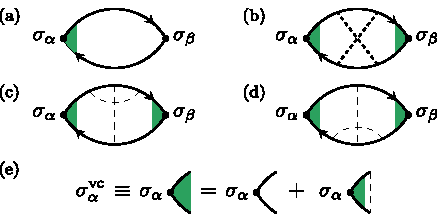
\includegraphics[]{articles/dirac_fm/fig2}
\caption{Diagrams considered in the calculation of $\hat{K}$: (a) non-crossing diagram, (b) $X$ diagram, (c-d) $\Psi$ diagrams. Green areas indicate the ladder summation (e) for the vertex correction in the non-crossing approximation \protect\cite{ivan}.}
\label{fig:diagrams}
\end{figure}

In our calculation the terms of the order of $\alpha \ln p_\textrm{cutoff}/\ep$ (where $p_\textrm{cutoff}$ is the ultraviolet momentum cut-off) is disregarded with respect to $1$. This approximation is legitimate since we assume that all model parameters $\epsilon$, $\Delta_\textrm{sd}$ and $\alpha$ are first renormalized such that $p_\textrm{cutoff} \approx \ep$.

It is, then, easy to see that the vertex-corrected spin operator is readily obtained from the geometric series of powers of $\pi\alpha \hat{M}$, 
\begin{align}
\sigma_\alpha^\text{vc} &= 
\sigma_\alpha+\pi\alpha \hat{M}_{\alpha\beta}\sigma_\beta+(\pi\alpha)^2 (\hat{M}^2)_{\alpha\beta}\sigma_\beta+\dots\nonumber\\
&=\left[1-\pi\alpha \hat{M}\right]^{-1}_{\alpha\beta}\sigma_\beta.
\end{align}
Thus, in the non-crossing approximation (illustrated in Fig.~\ref{fig:diagrams} (a)), one simply finds $\hat{K}= \hat{M}[1-\pi\alpha \hat{M}]^{-1}$. 
\cleardoublepage
\addtocontents{toc}{\protect\vspace{\beforebibskip}}%


\part{Ferromagnets}
%************************************************
\chapter{Introduction} % $\mathbb{ZNR}$
%************************************************
\section{Introduction}

A gapless character of the spin-wave spectrum in isotropic Heisenberg magnets in two dimensions results in the homogeneity of magnetic ordering being destroyed by thermal fluctuations at any finite temperatures. In contrast, in van der Waals magnets, characterized by intrinsic magnetocrystalline anisotropy that stems from spin-orbit coupling \cite{Lado2017}, an ordered magnetic state can be retained down to a monolayer limit. Two-dimensional (2D) van der Waals magnets are currently experiencing a revived attention \cite{Gong2017,Herrero2017,Burch2018,Tokmachev2018,Gong2019,Novoselov2019,Cortie2019} driven by the prospects of gateable magnetism \cite{Huang2018,Shengwei2018,Wang2018,Deng2018}, a continuing search for Kitaev materials \cite{Nagler2019,Gordon2019} and Majorana fermions \cite{Livanas2019}, topologically driven phenomena \cite{Mokrousov2019} as well as various applications \cite{Herrero2017,Burch2018,Novoselov2019}. The trade-off between quantum confinement, nontrivial topology and long-range magnetic correlations determines their unique magnetoelectronic properties, in particular a tunable tunneling conductance \cite{Wang2018a} and magnetoresistance \cite{Song2018,Klein2018,Kim2018} depending on the number of layers in the sample, as well as long-distance magnon transport \cite{Xing2019}. 

It is widely known that spin-orbit interaction provides an efficient way to couple electronic and magnetic degrees of freedom. It is, therefore, no wonder that the largest torque on magnetization, which is also referred to as the spin-orbit torque, emerges in magnetic systems with strong spin-orbit interaction \cite{miron_current-driven_2010,haney_current_2013} as has been long anticipated \cite{dyakonov_current-induced_1971}. 

The spin-orbit coupling may be enhanced by confinement potentials in effectively two-dimensional systems consisting of conducting and magnetic layers. The in-plane current may efficiently drive domain walls or switch magnetic orientation in such structures with the help of spin-orbit torque \cite{awschalom2009trend,manchon_theory_2008,garate_influence_2009,manchon2009theory}, which is present even for uniform magnetization, or with the help of spin-transfer torque, which requires the presence of magnetization gradient (due to e.\,g. domain wall) \cite{slonczewski_current-driven_1996,berger_emission_1996,ralph_spin_2008,stiles_anatomy_2002}. 

Topological insulators (TI) \cite{fu_topological_2007,moore_topological_2007,roy_topological_2009,hsieh_topological_2008} may be thought of as materials with an ultimate spin-orbit coupling. A closer look at the effective Hamiltonian for the conducting electrons at the TI/FM interface reveals that it indeed contains nothing but a spin-orbit interaction term that provides perfect spin-momentum locking. Thus, the magnetization dynamics in a thin ferromagnetic (FM) film in a proximity to TI surface is expected to be strongly affected by electric currents and/or electric fields \cite{qi_fractional_2008}. There seems to be a substantial experimental evidence that the efficiency of domain switching in TI/FM heterostructures is dramatically enhanced as compared to that in metals \cite{mellnik_spin-transfer_2014,wang_SOT_BiSe_2014,fan_magnetization_2014,Fan_SOT_TI_2016,Yasuda_SOT_BiSbTe_2017,Cha2018}. 


% \section{Dynamics of ferromagnets}
\vfill
\clearpage
\cleardoublepage
\addtocontents{toc}{\protect\vspace{\beforebibskip}}%

%************************************************
\chapter{Diffusive Spin-orbit torques in a two-dimensional Dirac ferromagnet}
%************************************************
In this chapter the spin-orbit torques on magnetization are investigated that occur when an insulating ferromagnetic (FM) layer is brought into close proximity to a topological insulator (TI). In addition to the well-known field-like spin-orbit torque, an anisotropic anti-damping-like spin-orbit torque is identified that originates in the diffusive motion of conduction electrons. This diffusive torque vanishes for a spatially homogeneous electric field or current, but may have a strong impact on spin-torque resonance at finite frequency provided that the external field is neither parallel nor perpendicular to the TI surface. The required electric field configuration to observe this effect can be created by a grated top gate.

\vfill
Parts of this chapter are published in Phys. Rev. \textbf{B} 99, 214444 (2019) 
\clearpage

% \maketitle
\section{introduction}
It is widely known that spin-orbit interaction provides an efficient way to couple electronic and magnetic degrees of freedom. It is, therefore, no wonder that the largest torque on magnetization, which is also referred to as the spin-orbit torque, emerges in magnetic systems with strong spin-orbit interaction \cite{miron_current-driven_2010,haney_current_2013} as has been long anticipated \cite{dyakonov_current-induced_1971}. 

The spin-orbit coupling may be enhanced by confinement potentials in effectively two-dimensional systems consisting of conducting and magnetic layers. The in-plane current may efficiently drive domain walls or switch magnetic orientation in such structures with the help of spin-orbit torque \cite{awschalom2009trend,manchon_theory_2008,garate_influence_2009,manchon2009theory}, which is present even for uniform magnetization, or with the help of spin-transfer torque, which requires the presence of magnetization gradient (due to e.\,g. domain wall) \cite{slonczewski_current-driven_1996,berger_emission_1996,ralph_spin_2008,stiles_anatomy_2002}. 

Topological insulators (TI) \cite{fu_topological_2007,moore_topological_2007,roy_topological_2009,hsieh_topological_2008} may be thought of as materials with an ultimate spin-orbit coupling. A closer look at the effective Hamiltonian for the conducting electrons at the TI/FM interface reveals that it indeed contains nothing but a spin-orbit interaction term that provides perfect spin-momentum locking. Thus, the magnetization dynamics in a thin ferromagnetic (FM) film in a proximity to TI surface is expected to be strongly affected by electric currents and/or electric fields \cite{qi_fractional_2008}. There seems to be a substantial experimental evidence that the efficiency of domain switching in TI/FM heterostructures is dramatically enhanced as compared to that in metals \cite{mellnik_spin-transfer_2014,wang_SOT_BiSe_2014,fan_magnetization_2014,Fan_SOT_TI_2016,Yasuda_SOT_BiSbTe_2017,Cha2018}. 

Nowadays the symmetry of spin-orbit torques is routinely inferred from the ferromagnetic resonance measurements in which an alternating microwave-frequency current (with frequencies $7-12$\,GHz) is applied within the sample plane \cite{mellnik_spin-transfer_2014,Ralph2011SOTFMresonance,Wang2015_SOTHflCoFEBIMgO,Ralph2016SOTWTE2,Ralph2018SOT}. 

In this work we identify a novel anti-damping-like torque originating in a diffusive motion of conduction electrons at the TI surface. Such a torque originates in a non-local diffusive response of the $z$-component of the conduction electron spin-density to the in-plane electric field. The non-locality of the response is determined by the so-called diffusion pole in analogy to the density-density response of a disordered system. It is, however, important that the diffusive response of the spin-density in the TI is always present in the perpendicular-to-the-plane component of the spin density, irrespective of the magnetization direction in the FM. In non-topological FM/metal systems such a diffusive response is present only in the spin density component that is directed along the local magnetization of the FM. Thus, the diffusive anti-damping spin-orbit torque, that we describe below, is specific for the TI/FM interfaces. Similarly, we identify a strong anisotropy of the Gilbert damping in the TI/FM system due to a combination of electron elastic scattering on non-magnetic impurities and a spin-momentum locking in the TI.  



The diffusive anti-damping spin-orbit torque, that we are going to study, can be related to the response of conduction electron spin-density to an electric field at a finite, but small, frequency and momentum. Such a field can be created e.\,g. by applying an \textit{ac} gate voltage to a grated top-gate as shown in Fig.~\ref{fig:setup}. The presence of the diffusive spin-orbit torque can be detected by rather unusual spin-orbit-torque resonances in the TI/FM structures that we also investigate in this work. 

%%%%%%%%%%%%
%%% figure 1
%%%%%%%%%%%%
\begin{figure}
\centering
\centerline{\hspace*{1cm}\includegraphics[width=0.8\linewidth]{{gfx/Chapter01/fig1.pdf}}}
\caption{Proposed experimental setup. Non-homogeneous in-plane electric field components are created by an $ac$ top-gate voltage $V_{\mathrm{top}}$ that  induce a strong diffusive spin-orbit torque (\ref{diffSOT}) of the damping-like symmetry. An effective magnetic field $\bb{H}$ is directed at the angle $\chi$ with respect to $\hat{\bb{z}}$.}
\label{fig:setup}
\end{figure}
%%%%%%%%%


Microscopic theory of current-induced magnetization dynamics in TI/FM heterostructures has been so far limited to some particular cases: (i) specific direction of magnetization and (ii) the limit of vanishing exchange interaction between FM angular momenta and the spins of conduction electrons.  In particular, an analytic estimate of spin-transfer and spin-orbit torques in TI/FM bilayer has been given in Ref.~\cite{sakai_spin_2014} for magnetization perpendicular to the TI surface. An attempt to generalize these results to arbitrary magnetization direction has been undertaken more recently in Ref.~\cite{ndiaye_dirac_2017}.  The non-local transport on a surface of the TI has been first discussed in Ref.~\cite{burkov_spin_2010-1}. The results of this work has been later applied to TI/FM systems \cite{taguchi_spin-charge_2015,shintani_spin_2016} in a perturbative approach with respect to a weak s--d-type exchange. The non-local behavior of non-equilibrium out-of-plane spin polarization in TI/FM systems, which gives rise to diffusive spin-orbit torques, have been, however, overlooked in all these publications. 

To describe magnetization dynamics at a TI/FM interface we employ an effective two-dimensional Dirac model for conduction electrons 
\be
\label{TImodel}
\mathcal{H}= v\,\lt[(\bb{p}-e\bb{A})\times \bb{\sigma}\rt]_z - \Delta_\textrm{sd}\, \bb{m}\cdot \bb{\sigma} +V(\bb{r}),
\e
where $\bb{A}$ stands for the vector potential, $e=-|e|$ is the electron charge, $z$ is the direction perpendicular to the TI surface, $v$ is the effective velocity of Dirac electrons, and $V(\bb{r})$ is a disorder potential that models the main relaxation mechanism of the conduction electrons momentum. The energy $\Delta_{\textrm{sd}}=J_\textrm{sd} S$ is characterizing the local exchange interaction $\mathcal{H}_\textrm{ex}=-J_\textrm{sd} \sum_n  \bb{S}_n \cdot c\h_n \bb{\sigma}c\0_n$ between localized classical magnetic moments $\bb{S}_n$ on FM lattice (with conserved absolute value $S=|\bb{S}_n|$ per unit cell area $\mathcal{A}$) and the electron spin-density  (represented by the vector operator $\bb{\sigma} = (\sigma_x,\sigma_y,\sigma_z)$ on the TI surface) \cite{sdmodel}. Here $\sigma_\alpha$ stand for Pauli matrices and $J_\textrm{sd}$ quantifies the s--d-type exchange interaction strength.  

Classical equation of motion for the unit magnetization vector $\bb{m}=\bb{S}/S$ is determined by the s-d like exchange interaction $\mathcal{H}_\textrm{ex}$ as
\be
\label{Eom}
\pa \bb{m}/\pa t = \gamma\, \bb{H} \times\bb{m}+\bb{T},\quad
\bb{T}=(J_\textrm{sd}\mathcal{A}/\hslash) \,\bb{m}\times\bb{s},
\e
where $\hslash=h/2\pi$ is the Planck constant and $\gamma$ is a gyromagnetic ratio for the FM spin. The effective field $\bb{H}$ represents the combined contribution of external magnetic field and the field produced by neighboring magnetic moments in the FM (e.\,g. due to direct exchange), while the term $\bb{T}$ represents the effect of the conduction electron spin density $\bb{s}(\bb{r},t)= \la c\h_n \bb{\sigma} c\0_n\ra$  on the TI surface. 

To quantify the leading contributions to $\bb{T}$ we microscopically compute: i) a linear response of $\bb{s}$ to the in-plane electric field $\bb{E}(\bb{r},t)= \bb{E}_{\bb{q},\omega}\exp\lt(-i\omega t+i\bb{q}\cdot\bb{r}\rt)$; and ii) a linear response of $\bb{s}$  to the time derivative $\pa \bb{m}/\pa t$. The former response defines the spin-orbit torque, while the latter one does the Gilbert damping. 
 
Before we proceed with the analysis we shall note that the velocity operator $\bb{v} = v\,(\bb{\sigma}\times \hat{\bb{z}})$ in the model of Eq.~(\ref{TImodel})  is directly related to the spin operator $\bb{\sigma}$. As the result, the response of the in-plane spin density $\bb{s}_\parallel=(s_{x}, s_{y})$ to electric field $\bb{E}=-\pa\bb{A}/\pa t$ is defined by the conductivity tensor \cite{ndiaye_dirac_2017,Ghosh18}. This also means that the non-equilibrium contribution to $\bb{s}_\parallel$ from the electric current density $\bb{J}$ is given by $\bb{s}_\parallel= (\hat{\bb{z}}\times\bb{J} )/ev$ for any frequency and momentum irrespective of type of scattering for conduction electrons and even beyond the linear response. 

Thus, the response of $\bb{s}_\parallel$ defines an exceptionally universal field-like spin-orbit torque
\be
\label{TFL}
\bb{T}^\textrm{SOT}_\textrm{FL}= (J_\textrm{sd}\mathcal{A}/\hslash e v)\, \bb{m}\times(\hat{\bb{z}}\times\bb{J}),
\e 
that acts in the same way as in-plane external magnetic field applied perpendicular to the charge current. 

Apart from the universal response of $\bb{s}_\parallel$ there might also exists a non-equilibrium spin polarization $s_z$ perpendicular to the TI surface. This component plays no role in Eq.~(\ref{Eom}) for $\bb{m}= \pm \hat{\bb{z}}$ due to the vector product involved. Also, the $s_z$ component is vanishing by symmetry for $\bb{m}=\bb{m}_\parallel$, where we decompose $\bb{m} =\bb{m}_\parallel+\bb{m}_\perp$ to in-plane and perpendicular-to-the plane components.

We find, however, that for a general direction of $\bb{m}$, the spin density $s_z$ may be strongly affected by the in-plane electric field at a small but finite frequency and a small but finite wave vector. In the leading approximation the result can be cast in the following form 
\be
\label{diffSOT}
\bb{T}^\textrm{SOT}_\textrm{diff} = \eta\, \bb{m}\times\bb{m}_\perp\, \frac{i D\, \bb{q}\cdot \bb{E}}{i\omega -Dq^2},\quad
\eta=\frac{eJ_\textrm{sd}^2\mathcal{A}S}{2\pi \hslash^3v^2},
\e
where $D$ is a diffusion coefficient for conduction electrons at the TI surface and $\bb{E}= \bb{E}_{\bb{q},\omega}\exp\lt(-i\omega t+i\bb{q}\cdot\bb{r}\rt)$. Note that the diffusive torque is non-linear with respect to $\bb{m}$ and, from the point of view of the time reversal symmetry, is analogous to anti-damping torque. The denominator $i\omega -Dq^2$ in Eq.~(\ref{diffSOT}) reflects diffusive (Brownian) motion of conduction electrons that defines the time-delayed diffusive torque on magnetization $\bb{T}^\textrm{SOT}_\textrm{diff}$.  

It is interesting to note that the torque of Eq.~(\ref{diffSOT}) has an anti-damping symmetry (when expressed through electric current rather than electric field). Moreover, the torque formally diverges as $1/q$ in the $dc$ limit $\omega=0$. This singularity is well-known in the theory of disordered systems \cite{maleev1975corrections,maleev1976corrections,altshuler1985electron} and originates in the diffusive (Brownian) motion of conduction electrons in a disorder potential.  The $dc$ limit singularity in Eq.~(\ref{diffSOT}) is, in fact, regularized by the dephasing length of conduction electrons on the surface of the TI. The length is strongly temperature and material dependent and, at low temperatures, can reach hundreds of microns. Thus, the result of Eq.~(\ref{diffSOT}) also predicts large anti-damping spin-orbit torque in the dc-limit that originates in a mechanism which is specific for the TI interface. 

\section{model}
In order to derive the result of Eq.~(\ref{diffSOT}) and the expressions for Gilbert damping we shall adopt a particular relaxation model for both spin and orbital angular momenta of conduction electrons. For the model of Eq.~(\ref{TImodel}) those are provided by scattering on disorder potential. We choose the latter 
to be the white-noise Gaussian disorder potential that is fully characterized by a single dimensionless parameter $\alpha\ll 1$,
\be
\label{disorder}
\la V(\bb{r})\ra =0,\quad \la V(\bb{r}) V(\bb{r}') \ra = 2\pi \alpha\, (\hslash v)^2\,\delta(\bb{r}-\bb{r}'),
\e
where angular brackets stay for the averaging over the ensemble of disordered systems. 

Since both the vector potential $\bb{A}$ and the magnetization $\bb{m}$ couple to spin operators in Eq.~(\ref{TImodel}), the linear response of $\bb{s}$ to $\bb{E}=-\pa\bb{A}/{\pa t}$ and $\pa \bb{m}/\pa t$ is defined in the frequency-momentum domain as 
\be
\label{spol}
\bb{s} =(v^2 h)^{-1} \hat{K}(\bb{q},\omega) \lt[e v\,(\bb{E}\times \hat{\bb{z}}) - i \omega\Delta_\textrm{sd}\,\bb{m} \rt].
\e
Here, the dimensionless 9-component tensor $\hat{K}(\bb{q},\omega)$ is given by the Kubo formula 
\be
\label{Kubo}
\hat{K}_{\alpha\beta}(\bb{q},\omega)= {v^2}\!\!\int\!\! \frac{d^2\bb{p}}{(2\pi)^2}
\tr \lt\la \sigma_\alpha G^\textrm{R}_{\bb{p}+\hslash \bb{q},{\ep+\hslash\omega}}\sigma_\beta G^\textrm{A}_{\bb{p},\ep}\rt \ra,
\e
where the notation $G^{\textrm{R(A)}}_{\bb{p},\ep}$ stands for the retarded (advanced) Green's function for the Hamiltonian of Eq.~(\ref{TImodel}), the angular brackets denote the averaging over disorder realizations, while the energy $\ep$ refers to the Fermi energy (zero temperature limit is assumed). 

The tensor $\hat{K}$ can be represented by the matrix 
\be
\label{Kten}
\hat{K}=  
\bpm \sigma_{xx} & \sigma_{xy} & Q_y \\ \sigma_{yx} & \sigma_{yy} & -Q_x \\ Q_y & -Q_x & \zeta \epm,
\e
of which $\sigma_{\alpha\beta}$ are the components of the two dimensional conductivity tensor at the TI surface (all conductivities are expressed in the units of $e^2/h$),  the vector $\bb{Q}$ defines the diffusive spin-orbit torque of Eq.~(\ref{diffSOT}) (its contribution to Gilbert damping is negligible), while $\zeta$ determines the response of $s_z$ to $\pa m_z/\pa t$. The components of $\hat{K}$ correspond to different responses at different limits. When discussing the response to an electric field $\bb{E}_{\bb{q}\omega}$ we are primarily interested in the limit $\omega\ll Dq^2$, whereas the response to time-derivative of magnetization $\bb{m}$ is defined by the limit $q\to 0$. 


In the linear response theory of Eq.~(\ref{spol}) one needs to compute the tensor in Eq.~(\ref{Kubo}) for a constant direction $\bb{m}$ and for $\bb{A}=0$. In usual systems (conducting ferromagnets) the response of $\bb{s}$ in the direction of $\bb{m}$ is always diffusive. This response, however, plays no role in the torque since $\bb{T}\propto \bb{m}\times \bb{s}$. The situation at the TI surface is, however, special. Here, the in-plane components of magnetization $m_x, m_y$ play no role in Eq.~(\ref{TImodel}), since those are simply equivalent to a constant in-plane vector potential for conduction electrons and, therefore, can be excluded by a gauge transform (shift of the Dirac cone). Consequently, all observable quantities in the model (including all components of the tensor $\hat{K}$) may only depend on the field $\Delta_z=\Delta_\textrm{sd} m_z$. As the result, the diffusive response occurs exclusively in $s_z$ component of spin polarization and can easily enter the expression for the torque.

The conductivity tensor in the model of Eqs.~(\ref{TImodel},\ref{disorder}) has been analyzed in detail in Ref.~\cite{ivan} in the limit $\omega=\bb{q}=0$ (and for $\alpha\ll 1$) with the result $\sigma_{xx}=\sigma_{yy}=\sigma_0$ and $\sigma_{xy}=-\sigma_{yx}=\sigma_\textrm{H}$, where  
\be
\label{cond}
\sigma_0= \frac{\ep^2-\Delta_z^2}{\pi\alpha\,(\ep^2+3\Delta_z^2)},\qquad \sigma_\textrm{H}= \frac{8 \ep \Delta_z^3}{(\ep^2+3\Delta_z^2)^2}.
\e
Since the anomalous Hall conductivity $\sigma_\textrm{H} \propto \alpha\, \sigma_0$ is sub-leading with respect to $\sigma_0$, it has to be computed beyond the Born approximation (see Refs.~\cite{ivan,ivanPRL,ivanPRB}). 

Here we generalize the analysis to calculate the tensor $\hat{K}$ for finite $\omega$ and $\bb{q}$ assuming $\alpha\ll 1$, $\omega\tau_\textrm{tr}\ll 1$, and $\omega \propto Dq^2$, where $D=\hslash v^2  \sigma_0/\ep$ is the diffusion coefficient and $\tau_\textrm{tr}=\hslash\ep\sigma_0/(\ep^2+\Delta_z^2)$ is the transport scattering time for the problem. In real samples $\tau_\textrm{tr}=0.01 - 1$\,ps \cite{kong_rapid_2011,kamboj_probing_2017,huang_enhancement_2017,xiang_transport_2014}.

The main building block of our analysis is the averaged Green's function in the first Born approximation
\be
\label{green}
G^{\mathrm{R}}_{\bb{p},\ep} = \frac{\ep^\textrm{R} + v(\bb{p}\times \bb{\sigma})_z-\Delta^{\textrm{R}}_z\sigma_z}
{(\ep^{\textrm{R}})^2-v^2p^2 -(\Delta^{\textrm{R}}_z)^2},
\e
where the complex parameters $\ep^\textrm{R}=\ep(1+i\pi \alpha/2)$ and  $\Delta^\textrm{R}_z= \Delta_z(1-i\pi \alpha/2)$ are found from the corresponding self-energy 
\be
\label{Sigma}
\Sigma^{\mathrm{R}}(\ep)  = 2\pi \alpha\,v^2\!\! \int\!\frac{d^2\bb{p}}{(2\pi)^2}G^\mathrm{R}_{\bb{p},\ep}, 
\e
that gives rise to  $\im \Sigma^{\mathrm{R}}= - \pi \alpha (\ep -\Delta_z \sigma_z)/2$  (strictly speaking, the RG analysis \cite{ivan} has to be applied). In the Green's function of Eq.~(\ref{green}) we shift the momentum $\bb{p}$ such that there is no direct dependence on the in-plane magnetization components $m_x$ and $m_y$. 

The next step in disorder-averaging requires the computation of vertex corrections. This means we need to replace the spin operator $\sigma_\alpha$ with a vertex corrected spin operator $\sigma_\alpha^\text{vc}$ in the ladder approximation as depicted in Fig.~\ref{fig:diagrams}(e). The crossed diagrams in Fig.~\ref{fig:diagrams}(b-d) give a contribution to the components of $\hat{K}$ of the order $\mathcal{O}(\alpha^0)$. The
only components that are modified to this order are those
corresponding to the Hall conductivity (i.e. $\sigma_{xy}$ and $\sigma_{yx}$). Details of this calculation can be found Ref.~\cite{ivan}.
%

The dressing of $\sigma_\alpha$ with a single disorder line is denoted by $\sigma_\alpha^{1\times\text{dr}}$ and is conveniently represented in the matrix form by introducing a matrix $\hat{M}$ with $16$ components $M_{\alpha\beta}$ for $\alpha,\beta=0,x,y,z$ (with $\sigma_0=1$)
    \begin{align}
       \sigma_\alpha^{1\times\text{dr}}  = 2\pi \alpha\, v^2 \int\!\frac{d^2\bb{p}}{(2\pi)^2} G^\text{A}_{\ep+\omega,\bb{p}+\bb{q}}\sigma_\alpha G^\text{R}_{\bb{p}} = \pi\alpha M_{\alpha\beta}\sigma_\beta,
        \label{chap1:eq:myseries}
    \end{align}
where the summation of the repeating index $\beta=0,x,y,z$ is assumed. Full expressions of the components of $\hat{M}$ up to second order in $\omega$ and $q$ are given by Eq.~(\ref{chap1:eq:M}a-f). 
%%%
% Fig. 2
%%%
\begin{figure}[t]
\centering
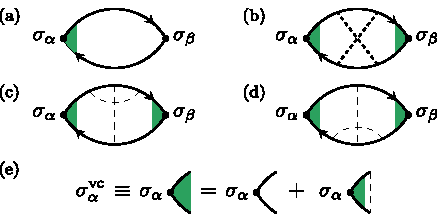
\includegraphics[]{articles/dirac_fm/fig2}
\caption{Diagrams considered in the calculation of $\hat{K}$: (a) non-crossing diagram, (b) $X$ diagram, (c-d) $\Psi$ diagrams. Green areas indicate the ladder summation (e) for the vertex correction in the non-crossing approximation \protect\cite{ivan}.}
\label{fig:diagrams}
\end{figure}

In our calculation the terms of the order of $\alpha \ln p_\textrm{cutoff}/\ep$ (where $p_\textrm{cutoff}$ is the ultraviolet momentum cut-off) is disregarded with respect to $1$. This approximation is legitimate since we assume that all model parameters $\epsilon$, $\Delta_\textrm{sd}$ and $\alpha$ are first renormalized such that $p_\textrm{cutoff} \approx \ep$.

It is, then, easy to see that the vertex-corrected spin operator is readily obtained from the geometric series of powers of $\pi\alpha \hat{M}$, 
\begin{align}
\sigma_\alpha^\text{vc} &= 
\sigma_\alpha+\pi\alpha \hat{M}_{\alpha\beta}\sigma_\beta+(\pi\alpha)^2 (\hat{M}^2)_{\alpha\beta}\sigma_\beta+\dots\nonumber\\
&=\left[1-\pi\alpha \hat{M}\right]^{-1}_{\alpha\beta}\sigma_\beta.
\end{align}
Thus, in the non-crossing approximation (illustrated in Fig.~\ref{fig:diagrams} (a)), one simply finds $\hat{K}= \hat{M}[1-\pi\alpha \hat{M}]^{-1}$. 

Dressed spin-spin correlators are defined by the components $ \hat{K}_{\alpha\beta}$ with $\alpha,\beta=x,y,z$.
The vector $\bb{q}$ selects a particular direction in space, that makes the conductivity tensor anisotropic. By choosing $x$ direction along the $\bb{q}$ vector, we find the conductivity components $\sigma_{xx} = \sigma_0$, $\sigma_{xy} = -\sigma_{yx}=\sigma_\textrm{H}$, and $\sigma_{yy}= i\omega \,\sigma_0/(i\omega-Dq^2)$, where we have kept only the leading terms in the limits $\alpha\ll 1$, $\omega\tau_\textrm{tr}\ll 1$ (more general expressions are given by Eqs.~(\ref{chap1:eq:sconductivity}a-d)). We can see that $\sigma_{yy}$ component also acquires a diffusion pole.  One needs to go beyond the non-crossing approximation in the computation of anomalous Hall conductivity  \cite{ivan,ivanPRL,ivanPRB}. 

Clearly, the components $\sigma_{\alpha\beta}$ define the field-like contribution $\bb{T}^\textrm{SOT}_\textrm{FL}$ that has been already discussed above. It is interesting to note that the conductivity is isotropic $\sigma_{xx}=\sigma_{yy}=\sigma_0$ only if the limit $q= 0$ is taken before the limit $\omega=0$. If the limit $\omega=0$ is taken first, the conductivity remains anisotropic with respect to the direction of $\bb{q}$ even for $q=0$.

The vector $\bb{Q}=(Q_x,Q_y)$ quantifies both the response of $s_z$ to electric field or to $\pa \bb{m}_\parallel/\pa t$ as well as the response of $\bb{s}_\parallel$ to  $\pa m_z/\pa t$. From Eq.~(\ref{Kubo}) we find,
\be
\label{Qvec}
\bb{Q}(\omega,\bb{q})=\frac{\Delta_z}{\hslash v}\, \frac{i D \bb{q}}{i\omega-Dq^2}\lt(1+\mathcal{O}(\omega\tau_\textrm{tr})\rt),
\e
where we again assumed $\omega\tau_\textrm{tr} \ll 1$. The result of Eq.~(\ref{Qvec}), then, corresponds to an additional diffusive spin-orbit torque of the form Eq.~(\ref{diffSOT}).

Finally, the response of $s_z$ to $\pa m_z/\pa t$ is defined by 
\be
\label{szz}
\zeta = \frac{\Delta_z^2}{i\hslash\ep\omega}\lt(1+\mathcal{O}(\omega^2\tau^2_\textrm{tr})\rt),
\e
where the limit $q=0$ is taken. Thus, we find from Eq.~(\ref{spol}) that there exists no response of $s_z$ to $\pa m_z/\pa t$. Instead, the quantity $\zeta$ defines the additional spin polarization in $z$-direction $\delta s_z = - \Delta_\textrm{sd}^3m_z^3/(2\pi \hslash^2 v^2\ep)$ that we ignore below. Eqs.~(\ref{Qvec},\ref{szz}) including subleading terms in $\omega\tau_\mathrm{tr}$ are presented in Eq.~(\ref{Qresult}).

We also note, that $\bb{Q}(q=0)=0$, hence there is no term in $s_z$ that is proportional to $\pa\bb{m}/\pa t$. This reflects highly anisotropic nature of the Gilbert damping in the model of Eq.~(\ref{TImodel}).

The remaining parts of the Gilbert damping can be cast in the following form 
\be
\bb{T}^\textrm{GD}=\frac{J^2_\textrm{sd} \mathcal{A} S}{\pi\hslash^2 v^2}\,\bb{m}\times
\Big(\sigma_0\,\frac{\pa \bb{m}_\parallel}{\pa t} + \frac{\sigma_\textrm{H}}{m_z}\, \frac{\pa \bb{m}_\parallel}{\pa t}\times\bb{m}_\perp \Big),
\label{GD}
\e
where the coefficients, $\sigma_0$ and $\sigma_\textrm{H}/m_z$ from Eq.~(\ref{cond}) depend on $m_z^2$, which is yet another source of the Gilbert damping anisotropy.  We note, that even though Eq.~(\ref{GD}) does not contain a term proportional to $\partial m_z/\partial t$, the existing in-plane Gilbert damping is sufficient to relax the magnetization along $\hat{\bb{z}}$ direction. 

Despite strongly anisotropic nature of the diffusive torque (the torque is vanishing for purely in-plane or purely perpendicular to the plane magnetization), its strength for a generic direction of magnetization may be quite large. For example, for $\bb{m}$ directed approximately at 45 degrees to the TI surface the ratio of amplitudes of diffusive and field like torques is readily estimated as  
\be
\label{estimate}
\frac{T^\textrm{SOT}_\textrm{diff}}{T^\textrm{SOT}_\textrm{FL}} = \frac{\Delta_\textrm{sd}}{\hslash q v}\,\frac{1}{\sigma_0},
\e
where we used the condition $\omega \ll Dq^2$.  Let us assume that a top-gate in Fig.~\ref{fig:setup} induces an ac in-plane electric field with the characteristic period $2\pi q^{-1}\approx 1$\,$\mu$m and a typical FM resonance frequency, $\omega\approx 7$-$12$\,GHz. Then, for realistic materials one can estimate $Dq^2\approx 100$\,GHz, hence $\omega \ll Dq^2$ indeed. For a typical velocity $v=10^6$\,m$/$s one finds  $\hslash q v\approx 4$\,meV. Thus, the ratio $\Delta_\textrm{sd}/\hslash q v$ in Eq.~(\ref{estimate}) may reach three orders of magnitude, while the value of $\sigma_0$ is typically $10$. This estimate suggests that, for a generic direction of $\bb{m}$, the magnitude of diffusive  torque can become three orders of magnitude larger than that of the field-like spin-orbit torque. 

The diffusive torque at the TI surface can be most directly probed by the corresponding spin-torque resonance. In this case, one can disregard the effect of the field like torque, so that Eq.~(\ref{Eom}) is simplified to
\be
\label{equation}
\frac{\pa \bb{m}}{\pa t}=\gamma\,\bb{H}\times \bb{m}+f(\bb{r},t)\,\bb{m}\times\bb{m}_\perp+\alpha_\textrm{G}\,\bb{m}\times\frac{\pa \bb{m}_\parallel}{\pa t},
\e
where $\alpha_\textrm{G}= J_\textrm{sd}^2 \mathcal{A}S \sigma_0/\pi(\hslash v)^2$ is the Gilbert damping amplitude (which is a constant for $\ep \gg \Delta_\textrm{sd}$), while the terms containing $\sigma_\textrm{H}$ are omitted.  The function
\be
f(\bb{r},t)=\eta\int\! d^2\bb{r}'\!\!\int_{-\infty}^t\!\!\!\! dt'\, \frac{e^{-(\bb{r}-\bb{r}')^2/4D(t-t')}}{4\pi(t-t')}\bb{\nabla}\cdot\bb{E}(\bb{r}',t'),\n
\e
defines the strength of the diffusive spin-orbit torque (\ref{diffSOT}) in real space and time.

Resonant magnetization dynamics defined by Eq.~(\ref{equation}) is illustrated in Fig.~\ref{fig:dynamics} for $\bb{H}$ directed at the angle $\chi =\pi/4$ with respect to $\hat{\bb{z}}$ and for frequencies that are close to the resonant frequency $\omega_0=\gamma H$. The time evolution of magnetization projection $m_\textrm{H}= \bb{m}\cdot \bb{H}/H$ is induced by the diffusive torque with $f(t)= f_0\,\cos\omega t$ (magnetization at different $\bb{r}$ is simply different by a phase). 

%%%%%%%%%%%%
%%% figure 3
%%%%%%%%%%%%
\begin{figure}
\centering
\centerline{\hspace*{1cm}\includegraphics[width=1.0\linewidth]{{articles/dirac_fm/fig3}}}
\caption{The projection $m_\textrm{H}(t)$ as simulated from Eq.~(\ref{equation}) for $f_0=0.1\, \omega_0$.  Top panel illustrates the behavior at different frequencies for $\alpha_\textrm{G}=0.005$. Lower panel illustrates the resonant behavior at different values of $\alpha_\textrm{G}$. Dashed horizontal line corresponds to $m_\textrm{H}=1/\sqrt{2}$. Dots indicate the asymptotic solution for $\alpha_\textrm{G}=0$ as given by Eq.~(\ref{asymptot}).}
\label{fig:dynamics}
\end{figure}
%%%%%%%%%

Resonant dynamics at $\omega=\omega_0$ in Eq.~(\ref{equation}) consists of precession of $\bb{m}$ around the vector $\bb{H}$ such that the azimut (precession) angle is changing linearly with time $\phi(t)=\omega_0 t-\pi/2$  (for $f_0\ll \omega_0$ and $\alpha_\textrm{G}\ll1$). In addition, the projection $m_\textrm{H}$ oscillates between $1$ and $0$ on much larger time scales. Such oscillations are damped by a finite $\alpha_\textrm{G}$ to the limiting value $m_\textrm{H}=1/\sqrt{2}$. 

In the limit of vanishing Gilbert damping, $\alpha_\textrm{G}=0$, one simply finds the result 
\be
\label{asymptot}
m_\textrm{H}(t)=\lt[\cosh\lt(\tfrac{1}{4}f_0 t \sin (2\chi) \rt)\rt]^{-1},
\e
which clearly illustrates the absence of the effect for both perpendicular-to-the-plane ($\chi=0$) and in-plane ($\chi=\pi/2$) magnetization. The qualitative behavior at the resonance ($\omega=\omega_0$) is illustrated at the lower panel of Fig.~\ref{fig:dynamics} for different values of $\alpha_\textrm{G}$.

\section{Conclusions}
In conclusion, we consider magnetization dynamics in a model TI/FM system at a finite frequency $\omega$ and $\bb{q}$ vector. We identify novel diffusive anti-damping spin-orbit torque that is specific to TI/FM system.  Such a torque is absent in usual (non-topological) FM/metal systems, where the diffusive response of conduction electron spin density is always aligned with the magnetization direction of the FM. In contrast, the electrons at the TI surface gives rise to singular diffusive response of the conduction electron spin-density in the direction perpendicular to the TI surface, irrespective of the FM magnetization direction. Such a response leads to strong non-adiabatic anti-damping spin-orbit torque that has a diffusive nature. This response is specific for a system with an ultimate spin-momentum locking and gives rise to abnormal anti-damping diffusive torque that can be detected by performing spin-torque resonance measurements. We also show that, in realistic conditions, the anti-damping like diffusive torque may become orders of magnitude larger than the usual field like spin-orbit torque. We investigate the peculiar magnetizations dynamics induced by the diffusive torque at the frequency of the ferromagnet resonance. Our theory also predicts ultimate anisotropy of the Gilbert damping in the TI/FM system. In contrast, to the phenomenological approaches \cite{vanderBijl2012,Hals2013} our microscopic theory is formulated in terms of very few effective parameters. Our results are complementary to previous phenomenological studies of Dirac ferromagnets \cite{tserkovnyak_theory_2009,mahfouzi_spin-orbit_2012,katsnelson15,fischer_spin-torque_2016,yokoyama_theoretical_2010,yokoyama_current-induced_2011,siu_spin_2016,mahfouzi_antidamping_2016,soleimani_spin-orbit_2017,kurebayashi_microscopic_2017,chen_current-induced_2017,rodriguez-vega_giant_2016,qi_topological_2008,garate_inverse_2010,yokoyama_theoretical_2010,yokoyama_current-induced_2011,nomura_electric_2010,tserkovnyak_thin-film_2012-1,linder_improved_2014,tserkovnyak_spin_2015,ueda_topological_2012,liu_reading_2013,chang_nonequilibrium_2015,fischer_spin-torque_2016,mahfouzi_antidamping_2016,fujimoto_transport_2014,okuma_unconventional_2016}.

 % Diffusive spin-orbit torques in a Dirac ferromagnet
\cleardoublepage
\addtocontents{toc}{\protect\vspace{\beforebibskip}}%


\part{Antiferromagnets}
%************************************************
\chapter{Antiferromagnets} % $\mathbb{ZNR}$
%************************************************
\section{Introduction}
An increasing demand for ever higher performance computation and ever faster big data analytics has sparked recently the interest to antiferromagnetic spintronics \cite{macdonald_antiferromagnetic_2011, gomonay_spintronics_2014, wadley_electrical_2016, jungwirth_antiferromagnetic_2016, baltz_antiferromagnetic_2018, jungwirth_multiple_2018, jungfleisch_perspectives_2018}, i.\,e. to the usage of much more subtle antiferromagnetic order parameter to store and process information. This idea is driven primarily by the expectation that antiferromagnetic materials may naturally allow for up to THz operation frequencies \cite{gomonay_high_2016, olejnik_terahertz_2018, jungwirth_multiple_2018} in sharp contrast to ferromagnets whose current-induced magnetization dynamics is fundamentally limited to GHz frequency range. 
  
The best efficiency in electric switching of magnetic domains is achieved in systems involving materials with at least partial spin-momentum locking \cite{fina_electric_2017} due to sufficiently strong spin-orbit interaction. The latter is responsible for the so-called spin-orbit torques on magnetization that are caused by sizable non-equilibrium spin polarization induced by an electron flow \cite{brataas_current-induced_2012, Hals2013, zelezny_relativistic_2014, freimuth_spin-orbit_2014, ghosh_spin-orbit_2017, smejkal_electric_2017, zelezny_spin_2018, zhou_strong_2018, manchon_current-induced_2019, moriyama_spin-orbit-torque_2018, li_manipulation_2019, chen_electric_2019, zhou_large_2019, zhou_fieldlike_2019, bodnar_writing_2018}.  

Recently, spin-orbit-torque-driven electric switching of the N\'eel vector orientation has been predicted \cite{zelezny_relativistic_2014} and discovered in non-centrosymmetric crystals such as CuMnAs \cite{wadley_electrical_2016, fina_electric_2017, zelezny_spin_2018, saidl_optical_2017} and Mn$_2$Au \cite{barthem_revealing_2013, jourdan_epitaxial_2015, bhattacharjee_neel_2018}. Even though many antiferromagnetic compounds are electric insulators \cite{pandey_doping_2017}, which limits the range of their potential applications, e.\,g., for spin injection \cite{tshitoyan_electrical_2015}, the materials like CuMnAs and Mn$_2$Au possess  semi-metal and metal properties, inheriting strong spin-orbit coupling and sufficiently high conductivity. These materials also give rise to collective mode excitations in THz range \cite{bhattacharjee_neel_2018}. 

Spin-orbit torque in antiferromagnets have been investigated theoretically using Kubo-Streda formula in the case of two-dimensional (2D) Rashba gas, as well as in tight-binding models of Mn$_2$Au \cite{zelezny_relativistic_2014, zelezny_spin-orbit_2017}. These pioneering works describe the spin-orbit torques based on their influence on the current-driven dynamics as predicted by Landau-Lifshitz-Gilbert equation. In particular, they proposed that only a staggered field-like torque and an non-staggered anti-damping torque can trigger current-driven antiferromagnetic THz switching and excitation in antiferromagnets (see e.\,g., \cite{fjaerbu_electrically_2017, cheng_terahertz_2016, khymyn_antiferromagnetic_2017}). This analysis served as a basis to further investigation of spin-orbit torques in heterostructures \cite{manchon_spin_2017, ghosh_spin-orbit_2017, ghosh_nonequilibrium_2019}. Furthermore, a symmetry group analysis has been developed to predict the form of these two components based on the magnetic point groups of the antiferromagnets \cite{zelezny_spin-orbit_2017, watanabe_symmetry_2018}. 
 
In the context of current-driven antiferromagnetic domain wall \cite{hals_phenomenology_2011} and skyrmion motion \cite{barker_static_2016, zhang_antiferromagnetic_2016}, the N\'eel vector dynamics has been modeled within the phenomenological treatment of the Landau-Lifshitz-Gilbert equation pioneered by Slonczewski \cite{slonczewski_current-driven_1996}. In this phenomenological approach the torques on magnetization derived above have been simply postulated \cite{gomonay_high_2016, shiino_antiferromagnetic_2016, akosa_theory_2018, tomasello_performance_2017}. 


Moreover, it has recently been suggested that current technology may have a lot to gain from antiferromagnet (AFM) materials. Indeed, manipulating AFM domains does not induce stray fields and has no fundamental speed limitations up to THz frequencies \cite{jungwirth_antiferromagnetic_2016}. 

Despite their ubiquitousness, AFM materials have, however, avoided much attention from technology due to an apparent lack of control over the AFM order parameter -- the N\'eel vector. Switching the N\'eel vector orientation by short electric pulses has been put forward only recently as the basis for AFM spintronics \cite{macdonald_antiferromagnetic_2011,gomonay_spintronics_2014,zelezny_relativistic_2014}. 
The proposed phenomenon has been soon observed in non-centrosymmetric crystals such as CuMnAs \cite{wadley_electrical_2016, fina_electric_2017, zelezny_spin_2018, saidl_optical_2017} and Mn$_2$Au \cite{barthem_revealing_2013, jourdan_epitaxial_2015, bhattacharjee_neel_2018}. It should be noted that in most cases AFMs are characterized by insulating type behavior \cite{pandey_doping_2017}, limiting the range of their potential applications, e.g., for spin injection \cite{tshitoyan_electrical_2015}. Interestingly, antiferromagnetic Mn$_2$Au possesses a typical metal properties, inheriting strong spin-orbit coupling and high conductivity, and is characterized by collective modes excitations in THz range \cite{bhattacharjee_neel_2018}.

Despite a lack of clarity concerning the microscopic mechanisms of the N\'eel vector switching, these experiments have been widely regarded as a breakthrough in the emerging field of THz spintronics \cite{bhattacharjee_neel_2018, gomonay_high_2016, olejnik_terahertz_2018, jungwirth_multiple_2018, wadley_electrical_2016, jungwirth_antiferromagnetic_2016, baltz_antiferromagnetic_2018, jungfleisch_perspectives_2018}. It has been suggested that current-induced N\'eel vector dynamics in an AFM is driven primarily by the so-called N\'eel spin-orbit torques \cite{brataas_current-induced_2012, Hals2013, zelezny_relativistic_2014, freimuth_spin-orbit_2014, ghosh_spin-orbit_2017, smejkal_electric_2017, zelezny_spin_2018, zhou_strong_2018, manchon_current-induced_2019, moriyama_spin-orbit-torque_2018, li_manipulation_2019, chen_electric_2019, zhou_fieldlike_2019, zhou_large_2019, bodnar_writing_2018}. The N\'eel spin-orbit torque originates in a non-equilibrium staggered polarization of conduction electrons on AFM sublattices \cite{zelezny_relativistic_2014, smejkal_electric_2017, zelezny_spin_2018, manchon_current-induced_2019}. Characteristic magnitude of the non-equilibrium staggered polarization and its relevance for the experiments with CuMnAs and Mn$_2$Au remain, however, debated. 

\section{Antiferromagnetic resonance}
One of the characteristics of an antiferromagnets is that its antiferromagnetic resonance frequency (i.e. when subjected to an oscillating external magnetic field) is proportional to $\sqrt{K}$, as given by the formula:
\begin{equation}
    \omega = \gamma_0 H_\text{ext} \pm \sqrt{K(J+K)}
\end{equation}
as first derived by Kittel \cite{kittel}. The original derivation made use of quadrupolar contributions to $H_\text{M}$, but for two dimensional systems, a Hamiltonian such as in Eq.~(\ref{intro:eq:Hm}) is sufficient as we will demonstrate. In this section we do not consider $\Delta_\text{sd}$. In order to find the resonant frequencies in the system that is subjected to an oscillating field in the $z$ direction: $\bb{H}_\text{ext} = H_0 \cos \omega t\,\hat{\bb{z}}$, we first linearize the equations of motion by expanding $\bb{n}$ close to $\hat{\bb{z}}$ and assume $\bb{m}$ to be small. To be more explicit
\begin{equation}
	\bb{n} \rightarrow \bb{z} + \delta \bb{n}_\parallel,\quad \bb{m} \rightarrow \delta \bb{m}_\parallel.
\end{equation}
Note that to first order the staggered and non-staggered magnetizations are still orthogonal to each-other: $\bb{n}\cdot\bb{m}=1+\mathcal{O}(\delta n^2+\delta m^2)$. Components such as $\delta n_x \delta m_y$ can be then disregarded and we assume $\bb{n}$ and $\bb{m}$ to be proportional to $\exp i \omega t$. A nice basis to work in is $\{{n}_+,{m}_+,{n}_-,{m}_- \}$, (where ${n}_\pm = \delta n_x\pm i \delta n_y$ and ${m}_\pm = \delta m_x\pm i \delta m_y$) so that one finds the following matrix equation:
\begin{equation}
    \begin{pmatrix}
    \omega_0 & -(J+K) & 0 & 0 \\
    -K & \omega_0 & 0 & 0 \\
    0 & 0 & -\omega_0 & J+K \\
    0 & 0 & K & -\omega_0
    \end{pmatrix}
    \begin{pmatrix}
    \delta l_{+}\\
    \delta m_{+}\\
    \delta l_{+}\\
    \delta m_{-}
    \end{pmatrix}
    =\omega 
    \begin{pmatrix}
    \delta l_{+}\\
    \delta m_{+}\\
    \delta l_{+}\\
    \delta m_{-}
    \end{pmatrix}
\end{equation}
and four corresponding frequencies $\omega_{\eta',\eta''}$  
\begin{align}
    \omega_{\eta',\eta''} = \eta' \gamma_0 H_\text{ext} +\eta'' \sqrt{K(J+K)}, \quad \eta',\eta''=\pm1
\end{align}
which remarkably exists even in absence of an external magnetic field. The constant $K$ can be derived directly for a particular model from the Grand potential describing the conducting electrons. The Grand potential is given by
\begin{equation}
    \Omega = - \sum_{\tau=\pm}\frac{1}{\beta} \int \mathrm{d}\varepsilon\,g(\varepsilon) \nu_\tau(\varepsilon),
    \label{b1}
\end{equation}
where the the density of states $\nu$ and the function $g(\varepsilon)$ are given by
\begin{align}
    \nu_\tau(\varepsilon) = & \frac{1}{\pi} \tr \int \frac{\mathrm{d}^2p}{(2\pi\hslash)^2}\,\im G^\text{R}_{\bb{p}}\\
    g(\varepsilon) = & \log \big(1+\exp[\beta(\mu-\varepsilon)]\big).
    \label{eq:nu}
\end{align}
Here $\beta$ is the inverse temperature and $\mu$ is the chemical potential. By evaluating the integral and expanding around the energy minimum in powers of magnetization, one can obtain the anisotropy constant $K$. This will be done explicitly in Chapter~\ref{chap:?}.

\vfill
\clearpage
\cleardoublepage
\addtocontents{toc}{\protect\vspace{\beforebibskip}}%

%************************************************
\chapter{Numerical approach to calculating Spin-orbit torques in two-dimensional antiferromagnets} % $\mathbb{ZNR}$
\chaptermark{Numerical approach to Spin-orbit torques in antiferromagnets}
%************************************************
\label{ch:summit}
Recent experiments on switching antiferromagnetic domains by electric current pulses have attracted a lot of attention to spin-orbit torques in antiferromagnets. In this work, we employ the tight-binding model solver, kwant,  to compute spin-orbit torques in a two-dimensional antiferromagnet on a honeycomb lattice with strong spin-orbit interaction of Rashba type. Our model combines spin-orbit interaction, local $s$--$d$-like exchange, and scattering of conduction electrons on on-site disorder potential to provide a microscopic mechanism for angular momentum relaxation. We consider two versions of the model: one with preserved and one with broken sublattice symmetry. A non-equilibrium staggered polarization, that is responsible for the so-called N\'eel spin-orbit torque, is shown to vanish identically in the symmetric model but may become finite if sublattice symmetry is broken. Similarly, anti-damping spin-orbit torques vanish in the symmetric model but become finite and anisotropic in a model with broken sublattice symmetry. As expected, anti-damping torques also reveal a sizable dependence on impurity concentration. Our numerical analysis also confirms symmetry classification of spin-orbit torques and strong torque anisotropy due to in-plane confinement of electron momenta. 
\vfill
Parts of this Chapter are published in Phys. Rev. \textbf{B} 100, 214403 (2019).
\clearpage
% \maketitle

\section{Introduction}
Our study of spin-orbit torques is based on the numerical computation of non-equilibrium spin polarizations for an effective $s$--$d$ type model in a two-dimensional (2D) honeycomb antiferromagnet with Rashba spin-orbit coupling and on-site disorder potential.  Our results stress the importance of anisotropy of both field-like and anti-damping like spin-orbit torques due to 2D confinement of conduction electrons. We also find, surprisingly, that both the staggered field-like and non-staggered anti-damping torques vanish identically in a model with an $s$--$d$ exchange coupling that is the same on two antiferromagnetic sublattices. In contrast, the model with strongly asymmetric $s$--$d$ exchange couplings leads to finite anti-damping torques while the entire notion of staggered torques becomes largely irrelevant in such an asymmetric  model. 

% %%%%%%%%%%%%
% %%% figure 1: lattice
% %%%%%%%%%%%%
\begin{figure}
\centering
\centerline{\includegraphics[width=\columnwidth]{{articles/sumit_paper/fig1.pdf}}}
\caption{
Left panel (a): a two-dimensional honeycomb lattice hosting anti-parallel localized magnetic moments $\bb{S}^\textrm{A}$ and $\bb{S}^\textrm{B}$ that induce opposite exchange potentials on A and B sublattice. The vector $\bb{d}_{ij}$ is directed from an A-site $i$ to one of the three nearest-neighbor B-sites $j$. Right panel (b): Fermi surfaces (strongly enlarged) in quasi-momentum space for the Fermi energy $E=0.3\,t_h$, couplings $\lambda = 0.05\,t_h$, $\Delta_\text{sd}=JS=0.1\,t_h$, and $\theta=\pi/2$. Solid (orange) and dashed (green) lines indicate $K$ and $K'$ valleys. 
}
\label{chap02:fig:lattice}
\end{figure}
%%%%%%%%%

\section{Model}

In this paper, we develop a numerical framework for the microscopic analysis of spin-orbit torques that is realized with the help of the tight-binding model solver, kwant \cite{groth_kwant:_2014}. Our methodology is illustrated using $s$--$d$ type model for a 2D antiferromagnet on the honeycomb lattice depicted in Fig.~\ref{chap02:fig:lattice}a.  
To be more specific, we consider the Kane-Mele tight-binding model for conduction electrons \cite{kane_$z_2$_2005, qiao_microscopic_2012} with the Hamiltonian
\be
\label{chap02:ham}
H_0=H_\mathrm{tb}+H_\textrm{R}+H_\mathrm{sd},
\e
where the first term describes the nearest-neighbor hopping, 
\be
\label{chap02:hop}
H_{\textrm{tb}}=-t_h \s_{\la i, j \ra} \s_{\sigma} c\h_{i\sigma} c\0_{j\sigma},
\e
with the hopping energy $t_h$. The operators $c\h_{i\sigma}$ ($c\0_{i\sigma}$) are the standard creation (annihilation) operators for a fermion on the lattice site $i$ with the spin index $\sigma$. 

The term $H_\textrm{R}$ describes spin-orbit interaction of Rashba type that is responsible for spin-orbit torque on magnetization. This spin-orbit interaction is represented by the term
\be
\label{chap02:rashba}
H_\textrm{R}=\frac{i\lambda}{a} \s_{\la i,j\ra}\s_{\sigma\sigma'}
\hat{\bb{z}}\cdot(\bm{\sigma}\times{\bb{d}}_{ij})_{\sigma\sigma'}c_{i\sigma}^\dagger c\0_{j\sigma'},
\e
with the unit vector $\hat{\bb{z}}$ directed perpendicular to the 2D crystal plane. The notation $\bb{\sigma}=(\sigma_x,\sigma_y,\sigma_z)$ represents the three-dimensional vector of Pauli matrices, the vectors $\bb{d}_{ij}$ connect neighboring sites as shown in Fig.~\ref{chap02:fig:lattice}a, and $\lambda$ is the Rashba-spin-orbit strength. For any site $i$ on the sublattice $A$ we have three such vectors:
\be
\bb{d}_{1}= a \bpm 0 \\ 1 \epm, \quad \bb{d}_{2}= \frac{a}{2} \bpm \sqrt{3} \\ -1 \epm , \quad \bb{d}_{3}= -\frac{a}{2} \bpm \sqrt{3}  \\ 1 \epm,
\e
where $a$ is the length of the bond between $A$ and $B$.

Finally, the $s$--$d$-like exchange interaction between localized magnetic moments $\bb{S}_i$ and spins of conduction electrons is described by the term
\be
\label{chap02:ex}
H_\mathrm{sd}=-J \s_{i} \s_{\sigma\sigma'}\bb{S}_i\cdot \bb{\sigma}_{\sigma\sigma'}c^\dagger_{i\sigma}c\0_{i\sigma'},
\e
with the coupling strength $J$ taken here to be the same on $A$ and $B$ sublattices. The term (\ref{chap02:ex}) couples the tight-binding model for conduction electrons to a  classical Heisenberg model for localized angular momenta $\bb{S}_i$ with antiferromagnetic ground state. The localized momenta $\bb{S}_i$ are assumed to have large absolute value $|\bb{S}_i|=S\gg 1$. The characteristic $s$--$d$ exchange energy is given by $\Delta_\text{sd} = J S$.  For conductivity and non-equilibrium spin density computations we assume the single-domain antiferromagnetic order, that is characterized by the unit N\'eel vector $\bb{n} = (\bb{S}^\textrm{A}-\bb{S}^\textrm{B})/2S$. 

Equal exchange couplings on both sublattices in Eq.~(\ref{chap02:ex}) and Rashba spin-orbit interaction of Eq.~(\ref{chap02:rashba}) ensure sublattice symmetry that greatly simplifies the results. In what follows we refer to the model as the symmetric model. At the end of the Chapter we also consider a more complex version of the model, where the sublattice symmetry is broken by a strong asymmetry of $s$--$d$ couplings on $A$ and $B$ sublattices.
 
The model of Eq.~(\ref{chap02:ham}) is motivated, in part, by the studies of CuMnAs \cite{smejkal_electric_2017}. A similar model was also used to describe silicene where circularly polarized light induces a staggered $s$--$d$-interaction \cite{ezawa_photoinduced_2013}. The spin-orbit interaction of Eq.~(\ref{chap02:rashba}) breaks $\hat{\bb{z}}\to -\hat{\bb{z}}$ inversion symmetry. Similarly to CuMnAs we also assume that the Fermi energy of conduction electrons stay in a vicinity of the antiferromagnetic gap (or Dirac point). That means that the Fermi surfaces are located near two different pockets of the Brillouin zone -- the so-called $K$ and $K'$ valleys as shown in Fig.~\ref{chap02:fig:lattice}b (see also the caption in Fig.~\ref{chap02:fig:spectrum}). 

Due to the rather high symmetry of the model of Eqs.~(\ref{chap02:ham})-(\ref{chap02:ex}), the Fermi-surfaces remain entirely isotropic with respect to azimuthal (in-plane) direction of the N\'eel vector $\bb{n}$ as illustrated in Fig.~\ref{chap02:fig:lattice}b. Still, the band-structure of the symmetric model depends strongly on the polar angle $\theta$ of the N\'eel vector, $n_z= \cos\theta$, as shown in Fig.~\ref{chap02:fig:spectrum}.

%%%%%%%%%%%%
%%% figure 2: spectrum
%%%%%%%%%%%%
\begin{figure}
\centering
\centerline{\includegraphics[width=\columnwidth]{{articles/sumit_paper/fig2.pdf}}}
\caption{
The band structure cross-section at $k_y=0$ for the model of Eq.~(\ref{chap02:ham}) versus $k_x$ counted with respect to the high-symmetry points $\bb{K}$ and $\bb{K}'$ for different orientations of the N\'eel vector, $n_z=\cos\theta$. Horizontal lines correspond to the Fermi energies $E = 0.0\,t_h$, $0.05\,t_h$, and $0.3\,t_h$ for which we perform the numerical analysis. For zero energy (band center), the system is insulating for $\theta>\pi/4$; for $\theta < \pi/4$ the Fermi energy crosses the conduction band in $K$ valley and the valence band in $K'$ valley. For $E=0.05\,t_h$ all extended states belong to the conduction band in $K$ valley that gives rise to 100\% valley-polarization. For $E=0.3\,t_h$ both valleys contain two Fermi surfaces. The plots correspond to the parameters $\lambda = 0.05\,t_h$ and $\Delta_\text{sd}=0.1\,t_h$.
}
\label{chap02:fig:spectrum}
\end{figure}
%%%%%%%%%

From the microscopic point of view all spin-orbit torques (as well as spin-transfer torques, spin-orbit induced Gilbert damping and effective renormalization of angular momenta $\bb{S}_i$) can be directly related to non-equilibrium contributions to the local spin density $\bb{s}_i$ that are proportional to electric current (or, in the case of Gilbert damping, to the time derivatives of the classical field $\bb{S}_i$) \cite{ado_microscopic_2017,ado_anisotropy_2019}. The microscopic analysis of the torques is, therefore, similar to the microscopic analysis of the conductivity and must involve the mechanisms of momentum relaxation of conduction electrons that, in our system, is also directly related to the angular momentum relaxation of localized spins $\bb{S}_i$. Here we model such a momentum relaxation by adding non-magnetic on-site disorder potential to the model of Eq.~(\ref{chap02:ham}). Namely, we consider an ensemble of tight-binding models 
\be
\label{chap02:MODEL}
H=H_0+\s_{i}\s_{\sigma\sigma'}V_i\,c^\dagger_{i\sigma}c\0_{i\sigma'},
\e
where $V_i$ are random on-site potentials on randomly selected sites. For numerical simulations we take $V_i = \pm V_\textrm{d}$ (with a random sign) on random lattice sites in the scattering region (the sample) as illustrated in Fig.~\ref{chap02:fig:sample}. In various simulations we chose $V_\textrm{d} =0.2\,t_h$ and $V_\textrm{d} =0.5\,t_h$ and place impurities on 30\%, 40\% and 50\% of the lattice sites in the sample. Each point is obtained by averaging over 30 -- 80 disorder realizations. 

%%%%%%%%%%%%
%%% figure 3: sample
%%%%%%%%%%%%
\begin{figure}
\centering
\centerline{\includegraphics[width=\columnwidth]{{articles/sumit_paper/fig3.pdf}}}
\caption{Two-terminal geometry that is used for computation of spin-orbit torques. The largest sample corresponds to a wide zigzag nano-ribbon with $L \sim W \sim 750\,a$. We assume periodic boundary conditions in $y$ direction for both the sample and the leads. The sample is described by the model of Eq.~(\ref{chap02:MODEL}) with on-site disorder potential $V_i = \pm V_\textrm{d}$. Left and right leads ($x<0$ and $x>L$, respectively) are described by a clean Hamiltonian of Eq.~(\ref{chap02:ham}). The non-equilibrium spin density per current flux (averaged over the entire sample) is defined by the linear response formula of Eq.~(\ref{chap02:noneq}).}
\label{chap02:fig:sample}
\end{figure}
%%%%%%%%%

Even though the spin-orbit torques are completely defined by the tight-binding model of Eq.~(\ref{chap02:MODEL}), they are insufficient to describe magnetization dynamics of an antiferromagnet. The latter also depends on the type of the Heisenberg model used for $\bb{S}_i$ as well as on the Gilbert damping terms. In the presence of magnetic textures one should also take into account in-plane spin-transfer torques (which are defined by the response of spin density $\bb{s}_i$ to both electric current and spacial gradients of $\bb{S}_i$). Intimate relations between all these seemingly different (and often highly anisotropic) quantities have recently been established for a 2D Rashba ferromagnet in the metal regime \cite{ado_anisotropy_2019}. 

\section{Scattering approach}

In this Chapter we present a numerical analysis of spin-orbit torques using the scattering framework. The framework appeals to the two terminal geometry depicted schematically in Fig.~\ref{chap02:fig:sample}. Left and right leads (reservoirs) are modeled by semi-infinite systems of the width $W$ described by ballistic tight-binding model of Eq.~(\ref{chap02:ham}) with periodic boundary conditions in $y$ direction. For both leads one constructs left and right-going scattering states, $\Psi^{L,\gtrless}_{\alpha,E}(\bb{r}_i)$ and $\Psi^{R,\gtrless}_{\alpha,E}(\bb{r}_i)$, that are the eigenstates of the model of Eq.~(\ref{chap02:ham}) that are normalized to the unit probability current flux through the lead cross-section. 

The scattering states are labeled by (i) the eigenenergy $E$; (ii) the lead index: $L$ for the left lead and $R$ for the right one; (iii) the flux direction: $>$ for the probability current in $x$ direction and $<$ for the probability current in the opposite ($-x$)  direction, and (iv) by a composite index $\alpha=(n,\sigma,\nu)$ that incorporates the channel index $n$ (numerating states with different projections of the wave vector on the transversal direction $y$), the spin projection $\sigma$ and the band index $\nu$ numerating Fermi surfaces. Note that the dimension of the scattering state wave-function is $1/\sqrt{Wv_\alpha}$, where $v_\alpha$ is the $x$-component of the velocity in the channel $\alpha$.  

With the help of the scattering states one can readily formulate a scattering problem at a given energy $E$ that is solved by the wave-function matching at the lead-sample interface for each disorder realization. For example, a scattering problem that corresponds to populating an incoming channel $\Psi^{L,>}_{\alpha,E}$ results in the eigenstate that has the following form in the leads 
\be
\label{chap02:scP1}
\Psi^L_{\alpha,E}(\bb{r})=\bc \Psi^{L,>}_{\alpha,E}(\bb{r})+\s_\beta r_{\beta\alpha} \Psi^{L,<}_{\beta,E}(\bb{r}),\quad &x<0,\\ \s_\beta t_{\beta\alpha} \Psi^{R,>}_{\beta,E}(\bb{r}),\qquad & x>L \ec, 
\e
where $t_{\beta\alpha}$ and $r_{\beta\alpha}$ denote the so-called transmission and reflection amplitudes, correspondingly. Similarly, the scattering problem that corresponds to populating a left-going state in the right lead, $\Psi^{R,<}_{\alpha,E}$, corresponds to the eigenstate
\be
\label{chap02:scP2}
\Psi^R_{\alpha,E}(\bb{r})=\bc \s_\beta t'_{\beta\alpha} \Psi^{L,<}_{\beta,E}(\bb{r}),\quad &x<0,\\  \Psi^{R,<}_{\alpha,E}(\bb{r})+\s_\beta r'_{\beta\alpha} \Psi^{R,>}_{\beta,E}(\bb{r}),\qquad & x>L \ec.
\e
The reflection and transmission amplitudes are organized into the scattering matrix 
\be
\label{chap02:scattering}
S=\bpm \hat{r} & \hat{t}' \\ \hat{t} & \hat{r}' \epm
\e
that yields the unitarity constraint $S\h S=1$. The constraint is ensured by the normalization of the scattering states $\Psi^{\gtrless}_{\alpha,E}(\bb{r})$ to the unit probability current flux that is conserved for each energy $E$ (in the absence of non-elastic processes).

The results of Eqs.~(\ref{chap02:scP1})-(\ref{chap02:scP2}) are routinely used to express, e.\,g. the time-averaged electric current flowing through the sample as
\be
\label{chap02:Icurrent}
I= e \int \frac{dE}{2\pi \hslash} \lt(f_R(E)-f_L(E)\rt) \s_{\alpha\beta} \lt|t_{\alpha\beta}(E)\rt|^2,
\e
where $f_L$ and $f_R$ stand for electron distribution functions in the left and right leads, respectively, and $e=-|e|$ is the electron charge. The expression for electric current leads to the celebrated \cite{datta_electronic_1995} Landauer-B\"uttiker formula for the conductance 
\be
\label{chap02:Landauer}
G=I/V_\textrm{bias} = \frac{e^2}{h} \s_{\alpha\beta} \lt|t_{\alpha\beta}(E)\rt|^2,
\e
where $V_\textrm{bias}$ is the voltage bias between the left and right leads (that sets a difference between the chemical potentials in the leads: $\delta\mu=\mu_L-\mu_R=e V_\textrm{bias}$) and $E$ is the average chemical potential in the sample (which we simply call the Fermi energy). 

The dependence of the average conductance on the sample length (for $L\simeq W$) is then fitted by the following formula
\be
\label{chap02:fit}
\la G \ra_\textrm{dis}= \frac{2e^2}{h}\, \frac{W}{L+\ell_0}\sigma,
\e 
where the angular brackets stand for averaging over disorder realizations, while the constant $\sigma$ is regarded as 2D dimensionless conductivity (which is independent of both $L$ and $W$). The length scale $\ell_0$ in Eq.~(\ref{chap02:fit}) is of the order of the transport mean free path in the system. 

%%%%%%%%%%%%
%%% figure 4: conductance
%%%%%%%%%%%%
\begin{figure}
\centering
\centerline{\includegraphics[width=\columnwidth]{{articles/sumit_paper/fig4.pdf}}}
\caption{Averaged two-terminal conductivity $L\la G\ra/W$ for the symmetric coupling model computed from Eq.~(\ref{chap02:Landauer}) as the function of the sample length $L$ for several values of the Fermi energy $E$, impurity strength $V_d$ and impurity concentration $n_\textrm{imp}$. Each point corresponds to averaging over 30 disorder realizations. The curves correspond to $\Delta_\text{sd}=0.1\,t_h$, $\lambda=0.05\,t_h$ and $\theta=\pi/4$ and are fitted using Eq.~(\ref{chap02:fit}).  Similar behavior is observed for various angles $\theta$.}
\label{chap02:fig:conductance}
\end{figure}
%%%%%%%%%

The straightforward numerical analysis using kwant package \cite{groth_kwant:_2014} provides us with the two terminal conductivity, $L \la G\ra /W$, that is plotted in Fig.~\ref{chap02:fig:conductance} for the metal regime ($E=0.3\,t_h$, left panel) and for the half-metal regime ($E=0.05\,t_h$, right panel). The metal regime refers here to the Fermi energies that correspond to two Fermi surfaces per valley, while the half-metal regime corresponds to a single Fermi surface. Similar plots are generated for various polar angles $\theta$ of the N\'eel vector. Both the 2D conductivity $\sigma$ and the mean free path $\ell_0$ are, then, extracted from the fitting formula of Eq.~(\ref{chap02:fit}) and plotted in Fig.~\ref{chap02:fig:mfp} as the function of $n_z=\cos\theta$. The estimate of $\ell_0$ is necessary to ensure that our sample size is at least of the order of the mean free path to avoid non-universal finite-size effects in our data.  

One can see from Fig.~\ref{chap02:fig:mfp} that both the mean free path $\ell_0$ and the conductivity $\sigma$ are nearly constant in the metal regime. Their dependence on the N\'eel vector orientation is weak, which is consistent with the fact that such a dependence must disappear in the limit $E\gg \Delta_\text{sd}$. In the half-metal regime, however, the conductivity is strongly dependent on both disorder concentration and the N\'eel vector angle $\theta$. We will see below, that despite rather strong angular dependence of the conductivity, one of the field-like spin-orbit torques remains $\theta$-independent in the half-metal regime. 

For $E=0$, the system exhibits metal-insulator transition as the function of the N\'eel vector orientation (see the second panel of Fig.~\ref{chap02:fig:conductance}). This choice of the Fermi energy leads, however, to vanishing spin-orbit torques as discussed below. 

%%%%%%%%%%%%
%%% figure 5:  mean free path
%%%%%%%%%%%%
\begin{figure}
\centering
\centerline{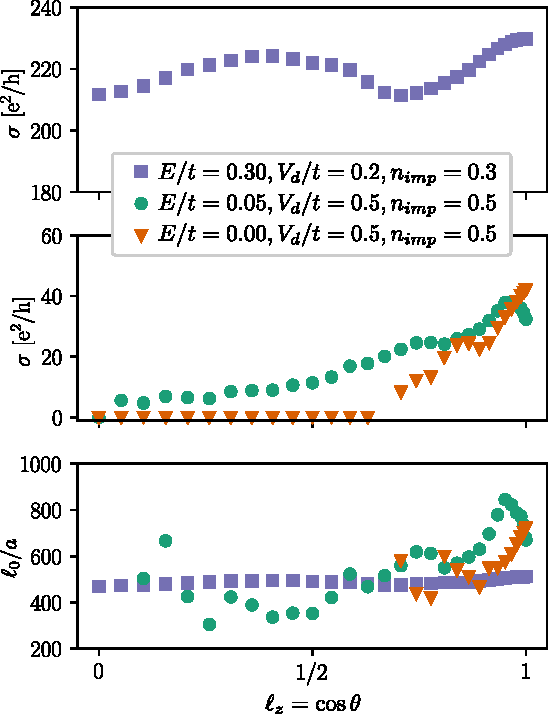
\includegraphics[width=\columnwidth]{{articles/sumit_paper/fig5.pdf}}}
\caption{The conductivity $\sigma$ and the mean free path $\ell_0$ in the symmetric coupling model of Eq.~(\ref{chap02:MODEL}) as the function of the N\'eel vector orientation $n_z=\cos\theta$. Both quantities are extracted from our numerical data with the help of  Eq.~(\ref{chap02:fit}). Large variations of the mean free path in the half-metal regime are associated with the Fermi energy touching the band edge at certain polar angles of the N\'eel vector.}
\label{chap02:fig:mfp}
\end{figure}
%%%%%%%%%

\section{Spin-orbit torques}

The package kwant \cite{groth_kwant:_2014} does not only provide the elements of the scattering matrix $S(E)$ in Eq.~(\ref{chap02:scattering}), but also gives access to the solutions $\Psi^{L,R}_{\alpha,E}(\bb{r})$ inside the sample. Such solutions can, therefore, be used to obtain a local expectation value of the electron spin (we refer here to the dimensionless spin defined by the operator $\bb{\sigma}/2$) as
\be
\label{chap02:sdensity}
\bb{s}(\bb{r})= \frac{1}{2}\int \frac{dE}{2\pi \hslash} \s_\textrm{A} f_A(E)  \sum_{\alpha}  \Psi^{A\;\dagger}_{\alpha,E} \bb{\sigma}_{\sigma\sigma'} \Psi^{A}_{\alpha,E}, 
 \e
where $\alpha=(n,\sigma,\nu)$ and the index $A=L,R$ numerates the leads. 

In order to extract spin-orbit torques we have to decompose the local electron spin to equilibrium and non-equilibrium contributions as
\be
\bb{s}(\bb{r})=\bb{s}_0(\bb{r})+\delta\bb{s}(\bb{r}).
\e
Equilibrium spin density, $\bb{s}_0$, corresponds to the limit of zero bias (or thermal bias) $f_L=f_R=f(E)$, where $f(E)$ is the Fermi-Dirac distribution function.  The quantity $\bb{s}_0$ describes equilibrium conduction electron contributions to the parameters of the Heisenberg model for localized momenta $\bb{S}_i$ that we do not discuss here. 

Non-equilibrium contribution, $\delta\bb{s}$, describes the effects induced e.\,g. by a bias voltage, $V_\textrm{bias}$, such as the spin-orbit torques on magnetization. In the linear response we obtain, in the spirit of Eq.~(\ref{chap02:Landauer}), the formula
\begin{align}
\frac{\delta\bb{s}(\bb{r})}{\delta\mu} =  \frac{1}{4h} \sum_{\alpha}  \lt[\Psi^{R\;\dagger}_{\alpha,E}(\bb{r}) \bb{\sigma}_{\sigma\sigma'} \Psi^{R}_{\alpha,E}(\bb{r}) \rt.  \lt. - \Psi^{L\;\dagger}_{\alpha,E}(\bb{r}) \bb{\sigma}_{\sigma\sigma'} \Psi^{L}_{\alpha,E}(\bb{r}) \rt],
\label{chap02:noneq}
\end{align}
where $\delta\mu=eV_\textrm{bias}$ and the scattering states are taken at the Fermi energy.  Similarly to Eq.~(\ref{chap02:Landauer}), we assume here that the quantities $\Psi^{A\;\dagger}_{\alpha,E} \,\bb{\sigma}\, \Psi^{A}_{\alpha,E}$  have negligible energy dependence within the interval $\delta\mu$ around the Fermi energy. 

In numerical simulations we systematically employ Eq.~(\ref{chap02:noneq}) to extract the spin density on $A$ and $B$ sublattices by varying the direction of the N\'eel vector. The results are fitted by the expansion of $\delta\bb{s}$ in angular harmonics that are compatible with the symmetry of the model. Before, we proceed with the discussion of our results let us pause to clarify the relation between the non-equilibrium spin-density and microscopic spin-orbit torques on magnetization that enter effective Landau-Lifshits-Gilbert (LLG) equation on magnetization dynamics.

\section{Microscopic LLG equation} 

The problem of magnetization dynamics can be formulated with the help of a Heisenberg model for the localized momenta $\bb{S}_i$ that is coupled to a tight-binding model for conduction electrons by means of the local exchange interaction of Eq.~(\ref{chap02:ex}). Depending on the type of the Heisenberg model we may obtain different equations of motion but the torques on magnetization (originating from electric current or field) and also Gilbert damping terms can be understood from the tight-binding Hamiltonian of Eq.~(\ref{chap02:MODEL}) alone \cite{ado_anisotropy_2019}. 

% For the sake of illustration let us outline the derivation of magnetization dynamics for a Heisenberg model of an ``isotropic'' antiferromagnet. The local interaction of Eq.~(\ref{chap02:ex}) dictates the equation of motion of localized momenta of the form
% \be
% \label{chap02:EOM}
% \dot{\bb{S}}_i = \bb{H}_i\times \bb{S}_i+ \frac{J}{\hslash}\, \bb{S}_i\times \s_{\sigma\sigma'} \lt\la c\h_{i\sigma}\bb{\sigma}_{\sigma\sigma'} c\0_{i\sigma'} \rt\ra,
% \e
% where dot stands for the time derivative of $\bb{S}_i$ and $\bb{H}_i=-\delta F/ \delta\, \hslash\bb{S}_i$ is an effective field (in frequency units) on a site $i$  that is defined by the free energy $F$ of the classical Heisenberg model for localized spins. The angular brackets denote the thermodynamic expectation value of conduction electron spin operator on the same site $i$. 

% For a collinear antiferromagnet we shall distinguish two sublattices $A$ and $B$ that are characterized by opposite directions of the localized momenta $\bb{S}_i^\textrm{A}=-\bb{S}_i^\textrm{B}$ in the antiferromagnetic ground state. It is assumed, that these directions remain to be almost opposite even for out-of-equilibrium conditions. It is also natural to assume that, as far as the magnet is far from a phase transition, the classical fields $\bb{S}_i^\textrm{A}$ and $\bb{S}_i^\textrm{B}$ remain smooth on atomic scales. Below we consider a single domain antiferromagnet, which is characterized by two time-dependent unit vectors $\bb{m}^\textrm{A,B}=\bb{S}^\textrm{A,B}/S$. 

% It is also convenient to define smooth conduction electron spin densities on each of the two sublattices
% \be
% \bb{s}^\textrm{A,B}(\bb{r})= \frac{1}{2} \s_{i\sigma\sigma'} \lt\la c\h_{i\sigma}\bb{\sigma}_{\sigma\sigma'} c\0_{i\sigma'} \rt\ra\;\frac{2}{\mathcal{A}},
% \e
% where $\mathcal{A}$ is the area of the unit cell (which naturally includes one A and one B site). Thus, the equation of motion (\ref{chap02:EOM}) can be written in  continuous approximation as
% \beml
% \label{chap02:EOMAFM}
% \begin{align}
% \dot{\bb{m}}^\textrm{A} &= \bb{H}^\textrm{A}\times \bb{m}^\textrm{A}+ (J\mathcal{A}/\hslash)\, \bb{m}^\textrm{A}\times \bb{s}^\textrm{A},\\
% \dot{\bb{m}}^\textrm{B}&= \bb{H}^\textrm{B}\times \bb{m}^\textrm{B}+ (J\mathcal{A}/\hslash)\, \bb{m}^\textrm{B}\times \bb{s}^\textrm{B},
% \end{align}
% \eml
% where $|\bb{m}^\textrm{A,B}|=1$, and the notations $\bb{H}^\textrm{A,B}$ refer to the effective fields on the sublattices $A$ and $B$. 

% Antiferromagnet dynamics is usually formulated as the coupled dynamics of the N\'eel and magnetization vectors,
% \be
% \bb{n}=\lt(\bb{m}^\textrm{A}-\bb{m}^\textrm{B}\rt)/2,\qquad \bb{m}= \lt(\bb{m}^\textrm{A}+\bb{m}^\textrm{B}\rt)/2,
% \e
% that remain mutually perpendicular $\bb{n}\cdot \bb{m}=0$ and yield the constraint $n^2+m^2=1$. Naturally, the amplitude of the magnetization vector remain to be small, $m\ll n \approx 1$.

% For an ``isotropic'' antiferromagnet, one finds the effective field \cite{gomonay_spintronics_2014} $\bb{H}^\textrm{A}+\bb{H}^\textrm{B}= J_\textrm{ex}\bb{m}/\hslash+2\bb{H}$, where $\bb{H}$ is an external magnetic field in frequency units and $J_\textrm{ex}$ is a direct antiferromagnetic exchange energy that is one of the largest energies in the problem. In turn, the combination $\bb{H}^\textrm{A}-\bb{H}^\textrm{B}$ is proportional to magnetic anisotropy that we choose not to take into account as mentioned above.  
The classical equations of motion on the staggered and non-staggered magnetizations, $\bb{n}$ and $\bb{m}$, were derived in Chapter~\ref{cd:sd:motion}. Excluding the anisotropy $K$, Eqs~(\ref{eq:sd:neel}) reads
\begin{align}
&\dot{\bb{n}} = -2\frac{J_\textrm{ex}}{\hslash} \bb{n}\times\bb{m} +\bb{H}\times\bb{n}+\frac{J\mathcal{A}}{\hslash}\lt(\bb{n}\times\bb{s}_++\bb{m}\times\bb{s}_-\rt),\n\\
&\dot{\bb{m}} = \bb{H}\times\bb{m}+\frac{J\mathcal{A}}{\hslash}\lt(\bb{m}\times\bb{s}_++\bb{n}\times\bb{s}_-\rt),
\label{chap02:AFMEOM}
\end{align}
where $\bb{s}_\pm=(\bb{s}_A\pm\bb{s}_B)/2$. The right-hand sides of Eqs.~(\ref{chap02:AFMEOM}) contain the quantities that can be called generalized torques. Here we are only interested in specific contributions to generalized torques that are induced by the chemical potential difference $\delta\mu=eV_\textrm{bias}$ between left and right leads. Such contributions define four spin-orbit torques  
\be
\label{chap02:SOT_def}
\bb{T}^\ell_\pm=(J\mathcal{A}/\hslash)\bb{n}\times\delta\bb{s}_\pm, \quad 
\bb{T}^m_\pm=(J\mathcal{A}/\hslash)\bb{m}\times\delta\bb{s}_\pm,
\e
where $\delta \bb{s}_\pm$ refers to the non-equilibrium spin density contribution that is proportional to $\delta\mu$. 

Note that, generally, the average spin $\bb{s}_i$ has a non-local functional dependence on the time-dependent classical field $\bb{S}_j$ at preceding moments of time  and at different lattice sites $j\neq i$. The degree of non-locality is defined by relaxation processes. The quicker the relaxation the more local the functional dependence. In particular, non-dissipative contributions to spin-orbit torques (the so-called field-like contributions) are local in time on the time scales of the order of $s$--$d$ exchange  $\tau_\textrm{sd}=\hslash/\Delta_\text{sd}$, where $\Delta_\text{sd}=J S$. In contrast, the dissipative contributions (such as anti-damping torques) are defined by transport scattering time $\tau_\textrm{tr}$. The latter time scale may be both larger and smaller than $\tau_\textrm{sd}$ giving rise to different regimes of magnetization dynamics. For the sake of numerical analysis we consider, however, a situation when these two time scales are of the same order.

\section{Symmetry consideration} 

Symmetry properties of spin-orbit torques and conductivity tensor can be understood from a low-energy approximation by projecting the model (\ref{chap02:ham}) on the states in a vicinity of $K$ points, 
\be
\bb{K}= \frac{4\pi}{3\sqrt{3} a}\bpm 1\\ 0\epm,\quad\mbox{and}\quad \bb{K}'= -\bb{K},
\e
as it is usually done for graphene. In the valley symmetric approximation we obtain the effective model
\be
\label{chap02:low}
H^\textrm{eff}_0= v\, \bb{p}\cdot\bb{\Sigma}+\alpha_\textrm{R}\lt[\bb{\sigma}\times\bb{\Sigma}\rt]_{\hat{z}} - \Delta_\text{sd}\,\bb{n}\cdot\bb{\sigma}\,\Sigma_z\Lambda_z,
\e
where $\bb{\Sigma}$, $\bb{\Lambda}$, and $\bb{\sigma}$ are the vectors of Pauli matrices in sublattice, valley and spin space, respectively, and 
\be
v= \frac{3}{2} t_h a/\hslash, \qquad \alpha_\textrm{R}= \frac{3}{2} \lambda , \qquad \Delta_\text{sd}=JS.
\e
Even though the model of Eq.~(\ref{chap02:ham}) is characterized by the point group $C_\textrm{3v}$, the effective low-energy model of Eq.~(\ref{chap02:low}) has a higher symmetry 
of the group $C_{\infty\textrm{v}}$. This is reflected by the fact that the Fermi-surfaces (for energies we are interested in) remain entirely isotropic irrespective of the N\'eel vector orientation as shown in Fig.~\ref{chap02:fig:lattice}. Moreover, the exact sublattice symmetry of the model, $\Lambda_x H^\textrm{eff}_0[-\bb{n}] \Lambda_x =H^\textrm{eff}_0[\bb{n}]$, ensures vanishing non-equilibrium staggered spin polarization $\delta \bb{s}_-=0$ irrespective of both the voltage bias and the N\'eel vector orientation. This property is indeed confirmed by the numerical analysis. 

The spin-orbit coupling term in Eq.~(\ref{chap02:low}) is proportional to the scalar product $\bb{\sigma}\cdot \lt[\hat{\bb{z}}\times \bb{v}\rt]$, where $\bb{v}=v\bb{\Sigma}$ is the velocity operator and $\hat{\bb{z}}$ is the unit vector in $z$ direction. In the presence of electric current $I$, which, in our model, is always directed along $x$ axis, the velocity operator averages to a non-zero value that is proportional to the current. One can see, therefore, that the second term in Eq.~(\ref{chap02:low}) can be interpreted as Zeeman coupling to an effective Rashba field $\hat{\bb{z}}\times \bb{I}$. Such a field induces non-equilibrium polarization $\delta\bb{s}_+$ in the same way as in ferromagnets. 

The symmetry of the point group $C_{\infty\textrm{v}}$ (see also the symmetry analysis in Refs.~\cite{vanderBijl2012, garello_symmetry_2013}) suggests that the tensor relation between non-equilibrium polarization $\delta\bb{s}_+$ and the Rashba field $\hat{\bb{z}}\times \bb{I}$ can be presented in a vector form as 
\begin{multline}
\delta\bb{s}_+\,= A_I(n_z^2)\,\hat{\bb{z}}\times \bb{I} + A'_I(n_z^2)\,\bb{n}_\parallel\times \lt[\bb{n}_\parallel\times \lt[\hat{\bb{z}}\times \bb{I}\rt]\rt]
+ B_\perp(n_z^2)\,\bb{n}_\perp\times \lt[\hat{\bb{z}}\times \bb{I}\rt]\\
+B_\parallel(n_z^2)\,\bb{n}_\parallel\times \lt[\hat{\bb{z}}\times \bb{I}\rt]+ C(n_z^2)\,\bb{n}_\parallel\times \lt[\bb{n}_\perp\times \lt[\hat{\bb{z}}\times \bb{I}\rt]\rt],
\label{chap02:symmetry}
\end{multline}
where we decompose the N\'eel vector $\bb{n}=\bb{n}_\parallel+\bb{n}_\perp$ into in-plane $\bb{n}_\parallel$ and perpendicular-to-the-plane $\bb{n}_\perp$ components. We parameterize $\bb{n}=(\cos\phi\sin\theta,\allowbreak \sin\phi\sin\theta, \allowbreak \cos\theta)^\top$, where $\theta$ is a polar angle and $\phi$ is an azimuthal angle. Consequently, we have $\bb{n}_\parallel=(\cos\phi\sin\theta,\sin\phi\sin\theta,0)^\top$ and $\bb{n}_\perp=(0,0,\cos\theta)^\top$.

The decomposition of Eq.~(\ref{chap02:symmetry}) is dictated by the symmetry analysis with respect to two transformations: the N\'eel vector inversion, $\bb{n}\to -\bb{n}$, and the N\'eel vector reflection, $\bb{n}_\perp\to -\bb{n}_\perp$, with respect to the electron 2D plane. 

Since the model (at the Fermi energies we choose) is isotropic with respect to in-plane rotations, these two symmetries are the only ones to characterize different contributions to non-equilibrium spin density. 

The first two terms in Eq.~(\ref{chap02:symmetry}) are even with respect to both the N\'eel vector inversion and the N\'eel vector reflection. The last term in Eq.~(\ref{chap02:symmetry}) is even with respect to the N\'eel vector inversion but odd with respect to the N\'eel vector reflection. These terms correspond to torques of the field-like symmetry, i.\,e. to the torques that are invariant under the time reversal operation. 

The second two terms in Eq.~(\ref{chap02:symmetry}), which are proportional to the coefficients $B_{\parallel,\perp}$, are odd with respect to the N\'eel vector reflection. The first one of them is odd while the second one is even with respect to the N\'eel vector reflection. These terms represent anti-damping spin-orbit torques that change sign under time reversal.

The coefficients in front of different vector forms in Eq.~(\ref{chap02:symmetry}) must remain invariant with respect to both symmetry transformations, but they may still vary as the function of the symmetry invariant $n_z^2$. The coefficients may also depend on $n^2$ but such dependence is absent within linear response approximation. Indeed, one shall take $n^2=1$ ($m=0$) in all coefficients in front of electric current since electric current is regarded as the only possible source of a deviation from the exact antiferromagnetic order. 

The exact sublattice symmetry of the symmetric coupling model of Eqs.~(\ref{chap02:ham})-(\ref{chap02:MODEL}) does not only ensure the vanishing staggered polarization $\delta\bb{s}_-=0$ but also leads to identically vanishing anti-damping torques $B_\parallel=B_\perp=0$ in all possible regimes. This is indeed confirmed by our numerical analysis for the symmetric coupling model as we describe below. 

%%%%%%%%%%%%
%%% figure 6: density
%%%%%%%%%%%%
\begin{figure}
\centering
\centerline{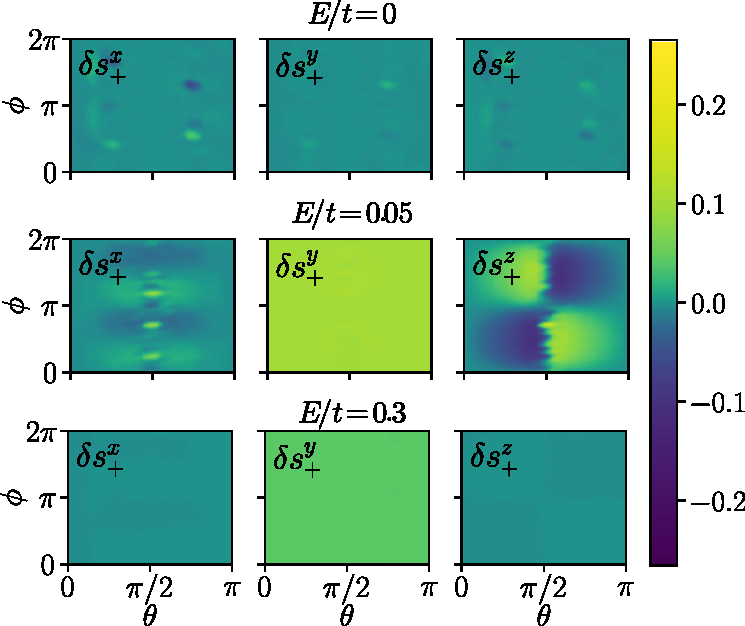
\includegraphics[width=\columnwidth]{{articles/sumit_paper/fig6.pdf}}}
\caption{Non-equilibrium spin density $\delta\bb{s}_+$ for the symmetric coupling model of Eqs.~(\ref{chap02:ham})-(\ref{chap02:MODEL}) with $V_\textrm{d}=0.5\,t_h$ as the function of the N\'eel-vector orientation for different values of the Fermi energy. Each data point foe each direction of the N\'eel vector corresponds to averaging over 30 impurity configurations. Spin densities are normalized to the scale $\Delta_\text{sd}\lambda j/evt_h^2$, where $j=I/W$ is the charge current density through the sample. Fluctuations at $\theta=\pi/4$ and $\theta=3\pi/4$ in the top panel and at $\theta=\pi/2$ in the middle panel are due to diverging mean free path for Fermi energy touching the bottom of the conduction band. The staggered spin density $\delta\bb{s}_-$ fluctuates around zero (not-shown). For $E/t_h=0$, the spin-density $\delta\bb{s}_+$ also fluctuates around zero as shown in the upper panel.}
\label{chap02:fig:density}
\end{figure}
%%%%%%%%%

\section{Results for symmetric model} 
\subsection{General}

With the help of the kwant package \cite{groth_kwant:_2014} we compute from Eq.~(\ref{chap02:noneq}) the mean spin density response $\delta\bb{s}/\delta\mu$ on both sublattices for various directions of the N\'eel vector $\bb{n}$ and three different Fermi energies. These results, which are presented in Fig.~\ref{chap02:fig:density}, have complex dependence on the orientation of the N\'eel vector. The dependence is, however, much simplified for non-equilibrium spin density response divided by the sample conductance. In other words, we observe that the non-equilibrium spin density has a much simpler form when expressed via the charge current density $\bb{j}=\bb{I}/W$ rather than via the bias voltage.

In all regimes considered we find $\delta\bb{s}_-=0$ and confirm the decomposition of Eq.~(\ref{chap02:symmetry}) with $B_\parallel=B_\perp=0$. Moreover, we also find that the coefficient $A_I(n_z^2)=A_I$ is constant, i.\,e. independent of the angle $\theta$ in all regimes we consider. In addition, we find that the non-equilibrium spin density vanishes identically, $\delta\bb{s}_+=\delta\bb{s}_-=0$ for $E=0$. This point corresponds to the exact electron-hole symmetry of the model, i.\,e. for $E=0$, the number of quasiparticles in the conduction and valence bands are exactly the same. 

Despite these general findings we still observe that the results for non-equilibrium spin density are qualitatively different in the metal and half-metal regimes. 

%%%%%%%%%%%%
%%% figure 7: decomposition
%%%%%%%%%%%%
\begin{figure}
\centering
\centerline{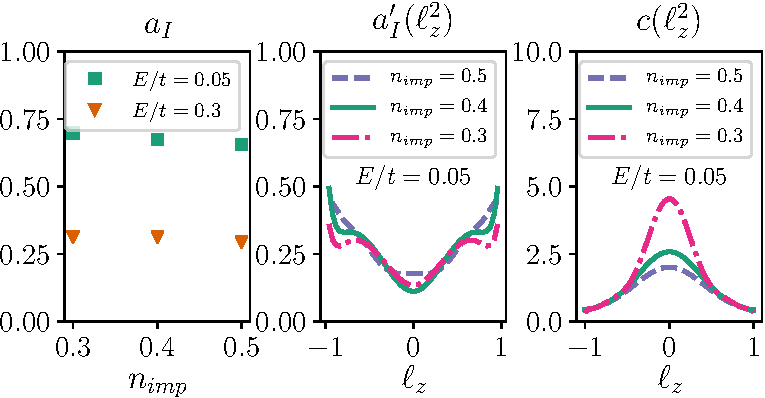
\includegraphics[width=\columnwidth]{{articles/sumit_paper/fig7.pdf}}}
\caption{The results of fitting simulation data for the symmetric coupling model with $L=2W=750\,a$ (partly shown in Fig.~\ref{chap02:fig:density}) with the ansatz of Eq.~(\ref{chap02:result1}). The data is obtained for $V_\textrm{d}=0.5\,t_h$. The data have been collected for 200 different orientations of the N\'eel vector for each impurity concentration.}
\label{chap02:fig:decomposition}
\end{figure}
%%%%%%%%%

\subsection{Metal regime}

The metal regime is characterized by two Fermi surfaces for each of the two valleys. This regime is represented in our simulations by the choice $E=0.3\,t_h$. In this case we also find $A'_I=C=0$ within our numerical accuracy. Thus, the metal regime in the symmetric model is represented by the only contribution to the non-equilibrium spin-density
\be
\label{chap02:s_SOT}
\delta\bb{s}_+= \frac{\Delta_\text{sd}\lambda}{2\pi evt_h^2} a_I\,\hat{\bb{z}}\times \bb{j}, 
\e
with a constant dimensionless coefficient $a_I$. This coefficient retains almost the same value for three different impurity concentrations as 
shown in the left panel of Fig.~\ref{chap02:fig:decomposition}. Thus, the non-equilibrium spin density in the metal regime is simply proportional to the Rashba field. The non-equilibrium spin density of Eq.~(\ref{chap02:s_SOT}) is readily recognized as the inverse spin-galvanic effect of Edelstein \cite{edelstein_spin_1990} that is widely known in ferromagnet materials with Rashba coupling \cite{manchon_theory_2008, garate_influence_2009}. 

Consequently, the spin orbit torques in the metal regime of the symmetric model are given solely by the isotropic Edelstein effect as
\be
\label{chap02:metal_SOT}
\bb{T}^\ell_+=a_I \eta\;\bb{n} \times\lt[\hat{\bb{z}}\times\bb{j}\rt],\quad
\bb{T}^m_+=a_I \eta\;\bb{m} \!\times\!\lt[\hat{\bb{z}}\times\bb{j}\rt], 
\e
where $\eta=J\mathcal{A}\Delta_\text{sd}\lambda /evh t_h^2$. 

This results of Eqs.~(\ref{chap02:s_SOT}), (\ref{chap02:metal_SOT}) are remarkably similar to those found analytically in the metal regime of a Rashba ferromagnet model with white-noise disorder \cite{ado_microscopic_2017,ado_anisotropy_2019}. The latter is also characterized by identically vanishing anti-damping spin-orbit torques and by a completely isotropic field-like torque of the same symmetry. Even though, analytical results have been obtained for a ferromagnet with a weak white-noise disorder, the same drastic simplification of the spin-orbit torque takes place for a symmetric honeycomb antiferromagnet with rather strong point-like disorder as demonstrated above. Such a simplification is, however, limited to the metal regime. 
 
\subsection{Half-metal regime} 
 
The half-metal regime is represented by the Fermi energy $E=0.05\,t_h$ that corresponds to the presence of a single Fermi surface in one of the valleys. The conductivity in this regime acquires strong dependence on $\theta$. In particular, for $n_z^2<1/2$, the system is poorly conducting as one can see already in the second panel of Fig.~\ref{chap02:fig:mfp}. Remarkably, we still find that the coefficient $A_I$ in Eq.~(\ref{chap02:symmetry}) is entirely independent of $\theta$ and anti-damping like torques are vanishing identically, $B_{\parallel,\perp}=0$. The coefficients $A'_I$ and $C$ are, however, finite and acquire some dependence on $n_z^2$.   

Thus, our numerical data in half-metal regime corresponds to the spin density
\begin{multline}
\label{chap02:result1}
\delta\bb{s}_+= \frac{\Delta_\text{sd}\lambda}{2\pi evt_h^2}
\Big(\,a_I\,\hat{\bb{z}}\times \bb{j} + a'_I(n_z^2)\,\bb{n}_\parallel\times \lt[\bb{n}_\parallel\times \lt[\hat{\bb{z}}\times\bb{j}\rt]\rt]\\
+c(n_z^2)\,\bb{n}_\parallel\times \lt[\bb{n}_\perp\times \lt[\hat{\bb{z}}\times\bb{j}\rt]\rt]\Big),
\end{multline}
where we also introduced the dimensionless functions $a'_I(n_z^2)$ and $c(n_z^2)$ that are shown in the middle and in the right panel of Fig.~\ref{chap02:fig:decomposition} for different impurity concentrations. 

The last two terms in Eq.~(\ref{chap02:result1}) represent high-harmonics field-like torques that are finite only in the half-metal regime. On symmetry grounds one should generally expect the field-like torques to be largely insensitive to disorder. Even though, the disorder dependence of $a_I$ and $a'_I$ coefficients is indeed negligible, the one of the function $c(n_z^2)$ is still rather strong for $n_z^2<1/2$. One should, however, remember that the coefficient $c$ is standing in front of the vector form that is vanishing for both $n_z=0$ and $n_z=\pm 1$, so the fit accuracy near these points is poor. Moreover, the case of almost in-plane N\'eel vector, $n_z^2\ll 1/2$, corresponds to the poorly conducting sample whose conductance is dominated by the variable range hopping processes due to strong disorder. Thus, we attribute this seemingly strong dependence of $c$ on disorder concentration to the mechanism of conduction. Still, the value of $c$ is found to be about 5 times larger than that of $a_I$ and about 10 times larger than that of $a'_I$, which makes the high-harmonic $c$-torque relevant in the half-metal regime. We note that the non-equilibrium spin density, which is proportional to $c(n_z^2)$, is directed perpendicular to the electron plane.  

Overall, the half-metal regime is characterized by the torques
\beml
\label{chap02:torque_T}
\begin{align}
\bb{T}^\ell_+=\eta \Big(\,&a_I\bb{n} \!\times\!\lt[\hat{\bb{z}}\!\times\!\bb{j}\rt] + 
a'_I(n_z^2)\, \bb{n}\!\times\!\lt[\bb{n}_\parallel\!\times\! \lt[\bb{n}_\parallel\!\times\! \lt[\hat{\bb{z}}\!\times\! \bb{j}\rt]\rt]\rt]\n\\
&\hspace{3cm}+c(n_z^2)\, \bb{n}\!\times\!\lt[\bb{n}_\parallel\!\times\! \lt[\bb{n}_\perp\!\times\! \lt[\hat{\bb{z}}\!\times\! \bb{j}\rt]\rt]\rt]\Big),
\label{chap02:torque_Tplus}\\
\bb{T}^m_+=\eta \Big(\,&a_I\bb{m} \!\times\!\lt[\hat{\bb{z}}\!\times\!\bb{j}\rt] + 
a'_I(n_z^2)\, \bb{m}\!\times\!\lt[\bb{n}_\parallel\!\times\! \lt[\bb{n}_\parallel\!\times\! \lt[\hat{\bb{z}}\!\times\! \bb{j}\rt]\rt]\rt]\n\\
&\hspace{3cm}+c(n_z^2)\, \bb{m}\!\times\!\lt[\bb{n}_\parallel\!\times\! \lt[\bb{n}_\perp\!\times\! \lt[\hat{\bb{z}}\!\times\! \bb{j}\rt]\rt]\rt]\Big),
\label{chap02:torque_Tminus}
\end{align}
\eml
where $\eta=J\mathcal{A}\Delta_\text{sd}\lambda /evh t_h^2$ is the same as in Eq.~(\ref{chap02:metal_SOT}). 

Note, that the function $a'_I(n_z^2)$ in Eq.~(\ref{chap02:torque_Tplus}) for $\bb{T}^\ell_+$ can be absorbed into the redefinition of the coefficients $a_I$ and $c$.  Indeed, with the help of a straightforward vector algebra one can re-write Eq.~(\ref{chap02:torque_Tplus}) as
\be
\label{chap02:torque_Tplus_MOD}
\bb{T}^\ell_+=\eta \Big(\tilde{a}_I(n_z^2)\bb{n} \!\times\!\lt[\hat{\bb{z}}\!\times\!\bb{j}\rt] 
+\tilde{c}(n_z^2)\, \bb{n}\!\times\!\lt[\bb{n}_\parallel\!\times\! \lt[\bb{n}_\perp\!\times\! \lt[\hat{\bb{z}}\!\times\! \bb{j}\rt]\rt]\rt]\Big),
\e
where we introduced
\be
\label{chap02:renorm}
\tilde{a}_I=a_I-(1-n_z^2)a'_I, \qquad \tilde{c}=c-a'_I.
\e
Thus, the modified coefficient $\tilde{a}_I$ acquires a weak dependence on $n_z^2$ due to a finite, though small, $a'_I$ contribution in the half-metal regime. 

To conclude this section it is worth mentioning that half-metal antiferromagnets are not entirely hypothetical. There have been several proposals in the past (see Refs.~\cite{van_leuken_half-metallic_1995, gong_electrically_2018} to name a few) and there has been also a recent material Mn$_2$Ru$_\textrm{x}$Ga that is recognized as a half-metal antiferromagnet \cite{kurt_cubic_2014, betto_zero-moment_2016}.

\section{Asymmetric coupling model} 

Relative simplicity of the results of Eqs.~(\ref{chap02:metal_SOT},\ref{chap02:torque_T}) for the symmetric coupling model of Eqs.~(\ref{chap02:ham})-(\ref{chap02:MODEL}) prompted us to look at a model with ultimately asymmetric $s$--$d$ exchange,
\be
H_\mathrm{sd}=\,-J \s_{i\in A }  \s_{\sigma\sigma'} \bb{\sigma}_{\sigma\sigma'}\bb{S}^\textrm{A}_i\cdot c^\dagger_{i\sigma}c\0_{i\sigma'},
\label{chap02:ex2}
\e
that is represented by $s$--$d$ coupling on $A$ sublattice only. Such a coupling obviously violates the sublattice symmetry and may, in principle, lead to the appearance of non-equilibrium staggered polarization and to anti-damping like spin-orbit torques that are absent in the symmetric coupling model. 

It is worth mentioning that the asymmetric model is unlikely to represent an antiferromagnet. Since conduction electron spins contribute to polarization only on a single sublattice, the model is much more likely to correspond to a ferrimagnet or a ferromagnet.  Rare-earth/transition metal ferrimagnets (such as FeCoGd) at a compensation point seem to be the most obvious examples \cite{jungfleisch_perspectives_2018}. The conduction electrons in these compounds couple mostly with localized d-orbitals rather than with f-orbitals and give rise to an asymmetric exchange coupling that can be mimicked by Eq.~(\ref{chap02:ex2}). 

In order to compute non-equilibrium spin-densities we repeat the analysis of the previous sections for the coupling of Eq.~(\ref{chap02:ex2}) that we refer to below as the asymmetric model. The band-structure of the asymmetric model is illustrated in Fig.~\ref{chap02:fig:BSas}. Similarly to the symmetric model we distinguish metal and half-metal regimes that are represented now by $E=0.3\,t_h$ and $E=0.1\,t_h$, correspondingly. 

The metal regime is characterized by two Fermi surfaces per valley, while the half-metal regime is characterized by a single Fermi surface per valley. The Fermi surfaces are illustrated in Fig.~\ref{chap02:fig:FSas} for $\theta=-\phi=\pi/4$, where $\theta$ and $\phi$ are now the polar and azimuthal angles of the unit vector $\bb{m}^\textrm{A}=(\cos\phi\sin\theta,\sin\phi\sin\theta,\cos\theta)^\top$, correspondingly. 

For numerical simulations we choose $\Delta_\text{sd}= J S=0.1\,t_h$, $\lambda=0.05\,t_h$, and $V_\textrm{d}=0.5\,t_h$ as for the symmetric model. 

Similarly to Eq.~(\ref{chap02:low}) the low energy sector of the asymmetric model is represented by the following effective Hamiltonian
\be
\label{chap02:low2}
H^\textrm{as}_0= v\, \bb{p}\cdot\bb{\Sigma}+\alpha_\textrm{R}\lt[\bb{\sigma}\times\bb{\Sigma}\rt]_{\hat{z}} - \frac{\Delta_\text{sd}}{2}\,\bb{m}^\textrm{A}\!\cdot\bb{\sigma}\,\lt(1+\Sigma_z\Lambda_z\rt),
\e 
that clearly lacks the sublattice symmetry. Interestingly, we observe from numerical simulations that the staggered non-equilibrium polarization $\delta \bb{s}_-$ is still vanishing in the metal regime, while it becomes finite in the half-metal regime. It has to be noted, however, that the separation to staggered and non-staggered polarization is largely irrelevant for the asymmetric model, since the latter is characterized by the only vector torque 
\be
\label{chap02:TA}
\bb{T}^\textrm{A}= \frac{J\mathcal{A}}{\hslash} \bb{m}^\textrm{A}\times\delta\bb{s}^\textrm{A}= \frac{J\mathcal{A}}{\hslash} \lt(\bb{n}+\bb{m}\rt)\times\lt(\delta\bb{s}_++\delta\bb{s}_-\rt),
\e
that is defined exclusively by the spin density on the sublattice A. 

%%%%%%%%%%%%
%%% figure 8: Band structure for asymmetric model
%%%%%%%%%%%%
\begin{figure}
\centering
\centerline{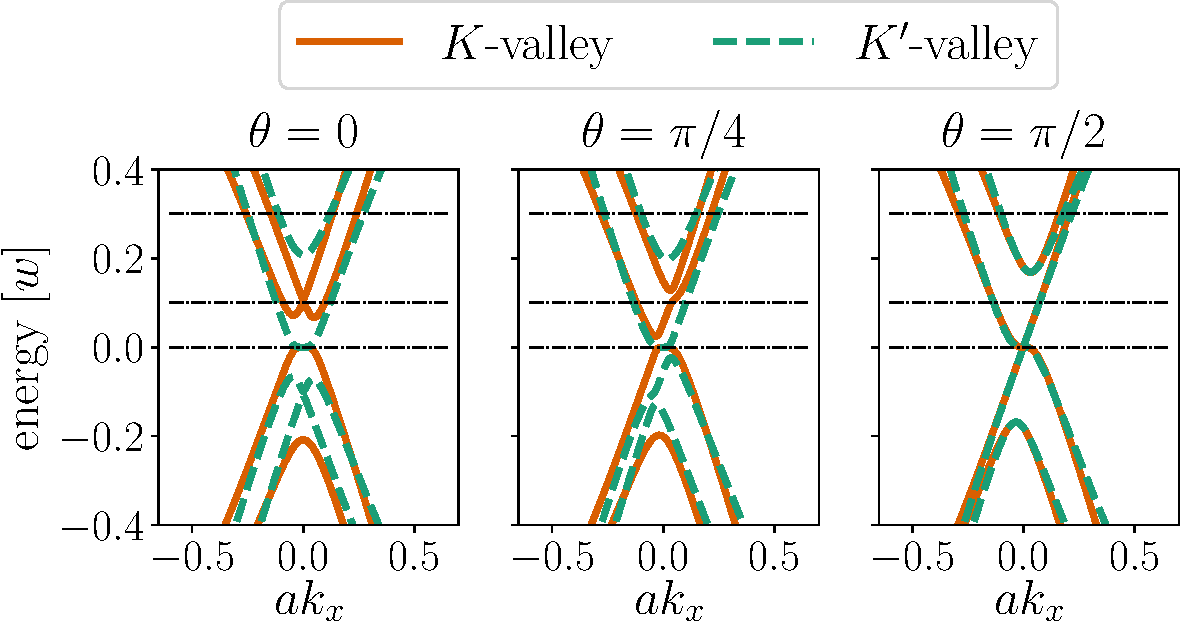
\includegraphics[width=\columnwidth]{{articles/sumit_paper/fig8.pdf}}}
\caption{Band structure for the asymmetric model. Dotted horizontal lines correspond to $E/t=0, 0.1$, and $0.3$.}
\label{chap02:fig:BSas}
\end{figure}
%%%%%%%%%

Indeed, for an ``isotropic'' antiferromagnet we find, in complete analogy with Eqs.~(\ref{chap02:AFMEOM}), the equations of motion
\beml
\label{chap02:AFMEOM2}
\begin{align}
&\dot{\bb{n}} = -2(J_\textrm{ex}/\hslash)\, \bb{n}\times\bb{m} +\bb{H}\times\bb{n}+\bb{T}^\textrm{A},\\
&\dot{\bb{m}} = \bb{H}\times\bb{m}+\bb{T}^\textrm{A},
\end{align}
\eml
which depend only on the spin-orbit torque $\bb{T}^\textrm{A}$. 

We would like to remind that the equations of motion of Eq.~(\ref{chap02:AFMEOM2}) are essentially incomplete since we do not investigate Gilbert-damping terms and we do not take into account anisotropy of antiferromagnet (as well as Dzyaloshinskii-Moriya interaction terms). The missing terms are essential if one wants to understand the magnetization dynamics, while they cannot alter the spin-orbit torque terms that we compute. 

%%%%%%%%%%%%
%%% figure 9: Fermi surfaces for asymmetric model
%%%%%%%%%%%%
\begin{figure}
\centering
\centerline{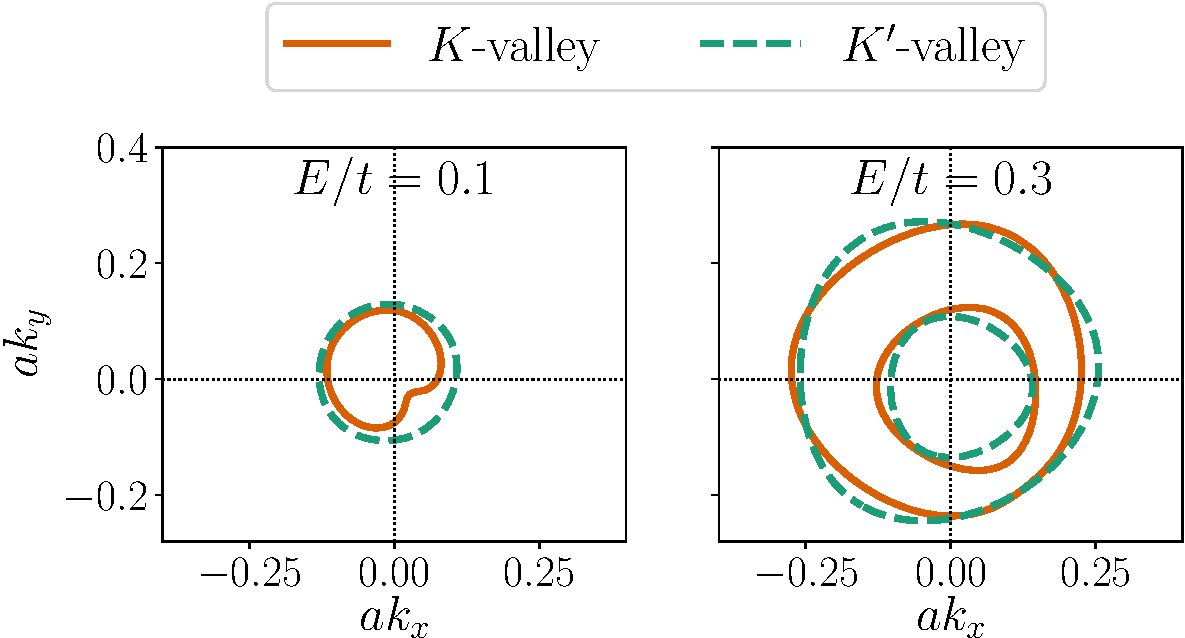
\includegraphics[width=\columnwidth]{{articles/sumit_paper/fig9.pdf}}}
\caption{The Fermi surfaces for the asymmetric model for the metal regime $E=0.3\,t_h$ (right panel) and the half-metal regime $E=0.1\,t_h$ (left panel). The Fermi surfaces are not round due to tridiagonal wrapping originating in $C_{3v}$ point-group symmetry of the crystal and due to in-plane component $\bb{m}^\textrm{A}_\parallel$ that affects the spectrum. The plots correspond to the choice $\theta=-\phi=\pi/4$. The momentum $\bb{k}$ is measured with respect to $\bb{K}$ point (solid lines) and $\bb{K}'$ point (dashed lines).}
\label{chap02:fig:FSas}
\end{figure}
%%%%%%%%%

As one can readily see from Fig.~\ref{chap02:fig:FSas}, the Fermi surfaces in the asymmetric model are not entirely round and reveal some tri-diagonal wrapping even for energies that are close to zero, $E\ll t_h$. The Fermi surfaces are also shifted with respect to the points $\bb{K}$ and $\bb{K}'$ and deformed depending on the azimuthal angle $\phi$ characterizing in-plane orientation of the vector $\bb{m}^\textrm{A}$. We find, however, that despite these effects the non-equilibrium spin-density $\delta\bb{s}^\textrm{A}$ can be very well decomposed using the symmetry analysis of the group $C_{\infty v}$ in analogy to Eq.~(\ref{chap02:symmetry}) for the symmetric coupling model. 

To do that we represent the vector $\bb{m}^\textrm{A}=\bb{m}_\parallel^\textrm{A}+\bb{m}_\perp^\textrm{A}$ as the sum of in-plane and perpendicular-to-the-plane components and decompose the numerical data with respect to the transformations: $\bb{m}_\perp^\textrm{A}\to -\bb{m}_\perp^\textrm{A}$ and $\bb{m}_\parallel^\textrm{A}=-\bb{m}_\parallel^\textrm{A}$. As the result, the non-equilibrium spin density (as the function of the vector components) is readily decomposed into the sum of four contributions,  
\be
\label{chap02:dec}
\delta\bb{s}^\textrm{A}[\bb{m}^\textrm{A}_\perp,\bb{m}^\textrm{A}_\parallel]= \delta\bb{s}_{++}+ \delta\bb{s}_{+-}+\delta\bb{s}_{-+}+\delta\bb{s}_{--},
\e
which are expressed as
\begin{multline}
\delta\bb{s}_{\zeta\kappa}=
\frac{1}{4}\Big(\delta\bb{s}^\textrm{A}[\bb{m}^\textrm{A}_\perp,\bb{m}^\textrm{A}_\parallel]+\zeta\, \delta\bb{s}^\textrm{A}[-\bb{m}^\textrm{A}_\perp,\bb{m}^\textrm{A}_\parallel]
+\kappa\, \delta\bb{s}^\textrm{A}[\bb{m}^\textrm{A}_\perp,-\bb{m}^\textrm{A}_\parallel]\\
+\zeta\kappa\, \delta\bb{s}^\textrm{A}[-\bb{m}^\textrm{A}_\perp,-\bb{m}^\textrm{A}_\parallel]\Big), 
\end{multline}
where $\zeta$ and $\kappa$ take on the values $\pm 1$. 

The bare results for non-equilibrium spin density $\delta\bb{s}^\textrm{A}$ (with a subtracted background component along $\bb{m}^\textrm{A}$) and the results for the contributions $\delta\bb{s}_{\zeta\kappa}$ are shown in Fig.~\ref{chap02:fig:density_as} for the metal regime, $E=0.3\,t_h$. Similar results are obtained for the half-metal regime, $E=0.1\,t_h$. 
 
%%%%%%%%%%%%
%%% figure 10: Density decomposition for asymmetric model
%%%%%%%%%%%%
\begin{figure}
\centering
\centerline{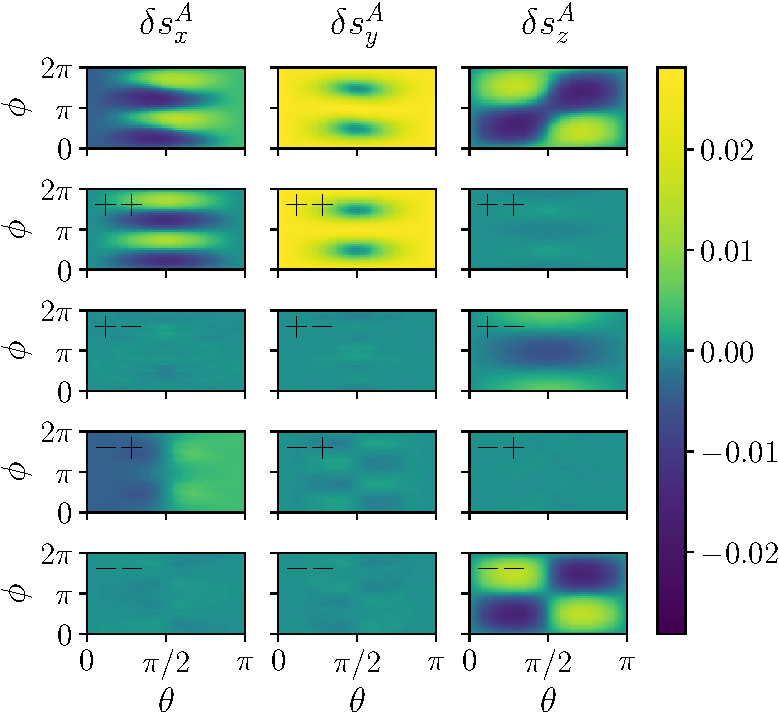
\includegraphics[width=\columnwidth]{{articles/sumit_paper/fig10.pdf}}}
\caption{Top panels show non-equilibrium spin density, $\delta\bb{s}^\textrm{A}$, for the asymmetric coupling model with subtracted background component along $\bb{m}^\textrm{A}$ in the units of $\Delta_\text{sd}\lambda j/evt_h^2$. The other panels represent the results of the spin-density decomposition of Eq.~(\ref{chap02:dec}). The results presented correspond to the ansatz of Eq.~(\ref{chap02:sA}). The data for density plots have been collected for 200 different orientations of the N\'eel vector for each impurity concentration. Each data point corresponds to averaging over at least 80 impurity configurations.}
\label{chap02:fig:density_as}
\end{figure}
%%%%%%%%%
 
We find that our numerical results for the non-equilibrium spin density $\delta\bb{s}^\textrm{A}$ (with subtracted background along $\bb{m}^\textrm{A}$ that does not enter the torque $\bb{T}^\textrm{A}$) are perfectly decomposed as a sum of five different vector forms in both metal and half-metal regimes,
\begin{align}
\delta\bb{s}^\textrm{A}&\,= A_I(n_z^2)\,\hat{\bb{z}}\times \bb{I} + A'_I(n_z^2)\,\bb{m}^\textrm{A}_\parallel\times \lt[\bb{m}^\textrm{A}_\parallel\times \lt[\hat{\bb{z}}\times \bb{I}\rt]\rt]\n\\
&+ B_\perp(n_z^2)\,\bb{m}^\textrm{A}_\perp\times \lt[\hat{\bb{z}}\times \bb{I}\rt]+B_\parallel(n_z^2)\,\bb{m}^\textrm{A}_\parallel\times \lt[\hat{\bb{z}}\times \bb{I}\rt]\n\\
&+C(n_z^2)\,\bb{m}^\textrm{A}_\parallel\times \lt[\bb{m}^\textrm{A}_\perp\times \lt[\hat{\bb{z}}\times \bb{I}\rt]\rt],
\label{chap02:sA}
\end{align}
where all coefficients are generally even functions of the component $n_z= n_z^\textrm{A}=\cos\theta$. Note that the first two vector forms are of the same symmetry with respect to both reflections $\bb{m}^\textrm{A}_\perp\to - \bb{m}^\textrm{A}_\perp$ and $\bb{m}^\textrm{A}_\parallel\to - \bb{m}^\textrm{A}_\parallel$.

%%%%%%%%%%%%
%%% figure 11: Results for asymmetric model
%%%%%%%%%%%%
\begin{figure}[t]
\centering
\centerline{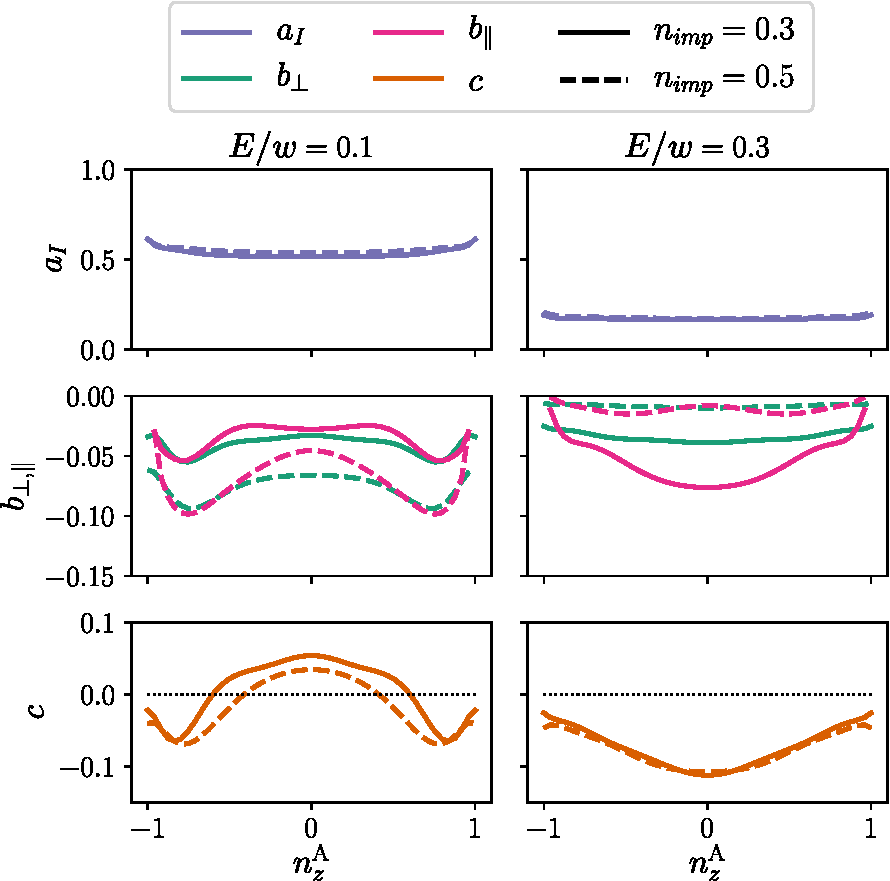
\includegraphics[width=\columnwidth]{{articles/sumit_paper/fig11.pdf}}}
\caption{Numerical results for the asymmetric coupling model that are expressed in the form of the angle dependent coefficients $a_I$, $b_\perp$, $b_\parallel$, and $c$ that define the spin-orbit torque $\bb{T}^\textrm{A}$ in Eq.~(\ref{chap02:TAresult}). The data is obtained by fitting the density data (partially represented in Fig.~\ref{chap02:fig:density_as}) using the ansatz of Eq.~(\ref{chap02:sA}).}
\label{chap02:fig:result_as}
\end{figure}

Remarkably, our numerical data again corresponds to a constant coefficient $A_I(n_z^2)=A_I$ in all regimes considered as it was also the case for the symmetric model.   

The spin orbit torque $\bb{T}^A$, which is obtained by substituting the result of Eq.~(\ref{chap02:sA}) to Eq.~(\ref{chap02:TAresult}), can be represented as the sum of only four vector forms 
\begin{align}
\bb{T}^\textrm{A}= \eta \Big(&a_I(n_z^2)\,\bb{m}^\textrm{A}\times\lt[\hat{\bb{z}}\times \bb{j}\rt] 
+ b_\perp(n_z^2)\,\bb{m}^\textrm{A}\times\lt[\bb{m}^\textrm{A}_\perp\times \lt[\hat{\bb{z}}\times \bb{j}\rt]\rt]\n\\
&+b_\parallel(n_z^2)\,\bb{m}^\textrm{A}\times\lt[\bb{m}^\textrm{A}_\parallel\times \lt[\hat{\bb{z}}\times \bb{j}\rt]\rt]\n\\
&+c(n_z^2)\,\bb{m}^\textrm{A}\times\lt[\bb{m}^\textrm{A}_\parallel\times \lt[\bb{m}^\textrm{A}_\perp\times \lt[\hat{\bb{z}}\times \bb{j}\rt]\rt]\rt]\Big),
\label{chap02:TAresult}
\end{align}
where we again introduce $\eta=J\mathcal{A}\Delta_\text{sd}\lambda /evh t_h^2$, $\bb{j}=\bb{I}/W$ and the dimensionless coefficients $a_I$, $b_\perp$, $b_\parallel$, and $c$ that all appear to be non-trivial functions of $n_z^2=\cos^2\theta$ as shown in Fig.~\ref{chap02:fig:result_as}. Note that the function $A'_I(n_z^2)$ in Eq.~(\ref{chap02:sA}) for spin density contributes to both $a_I$ and $c$ coefficients in Eq.~(\ref{chap02:TAresult}) in the direct analogy to Eqs.~(\ref{chap02:torque_Tplus_MOD}) and (\ref{chap02:renorm}). 

Thus, the spin-orbit torque $\bb{T}^\textrm{A}$ is parameterized by $4$ dimensionless functions. These functions are shown in Fig.~\ref{chap02:fig:result_as} illustrating the main result of our numerical simulations for the asymmetric coupling model. In sharp contrast to the symmetric model we observe that the anti-damping torques are no longer vanishing. We also find that $b_\perp(n_z^2) \approx b_\parallel(n_z^2)$ in the half-metal regime. The major field-like torque $\bb{m}^\textrm{A}\times\lt[\hat{\bb{z}}\times\bb{j}\rt]$, which originates in the Edelstein effect, acquires a weak dependence on $\theta$ due to the impact of the coefficient $A'_I(n_z^2)$. 

As it is expected we observe that anti-damping torques, which are proportional to $b_{\perp,\parallel}$, depend strongly on disorder concentration, while the field-like torques do not. Moreover, while anti-damping torques are suppressed by disorder in the metal regime, the opposite is true in the half-metal regime. 

Similarly to the symmetric model, the field-like torques are smaller in the metal regime than they are in half-metal regime. One can speculate, however, that anti-damping-like torques play a leading role in the metal regime of the asymmetric coupling model for sufficiently clean samples. We also see that anti-damping torques reveal rather strong anisotropy. In the metal regime they take on maximal values for in-plane orientations of the vector $\bb{m}^\textrm{A}$. 
 
It is also worth stressing that our results for asymmetric coupling model are the same for both ferromagnetic and antiferromagnetic order, since the spin-orbit torques are insensitive to the direction of the field $\bb{m}^\textrm{B}$.  

As have been already mentioned one can expect the asymmetric model to capture also the physics of layered ferrimagnets such as GdFeCo or Pt/GdFeCo \cite{jungfleisch_perspectives_2018, kim_spin-orbit_2018}. The magnetization switching by means of spin-orbit torques in these materials has recently become a subject of intense studies 
\cite{roschewsky_spin-orbit_2016, roschewsky_spin-orbit_2017, kim_spin-orbit_2018}.  In particular, the contribution from both field-like and anti-damping-like torques have been identified in GdFeCo films with perperndicular magnetocrystalline anisotropy in both transition-metal and rare-earth-metal rich configurations \cite{roschewsky_spin-orbit_2016, roschewsky_spin-orbit_2017}. 
These experimental results are, at least, qualitatively in line with our findings. 

%%%%
% figure 12
%
\begin{figure}[t]
\centering
\centerline{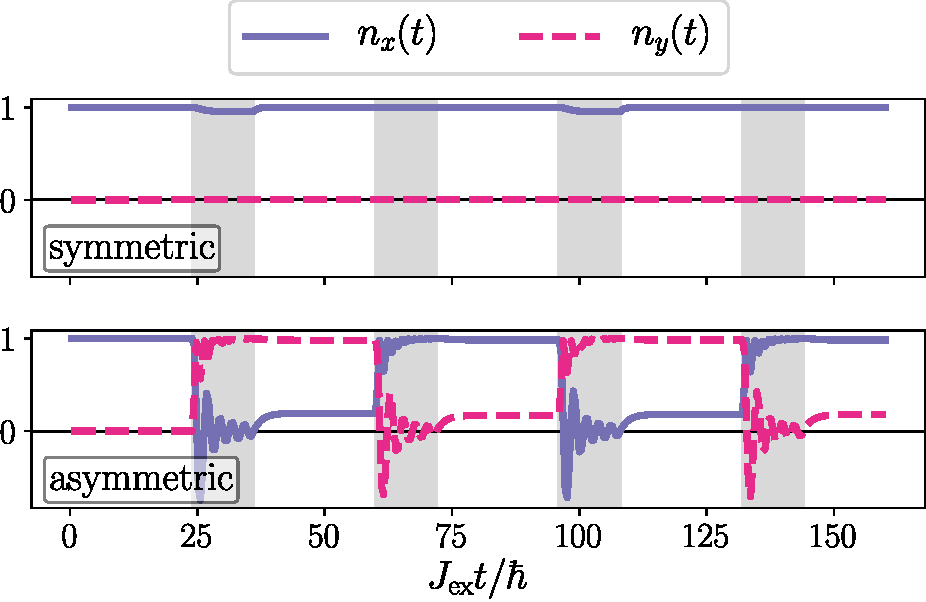
\includegraphics[width=\columnwidth]{{gfx/Chapter02/fig12}}}
\caption{Time evolution of the in-plane N\'eel vector $\bb{n}_\parallel(t)$ in the symmetric model (top panel) and asymmetric model (bottom panel) induced by a 
sequence of current pulses alternating between $-\hat{\bb{x}}$ and $\hat{\bb{y}}$ directions (gray areas). The results are obtained from Eqs.~(\ref{EOMAFM10}) for
 the parameters $\alpha=0.005$, $\hslash\eta j/J_\text{ex}=0.05$, $E/t_h=0.3$ and $n_\text{imp}=0.3$.}
\label{fig:switching}
\end{figure}

\section{Antiferromagnetic dynamics}

It is instructive to apply our results for the symmetric and asymmetric model to describe antiferromagnetic switching. As was mentioned in the introduction both field-like staggered torque and anti-damping-like non-staggered torque can be important for the N\'eel vector switching. In the symmetric model we only find field-like non-staggered torques that cannot induce AFM switching for realistic values of the current intensity. In the asymmetric model we find both field-like and anti-damping-like torques that act on a single sub-lattice. Although, strictly speaking, these do not entail a staggered torque, i.\,e. the N\'eel torque, one can nevertheless expect switching to occur. 

In order to model AFM magnetization dynamics we adopt the equations of motion (\ref{chap02:AFMEOM}) for the unit vectors $\bb{n}^\text{A}$ and $\bb{n}^\text{B}$  with Gilbert damping terms included,
\beml
\label{EOMAFM10}
\begin{align}
\dot{\bb{n}}^\text{A} &= 2\frac{J_\text{ex}}{\hslash}\bb{n}^\text{B}\times \bb{n}^\text{A}+ \frac{J\mathcal{A}}{\hslash}\, \bb{n}^\text{A}\times \bb{s}^\text{A} +\alpha\, \bb{n}^\text{A}\times \dot{\bb{n}}^\text{A},\\
\dot{\bb{n}}^\text{B}&= 2\frac{J_\text{ex}}{\hslash} \bb{n}^\text{A}\times \bb{n}^\text{B}+ \frac{J\mathcal{A}}{\hslash}\, \bb{n}^\text{B}\times \bb{s}^\text{B}+\alpha\, \bb{n}^\text{B}\times \dot{\bb{n}}^\text{B},
\end{align}
\eml
where we take $\alpha=0.005$ for the strength of the Gilbert damping.  

In Fig.~\ref{fig:switching} we illustrate the AFM dynamics induced by short current pulses of the density $j=0.05\,J_\text{ex}/\eta\hslash$, which are applied in alternating directions $-\hat{\bb{x}}$ and $\hat{\bb{y}}$. The parameters of spin-orbit torques are derived for the Fermi energy $E =0.3\,t_h$ (in the metal regime) and for the impurity concentration $n_\text{imp}=0.3$ which corresponds to placing impurities on $30\%$ of lattice sites.   

The spin-orbit torques in the symmetric model are obtained by substituting $\bb{s}^\text{A}=\bb{s}^\text{B} = \delta\bb{s}_+$ in Eqs.~(\ref{EOMAFM10}), where $\delta\bb{s}_+ \propto \hat{\bb{z}}\times\bb{j}$ is given by Eq.~(\ref{chap02:s_SOT}). The spin-orbit torques in the asymmetric model correspond to $\bb{s}^\text{B}=0$ and $\bb{s}^\text{A}$ taken from Eq.~(\ref{chap02:sA}).
 
It is worth noting that the switching behaviour in the asymmetric model (shown in the bottom panel of Fig.~\ref{fig:switching}) is provided exclusively by the field-like-torques (which are proportional to the $a_I$ and $c$ in Eq.~(\ref{chap02:TAresult})). In contrast, anti-damping torques, which are proportional to $b_{\perp,\parallel}$, do not play an important role in this behaviour for the proposed choice of parameters. Nevertheless, if anti-damping torques become essentially enhanced to overcome Gilbert damping they may lead to qualitatively different behaviour. Indeed, for giant anti-damping torques, the spin angular momentum in the asymmetric model is transferred from one sub-lattice to the another. Such a process, however, destroys the N\'eel order and fully magnetizes the sample during the current pulse. Once the electric current is switched off the N\'eel order is restored albeit in a different direction. This type of switching bears some resemblance to all-optical ultra-fast magnetization switching that is observed, for example, in a ferrimagnet GdFeCo \cite{RevModPhys.82.2731}. In the latter case the crystal also enters a transient fully magnetized state during a femtosecond optical pulse and relaxes to a state with opposite magnetization soon after the pulse.  We note however, that a current-induced switching of this type in our AFM model would require unrealistically large charge current intensities due to rather small magnitude of anti-damping torques. 

\section{Conclusions}
 
Motivated by recent experiments on the N\'eel vector switching we investigate microscopically the spin-orbit torques in an $s$--$d$-like model of a two-dimensional honeycomb antiferromagnet with Rashba spin-orbit coupling. We investigated the model with preserved and broken sublattice symmetry and distinguished metal and half-metal regimes for each of the model. Spin-orbit interaction in combination with on-site disorder potential and local exchange coupling between conduction and localized spins have been responsible for a microscopic mechanism of the angular momentum relaxation. We find identically vanishing anti-damping and N\'eel spin-orbit torques in the symmetric model in all regimes considered. As the result, the metal regime of the symmetric model is characterized by a particularly simple isotropic field-like spin-orbit torque, while the half-metal regime is characterized by anisotropic spin-orbit torques of the field-like symmetry.  Finite and anisotropic anti-damping torques, that crucially depend on disorder strength, are found in both metal and half-metal regimes of the asymmetric model. We also find non-equilibrium staggered polarization in the half-metal regime of the asymmetric model. This formally leads to a finite value of the N\'eel spin-orbit torque, which is, however, not a quantity of interest in that model. Overall, our results reveal the importance of two-dimensional electron momentum confinement for spin-orbit torque anisotropy. Largest values of spin-orbit torques are also associated with the half-metal regimes of conduction in both models.  % Numerical approach to calculating Spin-orbit torques
\cleardoublepage
\addtocontents{toc}{\protect\vspace{\beforebibskip}}%

%************************************************
\chapter{Gilbert damping in Rashba honeycomb antiferromagnets} % $\mathbb{ZNR}$
%************************************************
Giant Gilbert damping anisotropy is identified as a signature of strong Rashba spin-orbit coupling in a two-dimensional antiferromagnet on a honeycomb lattice. The phenomenon originates in spin-orbit induced splitting of conduction electron subbands that strongly suppresses certain spin-flip processes. As a result, the spin-orbit interaction is shown to support an undamped non-equilibrium dynamical mode that corresponds to an ultrafast in-plane N\'eel vector precession and a constant perpendicular-to-the-plane magnetization. The phenomenon is illustrated on the basis of a two dimensional $s$-$d$ like model. Spin-orbit torques and conductivity are also computed microscopically for this model. Unlike Gilbert damping these quantities are shown to reveal only a weak anisotropy that is limited to the semiconductor regime corresponding to the Fermi energy staying in a close vicinity of antiferromagnetic gap.

\vfill
bla bla
\clearpage

\section{Introduction}

A gapless character of the spin-wave spectrum in isotropic Heisenberg magnets in two dimensions results in the homogeneity of magnetic ordering being destroyed by thermal fluctuations at any finite temperatures. In contrast, in van der Waals magnets, characterized by intrinsic magnetocrystalline anisotropy that stems from spin-orbit coupling \cite{Lado2017}, an ordered magnetic state can be retained down to a monolayer limit. Two-dimensional (2D) van der Waals magnets are currently experiencing a revived attention \cite{Gong2017,Herrero2017,Burch2018,Tokmachev2018,Gong2019,Novoselov2019,Cortie2019} driven by the prospects of gateable magnetism \cite{Huang2018,Shengwei2018,Wang2018,Deng2018}, a continuing search for Kitaev materials \cite{Nagler2019,Gordon2019} and Majorana fermions \cite{Livanas2019}, topologically driven phenomena \cite{Mokrousov2019} as well as various applications \cite{Herrero2017,Burch2018,Novoselov2019}. The trade-off between quantum confinement, nontrivial topology and long-range magnetic correlations determines their unique magnetoelectronic properties, in particular a tunable tunneling conductance \cite{Wang2018a} and magnetoresistance \cite{Song2018,Klein2018,Kim2018} depending on the number of layers in the sample, as well as long-distance magnon transport \cite{Xing2019}. 

Ferromagnetic thin films have already entered commercial use in hard drives, magnetic field and rotation angle sensors and in similar devices  \cite{Parkin2003,Jogschies2015,Novoselov2019}, while keeping high promises for technologically competitive ultrafast memory elements \cite{Lau2016} and neuromorphic chips \cite{Fukami2016}. Moreover, it has recently been suggested that current technology may have a lot to gain from antiferromagnet (AFM) materials. Indeed, manipulating AFM domains does not induce stray fields and has no fundamental speed limitations up to THz frequencies \cite{Jungwirth2016AFMreview}. Despite their ubiquitousness, AFM materials have, however, avoided much attention from technology due to an apparent lack of control over the AFM order parameter -- the N\'eel vector. Switching the N\'eel vector orientation by short electric pulses has been put forward only recently as the basis for AFM spintronics \cite{MacDonald2011,Gomonay2014,Zelezny2014}. The proposed phenomenon has been soon observed in non-centrosymmetric crystals such as CuMnAs \cite{Wadley2016, Fina2016, Zelezny2018, Saidl2017} and Mn$_2$Au \cite{Barthem2013, Jordan2015, Bhattacharjee2018}. It should be noted that in most cases AFMs are characterized by insulating type behavior \cite{Pandey2017}, limiting the range of their potential applications, e.g., for spin injection \cite{Tshitoyan2015}. Interestingly, antiferromagnetic Mn$_2$Au possesses a typical metal properties, inheriting strong spin-orbit coupling and high conductivity, and is characterized by collective modes excitations in THz range \cite{Bhattacharjee2018}.

Despite a lack of clarity concerning the microscopic mechanisms of the N\'eel vector switching, these experiments have been widely regarded as a breakthrough in the emerging field of THz spintronics \cite{Bhattacharjee2018, Gomonay2016AFM, Olejnik2018, Jungwirth2018, Wadley2016, Jungwirth2016AFMreview, Baltz2018, Jungwirth2018, Hoffman2018}. It has been suggested that current-induced N\'eel vector dynamics in an AFM is driven primarily by the so-called N\'eel spin-orbit torques \cite{Brataas2012, Hals2013, Zelezny2014, 2014MokrousovSOT, Ghosh2017, SmejkalAFM_2017, Zelezny2018, Zhou2018, Manchon2018, Moriyama2018, Li2019, Chen2019, Zhou2019, Zhou2019a, Bodnar2018}. The N\'eel spin-orbit torque originates in a non-equilibrium staggered polarization of conduction electrons on AFM sublattices \cite{Zelezny2014, SmejkalAFM_2017, Zelezny2018, Manchon2018}. Characteristic magnitude of the non-equilibrium staggered polarization and its relevance for the experiments with CuMnAs and Mn$_2$Au remain, however, debated. 

The N\'eel vector dynamics in an AFM is also strongly affected by an interplay between different types of Gilbert dampings. Unlike in a simple single-domain ferromagnet with a single sublattice, the Gilbert damping in an AFM is generally different on different sublattices and includes spin pumping from one sublattice to another. A proper understanding of Gilbert damping is of key importance for addressing not only the mechanism of spin pumping but also domain wall motion, magnon lifetime, AFM resonance width and many other related phenomena \cite{PhysRevMaterials.1.061401, Kamra2018, Mahfouzi2018a, Yuan_2019, Hals2011}. It is also worth noting that spin pumping between two thin ferromagnetic layers with antiparallel magnetic orientations share many similarities with Gilbert damping in a bipartite AFM \cite{Heinrich2003,Tserkovnyak2005}. 

A conduction electron mechanism for Gilbert damping in collinear ferromagnet requires some spin-orbit interaction to be present. It is, therefore, commonly assumed that spin-orbit interaction of electrons naturally enhances the Gilbert damping. Contrary to this intuition, we show that Rashba spin-orbit coupling does generally suppress one of the Gilbert damping coefficients and leads to the appearance of undamped non-equilibrium N\'eel vector precession modes in the AFM. 

%%%%%%%%%%%%
%%% figure 1: lattice
%%%%%%%%%%%%
\begin{figure}
\centering
\centerline{\includegraphics[width=\columnwidth]{{articles/misha_paper/fig1.pdf}}}
\caption{A model of Rashba honeycomb antiferromagnet with two sublattices, $A$ and $B$, and on-site exchange interaction between localized momenta and conduction electrons (see Eq.~\ref{chap03:ex}). The large blue arrow represents the N\'eel vector vector, $\bm{n}$, that is in general, characterized by non-vanishing in-plane, $\bm{n}_\parallel$, and perpendicular-to-the-plane, $\bm{n}_\perp$, components. We refer to a specific coordinate system with $\hat{\bm{x}}$ axis chosen to be in the direction of $\bm{n}_\parallel$. 
}
\label{chap03:fig:lattice}
\end{figure}
%%%%%%%%%

Spin dynamics in a bipartite AFM is described in terms of two mutually orthogonal vector fields, namely the vector $\bb{n}(t)$ that is proportional to the N\'eel vector (difference between sublattice moments) and the vector $\bb{m}(t)$ that is proportional to the net magnetization (sum of sublattice moments) of a sample. Even though the AFM ground state corresponds to $\bb{m}=0$, it is widely understood that no N\'eel dynamics is possible without formation of a small but finite nonequilibrium magnetization $\bb{m}$. It appears, however, that Gilbert damping terms associated with the time dynamics of $\bb{m}(t)$ and $\bb{n}(t)$ are essentially different from a microscopic point of view.   

Indeed, the Gilbert damping that is proportional to $\partial_t\bb{n}$ is characterized by a coefficient $\alpha_n$, which is vanishing in the absence of spin-orbit interaction, much like it is the case in the ferromagnets. This behavior can be traced back to a spin-rotational symmetry of the collinear AFM. Indeed, the absolute value of $\bb{n}$ is conserved up to the order $m^2$. Thus, the dynamics of the N\'eel vector is essentially a rotation that does not change the conduction electron spectrum as far as the spin-rotation invariance is present. Breaking the spin-rotation symmetry by spin-orbit interaction induces, therefore, a finite $\alpha_n$, which is quadratic with respect to spin-orbit interaction strength.

In contrast, the Gilbert damping that is proportional to $\partial_t\bb{m}$ originates directly in the conduction electron scattering even in the absence of any spin-orbit interaction. The strength of the damping in a simple symmetric AFM is characterized by a coefficient $\alpha_m$, which is typically much larger than $\alpha_n$. As a rule, the spin-orbit interaction tends to suppress the coefficient $\alpha_m$ by restricting the ways in which electrons can damp their magnetic moments.  The condition $\alpha_m \gg \alpha_n$ has been indeed well documented in a metallic AFM \cite{PhysRevMaterials.1.061401, Mahfouzi2018a}. 

In this paper, we uncover the microscopic mechanism of strong and anisotropic Gilbert damping suppression due to the influence of spin-orbit interaction in a 2D AFM model on a honeycomb lattice. 

Below we focus mainly on the AFM in the regime of good metallic behavior, such that the Fermi energy of electrons exceeds by order of magnitude that of an effective $s$-$d$ exchange coupling between electron spins and localized AFM magnetic momenta.  In this case, the transition to the highly anisotropic regime takes place provided the characteristic spin-orbit energy $\lambda$ exceeds the scale $\hslash/\tau$, where $\tau$ is the electron scattering time. Alternatively, one may think of characteristic spin-orbit length becoming smaller than the mean free path of conduction electrons.  We show here that the splitting of 2D Fermi surfaces by spin-orbit interaction leads to a dramatic suppression of electron spin flips in certain directions. This results in a strong anisotropy of both Gilbert damping tensors $\hat{\alpha}_n$ and $\hat{\alpha}_m$, that get some of their principal components vanishing. This extreme anisotropy in the damping leads to essentially undamped N\'eel vector dynamics for certain nonequilibrium modes. 

In particular, we identify a specific undamped mode that corresponds to perpendicular-to-the-plane magnetization $\bb{m} \propto \hat{\bb{z}}$ and in-plane N\'eel vector $\bb{n}(t) \perp \hat{\bb{z}}$. The N\'eel vector corresponding to the mode has a precission around $\bb{m}$ with the frequency $J_\textrm{ex} m/\hslash$, where $J_\textrm{ex}$ is the value of the isotropic AFM exchange.

The presence of the undamped mode identified here, illustrates how lowering the symmetry of the electronic bath (by spin-orbit interaction) may induce a conservation law in the localized spin subsystem. Based on this microscopic mechanism we provide qualitative arguments in favor of a generality of the giant Gilbert damping anisotropy in a 2D metalic AFM with spin-orbit coupling. Even though the undamped mode cannot be associated with a single spin-wave or a magnon, its presence has a strong impact on the nonequilibrium N\'eel vector dynamics in 2D Rashba AFMs.

Apart from the Gilbert damping our results extend to cover conductivity and spin-orbit torques in the Rashba honeycomb AFM model. We also demonstrate how weak anisotropy of all these quantities emerge with Fermi energies approaching the AFM band gap. 

\section{Phenomenology of AFM dynamics}

In this paper, we choose to describe the AFM with a classical Heisenberg model for localized spins $\bb{S}^\textrm{X}= S \bb{n}^\textrm{X}$ on two sublattices $X=A,B$. The spins have the same modulus $S$ and antiparallel directions $\bb{n}^\textrm{A}=-\bb{n}^\textrm{B}$ in the ground state. The AFM Heisenberg model is coupled to an effective tight-binding model of conduction electrons (see Appendix~\ref{chap03:sec:appa}) by means of exchange interaction,
\be
\label{chap03:ex}
H_\mathrm{sd}=-J \s_{i} \s_{\sigma\sigma'}\bb{S}_i\cdot \bb{\sigma}_{\sigma\sigma'}c^\dagger_{i\sigma}c\0_{i\sigma'},
\e
where $J$ stands for an $s$-$d$-like exchange energy that is the same on $A$ and $B$ sublattices, the operators $c\h_{i\sigma}$ ($c\0_{i\sigma}$) are the standard creation (annihilation) operators for an electron on the lattice site $i$ with the spin index $\sigma$, and the notation $\bb{\sigma}=(\sigma_x,\sigma_y,\sigma_z)$ represents the three-dimensional vector of Pauli matrices. 

The real-time dynamics of AFM is, then, defined by two coupled differential equations (Landau-Lifshitz-Gilbert equations) on the unit vectors $\bb{n}^\textrm{A}$ and $\bb{n}^\textrm{B}$, 
\beml
\label{chap03:basicEQ}
\begin{align}
\dot{\bb{n}}^\textrm{A} &= \bb{H}^\textrm{A}\times\bb{n}^\textrm{A}  + (J\mathcal{A}/\hslash)\,\bb{n}^\textrm{A}\times \bb{s}^\textrm{A},\\
\dot{\bb{n}}^\textrm{B}&= \bb{H}^\textrm{B}\times\bb{n}^\textrm{B} +(J\mathcal{A}/\hslash)\,\bb{n}^\textrm{B}\times \bb{s}^\textrm{B},
\end{align}
\eml
where dot stands for the time derivative, $\bb{s}^\textrm{X}$ is the spin density of conduction electrons on the sublattice $X$,
\be
\bb{s}^\textrm{A,B}(\bb{r})= \frac{1}{2} \s_{i\sigma\sigma'} \lt\la c\h_{i\sigma}\bb{\sigma}_{\sigma\sigma'} c\0_{i\sigma'} \rt\ra\;\frac{2}{\mathcal{A}},
\e
and $\mathcal{A}$ is the area of the unit cell in the AFM. The notations $\bb{H}^\textrm{A,B}$ refer to effective fields on the sublattices $A$ and $B$ that are defined by the Heisenberg model. 

For an isotropic antiferromagnet, one finds an effective field \cite{Gomonay2014} $\bb{H}^\textrm{A}+\bb{H}^\textrm{B}= J_\textrm{ex}\bb{m}/\hslash+2\bb{H}$, where $\bb{H}$ is an external magnetic field in frequency units and $J_\textrm{ex}$ is a direct antiferromagnetic exchange energy that is one of the largest energies in the problem. In turn, the combination $\bb{H}^\textrm{A}-\bb{H}^\textrm{B}$ is proportional to magnetic anisotropy that we do not specify in this paper.  

Magnetization dynamics in AFM is conveniently formulated in terms of the N\'eel and magnetization vectors,
\be
\bb{n}=\lt(\bb{n}^\textrm{A}-\bb{n}^\textrm{B}\rt)/2,\qquad \bb{m}= \lt(\bb{n}^\textrm{A}+\bb{n}^\textrm{B}\rt)/2,
\e
that remain mutually perpendicular $\bb{n}\cdot \bb{m}=0$ and yield the constraint $n^2+m^2=1$. The dynamics necessarily induces a finite nonequilibrium magnetization vector $\bb{m}$, while the condition $m\ll 1$ remains to be fulfilled.  

From Eqs.~(\ref{chap03:basicEQ}) we obtain
\beml
\label{chap03:AFMEOM}
\begin{align}
\label{chap03:ndot}
\dot{\bb{n}} &= -\Omega\, \bb{n}\times\bb{m} +\bb{H}\times\bb{n}+\bb{n}\times\bb{s}^++\bb{m}\times\bb{s}^-,\\
\label{chap03:mdot}
\dot{\bb{m}} &= \bb{H}\times\bb{m}+\bb{m}\times\bb{s}^++\bb{n}\times\bb{s}^-,
\end{align}
\eml
where $\Omega=2J_\textrm{ex}S/\hslash$ and $\bb{s}^{\pm}= J \mathcal{A}\,(\bb{s}^\textrm{A}\pm\bb{s}^\textrm{B})/2\hslash$. In Eqs.~(\ref{chap03:AFMEOM}) we have deliberately skipped terms that are induced by anisotropy of AFM exchange since the latter depend on particularities of the AFM Heisenberg model that we do not discuss here.  

The vector $\bb{s}^+$ is proportional to average polarization of conduction electrons, while the vector $\bb{s}^-$ is proportional to the staggered polarization. The quantities $\bb{s}^\pm=\bb{s}_0^\pm+\delta\bb{s}^\pm$ contain equilibrium contributions $\bb{s}_0^\pm$ that characterize various interactions induced by conduction electrons. These contributions do renormalize the parameters of the AFM Heisenberg model and are not the subject of the present paper. 

%%%%%%%%%%%%
%%% figure 2: spectrum
%%%%%%%%%%%%
\begin{figure}
\centering
\centerline{\includegraphics[width=\columnwidth]{{articles/misha_paper/fig2.pdf}}}
\caption{Electronic band structure of the honeycomb AFM model of Eq.~(\ref{chap03:eff}) for different orientations of the N\'eel vector ($n_z=\cos\theta$). Two-dimensional momenta $\bb{p}$ are measured with respect to the wave-vectors $\bm{K}$ and $\bm{K}^\prime$ that specify two nonequivalent valleys. Deviation of the N\'eel vector from the perpendicular-to-the plane configuration ($\theta=0$) lifts the valley degeneracy. We restrict our analysis to the metallic regime with Fermi energies corresponding to two Fermi surfaces per valley (an example is shown by a black dotted line). The energy scale $\Delta$ characterizes the strength of $s$-$d$ exchange interaction.
}
\label{chap03:fig:spectrum}
\end{figure}
%%%%%%%%%

The nonequilibrium contributions $\delta\bb{s}^{\pm}$ originate from various forces applied to conduction electrons. One natural example is the electric field that not only induces an electric current in the sample but also contributes to $\delta\bb{s}^{\pm}$. The electric field can be further related to electric current by the resistivity tensor. The response of spin densities to electric current defines the so-called spin-orbit torques in Eqs.~(\ref{chap03:AFMEOM}) that we also compute.

Similarly, the response of $\delta\bb{s}^{\pm}$ to the time derivatives $\dot{\bb{n}}$ and $\dot{\bb{m}}$ describe various types of Gilbert damping induced by conduction electrons. Quite generally, such a response can be written in the form of a tensor
\be
\label{chap03:response}
\bpm 
\delta \bb{s}^{+}\\
\delta \bb{s}^{-}
\epm=
\bpm 
\hat{\alpha}_m & \hat{\alpha}_{mn}\\
\hat{\alpha}_{nm} & \hat{\alpha}_n
\epm
\bpm 
\dot{\bb{m}}\\
\dot{\bb{n}}
\epm,
\e
where all tensor components may themselves depend on the vectors $\bb{n}$ and $\bb{m}$. 

Gilbert dampings, in their original meaning, correspond to the contributions to $\delta\bb{s}^{\pm}$ that are symmetric under the time reversion. 
The terms that change sign should, more appropriately, be referred to as effective spin renormalizations. Both types of terms are, however, obtained from the microscopic analysis of the Gilbert damping tensors in Eq.~(\ref{chap03:response}) similarly to the case of ferromagnets \cite{AdoSTTGD2019}.

Time reversion, mentioned above, applies exclusively to the Heisenberg model, while keeping the tight-binding model (a bath) non-reversed. In other words we do not reverse the electron scattering time $\tau$. Such a definition helps to identify the dissipative (even with respect to the time reversion) contributions to $\delta\bb{s}^{\pm}$ that describe Gilbert dampings. These contributions must, however, change sign under the transformation $\tau \to -\tau$, because spin densities $\bb{s}^\pm$ are always odd with respect to complete time reversion (the one which also includes that of the electron bath). We will see below, indeed, that all Gilbert dampings are proportional to the scattering time $\tau$ in the same way as the longitudinal conductivity does.  

Before we proceed with the microscopic analysis of $\delta\bb{s}^{\pm}$ for a particular model, it is instructive to draw some general consequences for Eqs.~(\ref{chap03:AFMEOM}) based on symmetry arguments in the case of collinear AFM with sublattice symmetry and spin-rotational invariance (i.\,e. for vanishing spin-orbit interaction).  

Assuming that deviations from the AFM ground state remain small we shall limit ourselves to the linear order in $\bb{m}$ in Eq.~(\ref{chap03:even}) and to the quadratic order in $\bb{m}$ in Eq.~(\ref{chap03:staggered}).  Thus, we shall retain terms up to linear order in $\bb{m}$ in the tensors $\hat{\alpha}_{m}$, $\hat{\alpha}_{nm}$, and $\hat{\alpha}_{mn}$ and terms up to quadratic order in $\bb{m}$ in $\hat{\alpha}_n$. 

Mixing tensors $\hat{\alpha}_{mn}$ and $\hat{\alpha}_{nm}$ must be odd in $\bb{m}$, which implies, for our precision, a linear in $\bb{m}$ approximation. As a result, the sublattice symmetry (the symmetry with respect to renaming $A$ and $B$) prescribes that the mixing tensors must also be linear in $\bb{n}$. In the absence of spin-orbit coupling we are also restricted by spin-rotation invariance that (together with the sublattice and time-reversion symmetries) dictates the following form of the Gilbert damping contributions to the non-equilibrium spin densities
\beml
\label{chap03:gen}
\begin{align}
\label{chap03:even}
\delta \bb{s}^{+} & = \alpha_m \dot{\bb{m}}  \!+\! \alpha'_m \bb{n}  \!\times\! (\bb{n} \!\times\! \dot{\bb{m}}) \!+\!\alpha_{mn}\bb{m}  \!\times\!  (\bb{n}  \!\times\!  \dot{\bb{n}}),\\
\delta \bb{s}^{-} &= \alpha_n \dot{\bb{n}} \!+\! \alpha'_n \bb{m}  \!\times\! (\bb{m} \!\times\! \dot{\bb{n}}) + \alpha_{nm} \bb{n}\!\times\!(\bb{m}\!\times\! \dot{\bb{m}}),
\label{chap03:staggered}
\end{align}
\eml
where all coefficients are assumed to be constants.  

It is easy to see that the vector forms $\bb{n}\times(\bb{m}\times\dot{\bb{n}})$ and $\bb{m}\times(\bb{n}\times \dot{\bb{m}})$, which could have respectively entered the spin densities $\delta\bb{s}^+$ and $\delta\bb{s}^-$, do not contribute to Eqs.~(\ref{chap03:AFMEOM}) in the precision explained above.  
Substitution of Eqs.~(\ref{chap03:gen}) into Eqs.~(\ref{chap03:AFMEOM}) gives 
\beml
\label{chap03:AFMEOM2}
\begin{align}
\label{chap03:ndot2}
&\dot{\bb{n}} = -\Omega\, \bb{n}\!\times\!\bb{m} +\bb{H}\!\times\!\bb{n}+\bar{\alpha}_m\,\bb{n}\!\times\!\dot{\bb{m}}+\alpha_n\,\bb{m}\!\times\! \dot{\bb{n}},\\
\label{chap03:mdot2}
&\dot{\bb{m}} =\bb{H}\times\bb{m}+\alpha_n\,\bb{n} \times \dot{\bb{n}}\n\\
&\;+\bar{\alpha}_m \bb{m} \times \dot{\bb{m}} +\gamma (\bb{n}\times\bb{m})(\bb{n}\cdot\dot{\bb{m}}) - \alpha_n'm^2\bb{n}\times\dot{\bb{n}} ,
\end{align}
\eml
where $\bar{\alpha}_m=\alpha_m\!-\!\alpha'_m$ and $\gamma=\alpha_{mn}\!+\!\alpha_{nm}\!+\!\alpha'_m\!-\!\alpha'_n$. Discarding the three last terms in Eq.~(\ref{chap03:mdot2}), which are all of the second order in $\bb{m}$, we indeed arrive at a set of Gilbert damping terms that is  widely used in the AFM literature \cite{Kamra2018,PhysRevMaterials.1.061401,Yuan_2019}. 

The symmetry consideration behind Eqs.~(\ref{chap03:AFMEOM2}) has essentially relied upon the spin-rotation invariance. This also implies $\alpha_n=0$ as has been pointed out in the introductory section. The coefficient $\alpha_m$ can, in turn, be finite and large, even in the absence of spin-orbit interaction. As we will show below, the presence of spin-orbit interaction does not only provide us with a finite $\alpha_n$ but also drastically change the symmetry structure of Eqs.~(\ref{chap03:AFMEOM2}). We will demonstrate that the onset of spin-orbit interaction strongly affects the coupling of the localized spin subsystem to the electron bath (described by the tight-binding model) resulting in a strong reduction in the ability of conduction electrons to flip spins in certain directions and, therefore, to impose a friction on magnetization dynamics. 

In the following, we turn to the microscopic analysis of the conductivity (Sec.~\ref{chap03:sec:cond}), spin-orbit torques (Sec.~\ref{chap03:sec:sot}) and Gilbert dampings (Sec.~\ref{chap03:sec:gd}) in a particular model of Rashba honeycomb AFM that has been put forward recently by some of the authors \cite{Sumit2019-}. Rashba spin-orbit interaction breaks spin-rotational invariance of the model by singling out the direction $\hat{\bb{z}}$ perpendicular to the 2D plane. We, therefore, investigate how such spin-rotation breaking manifests itself in the anisotropy of the abovementioned quantities.  

\section{Microscopic model}

For the sake of a microscopic analysis we adopt a sublattice symmetric $s$-$d$-like model of a 2D honeycomb antiferromagnet with Rashba spin-orbit coupling, that was introduced in Ref.~\cite{Sumit2019-}. The energy dispersion of this model is illustrated schematically in Fig.~\ref{chap03:fig:spectrum}.  
The low energy model for conduction electrons responsible for the dispersion in Fig.~\ref{chap03:fig:spectrum}, is described by an effective Hamiltonian (see Appendix ~\ref{chap03:sec:appa}) that in a valley-symmetric representation reads
\be
\label{chap03:eff}
H^\textrm{eff}= v\, \bb{p}\cdot\bb{\Sigma}+\tfrac{1}{2}\lambda\lt[\bb{\sigma}\times\bb{\Sigma}\rt]_{\hat{z}} - \Delta\,\bb{n}\cdot\bb{\sigma}\,\Sigma_z\Lambda_z + V(\bb{r}).
\e
Here $\bb{\Sigma}$, $\bb{\Lambda}$, and $\bb{\sigma}$ are the vectors of Pauli matrices in sublattice, valley and spin space, respectively, $v$ is the characteristic Fermi velocity, while $\lambda$ and $\Delta=JS$ are the energy scales characterizing the strength of Rashba spin-orbit coupling and $s$-$d$-like exchange energy, correspondingly. 

The term $V(\bb{r})$ stands for a scalar Gaussian white-noise disorder potential, which is proportional to the unit matrix in sublattice, valley and spin space. The potential has a zero mean value $\la V(\bb{r}) \ra=0$ and is fully characterized by the pair correlator,
\be
\lt\la V(\bb{r}) V(\bb{r}') \rt\ra = 2\pi (\hslash v)^2 \alpha_\textrm{d}\;\delta(\bb{r}-\bb{r}'),
\e
where the angular brackets denote the averaging over disorder realizations. The dimensionless parameter $\alpha_\textrm{d}\ll 1$ quantifies the disorder strength. 

The disorder potential is responsible for a momentum relaxation of conduction electrons. Exchange interaction and spin-orbit scattering (or the scattering on a non-collinear configurations with $\bb{m}\neq 0$) enable coupling between localized angular momenta and kinetic momenta of electrons. Together these mechanisms form a channel to dissipate angular momentum of localized spins into the lattice. Thus, our model provides us with a microscopic framework to study dissipative quantities such as Gilbert dampings, anti-damping spin-orbit torques and conductivity that we compute below. We also note that the computation of spin-relaxation time can be directly related to our analysis of Gilbert damping \cite{Hankiewicz2007,Manchon2017}. 

The spectrum of the model (\ref{chap03:eff}) with $V(\bb{r})=0$ consists of two electron and two hole branches for each of the valleys as illustrated in Fig.~\ref{chap03:fig:spectrum},
\beml
\label{chap03:spectrum}
\begin{align}
\label{chap03:spectrume}
\epsilon^e_{\pm,\varsigma}(p)&=\sqrt{v^2p^2+\Delta^2\pm \varsigma\lambda\Delta n_z+\lambda^2/4} \mp \lambda/2,\\
\epsilon^h_{\pm,\varsigma}(p)&=-\sqrt{v^2p^2+\Delta^2\mp \varsigma\lambda\Delta n_z+\lambda^2/4} \pm \lambda/2,
\end{align}
\eml
where $\varsigma=\pm$ is the valley index. All spectral branches are manifestly isotropic with respect to the direction of the electron momentum $\bb{p}$ irrespective of the N\'eel vector orientation (as far as $\bb{m}=0$). 

In order to limit the complexity of our microscopic analysis we restrict ourselves to the metallic regime that corresponds to the Fermi energy $\ep_F > \Delta+\lambda$ above the minimum of the top electron branches, $\epsilon^e_{+,\varsigma}(p)$, as shown schematically in Fig.~\ref{chap03:fig:spectrum}. Note that the Fermi energy $\ep_F$ is counted in the model from the center of the AFM gap. 
We also focus on the limit of weak disorder $\ep_F \tau/\hslash\gg 1$ where $\tau = \hslash/(\pi\alpha_\textrm{d}\ep_F)$ stands for the electron scattering time. Also, in order to describe spin-orbit induced anisotropy we find it convenient to decompose the N\'eel vector (as well as the magnetization vector) to the in-plane and perpendicular-to-the-plane components as $\bb{n}= \bb{n}_\parallel+\bb{n}_\perp$, where $\bb{n}_\perp=n_z\hat{\bb{z}}$. 

\section{Conductivity}\label{chap03:sec:cond}
The electric conductivity in the metallic regime is dominated by electron diffusion. Despite the fact that the Fermi surface (line) is isotropic and does not depend on the direction of $\bb{n}_\parallel$, the conductivity appears to be weakly anisotropic with respect to in-plane rotations of the N\'eel vector due to the onset of spin-orbit interaction. 
In particular, for $n_z=0$ we find the diagonal conductivity components
\beml
\label{chap03:conductivity}
\begin{align}
\label{chap03:chap3:eq:long_cond}
&\sigma_{xx}= \frac{4e^2}{h}\,\frac{\ep_F \tau}{\hslash}\,\frac{\ep_F^2-\Delta^2}{\ep_F^2+3\Delta^2},\\
&\sigma_{yy}= \sigma_{xx}+\frac{4e^2}{h}\,\frac{\ep_F \tau}{\hslash}\, \frac{\ep_F^2}{\ep_F^2+\Delta^2}
\frac{\lambda^2\Delta^2}{\ep_F^4+\ep_F^2\Delta^2+2\Delta^4},
\end{align}
\eml
where the principal axes correspond to choosing $\hat{\bm{x}}$ direction along $\bb{n}_\parallel$ (see Fig.~\ref{chap03:fig:lattice}). In the deep metal regime, and for a general direction of $\bb{n}$, this anisotropy is evidently small
\be
\label{chap03:ani}
\frac{\rho_{xx}-\rho_{yy}}{\rho_{xx}+\rho_{yy}}=\frac{\lambda^2\Delta^2}{\ep_F^4}(1-n_z^2), \quad \ep_F\gg \lambda+\Delta,
\e
where $\rho_{aa}=1/\sigma_{aa}$ is the corresponding resistivity tensor component. We note that the anomalous Hall conductivity is identically vanishing in the model of Eq.~(\ref{chap03:eff}). 

The results of Eq.~(\ref{chap03:conductivity}) and all subsequent results of our paper are technically obtained from linear response Kubo formulas evaluated in the diffusive approximation (ladder diagram summation). The details of these calculations can be found in Appendixes~\ref{chap03:sec:appb}, \ref{chap03:sec:appc}, and \ref{chap03:sec:appd}. 

% \section{Spin-orbit torque}\label{chap03:sec:sot}

% Before proceeding with the microscopic analysis of Gilbert damping we shall discuss the effects of spin-orbit induced anisotropy for spin-orbit torques in the model of Eq.~(\ref{chap03:eff}). Since this anisotropy appears to be weak in the metal regime, we shall touch on it only briefly. 

% As was already mentioned, the spin-orbit torques originate in the response of nonequilibrium spin polarizations $\delta\bb{s}^\pm$ to electric current. Technically, we compute first the response of $\delta\bb{s}^\pm$ to electric field and, then, express the electric field in terms of 2D electric current density $\bb{j}$ using the conductivity tensor of Eq.~(\ref{chap03:conductivity}).

% A straightforward computation of such a response gives $\delta\bb{s}^-=0$ (see Appendixes~\ref{chap03:sec:appb} and \ref{chap03:sec:appc} for more detail) and 
% \begin{align}
% \label{chap03:sp}
% \delta\bb{s}^+= \,&a(n_z^2)\;\hat{\bb{z}}\times \bb{j} + b(n_z^2)\, \bb{n}_\parallel\times(\bb{n}_\parallel\times \lt(\hat{\bb{z}}\times \bb{j}\rt)) \n\\
% &+ c(n_z^2)\, \bb{n}_\parallel \times(\bb{n}_\perp\times \lt(\hat{\bb{z}}\times \bb{j}\rt)),
% \end{align}
% where the coefficients $a$, $b$ and $c$ do generally depend on $n_z^2=1-n_x^2-n_y^2$ and are shown in Fig.~\ref{chap03:fig:abc}. 
% It is appropriate to recall here that the computation of the responses from the model of Eq.~(\ref{chap03:eff}) refers to the case when $\bb{m}=0$. The symmetry form of Eq.~(\ref{chap03:sp}) in this case has been also established recently from numerical simulations \cite{Sumit2019-}.

% Importantly, the first term in the right-hand side of Eq.~(\ref{chap03:sp}) represents the well-known Rashba-Edelstein effect \cite{Edelstein1990}, while the other two terms represent higher harmonics of the same field-like effect that arise due to spin-rotation symmetry breaking. Anti-damping like torques (that are even under time-reversal) are vanishing in the model due to the valley symmetry constraint. This symmetry reads $\Lambda_x H[\bb{n}] \Lambda_x = H[-\bb{n}]$, from which it follows that the response of $\delta\bb{s}^+$ to charge current must be an even function of $\bb{n}$. 

% The behavior of the coefficients $a$, $b$ and $c$ as a function of $n_z$ is illustrated in Fig.~\ref{chap03:fig:abc} for two different choices of the Fermi energy. For in-plane N\'eel vector orientations ($n_z=0$) we find 
% \beml
% \label{chap03:SOT}
% \begin{align}
% &a=a_0 \frac{1+3\delta^2}{1+2\bar{\lambda}^2\delta^2+\delta^4-2\delta^6},\\
% &b=2\, a\,\delta^2\,\frac{1-2\bar{\lambda}^2-4\delta^2+\delta^4}{1+2\delta^2-3\delta^4},\\
% &c=-2\, a\,\delta^2\,\frac{1+2\bar{\lambda}^2\delta^2-2\delta^2-3\delta^4-4\delta^6}{1+4\delta^2+5\delta^4+6\delta^6},
% \end{align}
% \eml
% where
% \be
% a_0=\frac{\mathcal{A}J}{e\hslash v}\,\frac{\lambda}{\ep_F}, \qquad \bar{\lambda}=\frac{\lambda}{\ep_F},\qquad\delta=\frac{\Delta}{\ep_F}.
% \e
% In the metal regime, $\ep_F\gg \lambda+\Delta$, the results of Eqs.~(\ref{chap03:SOT}) are reduced to 
% \be
% \label{chap03:SOTlargeE}
% a=\frac{\mathcal{A}J}{e\hslash v}\,\frac{\lambda}{\ep_F}, \qquad b=-c=2\,\frac{\mathcal{A}J}{e\hslash v}\,\frac{\lambda}{\ep_F}
% \lt(\frac{\Delta}{\ep_F}\rt)^2.
% \e
% One can, therefore, see that the high harmonics terms (proportional to $b$ and $c$) become irrelevant in the metal regime.  

% Vanishing response of the staggered polarization, $\delta\bb{s}^-=0$, for the model of Eq.~(\ref{chap03:eff}) is a simple consequence of the sublattice symmetry. As shown below the presence of a finite, though small, $\bb{m}$ breaks such a symmetry and leads to a finite $\delta\bb{s}^-$. Taking into account a linear in $\bb{m}$ term in the Hamiltonian is also necessary to obtain finite mixed Gilbert damping tensors $\hat{\alpha}_{nm}$ and $\hat{\alpha}_{mn}$ in Eq.~(\ref{chap03:response}).   

% %%%%%%%%%%%%
% %%% figure 3: 
% %%%%%%%%%%%%
% \begin{figure}
% \centering
% \centerline{\includegraphics[width=\columnwidth]{{articles/misha_paper/fig3.pdf}}}
% \caption{The coefficients $a$, $b$, and $c$ in Eq.~(\ref{chap03:sp}) as a function of the direction of the N\'eel vector, $n_z=\cos\theta$, for two different Fermi energies: $\ep_F=4\Delta$ (left panel) and  $\ep_F=16\Delta$ (right panel). We use $\lambda=1.5\Delta$.  For $n_z=0$ the results correspond to Eqs.~(\ref{chap03:SOT}). 
% }
% \label{chap03:fig:abc}
% \end{figure}
% %%%%%%%%%

% A low-energy model that takes into account finite magnetization vector reads (see also Appendix~\ref{chap03:sec:appd})
% \be
% \label{chap03:full}
% H=H^\textrm{eff}-\Delta\,\bb{m}\cdot\bb{\sigma},
% \e
% where $H^\textrm{eff}$ is given by Eq.~(\ref{chap03:eff}). The conductivity tensor does not acquire a linear in $\bb{m}$ terms in the leading order with respect to the large metal parameter $\ep_F\tau/\hslash$, because the anomalous Hall effect remains subleading with respet to the metal parameter. Similarly, the result of Eq.~(\ref{chap03:sp}) is not affected by the linear in $\bb{m}$ corrections. 

% However, the direct computation of the staggered polarization response (in the linear order with respect to $\bb{m}$) gives rise to a finite result. In the limit of large Fermi energy $\ep_F\gg \lambda+\Delta$, we find 
% \begin{align}
% &\delta\bb{s}^-= \frac{\mathcal{A}J}{e\hslash v}\,\frac{\lambda}{\ep_F}
% \lt(\frac{\Delta}{\ep_F}\rt)^2\,
% \Big[2\,\bb{n}_{\perp} \!\times\!(\bb{m}_{\perp} \!\times\! (\hat{\bb{z}}\!\times\!\bb{j}))
% \\
% &+2\,\bb{m}_{\parallel} \!\times\!(\bb{n}_{\perp} \!\times\! (\hat{\bb{z}}\!\times\!\bb{j})) -3\,\bb{n}_{\parallel}\!\times\! (\bb{m}_{\perp}\! \times\! (\hat{\bb{z}}\!\times\!\bb{j}))\n \Big],
% \label{chap03:stagg}
% \end{align}
% where the overall strength of the effect is again of the order of the coefficients $b$ and $c$. This makes the effects of nonequilibrium staggered polarization (including the celebrated N\'eel spin-orbit torque) irrelevant in the metal regime. Indeed, staggered polarization can hardly be induced by electrons with wavelengths that strongly exceed the distance between $A$ and $B$ sublattices.  

% The results of Eqs.~(\ref{chap03:sp}), (\ref{chap03:SOT}) clearly suggest that the only torques surviving in the large energy limit are those related to non-equilibrium polarization $\delta\bb{s}_+=a_0 \,\hat{\bb{z}}\times\bb{j}$, which is nothing but the standard Rashba-Edelstein effect \cite{Edelstein1990}. These torques have a form $\bb{T}_n= a_0 \,\bb{n}\times(\hat{\bb{z}}\times\bb{j})$ in the right-hand side of Eq.~(\ref{chap03:ndot}) and $\bb{T}_m= a_0 \,\bb{m}\times(\hat{\bb{z}}\times\bb{j})$ in the right-hand side of Eq.~(\ref{chap03:mdot}). The anisotropy of torques is, however, irrelevant in this limit.  

% \section{Gilbert damping}\label{chap03:sec:gd}

% Surprisingly, the situation is different when we consider Gilbert damping terms. In this case we find that the giant anisotropy of Gilbert damping persists to arbitrarily large Fermi energy as soon as spin orbit energy $\lambda$ exceeds $\hslash/\tau$. The latter condition ensures that the scattering between spin-split subbands is suppressed. 

% The direct computation of the Gilbert damping tensors for $\lambda\gg \hslash/\tau$ gives
% \beml
% \label{chap03:gilbert}
% \begin{align}
% &\delta\bb{s}^+= \alpha_m^\parallel\,\dot{\bb{m}}_\parallel + \gamma \bb{\Gamma}_{mm}+ \gamma\bb{\Gamma}_{mn},\\
% &\delta\bb{s}^-= \alpha_n^\perp\,\dot{\bb{n}}_\perp +\gamma \bb{\Gamma}_{nm}+\gamma \bb{\Gamma}_{nn},
% \end{align}
% \eml
% where the terms $\Gamma_{ab}$ contain various vector forms. 

% Far in the metal regime, $\ep_F\gg \lambda+\Delta$, we find
% \beml
% \label{chap03:coeffGD}
% \begin{align}
% &\alpha_m^\parallel= 2\,\frac{\ep_F\tau}{\hslash}\;\frac{\mathcal{A} J^2 S}{\pi\hslash^2v^2}\; \lt[1-\frac{\Delta^2}{\ep_F^2}(2+n^2_z) + \dots\rt],\\
% &\alpha_n^\perp = \frac{\ep_F\tau}{\hslash}\;\frac{\mathcal{A} J^2 S}{\pi\hslash^2v^2} \,\lt[\lt(\frac{\lambda}{\ep_F}\rt)^2+\dots\rt],\\
% &\gamma= 2\,\frac{\ep_F\tau}{\hslash}\;\frac{\mathcal{A} J^2 S}{\pi\hslash^2v^2}\,\lt[\lt(\frac{\Delta}{\ep_\textrm{F}}\rt)^2+\dots\rt],
% \end{align}
% \eml
% while the vectors forms $\Gamma_{ab}$ can be written as
% \beml
% \begin{align}
% \bb{\Gamma}_{mm}=&\,
% \bb{n}\!\times\!(\bb{n}\!\times\!\dot{\bb{m}}) + \bb{n}_\parallel\!\times\!(\bb{n}_\parallel\!\times\!\dot{\bb{m}}_\parallel) \n\\ 
% &- 2 \bb{n}_\parallel\!\times\!(\bb{n}_\parallel\!\times\!\dot{\bb{m}}_\perp),\\
% \bb{\Gamma}_{mn}=&\,
% \bb{n}\!\times\!(\bb{m}_\parallel\!\times\!\dot{\bb{n}}_\perp) 
% - \bb{m}_\perp\!\times\!(\bb{n}_\parallel\!\times\!\dot{\bb{n}}_\perp)\n\\
% &+\bb{n}_\perp\!\times\!(\bb{m}_\perp\!\times\!\dot{\bb{n}}_\parallel) 
% - \bb{n}_\parallel\!\times\!(\bb{m}_\parallel\!\times\!\dot{\bb{n}}_\parallel)\n\\
% &- 3\bb{m}_\perp\!\times\!(\bb{n}_\perp\!\times\!\dot{\bb{n}}_\parallel),\\
% \bb{\Gamma}_{nm}=&\,2\bb{n}_\parallel\!\times\!(\bb{m}_\parallel\!\times\!\dot{\bb{m}}_\perp)+ 
% 2\bb{m}_\parallel\!\times\!(\bb{n}_\perp\!\times\!\dot{\bb{m}}_\parallel)\n\\
% &-\bb{n}_\perp\!\times\!(\bb{m}_\perp\!\times\!\dot{\bb{m}})+2 \bb{m}_\perp\!\times\!(\bb{n}\!\times\!\dot{\bb{m}})\n\\
% &+ \bb{m}_\parallel\!\times\!(\bb{n}\!\times\!\dot{\bb{m}}_\perp) 
% - \bb{m}_\perp\!\times\!(\bb{n}_\perp\!\times\!\dot{\bb{m}}_\parallel),\\
% \bb{\Gamma}_{nn}=&\,-\bb{m}\times(\bb{n}\times\dot{\bb{n}}_\parallel).
% \end{align}
% \eml
% Thus, we see from Eqs.~(\ref{chap03:coeffGD}) that the coefficients $\alpha_n^{\perp}$ and $\gamma$ are vanishingly small in the metal regime. Moreover, in the limit $\ep_F\gg \Delta$ the only non-vanishing contributions to Gilbert dampings are given by the first terms on the right-hand sides of Eqs.~(\ref{chap03:gilbert}) that are manifestly anisotropic.

% %The forms entering $\bb{\Gamma}_{mm}$, $\bb{\Gamma}_{mn}$, $\bb{\Gamma}_{nm}$, and $\bb{\Gamma}_{nn}$ are obtained, respectively, from the analysis of the tensors $\hat{\alpha}_m$, $\hat{\alpha}_{nm}$, $\hat{\alpha}_{mn}$, and $\hat{\alpha}_n$ with the help of the first order perturbation theory in $\bb{m}$.

% The onset of spin-orbit interactions therefore makes Gilbert dampings ultimately anisotropic, also in the deep metal regime. This is in contrast to conductivity and spin-orbit torques that are quickly becoming isotropic in the metal limit. 
% For $\ep_F\gg \lambda+\Delta$, we find the well known Landau-Lifshitz-Gilbert equations
% \begin{align}
% &\dot{\bb{n}} = -\Omega\, \bb{n}\!\times\!\bb{m} +\bb{H}\!\times\!\bb{n}+\bar{\alpha}^\parallel_m\,\bb{n}\!\times\!\dot{\bb{m}}_\parallel+\alpha_n^\perp\,\bb{m}\!\times\! \dot{\bb{n}}_\perp,\n\\
% &\dot{\bb{m}} =\bb{H}\times\bb{m}+\alpha_n^\perp\,\bb{n} \times \dot{\bb{n}}_\perp
% +\bar{\alpha}_m^\parallel \bb{m} \times \dot{\bb{m}}_\parallel,
% \label{chap03:AFMEOM3}
% \end{align}
% where we again omit terms that originate e.\,g. from magnetic anisotropy of the AFM. 
% Eqs. (\ref{chap03:AFMEOM3}) are clearly different from Eqs.~(\ref{chap03:AFMEOM2}) derived on the basis of symmetry analysis in the absence of spin-orbit interaction. 

% The very pronounced, highly anisotropic Gilbert damping terms in the Landau-Lifshitz-Gilbert equations of Eqs.~(\ref{chap03:AFMEOM3}) represent the main result of our paper. The phenomenon of the giant Gilbert damping anisotropy in the 2D AFM clearly calls for a qualitative understanding that we provide in Sec.~\ref{chap03:sec:qual}.

% \section{Qualitative consideration}\label{chap03:sec:qual}

% The results of Eqs.~(\ref{chap03:gilbert}), (\ref{chap03:coeffGD}) suggest that the anisotropy of Gilbert damping is most pronounced in the metal limit, $\ep_F\gg \Delta+\lambda$ as far as $\lambda \tau/\hslash \gg 1$. In particular, certain spin density responses are vanishing in this limit. One of them is the response of the average spin density $\delta s_z^+$ to $\dot{m}_z$ that is defined by the tensor component $\alpha^{zz}_m$ in Eq.~(\ref{chap03:response}). The other four vanishing tensor components $\alpha^{xx}_n$, $\alpha^{xy}_n$, $\alpha^{yx}_n$ and $\alpha^{yy}_n$ correspond to the responses of the in-plane staggered spin densities $\delta s_{x}^-$ and $\delta s_{y}^-$ to $\dot{n}_x$ and $\dot{n}_y$.  

% It is important to stress that the component $\alpha^{zz}_m$ is not only finite but also quite large in the absence of spin-orbit interaction, i.\,e. for $\lambda=0$. It is, therefore, instructive to understand how the onset of spin-orbit interaction may cancel $\alpha^{zz}_m$ response and lead to the conservation of $z$ projection of magnetization vector.  

% Such a qualitative understanding can be achieved by considering the Kubo-Greenwood formula for $\alpha^{zz}_m$ for the model 
% of Eq.~(\ref{chap03:full}) in the limit $\Delta\to 0$ and $\tau\to \infty$, 
% \be
% \label{chap03:Kubo}
% \alpha^{zz}_m \propto \s_{\bb{p}}\!\!\s_{s,s'=\pm} \!|\la \Psi_{\bb{p},s}| \sigma_z |\Psi_{\bb{p},s'}\ra |^2
% \delta(\ep_\textrm{F}-\epsilon^{e}_{p,s})\delta(\ep_\textrm{F}-\epsilon^{e}_{p,s'}),
% \e
% where $\epsilon^e_{p,\pm}=\sqrt{v^2p^2+\lambda^2/4}\mp\lambda/2$ correspond to the two electronic branches of Eq.~(\ref{chap03:spectrume}) that are evidently valley degenerate in the limit $\Delta\to 0$. 

% The states $\Psi_{\bb{p},s}$ are simply the eigenstates of the Hamiltonian $H_0 = v\bb{p}\cdot\bb{\Sigma}+(\lambda/2) \lt[\bb{\sigma}\times\bb{\Sigma}\rt]_z$,
% \be
% H_0 =
% \bpm
% 0 & 0 & v(p_x \!-\!i p_y) & 0\\
% 0 & 0 & -i \lambda & v(p_x\!-\!i p_y) \\
% v(p_x\!+\!i p_y) & i\lambda & 0 & 0\\
% 0 & v(p_x\!+\!i p_y) & 0 & 0
% \epm,
% \e
% that can be explicitly written as
% \be
% \Psi_{\bb{p},\pm}=
% \frac{1}{2\sqrt{v^2p^2\mp\lambda \epsilon^e_\pm/2}} \bpm vp\, e^{-i \phi}\\ \pm i \epsilon^e_\pm\\ \epsilon^e_\pm\\ \pm i v p\, e^{i \phi}\epm,
% \e
% where we have used $p_x=p\cos\phi$, $p_y=p\sin\phi$. 

% One may notice that $\la \Psi_{\bb{p},s}| \sigma_z |\Psi_{\bb{p},s}\ra =0$ for any value of $\lambda$ suggesting that the response function $\alpha^{zz}_m$ in Eq.~(\ref{chap03:Kubo}) is vanishing. This is, however, not the case for $\lambda=0$. Indeed, in the absence of spin-orbit interaction the electron branches become degenerate $\epsilon^e_{p,\pm}=v p$ such that the in-plane spin-flip processes contribute to the Kubo formula,
% \be
% \lt.\la \Psi_{\bb{p},+}| \sigma_z |\Psi_{\bb{p},-}\ra\rt|_{\lambda=0}=\lt.\la \Psi_{\bb{p},-}| \sigma_z |\Psi_{\bb{p},+}\ra\rt|_{\lambda=0}=1.
% \e
% These processes are exactly the ones responsible for a finite Gilbert damping component $\alpha^{zz}_m$ in the absence of spin-orbit interaction. The spin-orbit induced splitting of the subbands  forbids these spin-flip processes as soon as $\lambda\tau/\hslash \gg 1$  and leads to a giant anisotropy of Gilbert damping in the metal limit. Indeed, the other elements of the Gilbert damping tensor $\alpha^{xx}_m$ and  $\alpha^{yy}_m$ remain finite irrespective of the subband splitting,
% \be
% \la \Psi_{\bb{p},\pm}| (\sigma_x+i\sigma_y) |\Psi_{\bb{p},\pm}\ra=\frac{\pm i v\,p\,e^{i\phi}}{\sqrt{v^2p^2+\lambda^2/4}}.
% \e
% One can further show that for $\lambda=0$ the entire Gilbert damping tensor $\hat{\alpha}_m$ becomes isotropic $\hat{\alpha}^{xx}_m=\hat{\alpha}^{yy}_m=\hat{\alpha}^{zz}_m$ as it have been expected on the basis of the symmetry analysis. 

% Very similar physics is also responsible for the anisotropy of the tensor $\hat{\alpha}_n$. It is worth noting that the same type of anisotropy is known to take place in the limit of large spin-orbit interaction in 2D Rashba ferromagnets \cite{AdoSTTGD2019}. Spin-orbit induced anisotropy of Gilbert damping plays, however, a lesser role in 2D ferromagnets due to the much stricter constraint on the single magnetization vector.  A less restricted dynamics of $\bb{m}$ and $\bb{n}$ vectors make the Gilbert damping anisotropy play a bigger role in 2D AFMs. 

% Indeed, it can be directly seen from Eqs.~(\ref{chap03:AFMEOM3}) that a nonequilibrium state with  $\bb{m}=m \hat{\bb{z}}$ and $\bb{n}=\bb{n}_\parallel$ becomes undamped in the absence of external field $\bb{H}=0$. Such a state corresponds to the undamped N\'eel vector precession around $\hat{\bb{z}}$ axis with a frequency given by $J_\textrm{ex} m$. The state clearly survives in the presence of easy plane magnetic anisotropy in the AFM. We believe that such a phenomenon remains to be rather generic for a variety of 2D or layered AFM systems with strong spin-orbit coupling of Rashba type. 

% \section{Conclusions}

% In this paper, we demonstrate that the presence of sufficiently strong spin-orbit coupling $\lambda\tau/\hslash \gg 1$ results in the ultimate anisotropy of the Gilbert damping tensor in the metal regime, $\ep_F\gg\Delta+\lambda$.  One can trace the phenomenon to the spin-orbit induced splitting of Fermi surfaces that forbids scattering processes that are responsible for the relaxation of certain magnetization and N\'eel vector components. 

% We also demonstrate that a finite in-plane projection $\bb{n}_\parallel$ of the N\'eel vector is responsible for a weak anisotropy of conductivity and spin-orbit torques for Fermi energies approaching the band edge, $\ep_F \sim \Delta+\lambda$. This anisotropy is, however, absent in the metallic regime. 

% Gilbert damping is, however, in the absence of spin-orbit interaction as it is required by symmetry considerations. Thus, we demonstrate that the onset of Rashba spin-orbit interaction in 2D or layered AFM systems leads to a giant anisotropy of Gilbert damping in the metallic regime. The physics of this phenomenon originates in spin-orbit induced splitting of the electron subbands that destroys a particular decay channel for magnetization and leads to undamped precession of the N\'eel vector. The phenomenon is based on the assumption that other Gilbert damping channels  (e.\,g. due to phonons) remain suppressed in the long magnon wavelength limit that we consider. The predicted giant Gilbert damping anisotropy  may have a profound impact on the N\'eel vector dynamics in a variety of 2D and layered AFM materials. 

% % \begin{acknowledgments}
% % We are thankful to I.\,Ado, H.\,Gomonay and J.\,Sinova for fruitful discussions. This research was supported by the JTC-FLAGERA Project GRANSPORT.  D.Y. and M.T. acknowledge the support from the Russian Science Foundation Project No. 17-12-01359. A.P. acknowledges support from the Russian Science Foundation Project 18-72-00058. The work of D.Y. was also supported by the Swedish Research Council (Vetenskapsr{\aa}det, 2018-04383). M.T. is especially thankful to the KITP visitor program ``Spintronics Meets Topology in Quantum Materials''. O.E. acknowledges support from the Swedish Research Council (Vetenskapsr{\aa}det) and the Knut and Alice Wallenberg foundation.
% % \end{acknowledgments}

% % \appendix


 % Analytical approach to calculating Spin-orbit torques
\cleardoublepage
\addtocontents{toc}{\protect\vspace{\beforebibskip}}%

%************************************************
\chapter{Antiferromagnetic resonance in a Rashba honeycomb antiferromagnet} % $\mathbb{ZNR}$\
%************************************************
\begin{figure}
    \centering
    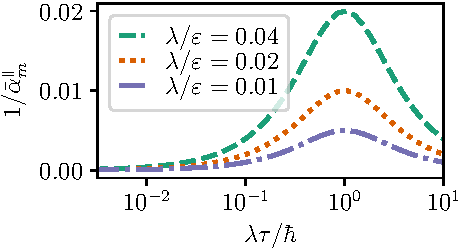
\includegraphics[width=\linewidth]{gfx/alpha_full}
    \caption{Fully vertex-corrected parallel and perpendicular Gilbert damping. In the limit $\lambda\tau\ll1$ we find the limiting behavior $(4)2(\Delta^2+\varepsilon^2)/2$ for $\alpha_{\perp(\parallel)}$. When $\lambda\tau\ll 1$ and $\lambda\tau\gg\Delta/\varepsilon$ we find a scaling behavior $\alpha_{\perp(\parallel)}=(1)2/\lambda^2\tau^2$. Note the use of log-scale on both vertical and horizontal axis. The plot is obtained using $\varepsilon\tau=50$ and $\Delta\tau=0.1$. }
    \label{fig:alpha_plot}
\end{figure}

\begin{figure}
    \centering
    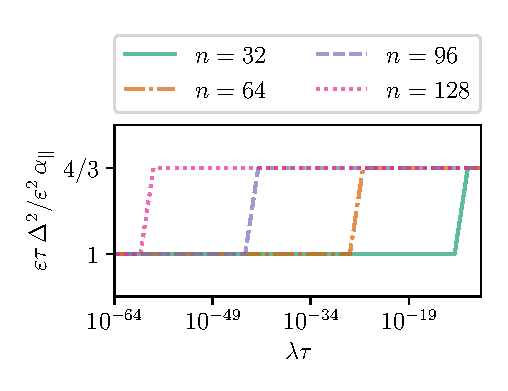
\includegraphics[width=\linewidth]{gfx/numerical_test}
    \caption{The numerical evaluation only yields isotropic Gilbert damping when $\lambda\tau$ is set below numerical precision. The presented plot is independent of chosen values for $\varepsilon\tau$ and $\Delta\tau$ and only depends on the numerical precision $n$, where $n=32,64,96,128$ is the number of digits contained in each variable during computation (a 64 bit double float generally has about 16 digit precision). }
    \label{fig:alpha_plot}
\end{figure}

\section{Introduction}
In the absence of spin-orbit interaction the spin of a conducting electron is conserved. In other words, its spin-life-time is infinite. In a conducting ferromagnet this means that collisions of electrons off of impurities cannot produce a finite spin-polarization and therefore any spin-orbit torque is absent. Furthermore, any rotation of magnetization leaves the electronic spectrum of the conducting electrons unchanged, as such a rotation is identical to a unitary transformation. Gilbert damping then, defined as the response of the spin of conducting electrons to the time-derivative of magnetization, must also be identically zero. Ferromagnets have therefore rather trivial and boring dynamics. In a conducting antiferromagnet however, this is not the case. Here independent rotations of magnetizations on both sublattices do not leave the spectrum invariant, but only a simultaneous rotation of both magnetizations in both sublattices leave the spectrum invariant, which means that the angle between the two magnetization directions must be a conserved quantity. With such a conservation intact, it has the important consequence that the spin on each sublattice is no longer conserved locally and we are allowed to move angular momentum from one sublattice to the other.   

In this Chapter we investigate the role of Rashba spin orbit interaction on the exchange Gilbert damping in a honeycomb antiferromagnet. We find that when the band splitting due to spin orbit is much smaller than the disorder-induced level broadening, disorder averaging will lead to a titanically large value of exchange Gilbert damping, which reflects the fact that it requires many scattering events to randomize the spin of a conducting electron. In the opposite limit where the spin-split bands can indeed be resolved the damping becomes suppressed by many orders of magnitude. Furthermore the damping becomes ultimately anisotropic which was the topic of the previous Chapter. We report that in the antiferromagnetic resonance spectrum we can directly see the effect of the exchange damping. In the large damping regime the magnetic system becomes overdamped and no resonance can be observed. The resonance appears to get a maximum value when the spin-orbit coupling has a value equal to the inverse momentum life-time of conducting electrons. 

Before introducing our model system, let us briefly make a few general observations about conducting antiferromagnets. Consider two magnetization vectors $\bb{m}_\text{A}$ and $\bb{m}_\text{B}$ on two sublattices of a antiferromagnet and furthermore conducting electrons with spin-polarizations $\bb{s}_\text{A(B)}$. An exchange interaction $\Delta$ couples the spin degree of freedom with the magnetization on each sublattice locally, leading to the following equations of motion on magnetization vectors
\beml
\label{basicEQ}
\begin{align}
\dot{\bb{n}}^\textrm{A}  & = \bb{H}^\textrm{A}\times\bb{n}^\textrm{A}  + (J\mathcal{A}/\hbar)\,\bb{n}^\textrm{A}\times \bb{s}^\textrm{A},\\
\dot{\bb{n}}^\textrm{B} & = \bb{H}^\textrm{B}\times\bb{n}^\textrm{B} +(J\mathcal{A}/\hbar)\,\bb{n}^\textrm{B}\times \bb{s}^\textrm{B},
\end{align}
\eml
where $\bb{H}$ is an effective field, $\mathcal{A}$ is the area of the unit cell, and $J$ and $\hbar$ are the (local) exchange energy and reduced Planck's constant ($h/2\pi$) respectively. 

We are interested in the response tensor $\alpha$ relating the spin-polarizations with the time-derivative of magnetizations
\begin{equation}
\label{eq:basicGilbert}
    \begin{pmatrix}
    \bb{s}_\text{A} \\ \bb{s}_\text{B}
    \end{pmatrix}
    =
    \begin{pmatrix}
    \alpha_{11}  &  \alpha_{12} \\ \alpha_{21}  &  \alpha_{22}
    \end{pmatrix}
    \begin{pmatrix}
    \partial_t \bb{m}_\text{A} \\ \partial_t\bb{m}_\text{B}
    \end{pmatrix}.
\end{equation}
The first observation we make is that the presence of sub-lattice-symmetry (the interchanging of the labels $A\leftrightarrow B$) necessarily leads to $\alpha_{11}=\alpha_{22}=\alpha_0$ and $\alpha_{11}=\alpha_{22}=\alpha'$. As written in the introduction when spin-orbit interaction is absent the angle between magnetizations $\bb{m}_\text{A}$ and $\bb{m}_\text{B}$ must be conserved. By inserting Eq.~(\ref{eq:basicGilbert}) into Eq.~(\ref{basicEQ}) we immediately find that $\alpha_0=\alpha'$ so that the damping tensor can be entirely described by the single number $\alpha_0$. Next we introduce the non-staggered and staggered magnetizations 
\begin{equation}
    \bb{m} = \bb{m}_\text{A} + \bb{m}_\text{B}, \quad \bb{n} = \bb{n}_\text{A} - \bb{n}_\text{B},
\end{equation}
and their equations of motion
\begin{align}
    \partial_t{\bb{n}}   & = \bb{H}\times\bb{n}  + \alpha_0 J\mathcal{A}/\hbar\,\bb{n}\times \partial_t\bb{m}\\
    \partial_t{\bb{m}}   & = \bb{H}\times\bb{m}  + \alpha_0 J\mathcal{A}/\hbar\,\bb{m}\times \partial_t\bb{m},
\end{align}
from which one can immediately see that the modulus of both $\bb{m}$ and $\bb{n}$ are conserved. Alternatively one can reach the same conclusion by noting that $\partial_t (\bb{m}_\text{A}\cdot\bb{m}_\text{B}) = \partial_t (m^2-n^2) = 0$ and that by construction $n^2+m^2=1$, from which it immediately follows that $\bb{m}\cdot\partial_t\bb{m} = \bb{n}\cdot\partial_t\bb{n} = 0$. 


\section{Role of vertex-corrections on the asymptotic behavior of $\alpha_{m,zz}$ and $\alpha_{m,\parallel}$}
It was shown in the previous Chapter that in the limit $\lambda\tau\ll1$ the damping tensor becomes isotropic, while in the opposing limit we find an ultimate anisotropy where $\alpha_{m,zz}$ vanishes completely. In the latter limit, the spin-split bands are completely resolved and certain spin-flip processes become forbidden. A more quantitative discussion on how $\alpha_{m,zz}$ and $\alpha_{m,\parallel}$ however, will be presented here. 

It is instructive to illustrate the role of disorder averaging in both limits as it turns out, the role of vertex-corrections on the components of the $\alpha_m$ tensor has a profound effect when $\lambda\tau/\hbar\ll1$, but negligible when $\lambda\tau/\hbar\gg1$. 

In the limit $\Delta_\text{sd}$ we are able to obtain concise and exact analytical formulas, that we present first. In this limit the exchange damping tensor can be fully characterized by just two numbers, $\alpha_m=\diag\left(\alpha_{m,\parallel}, \alpha_{m,\parallel}, \alpha_{m,zz}\right)$.

We will annotate the tensor-components with a superscript $(i)$, that denotes the number of disorder-lines inserted into the diagram. Physically, it means averaging over various disorder ensembles where the electron scatters $i$ number of times. 

Let us first consider the ``bare bubble'' contribution which describes an electron entering and exiting the system without a single scattering event
\begin{align}
    \alpha_{m,zz}^{(0)} =  & \frac{\varepsilon\tau}{\hbar} \frac{1-(\lambda/2\varepsilon)^2}{1+(\lambda\tau)^2},\\
    \alpha_{m,\parallel}^{(0)} =  & \frac{\varepsilon\tau}{\hbar}\left(\frac{1}{2}\frac{3+2(\lambda\tau/\hbar)^2}{1+(\lambda\tau/\hbar)^2}-\frac{2}{(4-\lambda/\varepsilon)^2}\right),
\end{align}
where one can immediately see the asymptotic behavior for large and small values of $\lambda\tau$:
\begin{align}
    \alpha_{m,zz}^{(0)}  & = \frac{\epsilon\tau}{\hbar}\begin{cases}
    1  +\mathcal{O}(\lambda/\varepsilon)  & \text{ for }\lambda\tau/\hbar\ll1\\
    \hbar/(\lambda\tau)^2 & \text{ for }\lambda\tau/\hbar\gg1
    \end{cases},\\
    \alpha_{m,\parallel}^{(0)}  & = \frac{\epsilon\tau}{\hbar}\begin{cases}
    1  +\mathcal{O}(\lambda/\varepsilon)  & \text{ for }\lambda\tau/\hbar\ll1\\
    1/2 + \hbar/2(\lambda\tau)^2 & \text{ for }\lambda\tau/\hbar\gg1.
    \end{cases}
\end{align}
Evidently, the exchange damping transitions from fully isotropic to ultimately anisotropic when changing the limits $\lambda\tau\ll1$ to $\lambda\tau\gg1$. 
Including a small number of scattering events in the calculation we find an interesting modification:
\begin{align}
    \alpha_{m,zz}^{(i)}  & = \frac{\epsilon\tau}{\hbar}\begin{cases}
    i + \mathcal{O}(\lambda/\varepsilon)  & \text{ for }\lambda\tau/\hbar\ll1\\
    \hbar/(\lambda\tau)^2 & \text{ for }\lambda\tau/\hbar\gg1,
    \end{cases}\\
    \alpha_{m,\parallel}^{(i)}  &  = \frac{\epsilon\tau}{\hbar}\begin{cases}
    i + \mathcal{O}(\lambda/\varepsilon)  & \text{ for }\lambda\tau/\hbar\ll1\\
    1-(1/2)^{i+1}+\mathcal{O}(\hbar/(\lambda\tau)^2) & \text{ for }\lambda\tau/\hbar\gg1.
    \end{cases}
\end{align}
In the large $\lambda\tau$ limit the $zz$ component of the $\alpha_m$ tensor is unchanged by scattering events, whereas the parallel component quickly converges to the value of $\varepsilon\tau$. In the opposite limit, where the components remain isotropic with respect to each other, the components have a profound sensitivity to scattering events. Each scattering event contributes a value of $1\,\varepsilon\tau$ to the damping coefficient. While at a first glance it appears as strong sensitivity to impurities, it in reality reflects a long spin-life time: many scattering events are required to randomize the spin of an electron. 

In a truly diffusive system one should take the limit $i\rightarrow\infty$, in which case the tensor components are given by
\begin{align}
\label{eq:alphaparallelzerodelta}
    \alpha_{m,zz}^{(\infty)}  & = \frac{\epsilon \tau}{\hbar}\, \frac{2}{(2-n_z^2)\lambda^2\tau^2},\\
    \alpha_{m,\parallel}^{(\infty)}  & = \frac{\varepsilon\tau}{\hbar}\,\frac{2\,(1+\lambda^2\tau^2)}{(2-n_z^2)\lambda^2\tau^2}.
\end{align}

We plot the functions of $\alpha_{m,zz(\parallel)}^{(i)}$ for $i=0,1,2$ and $i\rightarrow\infty$ in Fig.~\ref{fig:alpha_plot}. 
\begin{figure}
    \centering
    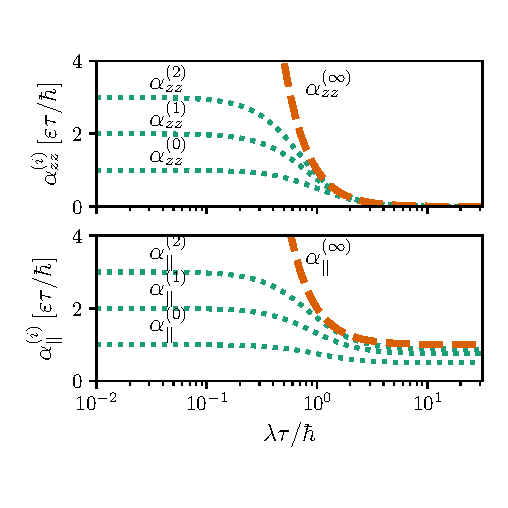
\includegraphics[width=\linewidth]{gfx/Chapter04/alpha_plot2}
    \caption{The first three scattering contributions $\alpha_{m,zz}^{(i)}$, $i=0,1,2$ (green, dotted) and the fully vertex corrected $\alpha_{m,zz}^{(\infty)}$ (orange, dashed) as a function of $\lambda \tau$. }
    \label{fig:alpha_plot}
\end{figure}
We find that indeed in the limit $\lambda\tau\gg1$ becomes ultimately anisotropic where $\alpha_{m,zz}$ becomes vanishingly small. Moreover, we find a substantial drop of $\alpha_{m,\parallel}$ for increasing values of $\lambda\tau$, that can reach a difference of many orders of magnitude. 

We note that a large value for damping corresponds to an overdamped regime, which we will explain in details in the next section. The direct exchange parameter $\Delta$ can be included perturbatively in both overdamped and underdamped regimes. In the overdamped regime,  $\Delta$ merely introduces a cutoff whereas in the underdamped regime a small modification.
\begin{align}
\label{eq:alphaparallelzerodelta}
    \alpha_{m,zz}^{(\infty)}  & = \frac{\epsilon \tau}{\hbar}\, \frac{2}{(2-n_z^2)\lambda^2\tau^2+2\Delta^2/\varepsilon^2},\\
    \alpha_{m,\parallel}^{(\infty)}  & = \frac{\varepsilon\tau}{\hbar}\,\frac{2(1+\lambda^2\tau^2)}{(2-n_z^2)\lambda^2\tau^2+2\Delta^2/\varepsilon^2}.
\end{align}
{\color{blue} Need to find correct coefficients for the underdamped regime ($\lambda\tau\gg1$)}
that we illustrate in Fig.~\ref{fig:alpha3}.
\begin{figure}
    \centering
    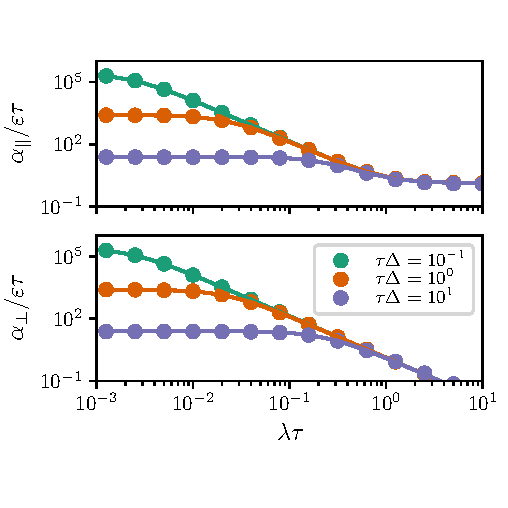
\includegraphics{gfx/Chapter04/alpha_plot1.pdf}
    \caption{Fully dressed damping components $\alpha_{\parallel,\perp}$ as a function of $\lambda\tau$ for three values of $\Delta\tau$. Note the use of log-scale on both horizontal and vertical axes.}
    \label{fig:alpha3}
\end{figure}
{\color{blue} (Need to check/update the coefficients and limits. }
%
% uniform modes
%
\section{Uniform modes in collinear ground state}
When subjecting an AFM to an oscillating magnetic field, the localized spins will exhibit a precession parallel to the magnetic field direction. By tuning the magnetic field's frequency to an internal harmonic frequency we can observe resonance. As shown first by Kittel and Keffer \cite{PhysRev.82.565, PhysRev.85.329} the resonance frequency is proportional to the square root of the product of anisotropy and exchange energy. The width of the resonance frequency however, as we show below, is linearly proportional to anisotropy and exchange damping. Although exchange damping remains finite, even large, at vanishingly small values of spin-orbit interaction, the anisotropy must vanish. A direct calculation from the grand potential (see Appendix~\ref{app:D}), we find that the Rashba honeycomb lattice exhibits an out-of-plane and easy-axis anisotropy. Close to $\bb{n}=\bb{n}_\perp$ the magnetostatic anisotropy energy is given by
\begin{equation}
    E = -\frac{K}{2}n_z^2, \quad K= \frac{1}{2\pi\hbar^2v^2}\begin{cases}
    |\Delta^2\lambda|  &  \text{for } |\lambda/2\Delta| \geq 1 \\
    |\Delta\lambda^2|  &  \text{for } |\lambda/2\Delta| \leq 1
    \end{cases}.
\end{equation}

The transition from $|\lambda/2\Delta|\le1$ to $|\lambda/2\Delta|\ge1$ correspond to the merger of two of the bands as illustrated in Fig.~\ref{fig:bands}. The resonance frequencies and widths are obtained by including the effect of anisotropy in the equations of motion on $\bb{n}$ and $\bb{m}$
\beml
\label{AFMEOM2}
\begin{align}
\label{ndot2}
\dot{\bb{n}} = &  -\Omega\, \bb{n}\!\times\!\bb{m} +K \bb{m}\!\times\!\bb{n}_\perp+\bar{\alpha}_m\,\bb{n}\!\times\!\dot{\bb{m}}+\alpha_n\,\bb{m}\!\times\! \dot{\bb{n}},\\
\label{mdot2}
\dot{\bb{m}} = & K  \bb{n}\!\times\!\bb{n}_\perp+\alpha_n\,\bb{n} \times \dot{\bb{n}}+\bar{\alpha}_m \bb{m} \times \dot{\bb{m}} ,
\end{align}
\eml
To obtain the resonance frequency and width we follow a standard recipe of linearization \cite{kittel}. First expand the (non)-staggered magnetizations around the classical ground-state solution
\begin{align}
    \bb{n}\rightarrow\hat{\bb{z}} + \delta\bb{n}_\parallel,\quad \bb{m}\rightarrow \delta\bb{m}_\para,
\end{align} 
(where $\delta m_\perp$ is omitted to ensure that $\bb{n}\cdot\bb{m}=1+\mathcal{O}(\delta^2)$) and keep only first order contributions in the equations of motion of Eqs.~(\ref{AFMEOM2}). The harmonics $\omega$ are obtained by replacing $\partial_t \rightarrow i\omega$ through which we arrive at a linear system of equations. We find the real and imaginary parts of $\omega = \omega_0 + i \delta\omega$ to be
\begin{align}
    \omega_0 = \sqrt{K(\Omega + K(1- \alpha_m^2 / 4))},\quad \delta\omega =  \frac{K \alpha_m + \Omega \alpha_n }{2(1- \alpha_n \alpha_m)},
\end{align}
{\color{blue} or further to:
\begin{align}
    \omega_0 = \sqrt{K\Omega},\quad \delta\omega =  \frac{K \alpha_m}{2},
\end{align}
}
where we used that $\alpha_n\ll\alpha_m$.
% \be
% \omega = \frac{\sqrt{2 K(K+ \Omega)(1+ \alpha_m^\parallel \alpha_n - \alpha_n^2) + 4 K^2 - K^2 (\alpha_m^{\parallel})^2}}{2 +2 \alpha_n^2 - 2 \alpha_n \alpha_m^\parallel}
% \e
% Using that $\alpha_n\ll\alpha_m$,  we arrive at the more compact expression
% \be
% \re \omega = \sqrt{K(\Omega + K - K \alpha_m^2 / 4)}
% \e
% the width of the resonance line will be given by the imaginary part of the $\omega$:
% \be
% \delta\omega \equiv \im \omega = \frac{K (\alpha_m - 2 \alpha_n) + \Omega \alpha_n }{2 +2 \alpha_n^2 - 2 \alpha_n \alpha_m}.
% \e
The ratio $\delta\omega/\omega_0$ {\color{blue} does this have a name?} can be minimized with respect to $\lambda$ when $\lambda\tau\sim1$. In the limit $\Delta/\varepsilon\rightarrow0$ it can be seen from Eq.~(\ref{eq:alphaparallelzerodelta}) that the minimum is achieved at exactly $\lambda\tau=1$. For small values of $\Delta/\varepsilon$ the minimum is slightly shifted according to:
\begin{equation}
    \lambda\tau = 1 + \frac{8\Delta^2/\varepsilon^2}{2-n_z^2}+\mathcal{O}\Big(\frac{\Delta^4}{\varepsilon^4}\Big).
\end{equation}
In this limit we find after dropping $\alpha_n$ and neglecting terms $\mathcal{O}(K/\Omega)$ we get the result

% The in-plane damping that appears in the resonance frequency width can be minimized with respect to $\tau$ when $\lambda\tau/\hbar = 1$, which corresponds to \begin{equation}\alpha_{m,||}^{(\infty)}=\frac{\varepsilon}{\lambda}\frac{3-(\lambda/\varepsilon)^2}{1-(\lambda/2\varepsilon)^2}, \end{equation}
% the normalized resonance width  $\delta\omega/\omega$ is then given by
\begin{align}
    \frac{\delta\omega}{\omega}  & \simeq \frac{\sqrt{K}\alpha_m}{2\sqrt{\Omega}}\nonumber\\
     & \simeq\frac{1}{2\sqrt{2\pi}\hbar v}\frac{3\varepsilon}{\sqrt{\Omega}} \begin{cases}
    |\Delta/\sqrt{\lambda}|  &  \text{for } |\lambda/2\Delta| \geq 1 \\
    \sqrt{|\Delta|}  &  \text{for } |\lambda/2\Delta| \leq 1.
    \end{cases}
    \label{eq:freq}
\end{align}
We consider the regimes (1) The limit $\lambda\tau\ll1$ and $\Delta\ll\lambda$, (2) the limit $\lambda\tau\ll1$ and $\Delta\gg\lambda$, (3) $\lambda\tau=1$ and (4) $\lambda\tau\gg1$. For each regime we find:
\begin{align}
    (1) & \quad \frac{\delta\omega}{\omega}= \frac{1}{2\sqrt{2\pi} v}\frac{1}{\sqrt{\Omega}}\frac{\varepsilon\Delta}{\lambda^{3/2}\tau}\\
    (2) & \quad \frac{\delta\omega}{\omega}= \frac{1}{2\sqrt{2\pi} v\hbar^2}\frac{1}{\sqrt{\Omega}}\frac{\varepsilon^3\lambda\tau}{\Delta^{3/2}}\\
    (3) & \quad \frac{\delta\omega}{\omega}= \frac{1}{2\sqrt{2\pi}\hbar v}\frac{3\varepsilon}{\sqrt{\Omega}} \begin{cases}
    |\Delta/\sqrt{\lambda}|  &  \text{for } |\lambda/2\Delta| \geq 1 \\
    \sqrt{|\Delta|}  &  \text{for } |\lambda/2\Delta| \leq 1.
    \end{cases}\\
    (4) & \quad \frac{\delta\omega}{\omega}= \frac{\varepsilon\tau}{2\sqrt{2\pi} v\hbar^2}\frac{1}{\sqrt{\Omega}}
    \begin{cases}
    |\Delta\sqrt{\lambda}|  &  \text{for } |\lambda/2\Delta| \geq 1 \\
    |\sqrt{\Delta}\lambda|  &  \text{for } |\lambda/2\Delta| \leq 1.
    \end{cases} 
\end{align}
{\color{blue} Still have to edit above equations}

The ratio $\delta\omega/\omega$ is plotted for few values of $\Delta$ in Fig.~\ref{fig:freqs}
\begin{figure}
    \centering
    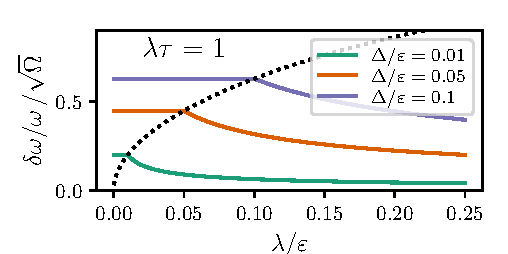
\includegraphics{gfx/Chapter04/freq_plot.pdf}
    \caption{Frequency for the optimal case $\lambda\tau=1$ for few values of $\Delta$. The black dotted curve corresponds to Eq.~(\ref{eq:freq}) for $\lambda=\Delta$}. 
    \label{fig:freqs}
\end{figure} % Highly anisotropic Gilbert Damping
\cleardoublepage
\addtocontents{toc}{\protect\vspace{\beforebibskip}}%


%%%%%%%%%%%%%%%%%%%%%%%%
\chapter{Conclusions}
%%%%%%%%%%%%%%%%%%%%%%%%
In the introduction of this thesis we set the goal of this thesis: to investigate the role of conducting electrons in Dirac ferro- and antiferromagnets on the manipulation and relaxation of magnetic moments. The study was motivated in part by an abundance of phenomological models, but a relatively small amount of microscopic models. We proposed to model the manipulation and relaxation of magnetic moments using the $s$--$d$ model. Here the spins of conducting electrons interact on a local level with localized spins. The relaxation mechanism is provided by a random scalar potential. By scattering off impurities, conducting electrons can transfer their angular momentum to the lattice. The dissipation of magnetic moments is then mediated by electron-impurity scattering in the presence of spin-orbit interaction. 

In Chapter~\ref{ch:sdmodel} we derived the classical equations of motion of the localized spins and showed that they are coupled to the spin-density of the conducting electrons. The spin-densities can be computed using linear response theory and are typically computed in response to electric currents and in responses to time-derivatives of magnetizations. The former defines spin-orbit torques that are induced by electric currents, while the latter defines Gilbert damping that describes the relaxation of magnetizations. In Chapters~\ref{ch:diffusive}\&\ref{ch:baglay} we used this methodology to obtain analytical solutions for spin-orbit torques and Gilbert dampings. On the other hand, in Chapters~\ref{ch:summit} a numerical approach based on scattering wave functions was used to obtain current induced spin-orbit torques in a honeycomb N\'eel antiferromagnet. 


In Chapter~\ref{ch:diffusive} we considered a bilayer system consisting of a topological insulator (e.g. Bi$_2$Se$_3$ or Bi$_2$Te$_3$) and a ferromagnetic insulator (e.g. YIG or EuO) and computed the spin-densities in linear response at finite frequency $\omega$ and momentum $\bb{q}$. A diffusive response is found in the direction perpendicular to the topological insulator surface. Such a response leads to strong non-adiabatic anti-damping spin-orbit torque that identify as a novel diffusive anti-damping spin-orbit torque. Note that in non-topological ferromagnetic systems strong diffusive responses exist as well, but are always directed in the direction of magnetization and therefore do not produce a finite torque due to the vector product involved (i.e. $\bb{m}\times\bb{m}=\bb{0}$). The spin-momentum locking in topological insulators leads to a self-energy of the form $\Sigma = i\pi\alpha(\varepsilon-\Delta_\text{sd} m_z)$ that is responsible to the perpendicular-to-the-plane diffusive response. As mentioned in Chapter~\ref{ch:sdmodel} 

Analytical solutions are easily obtained for rather "symmetric" systems. The Fermi-surface are isotropic with respect to momentum leading to easy integration. Including finite magnetizations in antiferromagnets in general give rise to anisotropic Fermi-surfaces and can only be treated perturbatively. 

To overcome these difficulties, we developed a numerical method in Chapter~\ref{ch:summit} that can be used to obtain spin-orbit torques for any system. As mentioned in Chapter~\ref{cd:sdmodel}, damping-like torques must be even in transport time and are generally absent in microscopic studies. We found that anisotropic Fermi surface do lead to even-in-transport-time contributions to the spin-torques and thus finite damping-like torques. This asserts that the numerical method is powerful and useful in further research in current induced dynamics. We note that this method unfortunately does not provide any insight in Gilbert dampings. The python package kwant that we used, does provide however a new functionality called the Kernel Polynomial Method (KPM). Using KPM we can expand exact Green's functions in Chebychev polynomials, that can be used to efficiently compute any two-point correlator. In other words it can be used to compute spin-densities in reponse to electric current and time-derivatives of magnetizations. This method is currently implemented to verify the results from Chapters~\ref{ch:summit}\&\ref{ch:baglay} and will be used to explain recent findings of anisotropic spin-orbit torques and dampings in zig-zag antiferromagnets and other systems.



%%%
In conclusion, we consider magnetization dynamics in a model TI/FM system at a finite frequency $\omega$ and $\bb{q}$ vector. We identify novel diffusive anti-damping spin-orbit torque that is specific to TI/FM system.  Such a torque is absent in usual (non-topological) FM/metal systems, where the diffusive response of conduction electron spin density is always aligned with the magnetization direction of the FM. In contrast, the electrons at the TI surface gives rise to singular diffusive response of the conduction electron spin-density in the direction perpendicular to the TI surface, irrespective of the FM magnetization direction. Such a response leads to strong non-adiabatic anti-damping spin-orbit torque that has a diffusive nature. This response is specific for a system with an ultimate spin-momentum locking and gives rise to abnormal anti-damping diffusive torque that can be detected by performing spin-torque resonance measurements. We also show that, in realistic conditions, the anti-damping like diffusive torque may become orders of magnitude larger than the usual field like spin-orbit torque. We investigate the peculiar magnetizations dynamics induced by the diffusive torque at the frequency of the ferromagnet resonance. Our theory also predicts ultimate anisotropy of the Gilbert damping in the TI/FM system. In contrast, to the phenomenological approaches \cite{vanderBijl2012,Hals2013} our microscopic theory is formulated in terms of very few effective parameters. Our results are complementary to previous phenomenological studies of Dirac ferromagnets \cite{tserkovnyak_theory_2009,mahfouzi_spin-orbit_2012,katsnelson15,fischer_spin-torque_2016,yokoyama_theoretical_2010,yokoyama_current-induced_2011,siu_spin_2016,mahfouzi_antidamping_2016,soleimani_spin-orbit_2017,kurebayashi_microscopic_2017,chen_current-induced_2017,rodriguez-vega_giant_2016,qi_topological_2008,garate_inverse_2010,yokoyama_theoretical_2010,yokoyama_current-induced_2011,nomura_electric_2010,tserkovnyak_thin-film_2012-1,linder_improved_2014,tserkovnyak_spin_2015,ueda_topological_2012,liu_reading_2013,chang_nonequilibrium_2015,fischer_spin-torque_2016,mahfouzi_antidamping_2016,fujimoto_transport_2014,okuma_unconventional_2016}.

Motivated by recent experiments on the N\'eel vector switching we investigate microscopically the spin-orbit torques in an $s$--$d$-like model of a two-dimensional honeycomb antiferromagnet with Rashba spin-orbit coupling. We investigated the model with preserved and broken sublattice symmetry and distinguished metal and half-metal regimes for each of the model. Spin-orbit interaction in combination with on-site disorder potential and local exchange coupling between conduction and localized spins have been responsible for a microscopic mechanism of the angular momentum relaxation. We find identically vanishing anti-damping and N\'eel spin-orbit torques in the symmetric model in all regimes considered. As the result, the metal regime of the symmetric model is characterized by a particularly simple isotropic field-like spin-orbit torque, while the half-metal regime is characterized by anisotropic spin-orbit torques of the field-like symmetry.  Finite and anisotropic anti-damping torques, that crucially depend on disorder strength, are found in both metal and half-metal regimes of the asymmetric model. We also find non-equilibrium staggered polarization in the half-metal regime of the asymmetric model. This formally leads to a finite value of the N\'eel spin-orbit torque, which is, however, not a quantity of interest in that model. Overall, our results reveal the importance of two-dimensional electron momentum confinement for spin-orbit torque anisotropy. Largest values of spin-orbit torques are also associated with the half-metal regimes of conduction in both models. 

In this Chapter, we demonstrate that the presence of sufficiently strong spin-orbit coupling $\lambda\tau/\hslash \gg 1$ results in the ultimate anisotropy of the Gilbert damping tensor in the metal regime, $\ep_F\gg\Delta_{\text{sd}}+\lambda$.  One can trace the phenomenon to the spin-orbit induced splitting of Fermi surfaces that forbids scattering processes that are responsible for the relaxation of certain magnetization and N\'eel vector components. 

We also demonstrate that a finite in-plane projection $\bb{n}_\parallel$ of the N\'eel vector is responsible for a weak anisotropy of conductivity and spin-orbit torques for Fermi energies approaching the band edge, $\ep_F \sim \Delta_{\text{sd}}+\lambda$. This anisotropy is, however, absent in the metallic regime. 

Gilbert damping is, however, isotropic in the absence of spin-orbit interaction as it is required by symmetry considerations. Thus, we demonstrate that the onset of Rashba spin-orbit interaction in 2D or layered AFM systems leads to a giant anisotropy of Gilbert damping in the metallic regime. The physics of this phenomenon originates in spin-orbit induced splitting of the electron subbands that destroys a particular decay channel for magnetization and leads to undamped precession of the N\'eel vector. The phenomenon is based on the assumption that other Gilbert damping channels  (e.\,g. due to phonons) remain suppressed in the long magnon wavelength limit that we consider. The predicted giant Gilbert damping anisotropy may have a profound impact on the N\'eel vector dynamics in a variety of 2D and layered AFM materials. 

%%%%
% ********************************************************************
% Backmatter
%*******************************************************
\appendix
\renewcommand{\thechapter}{\alph{chapter}}
\cleardoublepage
\part{Appendix}
%************************************************
\chapter{Linear Response}\label{ch:linearesponse}
%************************************************
\section{Linear Response Theory}
The main results derived in this thesis are obtain from linear response theory. Let us briefly consider a Hamiltonian $H$ subject to a small perturbation $\delta H$. We are interested in the effect of $\delta H$ on an observable $O$. To linear order in $\delta H$ this is captured by the Kubo formula:
\begin{equation}
	\bar{O} = \frac{i}{h} \int \mathrm{d}\varepsilon\, f(\varepsilon-\mu) \tr\big(G^\text{R}...\big),
	\label{eq:kubo1}
\end{equation}
where $G^\text{R(A)}_{\bb{p}',\omega'}$ are the retarded(advanced) Green functions with momentum $\bb{p}'$ and frequency $\omega'$. This linear response formula is evaluated in momentum and frequency space, however in some cases it is more convenient to work in the position and time space and we will use the Kubo-Greenwood formula:
\begin{equation}
	...
\end{equation}
In transport theory a common example of linear response is the calculation of the conductivity tensor, whose components are calculated as the a velocity-velocity response. It is interesting to note that one can obtain conductivity from current-current correlation. This is a consequence of the fluctuation-dissipation theorem. 

Before discussing details on how we treat disorder-potentials, let us first derive Eq.~\ref{eq:kubo1}. 
The $dc$ linear-response formulas that we use are given by:
\begin{align}
    \bb{s}^\pm_\alpha = \int\frac{\mathrm{d}^2\bb{p}}{(2\pi)^2}\,\tr \langle G_{\bb{p}}^\text{R} \hat{{\chi}}_\alpha G_{\bb{p}}^\text{A} \hat{s}_\beta\rangle ,
\end{align}
where $G_{\bb{p}}^\text{R(A)}$ are retarded and advanced Green function in momentum-space, $\hat{s}^+ = \sigma_\beta$, $\hat{s}_\beta^-=\sigma_\beta\Sigma_z \Lambda_z$ are the operators corresponding to the spin-polarization $\bb{s}^+$ and staggered spin-polarization $\bb{s}^-$, $\hat{\chi}_\alpha$ is the perturbation that the spin-density is in response to, and the angular brackets $\langle\cdots\rangle$ denote disorder-averaging which will be explained below. The response to electric current density $\bb{j}$ is defined by $\hat{\chi}_\beta = (e v /\sigma_{xx})\, \Sigma_\beta$, where $\sigma_{xx}$ is the longitudinal conductivity (measured in units of e$^2$/h) as defined in Eq.~(\ref{intro:eq:long_cond}). Response to magnetization $\partial_t m_\beta$ and $\partial_t n_\beta$, is defined through $\hat{\chi}_\beta = \Delta \sigma_\beta$ and $\hat{\chi}_\beta = \Delta \sigma_\beta \Sigma_z\Lambda_z$. 

Our formula for linear-response is defined for zero temperature and we neglect contributions originating from the Fermi-sea (the so-called Streda contribution).  In most samples it is inevitable to have a certain degree of disorder. It is therefore important to take into account disorder in our calculations. As mentioned in the Main Text, we model disorder as an average ensemble of impurities with short-range on-site potential. In order to quantify the effect of disorder, two important steps must be performed. Firstly, we replace the clean Green functions in the linear response formula, with disordered ones. Secondly we replace one of the vertices with one that is corrected with disorder-averaging.

In order to replace the bare Green function with a disordered one, one needs to include a self-energy. This self-energy gives rise to the finite momentum-life-time of the electron and restores translational invariance.  In low concentration of impurities (which we refer to as the clean metal limit, i.e. $\alpha\rightarrow0$) and neglecting contributions from rare-scattering events (such as multiple scattering off the same impurity), one can use the Born approximation

\begin{equation}
\Sigma^\text{R(A)} = 2\pi\alpha \int \frac{\mathrm{d}\bb{p}}{(2\pi)^2}\,G^\text{R(A)}_{\vec{p},\varepsilon},
\end{equation}

whose imaginary part is given by $\im \Sigma^\text{R(A)} = \pi\alpha/4\,(\varepsilon + \Delta \bb{l}\cdot\bb{\sigma}\Sigma_z\Lambda_z)$. The real-part of the self-energy leads to a small spectrum-shift that we do not consider. 

For the second step in disorder averaging, we need to replace one of the vertex functions with one that is corrected for disorder in the ladder approximation (as illustrated in Figure~\ref{fig:diagrams}-b). We call this new vertex function the vertex-corrected function. 
By denoting $\hat{\chi}^{\text{vc}}$ as the vertex-corrected function of $\hat{\chi}$ and $\hat{\chi}^i$ as the function containing $i$ disorder-lines, the ladder approximation is given by:
\begin{align}
    \hat{\chi}^\text{vc}
      &=           
        \hat{\chi}+\hat{\chi}^1+\hat{\chi}^2+\cdots,
        \label{intro:eq:ladder}
\end{align}
where $\hat{\chi}^i$ is given by:
\begin{align}
    \hat{\chi}^\text{i} = 2\pi\alpha_d\int\frac{\mathrm{d}^2\bb{p}}{(2\pi)^2} G_{\bb{p}}^\text{R}\hat{\chi}^\text{i-1}G_{\bb{p}}^\text{A}
    \label{intro:eq:onedisorderline}
\end{align}

%********************************************************************
% Appendix
%*******************************************************
% If problems with the headers: get headings in appendix etc. right
%\markboth{\spacedlowsmallcaps{Appendix}}{\spacedlowsmallcaps{Appendix}}
\chapter{Calculation Details to Chapter 2}
\section{Kubo formula}
The linear response formula used in the main text can be obtained in a Keldysh-framework. We start by introducing the Green function $\mathcal{G}$ in rotated Keldysh space [see e.g. Ref.~\cite{rammer_quantum_1986}]
\begin{equation}
    \mathcal{G}=\begin{pmatrix}G^\text{R}&G^\text{K}\\0&G^\text{A}\end{pmatrix}
\end{equation}
where R, A and K denote retarded, advanced and Keldysh Green functions respectively. In this notation a perturbation to a classical field $V(\bb{x},t)$ is given by
\begin{multline}
    \delta\mathcal{G}(\bb{x}_1,t_1;\bb{x}_2,t_2)=\int\!d\bb{x}_3\int\!dt_3\, \mathcal{G}^{(0)}(\bb{x}_1,t_1;\bb{x}_3,t_3)\\\hat{V}(\bb{x}_3,t_3)\mathcal{G}^{(0)}(\bb{x}_3,t_3;\bb{x}_2,t_2)+\mathcal{O}(V^2)
    \label{chap1:eq:s2}
\end{multline}
with $\mathcal{G}^{(0)}$ equilibrium Green functions. The Wigner-transform of a function $F(\bb{x}_1,t_1;\bb{x}_2,t_2)$ is given by
  \begin{multline}
    F(\bb{x}_1,t_1;\bb{x}_2,t_2)=\int\frac{d^2\bb{p}}{(2\pi\hslash)^2}\int \frac{d\ep}{2\pi\hslash}\,e^{-i\ep(t_1-t_2)/\hslash}e^{i\bb{p}\cdot(\bb{x}_1-\bb{x}_2)/\hslash}F(\ep,\bb{p},R,T)
   \end{multline}
with energy $\ep$, momentum $\bb{p}$, time $T=\frac{t_1+t_2}{2}$ and position $\bb{R}=\frac{\bb{x}_1+\bb{x}_2}{2}$. In equilibrium the Green functions $\mathcal{G}^{(0)}$ do not depend on $\bb{R}$ and $T$, so that the momentum-frequency representation of Eq.~(\ref{chap1:eq:s2}) becomes 
   $\delta\mathcal{G}(\ep,\omega,\bb{p},\bb{q})= \mathcal{G}^{(0)}_{\ep_+,\bb{p}_+} V_{\omega,\bb{q}}\mathcal{G}^{{(0)}}_{\ep_-,\bb{q}_-}$, 
with subscripts $\ep_\pm=\ep\pm\hslash\omega/2$ and $\bb{p}_\pm=\bb{p}\pm\hslash\bb{q}/2$ and $V_{\omega,\bb{q}}$ the Fourier transform of $V(\bb{R},T)$. 

The spin density $\bb{s}_{\omega,\bb{q}}$ is given by
\begin{equation}
    \bb{s}_{\omega,\bb{q}} = {i\hslash} \int\!\frac{d\ep}{2\pi\hslash}\int\!\frac{d^2\bb{p}}{(2\pi\hslash)^2}\tr \left[\delta G^<({\ep,\omega,\bb{p},\bb{q}},T) \bb{\sigma}\right],
\end{equation}
where,
\begin{multline}
    \delta G^<(\ep,\omega,\bb{p},\bb{q}) = 1/2 \big(\delta G^\text{K}(\ep,\omega,\bb{p},\bb{q})-
    \delta G^\text{R}(\ep,\omega,\bb{p},\bb{q})+\delta G^\text{A}(\ep,\omega,\bb{p},\bb{q})\big).  
\end{multline}
In equilibrium we have the fluctuation-dissipation theorem $   G^\text{K}_{\ep_\pm,\bb{p}_\pm} = (1-2f_{\ep_\pm})(G^\text{R}_{\ep_\pm,\bb{p}_\pm}-G^\text{A}_{\ep_\pm,\bb{p}_\pm}) $ with $f_{\ep_\pm}$ the Fermi distribution, so that the spin density now becomes
\begin{align}
    \bb{s}_{\omega,\bb{q}} =& {i\hslash} \int\!\frac{d\ep}{2\pi\hslash}\int\!\frac{d^2\bb{p}}{(2\pi\hslash)^2}\tr\langle
     -(f_{\ep_+}-f_{\ep_-})\bb{\sigma}G^\text{R}_{\ep_+,\bb{p}_+} V_{\omega,\bb{q}}G^\text{A}_{\ep_-,\bb{p}_-}\nonumber\\
    &\hspace{3cm}-f_{\ep_+}\bb{\sigma}G^\text{R}_{\ep_+,\bb{p}_+} V_{\omega,\bb{q}}G^\text{R}_{\ep_-,\bb{p}_-}
    +f_{\ep_-}\bb{\sigma}G^\text{A}_{\ep_+,\bb{p}_+} V_{\omega,\bb{q}}G^\text{A}_{\ep_-,\bb{p}_-}\rangle,
\end{align}
where the angular brackets stands for impurity averaging. The latter amounts to the replacement of the Green's functions with the corresponding impurity averaged Greens functions (in Born approximation) and to the replacement of one of the spin operators with the corresponding vertex corrected operator (in the non-crossing approximation). The corrections beyond the non-crossing approximation are important for those tensor components that lack leading-order contribution \cite{ivan}. To keep our notations more compact we ignore here the fact that the Green's functions before disorder averaging lack translational invariance, i.\,e. depend on both Wigner coordinates: momentum and coordinate. 

In the limit of small frequency, i.e. $\hslash\omega\ll\ep$, we obtain $s_\alpha = s^\text{I}_\alpha+s^\text{II}_\alpha$,
\begin{align}
    s^\text{I}_\alpha&=\frac{i\omega}{2\hslash}\int\frac{d\ep}{2\pi}\int \frac{d^2\bb{p}}{(2\pi)^2}\Big(-\frac{\partial f}{\partial \ep}\Big)\tr\big\langle
    2\sigma_\alpha G^\text{R}_{\ep_+,\bb{p}_+} V_{\omega,\bb{q}} G^\text{A}_{\ep_-,\bb{p}_-}
    \nonumber\\
    &\hspace{3cm}-\sigma_\alpha G^\text{A}_{\ep_+,\bb{p}_+} V_{\omega,\bb{q}} G^\text{A}_{\ep_-,\bb{p}_-} -\sigma_\alpha G^\text{R}_{\ep_+,\bb{p}_+} V_{\omega,\bb{q}} G^\text{R}_{\ep_-,\bb{p}_-}\big\rangle,\\
    s^\text{II}_\alpha&=\frac{i}{\hslash}\int\frac{d\ep}{2\pi}\int \frac{d^2\bb{p}}{(2\pi)^2} f_\ep \tr \big\langle\sigma_\alpha
    G^\text{A}_{\ep_+,\bb{p}_+} V_{\omega,\bb{q}} G^\text{A}_{\ep_-,\bb{p}_-}-
    \sigma_\alpha G^\text{R}_{\ep_+,\bb{p}_+} V_{\omega,\bb{q}} G^\text{R}_{\ep_-,\bb{p}_-}\big\rangle,
\end{align}
where $s^{\text{I}}$ and $s^\text{II}$ are the Kubo and Streda contributions respectively. The Streda contribution is sub-leading in the powers of weak disorder strength $\alpha\ll 1$ as long as the Fermi energy lies outside the gap. Similarly, the AA and RR bubbles in the expression of $s_\alpha^\text{I}$ are sub-leading and may be neglected. Furthermore, we work in the zero temperature limit. 

The linear response to electric field and time derivative of magnetization corresponds to $V_{\bb{q},\omega} = -\hat{\bb{j}}
\cdot\bb{A}-\Delta_\text{sd} \bb{m}\cdot\bb{\sigma}$, so that we obtain
\begin{equation}
  \bb{s}_{\bb{q},\omega}=\frac{1}{v^2h}\hat{K}(\bb{q},\omega)[ev(\bb{E}_{\bb{q},\omega}\times\hat{\bb{z}})-i\omega\Delta_{\text{sd}}\bb{m}_{\omega}],
  \label{chap1:eq:skubo}
\end{equation}
where the components of the tensor $\hat{K}$ are given by
\begin{equation}
\hat{K}_{\alpha\beta}(\bb{q},\omega)={v^2}\int\!\frac{d^2\bb{p}}{(2\pi)^2}\tr \langle \sigma_\alpha G^\text{R}_{\bb{p}+ \hslash q,\ep+\hslash\omega}\sigma_\beta G^\text{A}_{\bb{p},\ep}\rangle.
\label{chap1:eq:skuboB}
\end{equation}
Eqs.~(\ref{chap1:eq:skubo},\ref{chap1:eq:skuboB}) correspond to Eqs.~(\ref{spol},\ref{Kubo}) of the main text. Here we used the expression for the current operator $\hat{\bb{j}} = v_f(\bb{\sigma}\times\hat{\bb{z}})$ and electric field $\bb{E}_{\bb{q},\omega}=i\omega \bb{A}_{\bb{q},\omega}$.

\section{Calculation of the spin-spin correlator} 
\label{app:spinspin}
%The spin polarization $\bb{s}_{\bb{q},\omega}$ needs to be averaged over many disorder realizations. In the Born approximation we replace each Green's function in Eq.~(\ref{chap1:eq:skubo}) with a disorder averaged one and replace one of the spin-operators with a vertex corrected spin operator. When calculating the components of $K_{\alpha\beta}$ that are of the order $\mathcal{O}(\ep\tau)^0)$, one should also include contributions from rare-scattering events. This is done by including the crossed diagrams depicted in Fig.~\ref{fig:diagrams}. 

%The disorder-averaged Green functions are obtained by including the Born self-energy $\Sigma^\text{R(A)}$ (we set $\hslash=1$ in the subsequent formulas)
%\begin{equation}
%\Sigma^\text{R(A)} = 2\pi\alpha\, v^2 \int\!\frac{d^2\bb{p}}{(2\pi)^2}\left(\ep-H-\Sigma^\text{R(A)}\right)^{-1},
%\end{equation}
%whose imaginary parts are (to the leading order in $1/\alpha$) given by $\im \Sigma^{\mathrm{R(A)}} = 
%\mp \frac{\pi\alpha}{2} (\ep\sigma_0 -\Delta_z\sigma_3)$. The real part of $\Sigma^{\mathrm{R(A)}}$ lead to renormalization of $\ep$ and $\Delta_\textrm{sd}$. In the following we keep the same notation for $\ep$ and $\Delta_z$, though now they correspond to renormalized quantities. The Green functions are then given by
%\begin{equation}
%       G_{_\ep,\bb{p}}^{\mathrm{R(A)}} =
%      \frac{
%        \ep^\mathrm{R(A)}\sigma_0 + v\left(\bb{p}\times\bb{\sigma}\right)_z - \Delta_z^\mathrm{R(A)} \sigma_3}
%        {(\ep^\text{R(A)})^2-v^2p^2-(\Delta_z^\text{R(A)})^2}
%\end{equation}
%where $\ep^{R(A)}=\ep(1\pm i\pi\alpha/2)$ and $\Delta_z^{R(A)}=\Delta_z(1\mp i\pi\alpha/2)$. The $\bb{m}_\para$ components were removed via the gauge transformation. 
%
%Next, we need to replace the spin operator $\sigma_\alpha$ with a vertex corrected spin operator $\sigma_\alpha^\text{vc}$ in the ladder approximation as depicted in Fig.~\ref{fig:diagrams}(e). The dressing of $\sigma_\alpha$ with a single disorder line is denoted by $\sigma_\alpha^{1\times\text{dr}}$ and is defined by
%    \begin{align}
%       \sigma_\alpha^{1\times\text{dr}}  = 2\pi \alpha\, v^2 \int\!\frac{d^2\bb{p}}{(2\pi)^2} G^\text{A}_{\ep+\omega,\bb{p}+\bb{q}}\sigma_\alpha G^\text{R}_{\bb{p}} = \pi\alpha M_{\alpha\beta}\sigma_\beta,
%        \label{chap1:eq:myseries}
%    \end{align}
%with $M_{\alpha\beta}=v^2\int\!d^2\bb{p}\tr\left[\sigma_\alpha G^\text{R}_{\ep+\omega,\bb{p}+\bb{q}}\sigma_\beta G^\text{A}_{\ep,\bb{p}}\right]/(2\pi)^2$. 
%The ladder summation is conveniently represented in the matrix form by introducing a matrix $\hat{M}$ with $16$ components $M_{\alpha\beta}$ for $\alpha,\beta=0,x,y,z$ ($\sigma_0=1$). 
%
%The crossed diagrams in Fig.~\ref{fig:diagrams} (b-d) give a contribution to the components of $\hat{K}$ of the order $\mathcal{O}(\alpha^0)$. The only components that are modified to this order are those corresponding to the Hall conductivity (i.e. $\alpha,\beta=1,2$ and vice versa). Details of this calculation can be found in Ref. \cite{ivan}. 
%
% In our calculation the terms of the order of $\alpha \ln p_\textrm{cutoff}/\ep$ (where $p_\textrm{cutoff}$ is the ultraviolet momentum cut-off), is, therefore, disregarded with respect to $1$. This approximation is legitimate since we assume that all model parameters $\epsilon$, $\Delta_\textrm{sd}$ and $\alpha$ are first renormalized such that $p_\textrm{cutoff} \approx \ep$.
%
%It is, then, easy to see that the vertex-corrected spin operator is readily obtained from the geometric series of powers of $\pi\alpha \hat{M}$, 
%\begin{align}
%\sigma_\alpha^\text{vc} &= 
%\sigma_\alpha+\pi\alpha \hat{M}_{\alpha\beta}\sigma_\beta+(\pi\alpha)^2 (\hat{M}^2)_{\alpha\beta}\sigma_\beta+\dots\nonumber\\
%&=\left[1-\pi\alpha \hat{M}\right]^{-1}_{\alpha\beta}\sigma_\beta,
%\end{align}
%where the summation of the repeating index $\beta=0,x,y,z$ is assumed. 
%
%Thus, in the non-crossing approximation (illustrated in Fig.~\ref{fig:diagrams} (a)), one simply finds $\hat{K}= \hat{M}[1-\pi\alpha \hat{M}]^{-1}$. Dressed spin-spin correlators are defined by the components $ \hat{K}_{\alpha\beta}$ with $\alpha,\beta=x,y,z$. 

We shall compute the matrix $\hat{M}$ to the second order in powers of $\omega$ and  $q$. 
%The result is represented as 

% \beml
% \label{chap1:eq:M}
% \begin{align}
% M &=M_0+M_\omega+M_{\omega^2}+M_{q\omega}+M_{q^2},\\
% M_0 &= 
% \frac{1}{\pi\alpha(\ep^2+\Delta_z^2)} 
% \bpm
% \ep^2& 0 & 0 & -\ep \Delta_z \\
%  0 & (\ep ^2-\Delta_z^2)/2 & \pi\alpha \ep \Delta_z & 0 \\
%  0 & -\pi \alpha \ep \Delta_z & (\ep ^2-\Delta_z^2)/2 & 0 \\
% -\ep \Delta_z & 0 & 0 & \Delta_z^2 
% \epm,\\
% M_\omega & =\frac{i\omega \ep}{\lt[\pi  \alpha  (\ep^2+\Delta_z^2)\rt]^2} 
% \bpm
% \ep^2 & 0 & 0 &-\ep\Delta_z\\
% 0 & (\ep ^2-\Delta_z^2)/2 & \pi \alpha (\ep^2-\Delta_z^2)\Delta_z/2\ep& 0 \\
%  0 &- \pi \alpha (\ep^2-\Delta_z^2)\Delta_z/2\ep& (\ep ^2-\Delta_z^2)/2  & 0 \\
% -\ep\Delta_z& 0 & 0 & \Delta_z^2  
% \epm,\\
% M_{\omega^2} & =\frac{(i\omega \ep)^2}{\lt[\pi  \alpha  (\ep^2+\Delta_z^2)\rt]^3}
% \bpm
% \ep^2 & 0 & 0 &-\ep\Delta_z\\
% 0 & (\ep ^2-\Delta_z^2)/2 & \pi \alpha (\ep^2-\Delta_z^2)\Delta_z/2\ep& 0 \\
%  0 & -\pi \alpha (\ep^2-\Delta_z^2)\Delta_z/2\ep& (\ep ^2-\Delta_z^2)/2  & 0 \\
% -\ep\Delta_z& 0 & 0 & \Delta_z^2  
% \epm,\\
% M_{q\omega} & =\frac{v(\ep^2-\Delta_z^2)}{\lt[\pi \alpha \left(\ep^2+\Delta_z^2\right)\rt]^2}\left(\frac{-i}{2}+ \frac{\ep\omega}{\lt[\pi\alpha(\ep^2+\Delta_z^2)\rt]}\right) 
% \bpm
%  0 & \ep  q_x& \ep  q_y& 0 \\
%  \ep  q_x & 0 & 0 & -\Delta_z q_x\\
%  \ep  q_y & 0 & 0 & -\Delta_z q_y\\
%  0 & -\Delta_z q_x & -\Delta_z q_y & 0 
% \epm,\\
% M_{q^2} & =\frac{v^2 (\ep^2-\Delta_z^2)}{2\lt[\pi\alpha(\ep^2+\Delta_z^2)\rt]^3} 
% \bpm
% \ep^2q^2& 0 & 0 & -\ep\Delta_z q^2 \\
%  0 & -(\ep^2-\Delta_z^2) (3q_x^2-q_y^2)/4 & - (\ep^2-\Delta_z^2) q_xq_y/2 & 0 \\
%  0 & - (\ep^2-\Delta_z^2) q_xq_y/2 & -(\ep^2-\Delta_z^2) (3q_y^2-q_x^2)/4 & 0 \\
% -\ep \Delta_z q^2  & 0 & 0 & \Delta_z^2q^2
% \epm,
% \end{align}
% \eml

% from which the components of $\hat{K}$ are obtained. 
%Using the result for $M$ we, then, compute the tensor $\hat{K}$ as
%\begin{equation}
%\hat{K}_{}=
%  \begin{pmatrix}
% \sigma_{xx} & \sigma_{xy} & Q_y \\ \sigma_{yx} & \sigma_{yy} & -Q_x \\ Q_y & -Q_x & \zeta
%  \end{pmatrix}.
%\end{equation}
Complete expressions for the components are cumbersome, therefore we proceed by first analyzing their denominator, which is proportional to $\det [1-\pi\alpha M]$

\begin{multline}
  \det [1-\pi\alpha M]=
   -\frac{\varepsilon  \left(\varepsilon ^2+3\Delta_z^2\right)^2}{4 \pi  \alpha  \left(\varepsilon ^2+\Delta_z^2\right)^3}\times\left(i\omega\left(1-i\omega\tau_\text{tr}\frac{\varepsilon^2-5\Delta_z^2}{\varepsilon^2-\Delta_z^2}+\mathcal{O}((\omega\tau_\text{tr})^2)\right)\right.%\nonumber
   \\
   \left.-Dq^2\left(1+i\omega\tau_\text{tr}\frac{13\Delta_z^4+10\Delta_z^2\varepsilon^2+\varepsilon^4}{(\varepsilon^2-\Delta_z^2)(\varepsilon^2+\Delta_z^2)}-(i\omega\tau_\text{tr})^2\frac{(\varepsilon^2+3\Delta^2)(\varepsilon^4-14\varepsilon^2\Delta_z-35\Delta_z^4)}{(\varepsilon^2-\Delta_z^2)(\varepsilon^2+\Delta_z^2)}+\mathcal{O}((\omega\tau_\text{tr})^3)\right)+\mathcal{O}((Dq^2)^2\tau_\text{tr})\right).
   %
\label{chap1:eq:sdet}
\end{multline}

By restricting ourselves to perturbations that vary slow in time compared to the transport time $\tau_\text{tr}$ and smooth in space compared to the diffusion length $L_D=\sqrt{D\tau_\text{tr}}$, i.e. $\omega\tau_\text{tr},Dq^2\tau_\text{tr}\ll1$, we are able to extract the diffusion pole $(i\omega-Dq^2)^{-1}$.

The components of the conductivity tensor $\hat{\sigma}$ at finite $\omega$ and $\bb{q}$ are given by
\beml
\label{chap1:eq:sconductivity}
\begin{align}
  \sigma_{xx} &= \sigma_0+\frac{Dq^2}{i\omega-Dq^2}\left(\frac{q_y^2}{q^2} \sigma_0
  -i\omega \tau_\text{tr}\left(\frac{2}{\pi\alpha}\frac{\varepsilon^2+2\Delta_z^2}{\varepsilon^2+\Delta_z^2}+\frac{3}{\pi\alpha}\frac{q_{x}^2-q_{y}^2}{2q^2}\right)\right)\\
  %
  \sigma_{yy} &=  \sigma_0+\frac{Dq^2}{i\omega-Dq^2}\left(\frac{q_x^2}{q^2} \sigma_0
    -i\omega \tau_\text{tr}\left(\frac{2}{\pi\alpha}\frac{\varepsilon^2+2\Delta_z^2}{\varepsilon^2+\Delta_z^2}-\frac{3}{\pi\alpha}\frac{q_{x}^2-q_{y}^2}{2q^2}\right)\right)\\
    %
    \sigma_{xy} &= \sigma_\textrm{H}+\frac{Dq^2}{i\omega-Dq^2}\left(-\frac{q_xq_y}{q^2} \sigma_0-i\omega\tau_\text{tr}\frac{3}{\pi\alpha}\frac{q_xq_y}{q^2}\right)\\
    %
  \sigma_{yx} &= -\sigma_\textrm{H}+\frac{Dq^2}{i\omega-Dq^2}\left(-\frac{q_xq_y}{q^2} \sigma_0-i\omega\tau_\text{tr}\frac{3}{\pi\alpha}\frac{q_xq_y}{q^2}\right),
\end{align}
\eml
where $\sigma_0$ and $\sigma_\textrm{H}$ are given in Eq.~(\ref{cond}) of the main text. 
The remaining components of $\hat{K}$ are given by
\beml
\label{Qresult}
\begin{align}
&\bb{Q}=\frac{\Delta_z}{ v}\, \frac{i D \bb{q}}{i\omega-Dq^2}
\lt(1+i\omega\tau_\text{tr}\frac{(\varepsilon^2+7\Delta_z^2)}{\varepsilon^2+\Delta_z^2}\rt),\\
&\zeta=\frac{\Delta_z^2}{ \ep}\,\frac{1-i\omega\tau_\text{tr}(\varepsilon^2-5\Delta_z^2)/(\varepsilon^2-\Delta_z^2)}{i\omega-Dq^2+\omega^2\tau_\text{tr}(\varepsilon^2-5\Delta_z^2)/(\varepsilon^2-\Delta_z^2)}
,
\end{align}
\eml
 where the $\omega^2$-term was included in the denominator of $\zeta$ because of its importance when taking the limit $q\rightarrow 0$.
%\begin{equation}
%\lim_{q\rightarrow 0}\zeta=\frac{\Delta_z^2}{2 \ep}\,\left(\frac{1}{i\omega}-\frac{\varepsilon}{\pi\alpha(\epsilon^2+\Delta_z^2)}\right).
%\label{chap1:eq:sszz}
%\end{equation}
The leading contributions to Eq.~(\ref{Qresult}a) in the limit $\omega\tau_\text{tr}\ll 1$ together with Eq.~(\ref{Qresult}b) in the limit $q\rightarrow0$ corresponds to Eqs.~(\ref{Kten},\ref{cond},\ref{szz}) of the main text. 

It is convenient to rotate the coordinate system such that the new $\hat{\bb{x}}$ axis lies along $\bb{q}$. Let us introduce a rotation matrix $U$ to transform the tensor $\hat{K}$,  
\begin{equation}
    U = \begin{pmatrix}
            q_x/q & -q_y/q & 0 \\
            q_y/q & q_x/q &0 \\
            0 & 0 & 1
        \end{pmatrix},\hspace{1cm}
    \tilde{K} = U^\top \hat{K} U,
\end{equation}
so that the new components of Eqs.~(\ref{chap1:eq:sconductivity}) become
\beml
\label{chap1:eq:sconductivity2}
\begin{align}
  \tilde{\sigma}_{xx} &= \sigma_0-\frac{Dq^2}{i\omega-Dq^2}i\omega \tau_\text{tr}\frac{7\varepsilon^2+11\Delta_z^2}{2\pi\alpha (\varepsilon^2+\Delta_z^2)}\\
  \tilde{\sigma}_{yy} &= \sigma_0+\frac{Dq^2}{i\omega-Dq^2} \left(\sigma_0-i\omega \tau_\text{tr}\frac{\varepsilon^2+5\Delta_z^2}{2\pi\alpha(\varepsilon^2+\Delta_z^2)}\right)\\
    \tilde{\sigma}_{yx} &= -\tilde{\sigma}_{xy}=\sigma_\textrm{H},
\end{align}
\eml
and the rotated, $\tilde{K}$, tensor is conveniently written as
\begin{equation}
    \tilde{K} = \begin{pmatrix} \tilde{\sigma}_{xx}         & \sigma_\textrm{H} & 0 \\
                                -\sigma_\textrm{H}  & \tilde{\sigma}_{yy}       & Q \\
                                0                   & Q                 & \zeta
                \end{pmatrix}.
\end{equation}

\section{Limiting behavior of m(t)}
%The equation of motion for the magnetization direction $\bb{m}$ reads
%\begin{equation}
%\label{eom}
%    \frac{\partial\bb{m}}{\partial t} = - \gamma\,\bb{m}\times\bb{H}_\text{eff} + f(\bb{r},t)\,\bb{m}\times\bb{m}_\perp+\alpha_\textrm{G}\, \bb{m}\times\frac{\partial\bb{m}_\para}{\partial t},
%\end{equation}
%where $\gamma$ is a gyromagnetic ratio, $\bb{H}_\text{eff}$ is an external effective field,  $\alpha_\textrm{G}=J_\text{sd}^2\mathcal{A}S\sigma_0/\pi(\hslash v)^2$ is a Gilbert damping (which is independent of energy for $\varepsilon\gg\Delta_\text{sd}$) and the function $f(\bb{r},t)$ is given by
%\begin{equation}
%  f(\bb{r},t) = -\eta \int\!\mathrm{d}^2\bb{r}'\int_{-\infty}^t\!\mathrm{d}t\,\frac{e^{-(\bb{r}-\bb{r}')^2/4D(t-t')}}{4\pi(t-t')}\bb{\nabla}\cdot\bb{E}(\bb{r}',t').
%\end{equation}
%The function $f(\bb{r},t)$ defines space and time dependence of the diffusive spin-torque. 
%
%%%
% Fig. 4
%%%
%$\begin{figure}[bt]
%\centering
%\centerline{\hspace*{1cm}\includegraphics[width=0.5\linewidth]{{fig2}}}
%\caption{The projection $m_\textrm{H}(t)$ as simulated from Eq.~(\ref{equation}) for $f_0=0.1\, \omega_0$.  
%Top panel illustrates the behavior at different frequencies for $\alpha_\textrm{G}=0.005$. Lower panel illustrates the resonant behavior at different values of $\alpha_\textrm{G}$. Dashed horizontal line corresponds to $m_\textrm{H}=1/\sqrt{2}$. Dots indicate the asymptotic solution for $\alpha_\textrm{G}=0$ as given by Eq.~(\ref{asymptot}).}
%\label{snum}
%\end{figure}

To illustrate the behavior of $\bb{m}(t)$ we consider $f=f_0\,\cos(\omega t)$ at a particular point $\bb{r}$. It is, also, convenient to let the field $\bb{H}_\mathrm{eff}$ to lie in the $\hat{\bb{x}}-\hat{\bb{z}}$-plane and rotate the coordinate system such that $\bb{H}_\mathrm{eff}$ lies along new z-direction. This is achieved by introducing the rotation matrix $\hat{R}$,  
\begin{align}
    \hat{R} = \begin{pmatrix} \cos\chi & 0 & -\sin \chi \\ 0 & 1 & 0 \\ \sin\chi & 0 & \cos\chi\end{pmatrix},
\end{align}
where $\chi$ is the angle between $\hat{\bb{z}}$ and $\bb{H}_\mathrm{eff}$. Furthermore, introducing the frequency $\omega_0 = |\gamma\bb{H}_\mathrm{eff}|$ and the unit vector $\bar{\bb{h}}=(-\sin\chi,0,\cos\chi)^\top$, we can write the equation of motion in the rotated coordinate frame as
\begin{multline}
    \partial_t \bb{m} = -\omega_0\,\bb{m}\times \hat{\bb{z}}+f(\bb{r},t)\,\lt(\bb{m}\cdot\bar{\bb{h}}\rt)\;\lt[\bb{m}\times\bar{\bb{h}}\rt]
    \\+
    \alpha_\textrm{G}\, \lt[\bb{m}\times (\partial_t\bb{m})\rt]
    -\alpha_\textrm{G}\, (\partial_t \bb{m})\cdot \hat{\bb{z}}\;\lt[\bb{m}\times \hat{\bb{z}}\rt],
    \label{dynamicEQ}
\end{multline}
where the vector $\hat{\bb{z}}$ is defined now as the unit vector along $\bb{H}_\mathrm{eff}$, hence the magnetization projection $m_\text{H}=\bb{m}\cdot\bb{h}$ is simply given by $m_z$. 

%The numerical solution of Eq.~(\ref{dynamicEQ}) for the time evolution of $m_\text{H}$ is illustrated in Figs.~\ref{fig:dynamics},\ref{fig:sbloch} assuming the initial condition $m_H=0.9999$ at $t=0$. In Fig.~\ref{fig:sbloch} we plot the Bloch trajectory of the spin for different parameter choices. 

%%%
% Fig. 5
%%%
%\begin{figure}[bt]
%    \centering
%    \includegraphics[width=0.95\columnwidth]{fig4}
%    \caption{Real-space visualization of the trajectory of $\bb{m}$ at different driving frequencies $\omega$, corresponding to the top panel in Fig.~\ref{fig:dynamics}}
%    \label{fig:sbloch}
%\end{figure}

In the regime of $\alpha_\textrm{G}\ll f_0 \ll \ll \omega_0$ we can find the asymptotic behavior of $m_\textrm{H}$ at sufficiently small times. In order to do that it is convenient to represnt $\bb{m}$ in spherical coordinates: $\bb{m}=(\sin\theta\cos\phi,\sin\theta\sin\phi,\cos\theta)^\top$, where $\theta$ is the polar angle between $\bb{m}$ and $\hat{\bb{z}}$ and $\phi$ is the azimuth. In the limit $\alpha_\textrm{G}\rightarrow 0$ we find the equations of motion on $\theta$ and $\phi$:
\begin{align}
\partial_t \theta &= \sin \chi  \sin \phi  f(\bb{r},t) \big(\sin \chi  \sin \theta \cos \phi -\cos \chi  \cos \theta \big)\\
\partial_t \phi &=\omega_0+f(r,t) 
  \cos\theta\big(\cos ^2\chi  \cos ^2\phi-\sin^2\phi -\frac{1}{2}\sin\chi(\cot\theta-\sin\theta) \big).
\end{align}
We take $f(\bb{r},t)=f_0\cos\omega t$ and assume that $f_0\ll\omega_0$, so that we find $\phi = \omega_0 t-\phi_0$. It is convenient to choose $\phi_0=\pi/2$ so that
\begin{align}
  \partial_t \theta = -f_0 \sin \chi  \cos ^2\omega_0t\,(\sin \theta  \sin \chi  \sin \omega_0t-\cos \theta  \cos \chi ).
  \label{chap1:eq:theta2}
\end{align}
Because we assumed that $f_0\ll\omega_0$, the dynamics of $\phi$ is much faster than the dynamics of $\theta$. Therefore we average Eq.~(\ref{chap1:eq:theta2}) over $\phi$ and obtain
\begin{equation}
  \partial_t\theta = \frac{f_0}{4} \cos \theta \sin2\chi.
\end{equation}
This equation is readily solved by means of the substitution $\cos\theta = 1/\cosh x$, $\sin\theta=-\tanh x$. Using the initial condition $\theta(0)=0$ one finds 
\begin{equation}
\cos\theta(t) = \frac{1}{\cosh\lt( \frac{1}{4}f_0 t \sin2\chi\rt)},
\end{equation}
which gives the result of Eq.~(\ref{asymptot}) of the main text.

%merlin.mbs apsrev4-1.bst 2010-07-25 4.21a (PWD, AO, DPC) hacked
%Control: key (0)
%Control: author (72) initials jnrlst
%Control: editor formatted (1) identically to author
%Control: production of article title (-1) disabled
%Control: page (0) single
%Control: year (1) truncated
%Control: production of eprint (0) enabled
% \begin{thebibliography}{69}%
% \makeatletter
% \providecommand \@ifxundefined [1]{%
%  \@ifx{#1\undefined}
% }%
% \providecommand \@ifnum [1]{%
%  \ifnum #1\expandafter \@firstoftwo
%  \else \expandafter \@secondoftwo
%  \fi
% }%
% \providecommand \@ifx [1]{%
%  \ifx #1\expandafter \@firstoftwo
%  \else \expandafter \@secondoftwo
%  \fi
% }%
% \providecommand \natexlab [1]{#1}%
% \providecommand \enquote  [1]{``#1''}%
% \providecommand \bibnamefont  [1]{#1}%
% \providecommand \bibfnamefont [1]{#1}%
% \providecommand \citenamefont [1]{#1}%
% \providecommand \href@noop [0]{\@secondoftwo}%
% \providecommand \href [0]{\begingroup \@sanitize@url \@href}%
% \providecommand \@href[1]{\@@startlink{#1}\@@href}%
% \providecommand \@@href[1]{\endgroup#1\@@endlink}%
% \providecommand \@sanitize@url [0]{\catcode `\\12\catcode `\$12\catcode
%   `\&12\catcode `\#12\catcode `\^12\catcode `\_12\catcode `\%12\relax}%
% \providecommand \@@startlink[1]{}%
% \providecommand \@@endlink[0]{}%
% \providecommand \url  [0]{\begingroup\@sanitize@url \@url }%
% \providecommand \@url [1]{\endgroup\@href {#1}{\urlprefix }}%
% \providecommand \urlprefix  [0]{URL }%
% \providecommand \Eprint [0]{\href }%
% \providecommand \doibase [0]{http://dx.doi.org/}%
% \providecommand \selectlanguage [0]{\@gobble}%
% \providecommand \bibinfo  [0]{\@secondoftwo}%
% \providecommand \bibfield  [0]{\@secondoftwo}%
% \providecommand \translation [1]{[#1]}%
% \providecommand \BibitemOpen [0]{}%
% \providecommand \bibitemStop [0]{}%
% \providecommand \bibitemNoStop [0]{.\EOS\space}%
% \providecommand \EOS [0]{\spacefactor3000\relax}%
% \providecommand \BibitemShut  [1]{\csname bibitem#1\endcsname}%
% \let\auto@bib@innerbib\@empty
% %</preamble>
% \bibitem [{\citenamefont {Miron}\ \emph {et~al.}(2010)\citenamefont {Miron},
%   \citenamefont {Gaudin}, \citenamefont {Auffret}, \citenamefont {Rodmacq},
%   \citenamefont {Schuhl}, \citenamefont {Pizzini}, \citenamefont {Vogel},\ and\
%   \citenamefont {Gambardella}}]{miron_current-driven_2010}%
%   \BibitemOpen
%   \bibfield  {author} {\bibinfo {author} {\bibfnamefont {I.~M.}\ \bibnamefont
%   {Miron}}, \bibinfo {author} {\bibfnamefont {G.}~\bibnamefont {Gaudin}},
%   \bibinfo {author} {\bibfnamefont {S.}~\bibnamefont {Auffret}}, \bibinfo
%   {author} {\bibfnamefont {B.}~\bibnamefont {Rodmacq}}, \bibinfo {author}
%   {\bibfnamefont {A.}~\bibnamefont {Schuhl}}, \bibinfo {author} {\bibfnamefont
%   {S.}~\bibnamefont {Pizzini}}, \bibinfo {author} {\bibfnamefont
%   {J.}~\bibnamefont {Vogel}}, \ and\ \bibinfo {author} {\bibfnamefont
%   {P.}~\bibnamefont {Gambardella}},\ }\href {\doibase 10.1038/nmat2613}
%   {\bibfield  {journal} {\bibinfo  {journal} {Nature Materials}\ }\textbf
%   {\bibinfo {volume} {9}},\ \bibinfo {pages} {230} (\bibinfo {year}
%   {2010})}\BibitemShut {NoStop}%
% \bibitem [{\citenamefont {Haney}\ \emph {et~al.}(2013)\citenamefont {Haney},
%   \citenamefont {Lee}, \citenamefont {Lee}, \citenamefont {Manchon},\ and\
%   \citenamefont {Stiles}}]{haney_current_2013}%
%   \BibitemOpen
%   \bibfield  {author} {\bibinfo {author} {\bibfnamefont {P.~M.}\ \bibnamefont
%   {Haney}}, \bibinfo {author} {\bibfnamefont {H.-W.}\ \bibnamefont {Lee}},
%   \bibinfo {author} {\bibfnamefont {K.-J.}\ \bibnamefont {Lee}}, \bibinfo
%   {author} {\bibfnamefont {A.}~\bibnamefont {Manchon}}, \ and\ \bibinfo
%   {author} {\bibfnamefont {M.~D.}\ \bibnamefont {Stiles}},\ }\href {\doibase
%   10.1103/PhysRevB.87.174411} {\bibfield  {journal} {\bibinfo  {journal} {Phys.
%   Rev. B}\ }\textbf {\bibinfo {volume} {87}} (\bibinfo {year} {2013}),\
%   10.1103/PhysRevB.87.174411}\BibitemShut {NoStop}%
% \bibitem [{\citenamefont {Dyakonov}\ and\ \citenamefont
%   {Perel}(1971)}]{dyakonov_current-induced_1971}%
%   \BibitemOpen
%   \bibfield  {author} {\bibinfo {author} {\bibfnamefont {M.~I.}\ \bibnamefont
%   {Dyakonov}}\ and\ \bibinfo {author} {\bibfnamefont {V.~I.}\ \bibnamefont
%   {Perel}},\ }\href {\doibase 10.1016/0375-9601(71)90196-4} {\bibfield
%   {journal} {\bibinfo  {journal} {Physics Letters A}\ }\textbf {\bibinfo
%   {volume} {35}},\ \bibinfo {pages} {459} (\bibinfo {year} {1971})}\BibitemShut
%   {NoStop}%
% \bibitem [{\citenamefont {Awschalom}\ and\ \citenamefont
%   {Samarth}(2009)}]{awschalom2009trend}%
%   \BibitemOpen
%   \bibfield  {author} {\bibinfo {author} {\bibfnamefont {D.}~\bibnamefont
%   {Awschalom}}\ and\ \bibinfo {author} {\bibfnamefont {N.}~\bibnamefont
%   {Samarth}},\ }\href@noop {} {\bibfield  {journal} {\bibinfo  {journal}
%   {Physics}\ }\textbf {\bibinfo {volume} {2}},\ \bibinfo {pages} {50} (\bibinfo
%   {year} {2009})}\BibitemShut {NoStop}%
% \bibitem [{\citenamefont {Manchon}\ and\ \citenamefont
%   {Zhang}(2008)}]{manchon_theory_2008}%
%   \BibitemOpen
%   \bibfield  {author} {\bibinfo {author} {\bibfnamefont {A.}~\bibnamefont
%   {Manchon}}\ and\ \bibinfo {author} {\bibfnamefont {S.}~\bibnamefont
%   {Zhang}},\ }\href {\doibase 10.1103/PhysRevB.78.212405} {\bibfield  {journal}
%   {\bibinfo  {journal} {Phys. Rev. B}\ }\textbf {\bibinfo {volume} {78}}
%   (\bibinfo {year} {2008}),\ 10.1103/PhysRevB.78.212405}\BibitemShut {NoStop}%
% \bibitem [{\citenamefont {Garate}\ and\ \citenamefont
%   {MacDonald}(2009)}]{garate_influence_2009}%
%   \BibitemOpen
%   \bibfield  {author} {\bibinfo {author} {\bibfnamefont {I.}~\bibnamefont
%   {Garate}}\ and\ \bibinfo {author} {\bibfnamefont {A.~H.}\ \bibnamefont
%   {MacDonald}},\ }\href {\doibase 10.1103/PhysRevB.80.134403} {\bibfield
%   {journal} {\bibinfo  {journal} {Phys. Rev. B}\ }\textbf {\bibinfo {volume}
%   {80}} (\bibinfo {year} {2009}),\ 10.1103/PhysRevB.80.134403}\BibitemShut
%   {NoStop}%
% \bibitem [{\citenamefont {Manchon}\ and\ \citenamefont
%   {Zhang}(2009)}]{manchon2009theory}%
%   \BibitemOpen
%   \bibfield  {author} {\bibinfo {author} {\bibfnamefont {A.}~\bibnamefont
%   {Manchon}}\ and\ \bibinfo {author} {\bibfnamefont {S.}~\bibnamefont
%   {Zhang}},\ }\href@noop {} {\bibfield  {journal} {\bibinfo  {journal}
%   {Physical Review B}\ }\textbf {\bibinfo {volume} {79}},\ \bibinfo {pages}
%   {094422} (\bibinfo {year} {2009})}\BibitemShut {NoStop}%
% \bibitem [{\citenamefont
%   {Slonczewski}(1996)}]{slonczewski_current-driven_1996}%
%   \BibitemOpen
%   \bibfield  {author} {\bibinfo {author} {\bibfnamefont {J.~C.}\ \bibnamefont
%   {Slonczewski}},\ }\href
%   {http://www.sciencedirect.com/science/article/pii/0304885396000625}
%   {\bibfield  {journal} {\bibinfo  {journal} {J. Magn. Magn. Mater.}\ }\textbf
%   {\bibinfo {volume} {159}},\ \bibinfo {pages} {L1} (\bibinfo {year}
%   {1996})}\BibitemShut {NoStop}%
% \bibitem [{\citenamefont {Berger}(1996)}]{berger_emission_1996}%
%   \BibitemOpen
%   \bibfield  {author} {\bibinfo {author} {\bibfnamefont {L.}~\bibnamefont
%   {Berger}},\ }\href
%   {https://journals.aps.org/prb/abstract/10.1103/PhysRevB.54.9353} {\bibfield
%   {journal} {\bibinfo  {journal} {Phys. Rev. B}\ }\textbf {\bibinfo {volume}
%   {54}},\ \bibinfo {pages} {9353} (\bibinfo {year} {1996})}\BibitemShut
%   {NoStop}%
% \bibitem [{\citenamefont {Ralph}\ and\ \citenamefont
%   {Stiles}(2008)}]{ralph_spin_2008}%
%   \BibitemOpen
%   \bibfield  {author} {\bibinfo {author} {\bibfnamefont {D.}~\bibnamefont
%   {Ralph}}\ and\ \bibinfo {author} {\bibfnamefont {M.}~\bibnamefont {Stiles}},\
%   }\href {\doibase 10.1016/j.jmmm.2007.12.019} {\bibfield  {journal} {\bibinfo
%   {journal} {Journal of Magnetism and Magnetic Materials}\ }\textbf {\bibinfo
%   {volume} {320}},\ \bibinfo {pages} {1190} (\bibinfo {year}
%   {2008})}\BibitemShut {NoStop}%
% \bibitem [{\citenamefont {Stiles}\ and\ \citenamefont
%   {Zangwill}(2002)}]{stiles_anatomy_2002}%
%   \BibitemOpen
%   \bibfield  {author} {\bibinfo {author} {\bibfnamefont {M.~D.}\ \bibnamefont
%   {Stiles}}\ and\ \bibinfo {author} {\bibfnamefont {A.}~\bibnamefont
%   {Zangwill}},\ }\href {\doibase 10.1103/PhysRevB.66.014407} {\bibfield
%   {journal} {\bibinfo  {journal} {Physical Review B}\ }\textbf {\bibinfo
%   {volume} {66}},\ \bibinfo {pages} {014407} (\bibinfo {year}
%   {2002})}\BibitemShut {NoStop}%
% \bibitem [{\citenamefont {Fu}\ \emph {et~al.}(2007)\citenamefont {Fu},
%   \citenamefont {Kane},\ and\ \citenamefont {Mele}}]{fu_topological_2007}%
%   \BibitemOpen
%   \bibfield  {author} {\bibinfo {author} {\bibfnamefont {L.}~\bibnamefont
%   {Fu}}, \bibinfo {author} {\bibfnamefont {C.~L.}\ \bibnamefont {Kane}}, \ and\
%   \bibinfo {author} {\bibfnamefont {E.~J.}\ \bibnamefont {Mele}},\ }\href
%   {\doibase 10.1103/PhysRevLett.98.106803} {\bibfield  {journal} {\bibinfo
%   {journal} {Physical Review Letters}\ }\textbf {\bibinfo {volume} {98}},\
%   \bibinfo {pages} {106803} (\bibinfo {year} {2007})}\BibitemShut {NoStop}%
% \bibitem [{\citenamefont {Moore}\ and\ \citenamefont
%   {Balents}(2007)}]{moore_topological_2007}%
%   \BibitemOpen
%   \bibfield  {author} {\bibinfo {author} {\bibfnamefont {J.~E.}\ \bibnamefont
%   {Moore}}\ and\ \bibinfo {author} {\bibfnamefont {L.}~\bibnamefont
%   {Balents}},\ }\href {\doibase 10.1103/PhysRevB.75.121306} {\bibfield
%   {journal} {\bibinfo  {journal} {Physical Review B}\ }\textbf {\bibinfo
%   {volume} {75}},\ \bibinfo {pages} {121306} (\bibinfo {year}
%   {2007})}\BibitemShut {NoStop}%
% \bibitem [{\citenamefont {Roy}(2009)}]{roy_topological_2009}%
%   \BibitemOpen
%   \bibfield  {author} {\bibinfo {author} {\bibfnamefont {R.}~\bibnamefont
%   {Roy}},\ }\href {\doibase 10.1103/PhysRevB.79.195322} {\bibfield  {journal}
%   {\bibinfo  {journal} {Physical Review B}\ }\textbf {\bibinfo {volume} {79}},\
%   \bibinfo {pages} {195322} (\bibinfo {year} {2009})}\BibitemShut {NoStop}%
% \bibitem [{\citenamefont {Hsieh}\ \emph {et~al.}(2008)\citenamefont {Hsieh},
%   \citenamefont {Qian}, \citenamefont {Wray}, \citenamefont {Xia},
%   \citenamefont {Hor}, \citenamefont {Cava},\ and\ \citenamefont
%   {Hasan}}]{hsieh_topological_2008}%
%   \BibitemOpen
%   \bibfield  {author} {\bibinfo {author} {\bibfnamefont {D.}~\bibnamefont
%   {Hsieh}}, \bibinfo {author} {\bibfnamefont {D.}~\bibnamefont {Qian}},
%   \bibinfo {author} {\bibfnamefont {L.}~\bibnamefont {Wray}}, \bibinfo {author}
%   {\bibfnamefont {Y.}~\bibnamefont {Xia}}, \bibinfo {author} {\bibfnamefont
%   {Y.~S.}\ \bibnamefont {Hor}}, \bibinfo {author} {\bibfnamefont {R.~J.}\
%   \bibnamefont {Cava}}, \ and\ \bibinfo {author} {\bibfnamefont {M.~Z.}\
%   \bibnamefont {Hasan}},\ }\href {\doibase 10.1038/nature06843} {\bibfield
%   {journal} {\bibinfo  {journal} {Nature}\ }\textbf {\bibinfo {volume} {452}},\
%   \bibinfo {pages} {970} (\bibinfo {year} {2008})}\BibitemShut {NoStop}%
% \bibitem [{\citenamefont {Qi}\ \emph {et~al.}(2008{\natexlab{a}})\citenamefont
%   {Qi}, \citenamefont {Hughes},\ and\ \citenamefont
%   {Zhang}}]{qi_fractional_2008}%
%   \BibitemOpen
%   \bibfield  {author} {\bibinfo {author} {\bibfnamefont {X.-L.}\ \bibnamefont
%   {Qi}}, \bibinfo {author} {\bibfnamefont {T.~L.}\ \bibnamefont {Hughes}}, \
%   and\ \bibinfo {author} {\bibfnamefont {S.-C.}\ \bibnamefont {Zhang}},\ }\href
%   {\doibase 10.1038/nphys913} {\bibfield  {journal} {\bibinfo  {journal}
%   {Nature Physics}\ }\textbf {\bibinfo {volume} {4}},\ \bibinfo {pages} {273}
%   (\bibinfo {year} {2008}{\natexlab{a}})}\BibitemShut {NoStop}%
% \bibitem [{\citenamefont {Mellnik}\ \emph {et~al.}(2014)\citenamefont
%   {Mellnik}, \citenamefont {Lee}, \citenamefont {Richardella}, \citenamefont
%   {Grab}, \citenamefont {Mintun}, \citenamefont {Fischer}, \citenamefont
%   {Vaezi}, \citenamefont {Manchon}, \citenamefont {Kim}, \citenamefont
%   {Samarth},\ and\ \citenamefont {Ralph}}]{mellnik_spin-transfer_2014}%
%   \BibitemOpen
%   \bibfield  {author} {\bibinfo {author} {\bibfnamefont {A.~R.}\ \bibnamefont
%   {Mellnik}}, \bibinfo {author} {\bibfnamefont {J.~S.}\ \bibnamefont {Lee}},
%   \bibinfo {author} {\bibfnamefont {A.}~\bibnamefont {Richardella}}, \bibinfo
%   {author} {\bibfnamefont {J.~L.}\ \bibnamefont {Grab}}, \bibinfo {author}
%   {\bibfnamefont {P.~J.}\ \bibnamefont {Mintun}}, \bibinfo {author}
%   {\bibfnamefont {M.~H.}\ \bibnamefont {Fischer}}, \bibinfo {author}
%   {\bibfnamefont {A.}~\bibnamefont {Vaezi}}, \bibinfo {author} {\bibfnamefont
%   {A.}~\bibnamefont {Manchon}}, \bibinfo {author} {\bibfnamefont {E.-A.}\
%   \bibnamefont {Kim}}, \bibinfo {author} {\bibfnamefont {N.}~\bibnamefont
%   {Samarth}}, \ and\ \bibinfo {author} {\bibfnamefont {D.~C.}\ \bibnamefont
%   {Ralph}},\ }\href {\doibase 10.1038/nature13534} {\bibfield  {journal}
%   {\bibinfo  {journal} {Nature}\ }\textbf {\bibinfo {volume} {511}},\ \bibinfo
%   {pages} {449} (\bibinfo {year} {2014})}\BibitemShut {NoStop}%
% \bibitem [{\citenamefont {Wang}\ \emph {et~al.}(2015)\citenamefont {Wang},
%   \citenamefont {Deorani}, \citenamefont {Banerjee}, \citenamefont {Koirala},
%   \citenamefont {Brahlek}, \citenamefont {Oh},\ and\ \citenamefont
%   {Yang}}]{wang_SOT_BiSe_2014}%
%   \BibitemOpen
%   \bibfield  {author} {\bibinfo {author} {\bibfnamefont {Y.}~\bibnamefont
%   {Wang}}, \bibinfo {author} {\bibfnamefont {P.}~\bibnamefont {Deorani}},
%   \bibinfo {author} {\bibfnamefont {K.}~\bibnamefont {Banerjee}}, \bibinfo
%   {author} {\bibfnamefont {N.}~\bibnamefont {Koirala}}, \bibinfo {author}
%   {\bibfnamefont {M.}~\bibnamefont {Brahlek}}, \bibinfo {author} {\bibfnamefont
%   {S.}~\bibnamefont {Oh}}, \ and\ \bibinfo {author} {\bibfnamefont
%   {H.}~\bibnamefont {Yang}},\ }\href {\doibase 10.1103/PhysRevLett.114.257202}
%   {\bibfield  {journal} {\bibinfo  {journal} {Phys. Rev. Lett.}\ }\textbf
%   {\bibinfo {volume} {114}},\ \bibinfo {pages} {257202} (\bibinfo {year}
%   {2015})}\BibitemShut {NoStop}%
% \bibitem [{\citenamefont {Fan}\ \emph {et~al.}(2014)\citenamefont {Fan},
%   \citenamefont {Upadhyaya}, \citenamefont {Kou}, \citenamefont {Lang},
%   \citenamefont {Takei}, \citenamefont {Wang}, \citenamefont {Tang},
%   \citenamefont {He}, \citenamefont {Chang}, \citenamefont {Montazeri},
%   \citenamefont {Yu}, \citenamefont {Jiang}, \citenamefont {Nie}, \citenamefont
%   {Schwartz}, \citenamefont {Tserkovnyak},\ and\ \citenamefont
%   {Wang}}]{fan_magnetization_2014}%
%   \BibitemOpen
%   \bibfield  {author} {\bibinfo {author} {\bibfnamefont {Y.}~\bibnamefont
%   {Fan}}, \bibinfo {author} {\bibfnamefont {P.}~\bibnamefont {Upadhyaya}},
%   \bibinfo {author} {\bibfnamefont {X.}~\bibnamefont {Kou}}, \bibinfo {author}
%   {\bibfnamefont {M.}~\bibnamefont {Lang}}, \bibinfo {author} {\bibfnamefont
%   {S.}~\bibnamefont {Takei}}, \bibinfo {author} {\bibfnamefont
%   {Z.}~\bibnamefont {Wang}}, \bibinfo {author} {\bibfnamefont {J.}~\bibnamefont
%   {Tang}}, \bibinfo {author} {\bibfnamefont {L.}~\bibnamefont {He}}, \bibinfo
%   {author} {\bibfnamefont {L.-T.}\ \bibnamefont {Chang}}, \bibinfo {author}
%   {\bibfnamefont {M.}~\bibnamefont {Montazeri}}, \bibinfo {author}
%   {\bibfnamefont {G.}~\bibnamefont {Yu}}, \bibinfo {author} {\bibfnamefont
%   {W.}~\bibnamefont {Jiang}}, \bibinfo {author} {\bibfnamefont
%   {T.}~\bibnamefont {Nie}}, \bibinfo {author} {\bibfnamefont {R.~N.}\
%   \bibnamefont {Schwartz}}, \bibinfo {author} {\bibfnamefont {Y.}~\bibnamefont
%   {Tserkovnyak}}, \ and\ \bibinfo {author} {\bibfnamefont {K.~L.}\ \bibnamefont
%   {Wang}},\ }\href {\doibase 10.1038/nmat3973} {\bibfield  {journal} {\bibinfo
%   {journal} {Nature Materials}\ }\textbf {\bibinfo {volume} {13}},\ \bibinfo
%   {pages} {699} (\bibinfo {year} {2014})}\BibitemShut {NoStop}%
% \bibitem [{\citenamefont {Fan}\ \emph {et~al.}(2016)\citenamefont {Fan},
%   \citenamefont {Kou}, \citenamefont {Upadhyaya}, \citenamefont {Shao},
%   \citenamefont {Pan}, \citenamefont {Lang}, \citenamefont {Che}, \citenamefont
%   {Tang}, \citenamefont {Montazeri}, \citenamefont {Murata}, \citenamefont
%   {Chang}, \citenamefont {Akyol}, \citenamefont {Yu}, \citenamefont {Nie},
%   \citenamefont {Wong}, \citenamefont {Liu}, \citenamefont {Wang},
%   \citenamefont {Tserkovnyak},\ and\ \citenamefont {Wang}}]{Fan_SOT_TI_2016}%
%   \BibitemOpen
%   \bibfield  {author} {\bibinfo {author} {\bibfnamefont {Y.}~\bibnamefont
%   {Fan}}, \bibinfo {author} {\bibfnamefont {X.}~\bibnamefont {Kou}}, \bibinfo
%   {author} {\bibfnamefont {P.}~\bibnamefont {Upadhyaya}}, \bibinfo {author}
%   {\bibfnamefont {Q.}~\bibnamefont {Shao}}, \bibinfo {author} {\bibfnamefont
%   {L.}~\bibnamefont {Pan}}, \bibinfo {author} {\bibfnamefont {M.}~\bibnamefont
%   {Lang}}, \bibinfo {author} {\bibfnamefont {X.}~\bibnamefont {Che}}, \bibinfo
%   {author} {\bibfnamefont {J.}~\bibnamefont {Tang}}, \bibinfo {author}
%   {\bibfnamefont {M.}~\bibnamefont {Montazeri}}, \bibinfo {author}
%   {\bibfnamefont {K.}~\bibnamefont {Murata}}, \bibinfo {author} {\bibfnamefont
%   {L.-T.}\ \bibnamefont {Chang}}, \bibinfo {author} {\bibfnamefont
%   {M.}~\bibnamefont {Akyol}}, \bibinfo {author} {\bibfnamefont
%   {G.}~\bibnamefont {Yu}}, \bibinfo {author} {\bibfnamefont {T.}~\bibnamefont
%   {Nie}}, \bibinfo {author} {\bibfnamefont {K.~L.}\ \bibnamefont {Wong}},
%   \bibinfo {author} {\bibfnamefont {J.}~\bibnamefont {Liu}}, \bibinfo {author}
%   {\bibfnamefont {Y.}~\bibnamefont {Wang}}, \bibinfo {author} {\bibfnamefont
%   {Y.}~\bibnamefont {Tserkovnyak}}, \ and\ \bibinfo {author} {\bibfnamefont
%   {K.~L.}\ \bibnamefont {Wang}},\ }\href
%   {http://dx.doi.org/10.1038/nnano.2015.294} {\bibfield  {journal} {\bibinfo
%   {journal} {Nature Nanotechnology}\ }\textbf {\bibinfo {volume} {11}},\
%   \bibinfo {pages} {352 EP } (\bibinfo {year} {2016})}\BibitemShut {NoStop}%
% \bibitem [{\citenamefont {Yasuda}\ \emph {et~al.}(2017)\citenamefont {Yasuda},
%   \citenamefont {Tsukazaki}, \citenamefont {Yoshimi}, \citenamefont {Kondou},
%   \citenamefont {Takahashi}, \citenamefont {Otani}, \citenamefont {Kawasaki},\
%   and\ \citenamefont {Tokura}}]{Yasuda_SOT_BiSbTe_2017}%
%   \BibitemOpen
%   \bibfield  {author} {\bibinfo {author} {\bibfnamefont {K.}~\bibnamefont
%   {Yasuda}}, \bibinfo {author} {\bibfnamefont {A.}~\bibnamefont {Tsukazaki}},
%   \bibinfo {author} {\bibfnamefont {R.}~\bibnamefont {Yoshimi}}, \bibinfo
%   {author} {\bibfnamefont {K.}~\bibnamefont {Kondou}}, \bibinfo {author}
%   {\bibfnamefont {K.~S.}\ \bibnamefont {Takahashi}}, \bibinfo {author}
%   {\bibfnamefont {Y.}~\bibnamefont {Otani}}, \bibinfo {author} {\bibfnamefont
%   {M.}~\bibnamefont {Kawasaki}}, \ and\ \bibinfo {author} {\bibfnamefont
%   {Y.}~\bibnamefont {Tokura}},\ }\href {\doibase
%   10.1103/PhysRevLett.119.137204} {\bibfield  {journal} {\bibinfo  {journal}
%   {Phys. Rev. Lett.}\ }\textbf {\bibinfo {volume} {119}},\ \bibinfo {pages}
%   {137204} (\bibinfo {year} {2017})}\BibitemShut {NoStop}%
% \bibitem [{\citenamefont {Cha}\ \emph {et~al.}(2018)\citenamefont {Cha},
%   \citenamefont {Noh}, \citenamefont {Kim}, \citenamefont {Son}, \citenamefont
%   {Bae}, \citenamefont {Lee}, \citenamefont {Kim}, \citenamefont {Lee},
%   \citenamefont {Shin}, \citenamefont {Sim}, \citenamefont {Yang},
%   \citenamefont {Lee}, \citenamefont {Shim}, \citenamefont {Lee}, \citenamefont
%   {Jo}, \citenamefont {Kim}, \citenamefont {Kim},\ and\ \citenamefont
%   {Choi}}]{Cha2018}%
%   \BibitemOpen
%   \bibfield  {author} {\bibinfo {author} {\bibfnamefont {S.}~\bibnamefont
%   {Cha}}, \bibinfo {author} {\bibfnamefont {M.}~\bibnamefont {Noh}}, \bibinfo
%   {author} {\bibfnamefont {J.}~\bibnamefont {Kim}}, \bibinfo {author}
%   {\bibfnamefont {J.}~\bibnamefont {Son}}, \bibinfo {author} {\bibfnamefont
%   {H.}~\bibnamefont {Bae}}, \bibinfo {author} {\bibfnamefont {D.}~\bibnamefont
%   {Lee}}, \bibinfo {author} {\bibfnamefont {H.}~\bibnamefont {Kim}}, \bibinfo
%   {author} {\bibfnamefont {J.}~\bibnamefont {Lee}}, \bibinfo {author}
%   {\bibfnamefont {H.-S.}\ \bibnamefont {Shin}}, \bibinfo {author}
%   {\bibfnamefont {S.}~\bibnamefont {Sim}}, \bibinfo {author} {\bibfnamefont
%   {S.}~\bibnamefont {Yang}}, \bibinfo {author} {\bibfnamefont {S.}~\bibnamefont
%   {Lee}}, \bibinfo {author} {\bibfnamefont {W.}~\bibnamefont {Shim}}, \bibinfo
%   {author} {\bibfnamefont {C.-H.}\ \bibnamefont {Lee}}, \bibinfo {author}
%   {\bibfnamefont {M.-H.}\ \bibnamefont {Jo}}, \bibinfo {author} {\bibfnamefont
%   {J.~S.}\ \bibnamefont {Kim}}, \bibinfo {author} {\bibfnamefont
%   {D.}~\bibnamefont {Kim}}, \ and\ \bibinfo {author} {\bibfnamefont
%   {H.}~\bibnamefont {Choi}},\ }\href {\doibase 10.1038/s41565-018-0195-y}
%   {\bibfield  {journal} {\bibinfo  {journal} {Nature Nanotechnology}\ }
%   (\bibinfo {year} {2018}),\ 10.1038/s41565-018-0195-y}\BibitemShut {NoStop}%
% \bibitem [{\citenamefont {Liu}\ \emph {et~al.}(2011)\citenamefont {Liu},
%   \citenamefont {Moriyama}, \citenamefont {Ralph},\ and\ \citenamefont
%   {Buhrman}}]{Ralph2011SOTFMresonance}%
%   \BibitemOpen
%   \bibfield  {author} {\bibinfo {author} {\bibfnamefont {L.}~\bibnamefont
%   {Liu}}, \bibinfo {author} {\bibfnamefont {T.}~\bibnamefont {Moriyama}},
%   \bibinfo {author} {\bibfnamefont {D.~C.}\ \bibnamefont {Ralph}}, \ and\
%   \bibinfo {author} {\bibfnamefont {R.~A.}\ \bibnamefont {Buhrman}},\ }\href
%   {\doibase 10.1103/PhysRevLett.106.036601} {\bibfield  {journal} {\bibinfo
%   {journal} {Phys. Rev. Lett.}\ }\textbf {\bibinfo {volume} {106}},\ \bibinfo
%   {pages} {036601} (\bibinfo {year} {2011})}\BibitemShut {NoStop}%
% \bibitem [{\citenamefont {Akyol}\ \emph {et~al.}(2015)\citenamefont {Akyol},
%   \citenamefont {Yu}, \citenamefont {Alzate}, \citenamefont {Upadhyaya},
%   \citenamefont {Li}, \citenamefont {Wong}, \citenamefont {Ekicibil},
%   \citenamefont {Khalili~Amiri},\ and\ \citenamefont
%   {Wang}}]{Wang2015_SOTHflCoFEBIMgO}%
%   \BibitemOpen
%   \bibfield  {author} {\bibinfo {author} {\bibfnamefont {M.}~\bibnamefont
%   {Akyol}}, \bibinfo {author} {\bibfnamefont {G.}~\bibnamefont {Yu}}, \bibinfo
%   {author} {\bibfnamefont {J.~G.}\ \bibnamefont {Alzate}}, \bibinfo {author}
%   {\bibfnamefont {P.}~\bibnamefont {Upadhyaya}}, \bibinfo {author}
%   {\bibfnamefont {X.}~\bibnamefont {Li}}, \bibinfo {author} {\bibfnamefont
%   {K.~L.}\ \bibnamefont {Wong}}, \bibinfo {author} {\bibfnamefont
%   {A.}~\bibnamefont {Ekicibil}}, \bibinfo {author} {\bibfnamefont
%   {P.}~\bibnamefont {Khalili~Amiri}}, \ and\ \bibinfo {author} {\bibfnamefont
%   {K.~L.}\ \bibnamefont {Wang}},\ }\href {\doibase 10.1063/1.4919108}
%   {\bibfield  {journal} {\bibinfo  {journal} {Applied Physics Letters}\
%   }\textbf {\bibinfo {volume} {106}},\ \bibinfo {pages} {162409} (\bibinfo
%   {year} {2015})},\ \Eprint
%   {http://arxiv.org/abs/https://doi.org/10.1063/1.4919108}
%   {https://doi.org/10.1063/1.4919108} \BibitemShut {NoStop}%
% \bibitem [{\citenamefont {MacNeill}\ \emph {et~al.}(2016)\citenamefont
%   {MacNeill}, \citenamefont {Stiehl}, \citenamefont {Guimaraes}, \citenamefont
%   {Buhrman}, \citenamefont {Park},\ and\ \citenamefont
%   {Ralph}}]{Ralph2016SOTWTE2}%
%   \BibitemOpen
%   \bibfield  {author} {\bibinfo {author} {\bibfnamefont {D.}~\bibnamefont
%   {MacNeill}}, \bibinfo {author} {\bibfnamefont {G.~M.}\ \bibnamefont
%   {Stiehl}}, \bibinfo {author} {\bibfnamefont {M.~H.~D.}\ \bibnamefont
%   {Guimaraes}}, \bibinfo {author} {\bibfnamefont {R.~A.}\ \bibnamefont
%   {Buhrman}}, \bibinfo {author} {\bibfnamefont {J.}~\bibnamefont {Park}}, \
%   and\ \bibinfo {author} {\bibfnamefont {D.~C.}\ \bibnamefont {Ralph}},\ }\href
%   {https://doi.org/10.1038/nphys3933} {\bibfield  {journal} {\bibinfo
%   {journal} {Nature Physics}\ }\textbf {\bibinfo {volume} {13}},\ \bibinfo
%   {pages} {300 EP } (\bibinfo {year} {2016})}\BibitemShut {NoStop}%
% \bibitem [{\citenamefont {Guimaraes}\ \emph {et~al.}(2018)\citenamefont
%   {Guimaraes}, \citenamefont {Stiehl}, \citenamefont {MacNeill}, \citenamefont
%   {Reynolds},\ and\ \citenamefont {Ralph}}]{Ralph2018SOT}%
%   \BibitemOpen
%   \bibfield  {author} {\bibinfo {author} {\bibfnamefont {M.~H.~D.}\
%   \bibnamefont {Guimaraes}}, \bibinfo {author} {\bibfnamefont {G.~M.}\
%   \bibnamefont {Stiehl}}, \bibinfo {author} {\bibfnamefont {D.}~\bibnamefont
%   {MacNeill}}, \bibinfo {author} {\bibfnamefont {N.~D.}\ \bibnamefont
%   {Reynolds}}, \ and\ \bibinfo {author} {\bibfnamefont {D.~C.}\ \bibnamefont
%   {Ralph}},\ }\href {\doibase 10.1021/acs.nanolett.7b04993} {\bibfield
%   {journal} {\bibinfo  {journal} {Nano Letters}\ }\textbf {\bibinfo {volume}
%   {18}},\ \bibinfo {pages} {1311} (\bibinfo {year} {2018})},\ \bibinfo {note}
%   {pMID: 29328662},\ \Eprint
%   {http://arxiv.org/abs/https://doi.org/10.1021/acs.nanolett.7b04993}
%   {https://doi.org/10.1021/acs.nanolett.7b04993} \BibitemShut {NoStop}%
% \bibitem [{\citenamefont {Sakai}\ and\ \citenamefont
%   {Kohno}(2014)}]{sakai_spin_2014}%
%   \BibitemOpen
%   \bibfield  {author} {\bibinfo {author} {\bibfnamefont {A.}~\bibnamefont
%   {Sakai}}\ and\ \bibinfo {author} {\bibfnamefont {H.}~\bibnamefont {Kohno}},\
%   }\href {\doibase 10.1103/PhysRevB.89.165307} {\bibfield  {journal} {\bibinfo
%   {journal} {Physical Review B}\ }\textbf {\bibinfo {volume} {89}} (\bibinfo
%   {year} {2014}),\ 10.1103/PhysRevB.89.165307}\BibitemShut {NoStop}%
% \bibitem [{\citenamefont {Ndiaye}\ \emph {et~al.}(2017)\citenamefont {Ndiaye},
%   \citenamefont {Akosa}, \citenamefont {Fischer}, \citenamefont {Vaezi},
%   \citenamefont {Kim},\ and\ \citenamefont {Manchon}}]{ndiaye_dirac_2017}%
%   \BibitemOpen
%   \bibfield  {author} {\bibinfo {author} {\bibfnamefont {P.~B.}\ \bibnamefont
%   {Ndiaye}}, \bibinfo {author} {\bibfnamefont {C.~A.}\ \bibnamefont {Akosa}},
%   \bibinfo {author} {\bibfnamefont {M.~H.}\ \bibnamefont {Fischer}}, \bibinfo
%   {author} {\bibfnamefont {A.}~\bibnamefont {Vaezi}}, \bibinfo {author}
%   {\bibfnamefont {E.-A.}\ \bibnamefont {Kim}}, \ and\ \bibinfo {author}
%   {\bibfnamefont {A.}~\bibnamefont {Manchon}},\ }\href {\doibase
%   10.1103/ndiaye_dirac_2017} {\bibfield  {journal} {\bibinfo  {journal}
%   {Physical Review B}\ }\textbf {\bibinfo {volume} {96}} (\bibinfo {year}
%   {2017}),\ 10.1103/PhysRevB.96.014408}\BibitemShut {NoStop}%
% \bibitem [{\citenamefont {Burkov}\ and\ \citenamefont
%   {Hawthorn}(2010)}]{burkov_spin_2010-1}%
%   \BibitemOpen
%   \bibfield  {author} {\bibinfo {author} {\bibfnamefont {A.~A.}\ \bibnamefont
%   {Burkov}}\ and\ \bibinfo {author} {\bibfnamefont {D.~G.}\ \bibnamefont
%   {Hawthorn}},\ }\href {\doibase 10.1103/PhysRevLett.105.066802} {\bibfield
%   {journal} {\bibinfo  {journal} {Physical Review Letters}\ }\textbf {\bibinfo
%   {volume} {105}},\ \bibinfo {pages} {066802} (\bibinfo {year}
%   {2010})}\BibitemShut {NoStop}%
% \bibitem [{\citenamefont {Taguchi}\ \emph {et~al.}(2015)\citenamefont
%   {Taguchi}, \citenamefont {Shintani},\ and\ \citenamefont
%   {Tanaka}}]{taguchi_spin-charge_2015}%
%   \BibitemOpen
%   \bibfield  {author} {\bibinfo {author} {\bibfnamefont {K.}~\bibnamefont
%   {Taguchi}}, \bibinfo {author} {\bibfnamefont {K.}~\bibnamefont {Shintani}}, \
%   and\ \bibinfo {author} {\bibfnamefont {Y.}~\bibnamefont {Tanaka}},\ }\href
%   {\doibase 10.1103/PhysRevB.92.035425} {\bibfield  {journal} {\bibinfo
%   {journal} {Physical Review B}\ }\textbf {\bibinfo {volume} {92}} (\bibinfo
%   {year} {2015}),\ 10.1103/PhysRevB.92.035425}\BibitemShut {NoStop}%
% \bibitem [{\citenamefont {Shintani}\ \emph {et~al.}(2016)\citenamefont
%   {Shintani}, \citenamefont {Taguchi}, \citenamefont {Tanaka},\ and\
%   \citenamefont {Kawaguchi}}]{shintani_spin_2016}%
%   \BibitemOpen
%   \bibfield  {author} {\bibinfo {author} {\bibfnamefont {K.}~\bibnamefont
%   {Shintani}}, \bibinfo {author} {\bibfnamefont {K.}~\bibnamefont {Taguchi}},
%   \bibinfo {author} {\bibfnamefont {Y.}~\bibnamefont {Tanaka}}, \ and\ \bibinfo
%   {author} {\bibfnamefont {Y.}~\bibnamefont {Kawaguchi}},\ }\href {\doibase
%   10.1103/PhysRevB.93.195415} {\bibfield  {journal} {\bibinfo  {journal}
%   {Physical Review B}\ }\textbf {\bibinfo {volume} {93}},\ \bibinfo {pages}
%   {195415} (\bibinfo {year} {2016})}\BibitemShut {NoStop}%
% \bibitem [{\citenamefont {Vonsovsky}(1974)}]{sdmodel}%
%   \BibitemOpen
%   \bibfield  {author} {\bibinfo {author} {\bibfnamefont {S.~V.}\ \bibnamefont
%   {Vonsovsky}},\ }\href@noop {} {\emph {\bibinfo {title} {Magnetism}}}\
%   (\bibinfo  {publisher} {Wiley, New York},\ \bibinfo {year}
%   {1974})\BibitemShut {NoStop}%
% \bibitem [{\citenamefont {Ghosh}\ and\ \citenamefont
%   {Manchon}(2018)}]{Ghosh18}%
%   \BibitemOpen
%   \bibfield  {author} {\bibinfo {author} {\bibfnamefont {S.}~\bibnamefont
%   {Ghosh}}\ and\ \bibinfo {author} {\bibfnamefont {A.}~\bibnamefont
%   {Manchon}},\ }\href {\doibase 10.1103/PhysRevB.97.134402} {\bibfield
%   {journal} {\bibinfo  {journal} {Phys. Rev. B}\ }\textbf {\bibinfo {volume}
%   {97}},\ \bibinfo {pages} {134402} (\bibinfo {year} {2018})}\BibitemShut
%   {NoStop}%
% \bibitem [{\citenamefont {Maleev}\ and\ \citenamefont
%   {Toperverg}(1975)}]{maleev1975corrections}%
%   \BibitemOpen
%   \bibfield  {author} {\bibinfo {author} {\bibfnamefont {S.}~\bibnamefont
%   {Maleev}}\ and\ \bibinfo {author} {\bibfnamefont {B.}~\bibnamefont
%   {Toperverg}},\ }\href@noop {} {\bibfield  {journal} {\bibinfo  {journal} {Zh.
%   Eksp. Teor. Fiz}\ }\textbf {\bibinfo {volume} {69}},\ \bibinfo {pages} {1440}
%   (\bibinfo {year} {1975})}\BibitemShut {NoStop}%
% \bibitem [{\citenamefont {Maleev}\ and\ \citenamefont
%   {Toperverg}(1976)}]{maleev1976corrections}%
%   \BibitemOpen
%   \bibfield  {author} {\bibinfo {author} {\bibfnamefont {S.}~\bibnamefont
%   {Maleev}}\ and\ \bibinfo {author} {\bibfnamefont {B.}~\bibnamefont
%   {Toperverg}},\ }\href@noop {} {\bibfield  {journal} {\bibinfo  {journal}
%   {Soviet Journal of Experimental and Theoretical Physics}\ }\textbf {\bibinfo
%   {volume} {42}},\ \bibinfo {pages} {734} (\bibinfo {year} {1976})}\BibitemShut
%   {NoStop}%
% \bibitem [{\citenamefont {Altshuler}\ and\ \citenamefont
%   {Aronov}(1985)}]{altshuler1985electron}%
%   \BibitemOpen
%   \bibfield  {author} {\bibinfo {author} {\bibfnamefont {B.}~\bibnamefont
%   {Altshuler}}\ and\ \bibinfo {author} {\bibfnamefont {A.~G.}\ \bibnamefont
%   {Aronov}},\ }\href@noop {} {\bibfield  {journal} {\bibinfo  {journal}
%   {Amsterdam: North-Holland) p}\ }\textbf {\bibinfo {volume} {1}},\ \bibinfo
%   {pages} {155} (\bibinfo {year} {1985})}\BibitemShut {NoStop}%
% \bibitem [{\citenamefont {Ado}\ \emph {et~al.}(2015)\citenamefont {Ado},
%   \citenamefont {Dmitriev}, \citenamefont {Ostrovsky},\ and\ \citenamefont
%   {Titov}}]{ivanEPL}%
%   \BibitemOpen
%   \bibfield  {author} {\bibinfo {author} {\bibfnamefont {I.~A.}\ \bibnamefont
%   {Ado}}, \bibinfo {author} {\bibfnamefont {I.~A.}\ \bibnamefont {Dmitriev}},
%   \bibinfo {author} {\bibfnamefont {P.~M.}\ \bibnamefont {Ostrovsky}}, \ and\
%   \bibinfo {author} {\bibfnamefont {M.}~\bibnamefont {Titov}},\ }\href
%   {\doibase 10.1209/0295-5075/111/37004} {\bibfield  {journal} {\bibinfo
%   {journal} {EPL (Europhysics Letters)}\ }\textbf {\bibinfo {volume} {111}},\
%   \bibinfo {pages} {37004} (\bibinfo {year} {2015})}\BibitemShut {NoStop}%
% \bibitem [{\citenamefont {Ado}\ \emph {et~al.}(2016)\citenamefont {Ado},
%   \citenamefont {Dmitriev}, \citenamefont {Ostrovsky},\ and\ \citenamefont
%   {Titov}}]{ivanPRL}%
%   \BibitemOpen
%   \bibfield  {author} {\bibinfo {author} {\bibfnamefont {I.~A.}\ \bibnamefont
%   {Ado}}, \bibinfo {author} {\bibfnamefont {I.~A.}\ \bibnamefont {Dmitriev}},
%   \bibinfo {author} {\bibfnamefont {P.~M.}\ \bibnamefont {Ostrovsky}}, \ and\
%   \bibinfo {author} {\bibfnamefont {M.}~\bibnamefont {Titov}},\ }\href
%   {\doibase 10.1103/PhysRevLett.117.046601} {\bibfield  {journal} {\bibinfo
%   {journal} {Phys. Rev. Lett.}\ }\textbf {\bibinfo {volume} {117}},\ \bibinfo
%   {pages} {046601} (\bibinfo {year} {2016})}\BibitemShut {NoStop}%
% \bibitem [{\citenamefont {Ado}\ \emph {et~al.}(2017)\citenamefont {Ado},
%   \citenamefont {Dmitriev}, \citenamefont {Ostrovsky},\ and\ \citenamefont
%   {Titov}}]{ivanPRB}%
%   \BibitemOpen
%   \bibfield  {author} {\bibinfo {author} {\bibfnamefont {I.~A.}\ \bibnamefont
%   {Ado}}, \bibinfo {author} {\bibfnamefont {I.~A.}\ \bibnamefont {Dmitriev}},
%   \bibinfo {author} {\bibfnamefont {P.~M.}\ \bibnamefont {Ostrovsky}}, \ and\
%   \bibinfo {author} {\bibfnamefont {M.}~\bibnamefont {Titov}},\ }\href
%   {\doibase 10.1103/PhysRevB.96.235148} {\bibfield  {journal} {\bibinfo
%   {journal} {Phys. Rev. B}\ }\textbf {\bibinfo {volume} {96}},\ \bibinfo
%   {pages} {235148} (\bibinfo {year} {2017})}\BibitemShut {NoStop}%
% \bibitem [{\citenamefont {Kong}\ \emph {et~al.}(2011)\citenamefont {Kong},
%   \citenamefont {Cha}, \citenamefont {Lai}, \citenamefont {Peng}, \citenamefont
%   {Analytis}, \citenamefont {Meister}, \citenamefont {Chen}, \citenamefont
%   {Zhang}, \citenamefont {Fisher}, \citenamefont {Shen},\ and\ \citenamefont
%   {Cui}}]{kong_rapid_2011}%
%   \BibitemOpen
%   \bibfield  {author} {\bibinfo {author} {\bibfnamefont {D.}~\bibnamefont
%   {Kong}}, \bibinfo {author} {\bibfnamefont {J.~J.}\ \bibnamefont {Cha}},
%   \bibinfo {author} {\bibfnamefont {K.}~\bibnamefont {Lai}}, \bibinfo {author}
%   {\bibfnamefont {H.}~\bibnamefont {Peng}}, \bibinfo {author} {\bibfnamefont
%   {J.~G.}\ \bibnamefont {Analytis}}, \bibinfo {author} {\bibfnamefont
%   {S.}~\bibnamefont {Meister}}, \bibinfo {author} {\bibfnamefont
%   {Y.}~\bibnamefont {Chen}}, \bibinfo {author} {\bibfnamefont {H.-J.}\
%   \bibnamefont {Zhang}}, \bibinfo {author} {\bibfnamefont {I.~R.}\ \bibnamefont
%   {Fisher}}, \bibinfo {author} {\bibfnamefont {Z.-X.}\ \bibnamefont {Shen}}, \
%   and\ \bibinfo {author} {\bibfnamefont {Y.}~\bibnamefont {Cui}},\ }\href
%   {\doibase 10.1021/nn200556h} {\bibfield  {journal} {\bibinfo  {journal} {ACS
%   Nano}\ }\textbf {\bibinfo {volume} {5}},\ \bibinfo {pages} {4698} (\bibinfo
%   {year} {2011})}\BibitemShut {NoStop}%
% \bibitem [{\citenamefont {Kamboj}\ \emph {et~al.}(2017)\citenamefont {Kamboj},
%   \citenamefont {Singh}, \citenamefont {Ferrus}, \citenamefont {Beere},
%   \citenamefont {Duffy}, \citenamefont {Hesjedal}, \citenamefont {Barnes},\
%   and\ \citenamefont {Ritchie}}]{kamboj_probing_2017}%
%   \BibitemOpen
%   \bibfield  {author} {\bibinfo {author} {\bibfnamefont {V.~S.}\ \bibnamefont
%   {Kamboj}}, \bibinfo {author} {\bibfnamefont {A.}~\bibnamefont {Singh}},
%   \bibinfo {author} {\bibfnamefont {T.}~\bibnamefont {Ferrus}}, \bibinfo
%   {author} {\bibfnamefont {H.~E.}\ \bibnamefont {Beere}}, \bibinfo {author}
%   {\bibfnamefont {L.~B.}\ \bibnamefont {Duffy}}, \bibinfo {author}
%   {\bibfnamefont {T.}~\bibnamefont {Hesjedal}}, \bibinfo {author}
%   {\bibfnamefont {C.~H.~W.}\ \bibnamefont {Barnes}}, \ and\ \bibinfo {author}
%   {\bibfnamefont {D.~A.}\ \bibnamefont {Ritchie}},\ }\href {\doibase
%   10.1021/acsphotonics.7b00492} {\bibfield  {journal} {\bibinfo  {journal} {ACS
%   Photonics}\ }\textbf {\bibinfo {volume} {4}},\ \bibinfo {pages} {2711}
%   (\bibinfo {year} {2017})}\BibitemShut {NoStop}%
% \bibitem [{\citenamefont {Huang}\ \emph {et~al.}(2017)\citenamefont {Huang},
%   \citenamefont {Huang}, \citenamefont {Hsu}, \citenamefont {Wadekar},
%   \citenamefont {Yan}, \citenamefont {Yu},\ and\ \citenamefont
%   {Chou}}]{huang_enhancement_2017}%
%   \BibitemOpen
%   \bibfield  {author} {\bibinfo {author} {\bibfnamefont {S.-M.}\ \bibnamefont
%   {Huang}}, \bibinfo {author} {\bibfnamefont {S.-J.}\ \bibnamefont {Huang}},
%   \bibinfo {author} {\bibfnamefont {C.}~\bibnamefont {Hsu}}, \bibinfo {author}
%   {\bibfnamefont {P.~V.}\ \bibnamefont {Wadekar}}, \bibinfo {author}
%   {\bibfnamefont {Y.-J.}\ \bibnamefont {Yan}}, \bibinfo {author} {\bibfnamefont
%   {S.-H.}\ \bibnamefont {Yu}}, \ and\ \bibinfo {author} {\bibfnamefont
%   {M.}~\bibnamefont {Chou}},\ }\href {\doibase 10.1038/s41598-017-05369-y}
%   {\bibfield  {journal} {\bibinfo  {journal} {Scientific Reports}\ }\textbf
%   {\bibinfo {volume} {7}} (\bibinfo {year} {2017}),\
%   10.1038/s41598-017-05369-y}\BibitemShut {NoStop}%
% \bibitem [{\citenamefont {Xiang}\ \emph {et~al.}(2014)\citenamefont {Xiang},
%   \citenamefont {Wang},\ and\ \citenamefont {Dou}}]{xiang_transport_2014}%
%   \BibitemOpen
%   \bibfield  {author} {\bibinfo {author} {\bibfnamefont {F.~X.}\ \bibnamefont
%   {Xiang}}, \bibinfo {author} {\bibfnamefont {X.~L.}\ \bibnamefont {Wang}}, \
%   and\ \bibinfo {author} {\bibfnamefont {S.~X.}\ \bibnamefont {Dou}},\ }\href
%   {http://arxiv.org/abs/1401.6732} {\bibfield  {journal} {\bibinfo  {journal}
%   {arXiv:1401.6732 [cond-mat]}\ } (\bibinfo {year} {2014})},\ \bibinfo {note}
%   {arXiv: 1401.6732}\BibitemShut {NoStop}%
% \bibitem [{\citenamefont {van~der Bijl}\ and\ \citenamefont
%   {Duine}(2012)}]{vanderBijl2012}%
%   \BibitemOpen
%   \bibfield  {author} {\bibinfo {author} {\bibfnamefont {E.}~\bibnamefont
%   {van~der Bijl}}\ and\ \bibinfo {author} {\bibfnamefont {R.~A.}\ \bibnamefont
%   {Duine}},\ }\href {\doibase 10.1103/PhysRevB.86.094406} {\bibfield  {journal}
%   {\bibinfo  {journal} {Phys. Rev. B}\ }\textbf {\bibinfo {volume} {86}},\
%   \bibinfo {pages} {094406} (\bibinfo {year} {2012})}\BibitemShut {NoStop}%
% \bibitem [{\citenamefont {Hals}\ and\ \citenamefont
%   {Brataas}(2013)}]{Hals2013}%
%   \BibitemOpen
%   \bibfield  {author} {\bibinfo {author} {\bibfnamefont {K.~M.~D.}\
%   \bibnamefont {Hals}}\ and\ \bibinfo {author} {\bibfnamefont {A.}~\bibnamefont
%   {Brataas}},\ }\href {\doibase 10.1103/PhysRevB.88.085423} {\bibfield
%   {journal} {\bibinfo  {journal} {Phys. Rev. B}\ }\textbf {\bibinfo {volume}
%   {88}},\ \bibinfo {pages} {085423} (\bibinfo {year} {2013})}\BibitemShut
%   {NoStop}%
% \bibitem [{\citenamefont {Tserkovnyak}\ and\ \citenamefont
%   {Wong}(2009)}]{tserkovnyak_theory_2009}%
%   \BibitemOpen
%   \bibfield  {author} {\bibinfo {author} {\bibfnamefont {Y.}~\bibnamefont
%   {Tserkovnyak}}\ and\ \bibinfo {author} {\bibfnamefont {C.~H.}\ \bibnamefont
%   {Wong}},\ }\href {\doibase 10.1103/PhysRevB.79.014402} {\bibfield  {journal}
%   {\bibinfo  {journal} {Phys. Rev. B}\ }\textbf {\bibinfo {volume} {79}},\
%   \bibinfo {pages} {014402} (\bibinfo {year} {2009})}\BibitemShut {NoStop}%
% \bibitem [{\citenamefont {Mahfouzi}\ \emph {et~al.}(2012)\citenamefont
%   {Mahfouzi}, \citenamefont {Nagaosa},\ and\ \citenamefont
%   {Nikoli{\'c}}}]{mahfouzi_spin-orbit_2012}%
%   \BibitemOpen
%   \bibfield  {author} {\bibinfo {author} {\bibfnamefont {F.}~\bibnamefont
%   {Mahfouzi}}, \bibinfo {author} {\bibfnamefont {N.}~\bibnamefont {Nagaosa}}, \
%   and\ \bibinfo {author} {\bibfnamefont {B.~K.}\ \bibnamefont {Nikoli{\'c}}},\
%   }\href {\doibase 10.1103/PhysRevLett.109.166602} {\bibfield  {journal}
%   {\bibinfo  {journal} {Physical Review Letters}\ }\textbf {\bibinfo {volume}
%   {109}} (\bibinfo {year} {2012}),\ 10.1103/PhysRevLett.109.166602}\BibitemShut
%   {NoStop}%
% \bibitem [{\citenamefont {Ferreiros}\ \emph {et~al.}(2015)\citenamefont
%   {Ferreiros}, \citenamefont {Buijnsters},\ and\ \citenamefont
%   {Katsnelson}}]{katsnelson15}%
%   \BibitemOpen
%   \bibfield  {author} {\bibinfo {author} {\bibfnamefont {Y.}~\bibnamefont
%   {Ferreiros}}, \bibinfo {author} {\bibfnamefont {F.~J.}\ \bibnamefont
%   {Buijnsters}}, \ and\ \bibinfo {author} {\bibfnamefont {M.~I.}\ \bibnamefont
%   {Katsnelson}},\ }\href {\doibase 10.1103/PhysRevB.92.085416} {\bibfield
%   {journal} {\bibinfo  {journal} {Phys. Rev. B}\ }\textbf {\bibinfo {volume}
%   {92}},\ \bibinfo {pages} {085416} (\bibinfo {year} {2015})}\BibitemShut
%   {NoStop}%
% \bibitem [{\citenamefont {Fischer}\ \emph {et~al.}(2016)\citenamefont
%   {Fischer}, \citenamefont {Vaezi}, \citenamefont {Manchon},\ and\
%   \citenamefont {Kim}}]{fischer_spin-torque_2016}%
%   \BibitemOpen
%   \bibfield  {author} {\bibinfo {author} {\bibfnamefont {M.~H.}\ \bibnamefont
%   {Fischer}}, \bibinfo {author} {\bibfnamefont {A.}~\bibnamefont {Vaezi}},
%   \bibinfo {author} {\bibfnamefont {A.}~\bibnamefont {Manchon}}, \ and\
%   \bibinfo {author} {\bibfnamefont {E.-A.}\ \bibnamefont {Kim}},\ }\href
%   {\doibase 10.1103/PhysRevB.93.125303} {\bibfield  {journal} {\bibinfo
%   {journal} {Physical Review B}\ }\textbf {\bibinfo {volume} {93}} (\bibinfo
%   {year} {2016}),\ 10.1103/PhysRevB.93.125303},\ \Eprint
%   {http://arxiv.org/abs/1305.1328} {arXiv:1305.1328} \BibitemShut {NoStop}%
% \bibitem [{\citenamefont {Yokoyama}\ \emph {et~al.}(2010)\citenamefont
%   {Yokoyama}, \citenamefont {Zang},\ and\ \citenamefont
%   {Nagaosa}}]{yokoyama_theoretical_2010}%
%   \BibitemOpen
%   \bibfield  {author} {\bibinfo {author} {\bibfnamefont {T.}~\bibnamefont
%   {Yokoyama}}, \bibinfo {author} {\bibfnamefont {J.}~\bibnamefont {Zang}}, \
%   and\ \bibinfo {author} {\bibfnamefont {N.}~\bibnamefont {Nagaosa}},\ }\href
%   {\doibase 10.1103/PhysRevB.81.241410} {\bibfield  {journal} {\bibinfo
%   {journal} {Physical Review B}\ }\textbf {\bibinfo {volume} {81}} (\bibinfo
%   {year} {2010}),\ 10.1103/PhysRevB.81.241410}\BibitemShut {NoStop}%
% \bibitem [{\citenamefont {Yokoyama}(2011)}]{yokoyama_current-induced_2011}%
%   \BibitemOpen
%   \bibfield  {author} {\bibinfo {author} {\bibfnamefont {T.}~\bibnamefont
%   {Yokoyama}},\ }\href {\doibase 10.1103/PhysRevB.84.113407} {\bibfield
%   {journal} {\bibinfo  {journal} {Physical Review B}\ }\textbf {\bibinfo
%   {volume} {84}},\ \bibinfo {pages} {113407} (\bibinfo {year}
%   {2011})}\BibitemShut {NoStop}%
% \bibitem [{\citenamefont {Siu}\ \emph {et~al.}(2016)\citenamefont {Siu},
%   \citenamefont {Son}, \citenamefont {Jalil},\ and\ \citenamefont
%   {Tan}}]{siu_spin_2016}%
%   \BibitemOpen
%   \bibfield  {author} {\bibinfo {author} {\bibfnamefont {Z.~B.}\ \bibnamefont
%   {Siu}}, \bibinfo {author} {\bibfnamefont {H.~C.}\ \bibnamefont {Son}},
%   \bibinfo {author} {\bibfnamefont {M.~b.~A.}\ \bibnamefont {Jalil}}, \ and\
%   \bibinfo {author} {\bibfnamefont {S.~G.}\ \bibnamefont {Tan}},\ }\href
%   {http://arxiv.org/abs/1609.02242} {\bibfield  {journal} {\bibinfo  {journal}
%   {arXiv:1609.02242 [cond-mat]}\ } (\bibinfo {year} {2016})},\ \Eprint
%   {http://arxiv.org/abs/1609.02242} {arXiv:1609.02242 [cond-mat]} \BibitemShut
%   {NoStop}%
% \bibitem [{\citenamefont {Mahfouzi}\ \emph {et~al.}(2016)\citenamefont
%   {Mahfouzi}, \citenamefont {Nikoli{\'c}},\ and\ \citenamefont
%   {Kioussis}}]{mahfouzi_antidamping_2016}%
%   \BibitemOpen
%   \bibfield  {author} {\bibinfo {author} {\bibfnamefont {F.}~\bibnamefont
%   {Mahfouzi}}, \bibinfo {author} {\bibfnamefont {B.~K.}\ \bibnamefont
%   {Nikoli{\'c}}}, \ and\ \bibinfo {author} {\bibfnamefont {N.}~\bibnamefont
%   {Kioussis}},\ }\href {\doibase 10.1103/PhysRevB.93.115419} {\bibfield
%   {journal} {\bibinfo  {journal} {Physical Review B}\ }\textbf {\bibinfo
%   {volume} {93}} (\bibinfo {year} {2016}),\
%   10.1103/PhysRevB.93.115419}\BibitemShut {NoStop}%
% \bibitem [{\citenamefont {Soleimani}\ \emph {et~al.}(2017)\citenamefont
%   {Soleimani}, \citenamefont {Jalili}, \citenamefont {Mahfouzi},\ and\
%   \citenamefont {Kioussis}}]{soleimani_spin-orbit_2017}%
%   \BibitemOpen
%   \bibfield  {author} {\bibinfo {author} {\bibfnamefont {M.}~\bibnamefont
%   {Soleimani}}, \bibinfo {author} {\bibfnamefont {S.}~\bibnamefont {Jalili}},
%   \bibinfo {author} {\bibfnamefont {F.}~\bibnamefont {Mahfouzi}}, \ and\
%   \bibinfo {author} {\bibfnamefont {N.}~\bibnamefont {Kioussis}},\ }\href
%   {\doibase 10.1209/0295-5075/117/37001} {\bibfield  {journal} {\bibinfo
%   {journal} {EPL (Europhysics Letters)}\ }\textbf {\bibinfo {volume} {117}},\
%   \bibinfo {pages} {37001} (\bibinfo {year} {2017})}\BibitemShut {NoStop}%
% \bibitem [{\citenamefont {Kurebayashi}\ and\ \citenamefont
%   {Nomura}(2017)}]{kurebayashi_microscopic_2017}%
%   \BibitemOpen
%   \bibfield  {author} {\bibinfo {author} {\bibfnamefont {D.}~\bibnamefont
%   {Kurebayashi}}\ and\ \bibinfo {author} {\bibfnamefont {K.}~\bibnamefont
%   {Nomura}},\ }\href {http://arxiv.org/abs/1702.04918} {\bibfield  {journal}
%   {\bibinfo  {journal} {arXiv:1702.04918 [cond-mat]}\ } (\bibinfo {year}
%   {2017})},\ \Eprint {http://arxiv.org/abs/1702.04918} {arXiv:1702.04918
%   [cond-mat]} \BibitemShut {NoStop}%
% \bibitem [{\citenamefont {Chen}\ \emph {et~al.}(2017)\citenamefont {Chen},
%   \citenamefont {Peng},\ and\ \citenamefont
%   {Zhou}}]{chen_current-induced_2017}%
%   \BibitemOpen
%   \bibfield  {author} {\bibinfo {author} {\bibfnamefont {J.}~\bibnamefont
%   {Chen}}, \bibinfo {author} {\bibfnamefont {Y.}~\bibnamefont {Peng}}, \ and\
%   \bibinfo {author} {\bibfnamefont {J.}~\bibnamefont {Zhou}},\ }\href {\doibase
%   10.1016/j.jmmm.2017.02.043} {\bibfield  {journal} {\bibinfo  {journal}
%   {Journal of Magnetism and Magnetic Materials}\ }\textbf {\bibinfo {volume}
%   {432}},\ \bibinfo {pages} {554} (\bibinfo {year} {2017})}\BibitemShut
%   {NoStop}%
% \bibitem [{\citenamefont {Rodriguez-Vega}\ \emph {et~al.}(2016)\citenamefont
%   {Rodriguez-Vega}, \citenamefont {Schwiete}, \citenamefont {Sinova},\ and\
%   \citenamefont {Rossi}}]{rodriguez-vega_giant_2016}%
%   \BibitemOpen
%   \bibfield  {author} {\bibinfo {author} {\bibfnamefont {M.}~\bibnamefont
%   {Rodriguez-Vega}}, \bibinfo {author} {\bibfnamefont {G.}~\bibnamefont
%   {Schwiete}}, \bibinfo {author} {\bibfnamefont {J.}~\bibnamefont {Sinova}}, \
%   and\ \bibinfo {author} {\bibfnamefont {E.}~\bibnamefont {Rossi}},\ }\href
%   {http://arxiv.org/abs/1610.04229} {\bibfield  {journal} {\bibinfo  {journal}
%   {arXiv:1610.04229 [cond-mat]}\ } (\bibinfo {year} {2016})},\ \Eprint
%   {http://arxiv.org/abs/1610.04229} {arXiv:1610.04229 [cond-mat]} \BibitemShut
%   {NoStop}%
% \bibitem [{\citenamefont {Qi}\ \emph {et~al.}(2008{\natexlab{b}})\citenamefont
%   {Qi}, \citenamefont {Hughes},\ and\ \citenamefont
%   {Zhang}}]{qi_topological_2008}%
%   \BibitemOpen
%   \bibfield  {author} {\bibinfo {author} {\bibfnamefont {X.-L.}\ \bibnamefont
%   {Qi}}, \bibinfo {author} {\bibfnamefont {T.~L.}\ \bibnamefont {Hughes}}, \
%   and\ \bibinfo {author} {\bibfnamefont {S.-C.}\ \bibnamefont {Zhang}},\ }\href
%   {\doibase 10.1103/PhysRevB.78.195424} {\bibfield  {journal} {\bibinfo
%   {journal} {Physical Review B}\ }\textbf {\bibinfo {volume} {78}},\ \bibinfo
%   {pages} {195424} (\bibinfo {year} {2008}{\natexlab{b}})}\BibitemShut
%   {NoStop}%
% \bibitem [{\citenamefont {Garate}\ and\ \citenamefont
%   {Franz}(2010)}]{garate_inverse_2010}%
%   \BibitemOpen
%   \bibfield  {author} {\bibinfo {author} {\bibfnamefont {I.}~\bibnamefont
%   {Garate}}\ and\ \bibinfo {author} {\bibfnamefont {M.}~\bibnamefont {Franz}},\
%   }\href {\doibase 10.1103/PhysRevLett.104.146802} {\bibfield  {journal}
%   {\bibinfo  {journal} {Physical Review Letters}\ }\textbf {\bibinfo {volume}
%   {104}},\ \bibinfo {pages} {146802} (\bibinfo {year} {2010})}\BibitemShut
%   {NoStop}%
% \bibitem [{\citenamefont {Nomura}\ and\ \citenamefont
%   {Nagaosa}(2010)}]{nomura_electric_2010}%
%   \BibitemOpen
%   \bibfield  {author} {\bibinfo {author} {\bibfnamefont {K.}~\bibnamefont
%   {Nomura}}\ and\ \bibinfo {author} {\bibfnamefont {N.}~\bibnamefont
%   {Nagaosa}},\ }\href {\doibase 10.1103/PhysRevB.82.161401} {\bibfield
%   {journal} {\bibinfo  {journal} {Physical Review B}\ }\textbf {\bibinfo
%   {volume} {82}},\ \bibinfo {pages} {161401} (\bibinfo {year}
%   {2010})}\BibitemShut {NoStop}%
% \bibitem [{\citenamefont {Tserkovnyak}\ and\ \citenamefont
%   {Loss}(2012)}]{tserkovnyak_thin-film_2012-1}%
%   \BibitemOpen
%   \bibfield  {author} {\bibinfo {author} {\bibfnamefont {Y.}~\bibnamefont
%   {Tserkovnyak}}\ and\ \bibinfo {author} {\bibfnamefont {D.}~\bibnamefont
%   {Loss}},\ }\href {\doibase 10.1103/PhysRevLett.108.187201} {\bibfield
%   {journal} {\bibinfo  {journal} {Physical Review Letters}\ }\textbf {\bibinfo
%   {volume} {108}} (\bibinfo {year} {2012}),\
%   10.1103/PhysRevLett.108.187201}\BibitemShut {NoStop}%
% \bibitem [{\citenamefont {Linder}(2014)}]{linder_improved_2014}%
%   \BibitemOpen
%   \bibfield  {author} {\bibinfo {author} {\bibfnamefont {J.}~\bibnamefont
%   {Linder}},\ }\href {\doibase 10.1103/PhysRevB.90.041412} {\bibfield
%   {journal} {\bibinfo  {journal} {Physical Review B}\ }\textbf {\bibinfo
%   {volume} {90}},\ \bibinfo {pages} {041412} (\bibinfo {year}
%   {2014})}\BibitemShut {NoStop}%
% \bibitem [{\citenamefont {Tserkovnyak}\ \emph {et~al.}(2015)\citenamefont
%   {Tserkovnyak}, \citenamefont {Pesin},\ and\ \citenamefont
%   {Loss}}]{tserkovnyak_spin_2015}%
%   \BibitemOpen
%   \bibfield  {author} {\bibinfo {author} {\bibfnamefont {Y.}~\bibnamefont
%   {Tserkovnyak}}, \bibinfo {author} {\bibfnamefont {D.~A.}\ \bibnamefont
%   {Pesin}}, \ and\ \bibinfo {author} {\bibfnamefont {D.}~\bibnamefont {Loss}},\
%   }\href {\doibase 10.1103/PhysRevB.91.041121} {\bibfield  {journal} {\bibinfo
%   {journal} {Physical Review B}\ }\textbf {\bibinfo {volume} {91}},\ \bibinfo
%   {pages} {041121} (\bibinfo {year} {2015})}\BibitemShut {NoStop}%
% \bibitem [{\citenamefont {Ueda}\ \emph {et~al.}(2012)\citenamefont {Ueda},
%   \citenamefont {Takeuchi}, \citenamefont {Tatara},\ and\ \citenamefont
%   {Yokoyama}}]{ueda_topological_2012}%
%   \BibitemOpen
%   \bibfield  {author} {\bibinfo {author} {\bibfnamefont {H.~T.}\ \bibnamefont
%   {Ueda}}, \bibinfo {author} {\bibfnamefont {A.}~\bibnamefont {Takeuchi}},
%   \bibinfo {author} {\bibfnamefont {G.}~\bibnamefont {Tatara}}, \ and\ \bibinfo
%   {author} {\bibfnamefont {T.}~\bibnamefont {Yokoyama}},\ }\href {\doibase
%   10.1103/PhysRevB.85.115110} {\bibfield  {journal} {\bibinfo  {journal}
%   {Physical Review B}\ }\textbf {\bibinfo {volume} {85}},\ \bibinfo {pages}
%   {115110} (\bibinfo {year} {2012})}\BibitemShut {NoStop}%
% \bibitem [{\citenamefont {Liu}\ and\ \citenamefont
%   {Sinova}(2013)}]{liu_reading_2013}%
%   \BibitemOpen
%   \bibfield  {author} {\bibinfo {author} {\bibfnamefont {X.}~\bibnamefont
%   {Liu}}\ and\ \bibinfo {author} {\bibfnamefont {J.}~\bibnamefont {Sinova}},\
%   }\href {\doibase 10.1103/PhysRevLett.111.166801} {\bibfield  {journal}
%   {\bibinfo  {journal} {Physical Review Letters}\ }\textbf {\bibinfo {volume}
%   {111}},\ \bibinfo {pages} {166801} (\bibinfo {year} {2013})}\BibitemShut
%   {NoStop}%
% \bibitem [{\citenamefont {Chang}\ \emph {et~al.}(2015)\citenamefont {Chang},
%   \citenamefont {Markussen}, \citenamefont {Smidstrup}, \citenamefont
%   {Stokbro},\ and\ \citenamefont {Nikoli{\'c}}}]{chang_nonequilibrium_2015}%
%   \BibitemOpen
%   \bibfield  {author} {\bibinfo {author} {\bibfnamefont {P.-H.}\ \bibnamefont
%   {Chang}}, \bibinfo {author} {\bibfnamefont {T.}~\bibnamefont {Markussen}},
%   \bibinfo {author} {\bibfnamefont {S.}~\bibnamefont {Smidstrup}}, \bibinfo
%   {author} {\bibfnamefont {K.}~\bibnamefont {Stokbro}}, \ and\ \bibinfo
%   {author} {\bibfnamefont {B.~K.}\ \bibnamefont {Nikoli{\'c}}},\ }\href
%   {\doibase 10.1103/PhysRevB.92.201406} {\bibfield  {journal} {\bibinfo
%   {journal} {Physical Review B}\ }\textbf {\bibinfo {volume} {92}},\ \bibinfo
%   {pages} {201406} (\bibinfo {year} {2015})}\BibitemShut {NoStop}%
% \bibitem [{\citenamefont {Fujimoto}\ and\ \citenamefont
%   {Kohno}(2014)}]{fujimoto_transport_2014}%
%   \BibitemOpen
%   \bibfield  {author} {\bibinfo {author} {\bibfnamefont {J.}~\bibnamefont
%   {Fujimoto}}\ and\ \bibinfo {author} {\bibfnamefont {H.}~\bibnamefont
%   {Kohno}},\ }\href {\doibase 10.1103/PhysRevB.90.214418} {\bibfield  {journal}
%   {\bibinfo  {journal} {Physical Review B}\ }\textbf {\bibinfo {volume} {90}},\
%   \bibinfo {pages} {214418} (\bibinfo {year} {2014})}\BibitemShut {NoStop}%
% \bibitem [{\citenamefont {Okuma}\ and\ \citenamefont
%   {Ogata}(2016)}]{okuma_unconventional_2016}%
%   \BibitemOpen
%   \bibfield  {author} {\bibinfo {author} {\bibfnamefont {N.}~\bibnamefont
%   {Okuma}}\ and\ \bibinfo {author} {\bibfnamefont {M.}~\bibnamefont {Ogata}},\
%   }\href {\doibase 10.1103/PhysRevB.93.140205} {\bibfield  {journal} {\bibinfo
%   {journal} {Physical Review B}\ }\textbf {\bibinfo {volume} {93}},\ \bibinfo
%   {pages} {140205} (\bibinfo {year} {2016})}\BibitemShut {NoStop}%
% \bibitem [{\citenamefont {Rammer}\ and\ \citenamefont
%   {Smith}(1986)}]{rammer_quantum_1986}%
%   \BibitemOpen
%   \bibfield  {author} {\bibinfo {author} {\bibfnamefont {J.}~\bibnamefont
%   {Rammer}}\ and\ \bibinfo {author} {\bibfnamefont {H.}~\bibnamefont {Smith}},\
%   }\href {http://journals.aps.org/rmp/abstract/10.1103/RevModPhys.58.323}
%   {\bibfield  {journal} {\bibinfo  {journal} {Reviews of Modern Physics}\
%   }\textbf {\bibinfo {volume} {58}},\ \bibinfo {pages} {323} (\bibinfo {year}
%   {1986})}\BibitemShut {NoStop}%
% \end{thebibliography}%
% %*****************************************

\chapter{Calculation Details to Chapter 3}

\chapter{Calculation Details to Chapter 4}
\section{Model system}\label{chap03:sec:appa}

In this Appendix, we shall briefly justify Eqs.~(\ref{chap03:eff}) and (\ref{chap03:full}) of the main text. We start from an $s$-$d$-like model for two-dimensional antiferromagnet on a honeycomb lattice \cite{Sumit2019-}. The model includes a local exchange interaction between localized magnetic moments and conduction electron spins as given by Eq.~(\ref{chap03:ex}). Itinerant electrons in the model are, therefore, governed by the tight-binding Hamiltonian 
\begin{align}
H_0=\,&-t\sum\limits_{i}\s_{\sigma\sigma'}c_{i\sigma}^\dagger c_{i\sigma'}
-J \s_{i} \s_{\sigma\sigma'}\bb{S}_i\cdot \bb{\sigma}_{\sigma\sigma'}c^\dagger_{i\sigma}c\0_{i\sigma'}\n\\
&+\frac{i\lambda}{3a}\s_{\langle i,j\rangle}\sum\limits_{\sigma\sigma'}\hat{\bm{z}}\cdot(\bm{\sigma}\times\bm{d}_{ij})_{\sigma\sigma'}c_{i\sigma}^\dagger c_{j\sigma'},
\label{chap03:htb}
\end{align}
where we do ignore disorder for a moment. The model is characterized by the nearest neighbor hopping energy $t$ and the Rashba spin-orbit coupling energy $\lambda$, $z$-axis is aligned perpendicular to the two-dimensional plane, the in-plane vectors $\bm{d}_{ij}$ connect the neighboring sites $i$ and $j$ on a honeycomb lattice. For any site $i$ on the sublattice $A$ we choose
\be
\bb{d}_{1}= a \bpm 0 \\ 1 \epm, \quad \bb{d}_{2}= \frac{a}{2} \bpm \sqrt{3} \\ -1 \epm , \quad \bb{d}_{3}= -\frac{a}{2} \bpm \sqrt{3}  \\ 1 \epm,
\e
where $a$ is the length of the bond between $A$ and $B$.

By projecting the tight-binding model of Eq.~(\ref{chap03:htb}) on states in a vicinity of the valley wave-vectors,
\be
\bb{K}= \frac{4\pi}{3\sqrt{3} a}\bpm 1\\ 0\epm,\quad\mbox{and}\quad \bb{K}'= -\bb{K},
\e
we find, in the valley symmetric approximation, the effective Hamiltonian of Eq.~(\ref{chap03:eff}) with the assumption that $\bb{S}^A=-\bb{S}^B$, where $v = 3ta/2\hslash$. By relaxing the assumption we obtain the model of Eq.~(\ref{chap03:full}).

\section{Linear Response tensors}\label{chap03:sec:appb}
\label{chap03:app:vertexcorrections}
In order to keep technical expressions compact we let $\hslash=1$ and $\ep_F=\ep$ below. Our technical analysis is based on linear response of electron spin density to various perturbations at zero frequency ($dc$) limit. In particular, we consider three types of responses: the one with respect to electric current (via electric field and inverse conductivity tensor), the one with respect to the time derivative of the N\'eel vector 
and the other one with respect to the time derivative of magnetization vector. These responses are summed up as
\beml
\label{chap03:tensors}
\begin{align}
\delta\bb{s}^+=\hat{S}^\textrm{SOT}_+\bb{j} +\hat{S}^\textrm{GD}_{mn} \dot{\bb{n}}+\hat{S}^\textrm{GD}_m\dot{\bb{m}},\\
\delta\bb{s}^-=\hat{S}^\textrm{SOT}_-\bb{j}+\hat{S}^\textrm{GD}_{nm}\dot{\bb{m}}+\hat{S}^\textrm{GD}_n \dot{\bb{n}},
\end{align}
\eml
where we define the response tensors $\hat{S}^\textrm{SOT}_\pm$ that are describing spin-orbit torques (both field-like and anti-damping) and various $\hat{S}^\textrm{GD}$ tensors that are describing various contributions to Gilbert dampings (and to effective spin renormalizations) \cite{AdoSTTGD2019}.

In order to compute the linear response tensors in Eqs.~(\ref{chap03:tensors}) we apply the standard Kubo formula
\be
\label{chap03:chap3:eq:kubo}
\delta\bb{s}^\pm_\alpha = 
\frac{J^2Sv^2\mathcal{A}}{2 V}
\s_\beta \widehat{\tr}  \lt\la \hat{G}^\text{R} \hat{s}^\pm_\alpha \hat{G}^\text{A}  
\hat{F}_\beta \rt\ra \,\frac{\pa X_\beta}{\pa t},
\e
where $V$ is the system area, $\widehat{\tr}$ is an operator trace, $\hat{G}^\text{R(A)}=(\ep-H\pm i 0)$ are retarded (advanced) Green function operators, $\hat{s}_\alpha^+ = \sigma_\alpha$, $\hat{s}_\alpha^-=\Lambda_z\Sigma_z\sigma_\alpha$ are the operators corresponding to the average spin-polarization $\bb{s}^+$ and staggered spin-polarization $\bb{s}^-$, the product $\hat{\bb{F}}\cdot \bb{X}(t)$ represents the time-dependent perturbation in the Hamiltonian, while the angular brackets denote the disorder averaging that we consider in diffusive (ladder) approximation.

The linear-response formula Eq.~(\ref{chap03:chap3:eq:kubo}) assumes zero temperature and zero frequency limit that corresponds to taking both Green's functions at the same energy $\ep=\ep_F$. We also neglect the Fermi-sea contribution (also known as St\v{r}eda contribution) since such a contribution appears to be either zero or subleading in the metal parameter $\ep\tau\gg 1$ with respect to our results.  
 
Thus, in order to compute Gilbert dampings and spin-orbit torque tensors we consider linear response of $\delta\bb{s}^\pm$ to the three perturbations mentioned above. Each perturbation is parameterized by the term $\delta H=\hat{\bb{F}}\cdot \bb{X}(t)$ with
\beml
\label{chap03:chap3:eq:ops}
\begin{align}
&\dot{\bb{X}}=\dot{\bb{n}},\qquad \hat{\bb{F}}=-\Delta\,\Lambda_z\Sigma_z\bb{\sigma},\\ 
&\dot{\bb{X}}=\dot{\bb{m}},\qquad\qquad\hat{\bb{F}}=-\Delta\, \bb{\sigma},\\
&\dot{\bb{X}}=(\pi v/e)\hat{\sigma}^{-1}\bb{j},\quad \hat{\bb{F}} =\bb{\Sigma},
\end{align}
\eml
where $\hat{\sigma}$ is the conductivity tensor (this is computed from the standard Kubo formula which is analogous to the one in Eq.~(\ref{chap03:chap3:eq:kubo}) but for the response of current density to electric field). The disorder averaging amounts to replacing Green's functions in Eq.~(\ref{chap03:chap3:eq:kubo}) with the corresponding disorder-averaged Green's functions and to replacing one of the operators, $\hat{s}_\alpha$ or $\hat{F}$, with the corresponding vertex-corrected operator.

Disorder-averaged Green's functions become diagonal in the momentum space due to restored translational invariance and take the form 
$G^\text{R(A)}_{\bb{p}} = [\ep-H-\Sigma^\textrm{R(A)}]^{-1}$, where the Hamiltonian $H$ is defined in Eq.~(\ref{chap03:eff}) of the main text, while the self-energy $\Sigma^\text{R(A)}$ is evaluated in the Born-approximation depicted schematically in Fig.~\ref{chap03:fig:diagrams}a. 

We find that the real part of the self-energy does renormalize the Fermi energy $\ep$ and the $s$-$d$ exchange coupling strength $\Delta$, while the imaginary part reads
\be
\im \Sigma^\text{R(A)} = \mp\frac{\pi\alpha_d}{2}\,(\ep-\Delta\,\Lambda_z\Sigma_z\,\bb{n}\cdot\bb{\sigma}).
\e

\begin{figure}
\centering
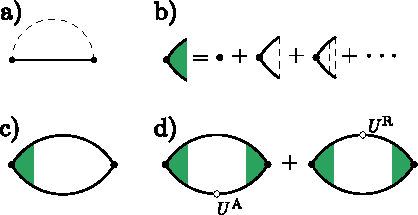
\includegraphics{articles/misha_paper/app5.pdf}
\caption{Diagrammatic illustration. a) Born-approximation. b) Ladder-approximation. c) Disorder-averaged polarization bubble. d) Perturbative expansion of the disorder-averaged polarization bubble. }
\label{chap03:fig:diagrams}
\end{figure}

In order to evaluate linear response tensors in the leading order with respect to the metal parameter $\ep\tau \gg 1$ one also needs to sum up the ladder diagrams as shown in Fig.~\ref{chap03:fig:diagrams}b-c.

To do that one defines the vertex corrected operator
\be
\label{chap03:chap3:eq:ladder}
\hat{F}^\text{vc}= \hat{F}+\hat{F}^{(1)} +\hat{F}^{(2)}+\hat{F}^{(3)}+\cdots,
\e
where we denote by $\hat{F}^{(i)}$ the operator $\hat{F}$ that is dressed by the number of $i$ disorder lines,
\be
\label{chap03:chap3:eq:onedisorderline}
\hat{F}^{(i)} = 2\pi\alpha_d\int\frac{\mathrm{d}^2\bb{p}}{(2\pi)^2} G_{\bb{p}}^\text{R}\hat{F}^{(i-1)}G_{\bb{p}}^\text{A}. 
\e
It appears that the summation in Eq.~(\ref{chap03:chap3:eq:ladder}) can be reduced to geometric series in a finite operator space. 
Indeed, let us define the operator space that is spanned by 16 operators in each of the valleys
\be
B_i=\frac{1}{2}\Lambda_\zeta\Sigma_\alpha \sigma_\beta,\quad i=\{\zeta,\alpha,\beta\},
\e
where $i$ is a cumulative index with $\zeta =0,z$ a valley parity index and $\alpha, \beta$ taking on the four values $\{0,x,y,z\}$ each. 

For $\bb{B}=(B_1, B_2,\dots, B_{32})$ we define the vertex corrected operator vector as 
\be
\label{chap03:sum}
\bb{B}^{\text{vc}}=\bb{B}+\mathcal{F}\bb{B}+\mathcal{F}^2\bb{B}+\mathcal{F}^3\bb{B}+\dots=
\frac{1}{1-\mathcal{F}}\bb{B},
\e
where $\mathcal{F}$ stands for a matrix of vertex corrections. Using the normalization condition $\tr B_i B_j =2\delta_{ij}$ 
we find
\be
\label{chap03:chap3:eq:matrixF}
\mathcal{F}_{ij} = \pi\alpha_d \int \frac{\mathrm{d}^2\bb{p}}{(2\pi)^2} 
\tr \lt[G^\text{A}_{\bb{p}} B_i G^\text{R}_{\bb{p}} B_j\rt],
\e
where $\tr$ stands for the usual matrix trace in the valley, spin and sublattice spaces.   

It easy to imagine that the matrix inversion in Eq.~(\ref{chap03:sum}) might be a daunting analytical task. We note, however, that the matrix $\mathcal{F}$ is evidently diagonal in the valley space, and it can also become block-diagonal in sublattice and spin spaces by choosing a more convenient basis. 

A particularly useful choice of basis corresponds to in-plane rotation of both spin and sublattice Pauli matrices to the frame associated with the in-plane projection $\bb{n}_\parallel$ of the N\'eel vector. For spin Pauli matrices this transformation is given by
\be
\label{chap03:trans}
\sigma_x \rightarrow \Lambda_z\frac{n_x \sigma_x + n_y \sigma_y }{\sqrt{n_x^2+n_y^2}}, \quad \sigma_y \rightarrow \Lambda_z\frac{n_y \sigma_x - n_x \sigma_y }{\sqrt{n_x^2+n_y^2}},
\e
where we took advantage of the fact that the direction of $\bb{n}$ is opposite in the two valleys. The same transformation (\ref{chap03:trans}) has to be applied to $\Sigma_{x}$ and $\Sigma_{y}$. 

The matrix $\mathcal{F}$ is instrumental for the analysis of all linear response tensors in Eq.~(\ref{chap03:tensors}). Indeed, using the definition of Eq.~(\ref{chap03:chap3:eq:matrixF}) in Eq.~(\ref{chap03:chap3:eq:kubo}) and summing up the diffusion ladders we find
\be
\label{chap03:final}
\delta s^\pm_\alpha = \frac{J^2S v^2\mathcal{A}}{2 \pi \alpha_d}
\s_\beta \s_{ij} \tr[\hat{s}^\pm_\alpha B_i] \mathcal{R}_{ij} \tr[\hat{F}_\beta B_j] \,\frac{\pa X_\beta}{\pa t},
\e
where $\mathcal{R}=\mathcal{F}(1-\mathcal{F})^{-1}$. Thus, the computation of all response tensors is reduced in the diffusive approximation to the computation of the vertex correction matrix $\mathcal{F}$ and subsequent matrix inversion.  

\section{Vertex correction}\label{chap03:sec:appc}

Still, finding an inverse matrix $(1-\mathcal{F})^{-1}$ is not that straightforward due to a pair of eigenvalues (one per valley) that equal exactly $1$. The presence of such eigenvalues roots in the particle conservation and is, therefore, not an artificial problem. The unit eigenvalues do evidently prevent the matrix inversion in Eq.~(\ref{chap03:sum}). Nevertheless, it can be shown that the corresponding eigenvectors do not enter the final equations of motion for localized spins. In the next section, we briefly illustrate how one can formally avoid the particle conservation divergence in the computation of vertex corrections.

Let us define by $\bb{a}_\zeta$ the eigenvectors of $\mathcal{F}$ that correspond to two unit eigenvalues, $\mathcal{F}\bb{a}_\zeta=\bb{a}_\zeta$, with $\zeta=0, z$. For the  normalized vector $\bb{a}_\zeta$ we define special operators
\be
\label{chap03:Bdiv}
\bar{B}_\zeta=\bb{a}_\zeta \cdot \bb{B} 
= \frac{\varepsilon-\Delta \Lambda_\zeta \Sigma_z\,\bm{n}\cdot\bm{\sigma}}{2\sqrt{\varepsilon^2+\Delta^2}},
\e
which are conserved with respect to impurity dressing $\bar{B}_\zeta=\bar{B}_\zeta^{(i)}$ for any order $i$. This means that the vertex corrected operator $\bar{B}_\zeta^\textrm{vc}$ is formally diverging in the $dc$ limit. In what follows, we formally write $\bar{B}_\zeta^{\text{vc}} = R_\infty \bar{B}_\zeta$, where the limit $R_\infty \to \infty$ is taken at the end of the calculation.

The response tensors defined by Eqs.~(\ref{chap03:response}) consist of different correlators of the operators $\Sigma_\alpha$, $s^+_\alpha=\sigma_a$, and $s^-_\alpha = \Lambda_z\Sigma_z\sigma_\alpha$. It is evident that most of these operators are already orthogonal to $\bar{B}_\zeta$,
\be
\tr \lt[\Sigma_\alpha \bar{B}_\zeta\rt] = \tr \lt[s^+_\alpha \bar{B}_\zeta\rt]= \tr \lt[s^-_\alpha \bar{B}_0\rt] =0,
\e
while the only dangerous sector is related to the projection
\be
\label{chap03:finite}
\tr \lt[s^-_\alpha \bar{B}_z\rt] = - \frac{4\Delta\, n_\alpha}{\sqrt{\varepsilon^2+\Delta^2}},
\e
which is evidently finite. The result of Eq.~(\ref{chap03:finite}) leads to formally diverging contribution $\delta \bb{s}^-_\textrm{div}$ that is generally present in all components of $\delta \bb{s}^-$, 
\be
\delta s^{-}_{\textrm{div},\alpha}\propto  R_\infty
\s_\beta \tr[\hat{\bb{s}}_\alpha^- \bar{B}_z] \tr[\hat{F}_\beta \bar{B}_z] \,\frac{\pa n_\beta}{\pa t}.
\e
One can immediately see, however, that such a diverging contribution corresponds to a particular vector form,
\be
\label{chap03:divergence}
\delta s^{-}_{\textrm{div},\alpha} \propto R_\infty n_\alpha\, \bb{n}\cdot\frac{\pa \bb{n}}{\pa t} =0,
\e
that manifestly vanishes due to the constraint $|\bb{n}|=1$ which is exact in the limit $\bb{m}=0$. Thus, the divergency in $B_\textrm{div}^\textrm{vc}$ (which originates in the diffusion pole of the density-density response) is, in fact, harmless for the response 
tensors we are discussing. 

It is interesting to note that the irrelevance of the divergency in $B_\textrm{div}^\textrm{vc}$ operator extends to higher orders in $\bb{m}$, even though it becomes much harder to see. We touch on this problem in Appendix~\ref{chap03:sec:appd}. 

\section{Finite magnetization}\label{chap03:sec:appd}
The deviation from a collinear antiferromagnetic order can be accounted by considering a finite net magnetization term in the Hamiltonain perturbatively,
\be
H =H^\textrm{eff}+ U, \qquad U = -\Delta\,\bb{m}\cdot\bb{\sigma}.
\e
In the paper, we build the first order perturbation theory with respect to $U$. 

First of all, it can be shown that the self-energy acquires the linear in $\bb{m}$ contribution as
\be\label{chap03:chap3:eq:SEcorr}
\im \Sigma^\text{R(A)} = \mp\frac{\pi\alpha_d}{2}\,(\ep-\Delta\,\Lambda_z\Sigma_z\,\bb{n}\cdot\bb{\sigma}+\Delta\,\bb{m}\cdot\bb{\sigma}).
\e
Second, the Dyson expansion of the disorder-averaged Green's functions $G^\text{R(A)}$ with respect to $\bb{m}$ reads
\be
G^\text{R(A)}\rightarrow G^\text{R(A)}+G^\text{R(A)}U^\text{R(A)}G^\text{R(A)},
\e
where $U^\text{R(A)}=U(1 \pm i \pi\alpha_d/2)$ and we disregarded terms starting from quadratic order in $\bb{m}$. Note, that 
we have kept the notations $G^\text{R(A)}$ for the disorder averaged Green's functions of the unperturbed system. 

The computation of linear response tensors amounts to considering an additional contribution to the response tensor represented by a complex class of diagrams depicted schematically in  Fig.~\ref{chap03:fig:diagrams}d. Before ladder summation is applied the diagrams of Fig.~\ref{chap03:fig:diagrams}d correspond to a contribution to the correlator of two operators $B_i$ and $B_j$ of the type 
\begin{align}
\mathcal{U}_{ij} =\,& 2\pi\alpha_d \int \frac{d^2\bb{p}}{(2\pi)^2} \tr\lt[G^\text{A} U^\text{A} G^\text{A} B_i G^R B_j\n\rt.\\
&\lt.+G^\text{A} B_i G^R U^R G^R B_j\rt],   
\end{align}
which has yet be dressed. The dressing amounts to replacing both $B_i$ and $B_j$ operators with the corresponding vertex corrected operators $B^\textrm{vc}_i$ and $B^\textrm{vc}_j$, respectively. 

The final result for the response of spin density is still given by Eq.~(\ref{chap03:final}), where the matrix $\mathcal{R}=\mathcal{F}(1-\mathcal{F})^{-1}$ is, however, replaced with 
\be
\label{chap03:chap3:eq:mresp}
\mathcal{R}=\frac{\mathcal{F}}{1-\mathcal{F}} + \frac{1}{1-\mathcal{F}}\mathcal{U}\frac{1}{1-\mathcal{F}},
\e
which corresponds to diagrams Fig.~\ref{chap03:fig:diagrams}c-d.
It is again convenient to consider a particular basis for the matrix $\mathcal{F}$ as defined in Eq.~(\ref{chap03:trans}) to simplify analytical computation.  

The problem of divergence in the operators $\bar{B}_\zeta$ does now become less trivial. Careful analysis shows that the linear terms in $\bb{m}$ included in Eq.~(\ref{chap03:chap3:eq:mresp}) lead to additional diverging contributions to $\delta\bb{s}^{-}$ of the form
\be
\label{chap03:extra}
\delta\bb{s}^{-, (1)}_{\text{div},\alpha} \propto  - R_\infty n_\alpha\, \bb{m}\cdot\frac{\pa \bb{m}}{\pa t},
\e
that is analogous to the one in Eq.~(\ref{chap03:divergence}) for a finite $m$. (We remind that the constraint $n^2+m^2=1$ provides a relation between these terms). The contribution in Eq.~(\ref{chap03:extra}) is, however, of too high order in $\bb{m}$ in Eq.~(\ref{chap03:ndot}) and cancels out completely in Eq.~(\ref{chap03:mdot}).

The terms linear in $\bb{m}$ are also responsible for diverging contributions in $\delta s_\alpha^{+}$ of the type 
\be
\delta s^{+}_{\text{div},\alpha} \propto R_\infty m_\alpha\, \bb{n}\cdot\frac{\pa \bb{n}}{\pa t}= - R_\infty m_\alpha\, \bb{m}\cdot\frac{\pa \bb{m}}{\pa t},
\e
that appear to be of higher than a linear order in $\bb{m}$, thus, exceeding our working precision.

Overall, one can show that the operators $\bar{B}_\zeta$ can be formally excluded by projecting the operator space of $B_i$ operators on the corresponding subspace. The latter is facilitated by the transformation $\mathcal{F}\to P\mathcal{F}P$, where 
\be
\label{chap03:PPP}
P= 1- \s_{\zeta=0,z}\bb{a}_\zeta \bb{a}\h_\zeta, 
\e
is the projection operator. Here, $\bb{a}$ stands for the column vector and $\bb{a}\h$ for the corresponding conjugated string vector. Eq.~(\ref{chap03:PPP}) facilitates the regularized computation of the vertex corrections and lead to the results presented in the paper.
\chapter{Research Data Management}
This thesis research has been carried out under the institute research data management policy of the Institute of Molecules and Materials of Radboud University, the Netherlands \cite{data_management_policy}.

The following datasets have been produced during this Research:

\begin{itemize}
    \item \textbf{Chapter 4:} R.J. Sokolewicz. Raw spin-density data. \emph{CNCZ, Radboud University} (2020). The dataset can be requested from the Data Officer of the Theory of Condensed Matter department, IMM, Radboud University.
\end{itemize}



%********************************************************************
% Other Stuff in the Back
%*******************************************************


\sloppy % Allow more space between words, to avoid bad boxes and hyphenating names
\cleardoublepage%********************************************************************
% Bibliography
%*******************************************************
% work-around to have small caps also here in the headline
% https://tex.stackexchange.com/questions/188126/wrong-header-in-bibliography-classicthesis
% Thanks to Enrico Gregorio
% \defbibheading{bibintoc}[\bibname]{%
%   \phantomsection
%   \manualmark
%   \markboth{\spacedlowsmallcaps{#1}}{\spacedlowsmallcaps{#1}}%
%   \addtocontents{toc}{\protect\vspace{\beforebibskip}}%
%   \addcontentsline{toc}{chapter}{\tocEntry{#1}}%
%   \chapter*{#1}%
% }
% \printbibliography[heading=bibintoc]
%\printbibliography


% \bibliographystyle{apsrev4-1}
% \bibliography{mybibliography}
% Old version, will be removed later
% work-around to have small caps also here in the headline
% \manualmark
% \markboth{\spacedlowsmallcaps{\bibname}}{\spacedlowsmallcaps{\bibname}} % work-around to have small caps also
% \phantomsection
% \refstepcounter{dummy}
% \addtocontents{toc}{\protect\vspace{\beforebibskip}} % to have the bib a bit from the rest in the toc
% \addcontentsline{toc}{chapter}{\tocEntry{\bibname}}
% \label{app:bibliography}
% \printbibliography


\fussy % Restore normal line breaking habits

\cleardoublepage%*******************************************************
% Summary
%*******************************************************
\pdfbookmark[1]{Summary}{Summary}
\phantomsection
\manualmark
\markboth{\spacedlowsmallcaps{Summary}}{\spacedlowsmallcaps{Summary}}%
\addtocontents{toc}{}%
\addcontentsline{toc}{chapter}{\tocEntry{Summary}}%
\chapter*{Summary}%
% \bigskip

\cleardoublepage%*******************************************************
% Samenvatting
%*******************************************************
\pdfbookmark[1]{Populaire Samenvatting}{Populaire samenvatting}
\phantomsection
\manualmark
\markboth{\spacedlowsmallcaps{Populaire Samenvatting}}{\spacedlowsmallcaps{Populaire Samenvatting}}%
\addtocontents{toc}{}%
\addcontentsline{toc}{chapter}{\tocEntry{Populaire Samenvatting}}%
\chapter*{Populaire Samenvatting}%
% \bigskip
In dit proefschrift wordt de interactie tussen geleidende elektronen en de magnetische momenten van atomen in een kristal bestudeerd. Deze elektronen hebben eigenschappen vergelijkbaar met die van een koelkastmagneetje, namelijk ze hebben ook een magnetisch moment, die we spin noemen. In de hedendaagse elektronica wordt voornamelijk gebruik gemaakt van de lading van de geleidende elektronen, en niet de spin. Een nieuwe generatie van elektronica die gebruikt maakt van de spin van deze geleidende elektronen wordt vaak \emph{spintronics} genoemd, en zou weleens vele voordelen kunnen bieden boven bestaande technologie. Om een paar voorbeelden te noemen, je laptop en telefoon zou met behulp van spintronica minder energie verbruiken, sneller zijn en meer foto's en video's op kunnen slaan. In de afgelopen twee decennia hebben we veel technologische vooruitgangen gezien op het gebied van spintronica, zoals het maken van elektrische stromen waar alle spins in dezelfde richting staan of het creëren van de eerste ferromagneet van 1 atoomlaag dik. 

Hoewel veel experimenten laten zien dat we magnetisme van kleine kristallen op efficiënte wijze kunnen manipuleren met behulp van elektrische stromen, en er veel fenomenologische modellen bestaan, bestaan er maar weinig microscopische modellen die uitleggen wat er nu precies gebeurt. In dit proefschrift beschouwen we een microscopisch model, waarbij de geleidende elektronen hun spin uit kunnen wisselen met de magnetische momenten in het kristal door middel van botsingen met oneffenheden in het kristal. Dit model wordt in Hoofdstuk 1 geïntroduceerd als het “s—d-model” en in Hoofdstuk 2 laten we het wiskundig kader zien waarmee we de dynamica en dissipatie van magnetische momenten in kristallen uit kunnen rekenen onder invloed van elektrische stromen. 

Ons model wordt toegepast op twee verschillende kristallen. Allereerst bestuderen we in Hoofdstuk 3 topologische halfgeleiders, die gekenmerkt worden door een sterke koppeling tussen de spin van de geleidende elektronen en hun impuls. Door een zogenaamde “top gate” te gebruiken met een zaagtand structuur, is het mogelijk om de spin van geleidende elektronen dan wel uit het kristalvlak of in het kristalvlak te laten wijzen. Naast dat dit een nieuwe manier zou zijn om de spin van geleidende elektronen te manipuleren, zou dit effect ook gebruikt kunnen worden voor het maken van een nieuw soort geheugen element. 

In de overige Hoofdstukken bestuderen we kristallen die gekenmerkt worden door een honinggraatstructuur, vergelijkbaar met grafeen, waarbij ieder atoom een magnetisch moment heeft die anti-parallel staat ten opzichte van hun buren (zie bijvoorbeeld Figuur \ref{fig:magnetic_phases} op pagina \pageref{fig:magnetic_phases}). In Hoofdstuk 4 gebruiken we een numerieke methode om de krachtmomenten uit te rekenen die geleidende elektronen uit kunnen oefenen op de magnetische momenten in het kristal. We laten zien dat deze krachtmomenten efficiënter worden als de koppeling tussen de spin van geleidende elektronen en het magnetisch moment van de atomen in het kristal asymmetrisch wordt. Dat wil zeggen, als de koppeling voor alle magnetische momenten die bijvoorbeeld omhoog wijzen anders is dan die omlaag wijzen. 

In Hoofdstuk 5 bestuderen we hetzelfde kristal, maar dit keer analytisch. Naast het uitrekenen van krachtmomenten, rekenen we ook uit hoe snel de magnetische momenten van het kristal kunnen dissiperen onder invloed van geleidende elektronen. We laten zien dat de verschillende componenten van het magnetisch moment niet alleen met andere mate dissiperen, maar ook dat de component die uit het kristalvlak wijst, behouden blijft. Met andere woorden, als we een magnetisch moment maken die uit het kristalvlak wijst kunnen we deze niet ongedaan maken met behulp van geleidende elektronen. 

In het laatste Hoofdstuk bestuderen we de rol van spin-baan koppeling op de dissipatie van magnetische momenten. We vinden hier drie regimes met een andere functionele afhankelijkheid van spin-baan koppeling op de dissipatie. Door de spin-baan koppeling te vari\"eren, kan deze afhankelijkheid experimenteel waargenomen worden met behulp van ferromagnetische resonantie, als een overgang van \emph{over}demping naar \emph{onder}demping.  


\sloppy % Allow more space between words, to avoid bad boxes and hyphenating names
\cleardoublepage\include{FrontBackmatter/publicationList}
\fussy % Restore normal line breaking habits

\cleardoublepage%*******************************************************
% Acknowledgments
%*******************************************************
\pdfbookmark[1]{Acknowledgments}{acknowledgments}
\phantomsection
\manualmark
\markboth{\spacedlowsmallcaps{Acknowledgments}}{\spacedlowsmallcaps{Acknowledgments}}%
\addtocontents{toc}{}%
\addcontentsline{toc}{chapter}{\tocEntry{Acknowledgments}}%
\chapter*{Acknowledgments}%
% \bigskip

%to include: \emph{Davis}\\ 
% This thesis would not be possible without the help and support from colleagues, friends and family. 

I have many fond memories working at the theory of condensed matter department, a place that often felt like a second home to me. Playing music on Fridays, the Seinfeld video of the day. Secretly keeping track of who entered our office and performing data analysis on it with \emph{Guus} (\emph{Lennert} won by most visits). What started as the daily coffee break with \emph{Matteo} and \emph{Alessandro}, was taken over by \emph{Achille} and \emph{Andrei}. Walking to work with \emph{Josien}. The daily zig-zag walks with \emph{Sanne}. Sharing weekend stories with \emph{Belinda}. Frequent discussions with \emph{Matthieu} about Magic: The Gathering, politics, economy and any other topic. Complaining with \emph{Taha} that our code never seems to work.
%Akwardly waving at \emph{Marion} every day. Discussing inappropriate things with \emph{Marion}. Acting crazy together with \emph{Marion} ("beeeuh").
The vodka parties at \emph{Jaap}'s place. \emph{Marion} drunkenly shouting Russian curse words at \emph{Brenner} in front of his daughter and wife. The times we played counter strike on Friday afternoon. The time \emph{Andre Bagrov} complained that the menu at caf\'e de Plak had only two meat options. 
%The time \emph{Lennert} \emph{Guus} and \emph{I} did a Monkey Island speed run and I lost miserably because I couldn't remember how to get the Jawbreaker from Cuthroat Bill.
Writing and sharing RefterPy so you can check the Refter menu from the terminal. The time \emph{Tom} accidentally used up all the computation time at Cartesius without saving any of his data. \emph{Bektur} exercising in the office to keep his focus up. Dancing with \emph{Askar}. Regretting hiking Glacier 3000 in Diablerets, Switzerland together with \emph{Misha Baglai} wearing only flip-flops. The time \emph{Zhenya} invited me to spend winter holidays in Moscow at -27 degrees. The time when \emph{Roel} and \emph{Ragnar} barged in my office singing happy birthday. After-work burgers with \emph{Ruben} and \emph{Matthieu} at the HAN student canteen. \emph{Majka} giving me surprise hugs. Walking through park Brakkenstein with \emph{David} discussing life and complaining about academia. Random coffee breaks with \emph{Thom}, lunch and dinners with \emph{Marion}. Casual visits by \emph{Bram}. %Discussing with \emph{Guus} how we could show each other something on our screens without standing up.
Discussing data privacy and many other topics with \emph{Arthur}. \emph{Annalisa}'s tiramisu. The yearly Sinterklaas celebration at TCM, in particular the time when one of the \emph{Sasha}s ate one of the presents, leaving $N-1$ gifts for $N$ people. The time another \emph{Sasha} asked if it is illegal to call the police after he was told to stop reporting the woman with a beard he saw on the street. \emph{Misha Katsnelson}'s stories about Soviet times during the coffee breaks and lunches. The countless stories of \emph{Misha Titov} involving near-death experiences, Russian aluminum mafia and children-gangs of Krasnoyarsk. The awkward silences during some of the weekly department cake breaks. The time \emph{Bob} saved \emph{Sanne} and \emph{I} with his banana we could use to bake cookies in the department's kitchen. All the brownies we ate. Not being able to graduate my Master's in time, because I forgot to hand in a report for a course of \emph{Shengjun}.
% All the times \emph{I} baked brownies and apple pies.
The time \emph{Ivan} retrieved his stolen hard drive from the Camorra. All the times when \emph{Koen} effortlessly shows his communication skills in 4.5 different languages. Playing jianzi with \emph{Edo}, \emph{Peilang}, \emph{Jin}, \emph{Guodong} and \emph{Amanda}. Discussing TikZ with \emph{Erik}. 
%Random games of chess with \emph{Peilang}, \emph{Misha Titov}, and \emph{Askar}.
Dressing up as pikachu to make a PhD video for \emph{Remko}. \emph{Hylke} being the first to join for Friday afternoon drinks. The time all participants of a summer school in Moscow ended up with a week long diarrhea after food poisoning. Sharing craft-beer enthusiasm with \emph{Dima}. Ice skating with \emph{Mariana}, tennis with \emph{Lisa}. The time \emph{Manuel} took over my apartment. The time I randomly met \emph{Michel}, \emph{Clement}'s best friend, in a bar in Leiden.  
% The time we built a five meter snow-penis in front of \emph{Zhenya}'s office.
%The time \emph{Lennert}, \emph{Erik}, \emph{Edo} and \emph{I} took an afternoon off to play a 3 hour game of Shogun.

Outside of work, many good times could be found as well. The time \emph{Andre}, \emph{Matteo} and \emph{I} surprised \emph{Samy} in Toulouse. Sunday evening board game nights. The time \emph{Dave}, \emph{Cas}, \emph{Clarisse} and \emph{Jos} pushed me to join a cooking show when I was hungover. The times that \emph{M\'elanie} shared stories from the hospital's urology department she worked at. Partying with \emph{Pam}. Celebrating \emph{Bj\"orn}'s birthday party at his summer house in \"Oland, Sweden. 
Creating ugly Christmas card photos with \emph{Bram} and \emph{Thom}. The time I hiked up the Sanctuary of the Madonna di San Luca with \emph{Lennart}. 
%All the times playing Magic: The Gathering in Arnhem with \emph{Ruben}, \emph{Matthieu} and in Nijmegen with \emph{Joost} and \emph{Derrick}.
Brewing beer with the \emph{brouwcie} in front of the university sports center, with \emph{Nick} and \emph{Edo} in Utrecht, or on \emph{Ruben}'s balcony with \emph{Ruben} and \emph{Matthieu}. The time we went indoor-skiing with \emph{Wen}, \emph{Edo} and \emph{Marion}. Playing badminton with \emph{Kate} in Kleve. The times \emph{Fabries} shows how easy it is to beat me at Hearthstone. Partying with \emph{Laura} and \emph{Marcella}. Going to the gym with \emph{Robert} and \emph{Jop}. Playing a horror survival game with the lights out with \emph{Kiki}. The time we went to the casino with \emph{Dave}, \emph{Yolanda} and \emph{Jesus} during the vierdaagsefeesten.  Visiting \emph{Judith} in Essen. Going to the down the rabbit hole-festival every other year and many other activities with \emph{Jop}, \emph{Thom}, \emph{Bram}, \emph{Edo}, \emph{Bob}, \emph{Majka}, \emph{Sanne}, \emph{Josien}, \emph{Arthur}, \emph{Judith}, \emph{Kiane}, \emph{Maren}, \emph{Sam}, \emph{Sander}, \emph{Vera}, \emph{Yvonne}, \emph{Belle} \& \emph{Guido}. \\[0.5em]

Of course, a special thanks to my \emph{parents}. Faworki and lemon cake on my birthdays, dinners every weekend. The countless times I receive good advice. The big influence my brother, \emph{Maciek}, had on me while growing up. The times you taught me how to build a calculator in php and how to use regular expressions when I was just 13 years old.  \\[0.5em]

And of course, spending the last two months of my PhD in lockdown with my sweet and lovely girlfriend, \emph{Lan}$\heartsuit$.

\begin{flushright} - \emph{Robert Sokolewicz, October 2020}\end{flushright}

\cleardoublepage%*******************************************************
% Publications
%*******************************************************
\pdfbookmark[1]{Curriculum Vitae}{Curriculum Vitae}
\phantomsection
\manualmark
\markboth{\spacedlowsmallcaps{Curriculum Vitae}}{\spacedlowsmallcaps{Curriculum Vitae}}%
\addtocontents{toc}{}%
\addcontentsline{toc}{chapter}{\tocEntry{Curriculum Vitae}}%
\chapter*{Curriculum Vitae}%

Robert Sokolewicz was born on 7th of February 1990 in Delft, the Netherlands. He grew up in Nijmegen and received his pre-university education at the Nijmeegse Scholengemeenschap Groenewoud from 2002 until 2009. In 2009, Robert started his studies in physics and astronomy at the Radboud University. He wrote his bachelor thesis at the department of Theory of Condensed Matter under the supervision of dr. Timur Tudorovskiy and later his master thesis at the same department under supervision of dr. Mikhail Titov. After obtaining his Master of Science degree in 2016 (cum laude), he started his PhD research under the supervision of prof. dr. Mikhail Katsnelson and dr. Mikhail Titov. Robert currently works as a postdoc at the Theory of Condensed Matter department of
the Radboud University.

\cleardoublepage

% \cleardoublepage%********************************************************************
% Bibliography
%*******************************************************
% work-around to have small caps also here in the headline
% https://tex.stackexchange.com/questions/188126/wrong-header-in-bibliography-classicthesis
% Thanks to Enrico Gregorio
% \defbibheading{bibintoc}[\bibname]{%
%   \phantomsection
%   \manualmark
%   \markboth{\spacedlowsmallcaps{#1}}{\spacedlowsmallcaps{#1}}%
%   \addtocontents{toc}{\protect\vspace{\beforebibskip}}%
%   \addcontentsline{toc}{chapter}{\tocEntry{#1}}%
%   \chapter*{#1}%
% }
% \printbibliography[heading=bibintoc]
%\printbibliography


% \bibliographystyle{apsrev4-1}
% \bibliography{mybibliography}
% Old version, will be removed later
% work-around to have small caps also here in the headline
% \manualmark
% \markboth{\spacedlowsmallcaps{\bibname}}{\spacedlowsmallcaps{\bibname}} % work-around to have small caps also
% \phantomsection
% \refstepcounter{dummy}
% \addtocontents{toc}{\protect\vspace{\beforebibskip}} % to have the bib a bit from the rest in the toc
% \addcontentsline{toc}{chapter}{\tocEntry{\bibname}}
% \label{app:bibliography}
% \printbibliography



\cleardoublepage\pagestyle{empty}

\hfill

\vfill


\pdfbookmark[0]{Colophon}{colophon}
\section*{Colophon}

\bigskip

\noindent\finalVersionString

%Hermann Zapf's \emph{Palatino} and \emph{Euler} type faces (Type~1 PostScript fonts \emph{URW
%Palladio L} and \emph{FPL}) are used. The ``typewriter'' text is typeset in \emph{Bera Mono},
%originally developed by Bitstream, Inc. as ``Bitstream Vera''. (Type~1 PostScript fonts were made
%available by Malte Rosenau and
%Ulrich Dirr.)

%\paragraph{note:} The custom size of the textblock was calculated
%using the directions given by Mr. Bringhurst (pages 26--29 and
%175/176). 10~pt Palatino needs  133.21~pt for the string
%``abcdefghijklmnopqrstuvwxyz''. This yields a good line length between
%24--26~pc (288--312~pt). Using a ``\emph{double square textblock}''
%with a 1:2 ratio this results in a textblock of 312:624~pt (which
%includes the headline in this design). A good alternative would be the
%``\emph{golden section textblock}'' with a ratio of 1:1.62, here
%312:505.44~pt. For comparison, \texttt{DIV9} of the \texttt{typearea}
%package results in a line length of 389~pt (32.4~pc), which is by far
%too long. However, this information will only be of interest for
%hardcore pseudo-typographers like me.%
%
%To make your own calculations, use the following commands and look up
%the corresponding lengths in the book:
%\begin{verbatim}
%    \settowidth{\abcd}{abcdefghijklmnopqrstuvwxyz}
%    \the\abcd\ % prints the value of the length
%\end{verbatim}
%Please see the file \texttt{classicthesis.sty} for some precalculated
%values for Palatino and Minion.
%
%    \settowidth{\abcd}{abcdefghijklmnopqrstuvwxyz}
%    \the\abcd\ % prints the value of the length

% ********************************************************************
% Game Over: Restore, Restart, or Quit?
%*******************************************************
\end{document}
% ********************************************************************

